\documentclass[titlepage,numbers=noenddot,headinclude,
                footinclude=true,abstractoff,
                BCOR=5mm,paper=letter,fontsize=11pt,
                ngerman,american,dottedtoc]{scrreprt}

% ****************************************************************************************************
% classicthesis-config.tex
% formerly known as loadpackages.sty, classicthesis-ldpkg.sty, and classicthesis-preamble.sty
% Use it at the beginning of your ClassicThesis.tex, or as a LaTeX Preamble
% in your ClassicThesis.{tex,lyx} with \input{classicthesis-config}
% ****************************************************************************************************
% If you like the classicthesis, then I would appreciate a postcard.
% My address can be found in the file ClassicThesis.pdf. A collection
% of the postcards I received so far is available online at
% http://postcards.miede.de
% ****************************************************************************************************


% ****************************************************************************************************
% 0. Set the encoding of your files. UTF-8 is the only sensible encoding nowadays. If you can't read
% äöüßáéçèê∂åëæƒÏ€ then change the encoding setting in your editor, not the line below. If your editor
% does not support utf8 use another editor!
% ****************************************************************************************************
\PassOptionsToPackage{utf8}{inputenc}
	\usepackage{inputenc}
%\usepackage{tikz}
% ****************************************************************************************************
% 1. Configure classicthesis for your needs here, e.g., remove "drafting" below
% in order to deactivate the time-stamp on the pages
% ****************************************************************************************************
\PassOptionsToPackage{eulerchapternumbers,listings,%
					 pdfspacing,floatperchapter,%linedheaders,%
					 subfig,beramono,eulermath,parts}{linux_introduction}
% ********************************************************************
% Available options for classicthesis.sty
% (see ClassicThesis.pdf for more information):
% drafting
% parts nochapters linedheaders
% eulerchapternumbers beramono eulermath pdfspacing minionprospacing
% tocaligned dottedtoc manychapters
% listings floatperchapter subfig
% ********************************************************************


% ****************************************************************************************************
% 2. Personal data and user ad-hoc commands
% ****************************************************************************************************
\newcommand{\myTitle}{Introduction to Linux\xspace}
\newcommand{\mySubtitle}{An Homage to The Elements of Typographic Style\xspace}
\newcommand{\myDegree}{Doktor-Ingenieur (Dr.-Ing.)\xspace}
\newcommand{\myName}{Marcel Jar\xspace}
\newcommand{\myProf}{Put name here\xspace}
\newcommand{\myOtherProf}{Put name here\xspace}
\newcommand{\mySupervisor}{Put name here\xspace}
\newcommand{\myFaculty}{Put data here\xspace}
\newcommand{\myDepartment}{Put data here\xspace}
\newcommand{\myUni}{Put data here\xspace}
\newcommand{\myLocation}{Saarbrücken\xspace}
\newcommand{\myTime}{September 2015\xspace}
\newcommand{\myVersion}{version 4.2\xspace}

% ********************************************************************
% Setup, finetuning, and useful commands
% ********************************************************************
\newcounter{dummy} % necessary for correct hyperlinks (to index, bib, etc.)
\newlength{\abcd} % for ab..z string length calculation
\providecommand{\mLyX}{L\kern-.1667em\lower.25em\hbox{Y}\kern-.125emX\@}
\newcommand{\ie}{i.\,e.}
\newcommand{\Ie}{I.\,e.}
\newcommand{\eg}{e.\,g.}
\newcommand{\Eg}{E.\,g.}
% ****************************************************************************************************


% ****************************************************************************************************
% 3. Loading some handy packages
% ****************************************************************************************************
% ********************************************************************
% Packages with options that might require adjustments
% ********************************************************************
\usepackage{makeidx}
%\PassOptionsToPackage{ngerman,american}{babel}   % change this to your language(s)
% Spanish languages need extra options in order to work with this template
%\PassOptionsToPackage{spanish,es-lcroman}{babel}
	\usepackage{babel}

\usepackage{csquotes}
\PassOptionsToPackage{%
    %backend=biber, %instead of bibtex
	backend=bibtex8,bibencoding=ascii,%
	language=auto,%
	style=numeric-comp,%
    %style=authoryear-comp, % Author 1999, 2010
    %bibstyle=authoryear,dashed=false, % dashed: substitute rep. author with ---
    sorting=nyt, % name, year, title
    maxbibnames=10, % default: 3, et al.
    %backref=true,%
    natbib=true % natbib compatibility mode (\citep and \citet still work)
}{biblatex}
    \usepackage{biblatex}

\PassOptionsToPackage{fleqn}{amsmath}       % math environments and more by the AMS
    \usepackage{amsmath}

% ********************************************************************
% General useful packages
% ********************************************************************
\PassOptionsToPackage{T1}{fontenc} % T2A for cyrillics
    \usepackage{fontenc}
\usepackage{textcomp} % fix warning with missing font shapes
\usepackage{scrhack} % fix warnings when using KOMA with listings package
\usepackage{xspace} % to get the spacing after macros right
\usepackage{mparhack} % get marginpar right
\usepackage{fixltx2e} % fixes some LaTeX stuff --> since 2015 in the LaTeX kernel (see below)
%\usepackage[latest]{latexrelease} % will be used once available in more distributions (ISSUE #107)
\PassOptionsToPackage{printonlyused,smaller}{acronym}
    \usepackage{acronym} % nice macros for handling all acronyms in the thesis
    %\renewcommand{\bflabel}[1]{{#1}\hfill} % fix the list of acronyms --> no longer working
    %\renewcommand*{\acsfont}[1]{\textsc{#1}}
    \renewcommand*{\aclabelfont}[1]{\acsfont{#1}}
% ****************************************************************************************************


% ****************************************************************************************************
% 4. Setup floats: tables, (sub)figures, and captions
% ****************************************************************************************************
\usepackage{tabularx} % better tables
    \setlength{\extrarowheight}{3pt} % increase table row height
\newcommand{\tableheadline}[1]{\multicolumn{1}{c}{\spacedlowsmallcaps{#1}}}
\newcommand{\myfloatalign}{\centering} % to be used with each float for alignment
\usepackage{caption}
% Thanks to cgnieder and Claus Lahiri
% http://tex.stackexchange.com/questions/69349/spacedlowsmallcaps-in-caption-label
% [REMOVED DUE TO OTHER PROBLEMS, SEE ISSUE #82]
%\DeclareCaptionLabelFormat{smallcaps}{\bothIfFirst{#1}{~}\MakeTextLowercase{\textsc{#2}}}
%\captionsetup{font=small,labelformat=smallcaps} % format=hang,
\captionsetup{font=small} % format=hang,
\usepackage{subfig}
% ****************************************************************************************************


% ****************************************************************************************************
% 5. Setup code listings
% ****************************************************************************************************
\usepackage{listings}
%\lstset{emph={trueIndex,root},emphstyle=\color{BlueViolet}}%\underbar} % for special keywords
\lstset{language=[LaTeX]Tex,%C++,
    morekeywords={PassOptionsToPackage,selectlanguage},
    keywordstyle=\color{RoyalBlue},%\bfseries,
    basicstyle=\small\ttfamily,
    %identifierstyle=\color{NavyBlue},
    commentstyle=\color{Green}\ttfamily,
    stringstyle=\rmfamily,
    %numbers=none,%left,%
    %numberstyle=\scriptsize,%\tiny
    %stepnumber=5,
    %numbersep=8pt,
    showstringspaces=false,
    %breaklines=true,
    %frameround=ftff,
    %frame=single,
    belowcaptionskip=.75\baselineskip
    %frame=L
}

\usepackage{courier}
\usepackage{color}
\definecolor{codegreen}{rgb}{0,0.6,0}
\definecolor{codegray}{rgb}{0.5,0.5,0.5}
\definecolor{codepurple}{rgb}{0.58,0,0.82}
\definecolor{backcolour}{rgb}{0.95,0.95,0.92}
\lstdefinestyle{numbers}{
   backgroundcolor=\color{backcolour},
   commentstyle=\color{codegreen},
   keywordstyle=\color{magenta},
   stringstyle=\color{codepurple},
   numberstyle=\normalsize\color{codegray},
   basicstyle=\normalsize\ttfamily,
   breakatwhitespace=false,
   breaklines=true,
   captionpos=b,
   keepspaces=true,
   numbers=left,
   numbersep=5pt,
   showspaces=false,
   showstringspaces=false,
   showtabs=false,
   tabsize=2
}

\lstdefinestyle{nonumbers}{
   backgroundcolor=\color{backcolour},
   commentstyle=\color{codegreen},
   keywordstyle=\color{magenta},
   stringstyle=\color{codepurple},
   numberstyle=\normalsize\color{codegray},
   basicstyle=\normalsize\ttfamily,
   breakatwhitespace=false,
   breaklines=true,
   captionpos=b,
   keepspaces=true,
   numbers=none,
   numbersep=5pt,
   showspaces=false,
   showstringspaces=false,
   showtabs=false,
   tabsize=2
}

\lstnewenvironment{source_code}[1][Bash]
{\lstset{style=numbers, language=#1, moredelim={[is][\bfseries]{@@}{@@}}}}
{}


\lstnewenvironment{source_code_float}[3]
{\lstset{style=numbers, language=#1, float=!ht, caption={#2},label=#3,moredelim={[is][\bfseries]{@@}{@@}}}}
{}

\lstnewenvironment{command_line}[1][Bash]
{\lstset{style=nonumbers, language=#1, moredelim={[is][\bfseries]{@@}{@@}}}}
{}

\lstnewenvironment{command_line_float}[3]
{\lstset{style=nonumbers, language=#1, float=!ht, caption={#2},label=#3,moredelim={[is][\bfseries]{@@}{@@}}}}
{}

% ****************************************************************************************************


% ****************************************************************************************************
% 6. PDFLaTeX, hyperreferences and citation backreferences
% ****************************************************************************************************
% ********************************************************************
% Using PDFLaTeX
% ********************************************************************
\PassOptionsToPackage{pdftex,hyperfootnotes=false,pdfpagelabels}{hyperref}
    \usepackage{hyperref}  % backref linktocpage pagebackref
\pdfcompresslevel=9
\pdfadjustspacing=1
\PassOptionsToPackage{pdftex}{graphicx}
    \usepackage{graphicx}


% ********************************************************************
% Hyperreferences
% ********************************************************************
\hypersetup{%
    %draft, % = no hyperlinking at all (useful in b/w printouts)
    colorlinks=true, linktocpage=true, pdfstartpage=3, pdfstartview=FitV,%
    % uncomment the following line if you want to have black links (e.g., for printing)
    %colorlinks=false, linktocpage=false, pdfstartpage=3, pdfstartview=FitV, pdfborder={0 0 0},%
    breaklinks=true, pdfpagemode=UseNone, pageanchor=true, pdfpagemode=UseOutlines,%
    plainpages=false, bookmarksnumbered, bookmarksopen=true, bookmarksopenlevel=1,%
    hypertexnames=true, pdfhighlight=/O,%nesting=true,%frenchlinks,%
    urlcolor=webbrown, linkcolor=RoyalBlue, citecolor=webgreen, %pagecolor=RoyalBlue,%
    %urlcolor=Black, linkcolor=Black, citecolor=Black, %pagecolor=Black,%
    pdftitle={\myTitle},%
    pdfauthor={\textcopyright\ \myName, \myUni, \myFaculty},%
    pdfsubject={},%
    pdfkeywords={},%
    pdfcreator={pdfLaTeX},%
    pdfproducer={LaTeX with hyperref and classicthesis}%
}

% ********************************************************************
% Setup autoreferences
% ********************************************************************
% There are some issues regarding autorefnames
% http://www.ureader.de/msg/136221647.aspx
% http://www.tex.ac.uk/cgi-bin/texfaq2html?label=latexwords
% you have to redefine the makros for the
% language you use, e.g., american, ngerman
% (as chosen when loading babel/AtBeginDocument)
% ********************************************************************
\makeatletter
\@ifpackageloaded{babel}%
    {%
       \addto\extrasamerican{%
			\renewcommand*{\figureautorefname}{Figure}%
			\renewcommand*{\tableautorefname}{Table}%
			\renewcommand*{\partautorefname}{Part}%
			\renewcommand*{\chapterautorefname}{Chapter}%
			\renewcommand*{\sectionautorefname}{Section}%
			\renewcommand*{\subsectionautorefname}{Section}%
			\renewcommand*{\subsubsectionautorefname}{Section}%
                }%
       \addto\extrasngerman{%
			\renewcommand*{\paragraphautorefname}{Absatz}%
			\renewcommand*{\subparagraphautorefname}{Unterabsatz}%
			\renewcommand*{\footnoteautorefname}{Fu\"snote}%
			\renewcommand*{\FancyVerbLineautorefname}{Zeile}%
			\renewcommand*{\theoremautorefname}{Theorem}%
			\renewcommand*{\appendixautorefname}{Anhang}%
			\renewcommand*{\equationautorefname}{Gleichung}%
			\renewcommand*{\itemautorefname}{Punkt}%
                }%
            % Fix to getting autorefs for subfigures right (thanks to Belinda Vogt for changing the definition)
            \providecommand{\subfigureautorefname}{\figureautorefname}%
    }{\relax}
\makeatother


% ****************************************************************************************************
% 7. Last calls before the bar closes
% ****************************************************************************************************
% ********************************************************************
% Development Stuff
% ********************************************************************
\listfiles
%\PassOptionsToPackage{l2tabu,orthodox,abort}{nag}
%   \usepackage{nag}
%\PassOptionsToPackage{warning, all}{onlyamsmath}
%   \usepackage{onlyamsmath}

% ********************************************************************
% Last, but not least...
% ********************************************************************
\usepackage{linux_introduction}
% ****************************************************************************************************


% ****************************************************************************************************
% 8. Further adjustments (experimental)
% ****************************************************************************************************
% ********************************************************************
% Changing the text area
% ********************************************************************
%\linespread{1.05} % a bit more for Palatino
%\areaset[current]{312pt}{761pt} % 686 (factor 2.2) + 33 head + 42 head \the\footskip
%\setlength{\marginparwidth}{7em}%
%\setlength{\marginparsep}{2em}%

% ********************************************************************
% Using different fonts
% ********************************************************************
%\usepackage[oldstylenums]{kpfonts} % oldstyle notextcomp
%\usepackage[osf]{libertine}
%\usepackage[light,condensed,math]{iwona}
%\renewcommand{\sfdefault}{iwona}
%\usepackage{lmodern} % <-- no osf support :-(
%\usepackage{cfr-lm} %
%\usepackage[urw-garamond]{mathdesign} <-- no osf support :-(
%\usepackage[default,osfigures]{opensans} % scale=0.95
%\usepackage[sfdefault]{FiraSans}
% ****************************************************************************************************


\addbibresource{Bibliography.bib}
\addbibresource[label=ownpubs]{AMiede_Publications.bib}
%\usepackage[active,tightpage]{preview}

%\hyphenation{put special hyphenation here}

\makeindex

\begin{document}
\frenchspacing
\raggedbottom
\selectlanguage{american} % american ngerman
%\renewcommand*{\bibname}{new name}
%\setbibpreamble{}
\pagenumbering{roman}
\pagestyle{plain}

%********************************************************************
% Frontmatter
%*******************************************************
%%*******************************************************
% Little Dirty Titlepage
%*******************************************************
\thispagestyle{empty}
%\pdfbookmark[1]{Titel}{title}
%*******************************************************
\begin{center}
    \spacedlowsmallcaps{\myName} \\ \medskip                        

    \begingroup
        \color{Maroon}\spacedallcaps{\myTitle}
    \endgroup
\end{center}        

%*******************************************************
% Titlepage
%*******************************************************
\begin{titlepage}
    % if you want the titlepage to be centered, uncomment and fine-tune the line below (KOMA classes environment)
    %\begin{addmargin}[-1cm]{-3cm}
    \begin{center}
        \large  

        \hfill

        \vfill

        \begingroup
            \color{Maroon}\spacedallcaps{\myTitle} \\ \bigskip
        \endgroup

        \spacedlowsmallcaps{\myName}

        \vfill

        %
\includegraphics[width=6cm]{gfx/TFZsuperellipse_bw} \\ \medskip

        %\mySubtitle \\ \medskip   
        %\myDegree \\
        %\myDepartment \\                            
        %\myFaculty \\
        %\myUni \\ \bigskip

        %\myTime\ -- \myVersion

        \vfill                      

    \end{center}  
  %\end{addmargin}       
\end{titlepage}   
%\thispagestyle{empty}

\hfill

\vfill

\noindent\myName: \textit{\myTitle,} \mySubtitle, %\myDegree, 
\textcopyright\ \myTime

%\bigskip
%
%\noindent\spacedlowsmallcaps{Supervisors}: \\
%\myProf \\
%\myOtherProf \\ 
%\mySupervisor
%
%\medskip
%
%\noindent\spacedlowsmallcaps{Location}: \\
%\myLocation
%
%\medskip
%
%\noindent\spacedlowsmallcaps{Time Frame}: \\
%\myTime

%\cleardoublepage%*******************************************************
% Dedication
%*******************************************************
\thispagestyle{empty}
%\phantomsection 
\refstepcounter{dummy}
\pdfbookmark[1]{Dedication}{Dedication}

\vspace*{3cm}

\begin{center}
    \emph{Ohana} means family. \\
    Family means nobody gets left behind, or forgotten. \\ \medskip
    --- Lilo \& Stitch    
\end{center}

\medskip

\begin{center}
    Dedicated to the loving memory of Rudolf Miede. \\ \smallskip
    1939\,--\,2005
\end{center}
%\cleardoublepage\include{FrontBackmatter/Foreword}
%\cleardoublepage%*******************************************************
% Abstract
%*******************************************************
%\renewcommand{\abstractname}{Abstract}
\pdfbookmark[1]{Abstract}{Abstract}
\begingroup
\let\clearpage\relax
\let\cleardoublepage\relax
\let\cleardoublepage\relax

\chapter*{Abstract}
Short summary of the contents in English\dots a great guide by 
Kent Beck how to write good abstracts can be found here:  
\begin{center}
\url{https://plg.uwaterloo.ca/~migod/research/beckOOPSLA.html}
\end{center}

\vfill

\begin{otherlanguage}{ngerman}
\pdfbookmark[1]{Zusammenfassung}{Zusammenfassung}
\chapter*{Zusammenfassung}
Kurze Zusammenfassung des Inhaltes in deutscher Sprache\dots 
\end{otherlanguage}

\endgroup			

\vfill
%\cleardoublepage%*******************************************************
% Publications
%*******************************************************
\pdfbookmark[1]{Publications}{publications}
\chapter*{Publications}\graffito{This is just an early --~and currently ugly~-- test!}
This might come in handy for PhD theses: some ideas and figures have appeared previously in the following publications:

%\noindent Put your publications from the thesis here. The packages \texttt{multibib} or \texttt{bibtopic} etc. can be used to handle multiple different bibliographies in your document.

\begin{refsection}[ownpubs]
    \small
    \nocite{*} % is local to to the enclosing refsection
    \printbibliography[heading=none]
\end{refsection}

\emph{Attention}: This requires a separate run of \texttt{bibtex} for your \texttt{refsection}, \eg, \texttt{ClassicThesis1-blx} for this file. You might also use \texttt{biber} as the backend for \texttt{biblatex}. See also \url{http://tex.stackexchange.com/questions/128196/problem-with-refsection}.
%\cleardoublepage%*******************************************************
% Acknowledgments
%*******************************************************
\pdfbookmark[1]{Acknowledgments}{acknowledgments}

\begin{flushright}{\slshape    
    We have seen that computer programming is an art, \\ 
    because it applies accumulated knowledge to the world, \\ 
    because it requires skill and ingenuity, and especially \\
    because it produces objects of beauty.} \\ \medskip
    --- \defcitealias{knuth:1974}{Donald E. Knuth}\citetalias{knuth:1974} \citep{knuth:1974}
\end{flushright}



\bigskip

\begingroup
\let\clearpage\relax
\let\cleardoublepage\relax
\let\cleardoublepage\relax
\chapter*{Acknowledgments}
Put your acknowledgments here.

Many thanks to everybody who already sent me a postcard!

Regarding the typography and other help, many thanks go to Marco 
Kuhlmann, Philipp Lehman, Lothar Schlesier, Jim Young, Lorenzo 
Pantieri and Enrico Gregorio\footnote{Members of GuIT (Gruppo 
Italiano Utilizzatori di \TeX\ e \LaTeX )}, J\"org Sommer, 
Joachim K\"ostler, Daniel Gottschlag, Denis Aydin, Paride 
Legovini, Steffen Prochnow, Nicolas Repp, Hinrich Harms, 
 Roland Winkler, Jörg Weber, Henri Menke, Claus Lahiri, 
 Clemens Niederberger, Stefano Bragaglia, Jörn Hees, 
 and the whole \LaTeX-community for support, ideas and 
 some great software.

\bigskip

\noindent\emph{Regarding \mLyX}: The \mLyX\ port was intially done by 
\emph{Nicholas Mariette} in March 2009 and continued by 
\emph{Ivo Pletikosi\'c} in 2011. Thank you very much for your 
work and for the contributions to the original style.


\endgroup




\pagestyle{scrheadings}
\cleardoublepage%*******************************************************
% Table of Contents
%*******************************************************
%\phantomsection
\refstepcounter{dummy}
\pdfbookmark[1]{\contentsname}{tableofcontents}
\setcounter{tocdepth}{2} % <-- 2 includes up to subsections in the ToC
\setcounter{secnumdepth}{3} % <-- 3 numbers up to subsubsections
\manualmark
\markboth{\spacedlowsmallcaps{\contentsname}}{\spacedlowsmallcaps{\contentsname}}
\tableofcontents
\automark[section]{chapter}
\renewcommand{\chaptermark}[1]{\markboth{\spacedlowsmallcaps{#1}}{\spacedlowsmallcaps{#1}}}
\renewcommand{\sectionmark}[1]{\markright{\thesection\enspace\spacedlowsmallcaps{#1}}}
%*******************************************************
% List of Figures and of the Tables
%*******************************************************
\clearpage

\begingroup
    \let\clearpage\relax
    \let\cleardoublepage\relax
    \let\cleardoublepage\relax
    %*******************************************************
    % List of Figures
    %*******************************************************
    %\phantomsection
    \refstepcounter{dummy}
    %\addcontentsline{toc}{chapter}{\listfigurename}
    \pdfbookmark[1]{\listfigurename}{lof}
    \listoffigures

    \vspace{8ex}

    %*******************************************************
    % List of Tables
    %*******************************************************
    %\phantomsection
    \refstepcounter{dummy}
    %\addcontentsline{toc}{chapter}{\listtablename}
    \pdfbookmark[1]{\listtablename}{lot}
    \listoftables

    \vspace{8ex}
%   \newpage

    %*******************************************************
    % List of Listings
    %*******************************************************
      %\phantomsection
    \refstepcounter{dummy}
    %\addcontentsline{toc}{chapter}{\lstlistlistingname}
    \pdfbookmark[1]{\lstlistlistingname}{lol}
    \lstlistoflistings

    \vspace{8ex}

    %*******************************************************
    % Acronyms
    %*******************************************************
    %\phantomsection
    \refstepcounter{dummy}
    \pdfbookmark[1]{Acronyms}{acronyms}
    \markboth{\spacedlowsmallcaps{Acronyms}}{\spacedlowsmallcaps{Acronyms}}
    \chapter*{Acronyms}
    \begin{acronym}[UMLX]
        \acro{DRY}{Don't Repeat Yourself}
        \acro{API}{Application Programming Interface}
        \acro{CLI}{Command Line Interface}
        \acro{GUI}{Graphical User Interface}
        \acro{UI}{User Interface}
        \acro{UML}{Unified Modeling Language}
        \acro{OS}{Operating System}
        \acro{FHS}{File system Hierarchy Standard}
        \acro{PC}{Personal Computer}
        \acro{GNU}{GNU is Not Unix}
        \acro{FSF}{Free Software Foundation}
        \acro{CPU}{Central Processing Unit}
        \acro{RAM}{Random Access Memory}
        \acro{HD}{Hard Disk}
        \acro{SSD}{Solid State Device}
    \end{acronym}
\endgroup


%********************************************************************
% Mainmatter
%*******************************************************
\cleardoublepage
\pagenumbering{arabic}
%\setcounter{page}{90}
% use \cleardoublepage here to avoid problems with pdfbookmark
\cleardoublepage
\ctparttext{In the following chapters, we explain what an operating system is, as well as its relationship with the computer hardware and software applications. Following, we present a brief overview of Linux's history. Finally, we discuss what Linux distributions are, and we comment on some of the defining characteristics of some of the most widely used distributions.}
\part{Introduction to Command Line Interfaces}
%************************************************
\chapter{What is an Operating System}\label{ch:os}
%************************************************

To understand Linux Operating Systems, it is necessary first to understand what an Operating System (\acs{OS}) is. In a nutshell, an operating system is a fundamental piece software that manages both hardware and software resources, while also providing users with a set of core utilities.


\section{Operating System Components}

An \acs{OS} is normally divided in many components in order to make the different parts of a computer work together. Amongst those components, it is worth to cite:
\begin{description}
\item[kernel] The kernel is the most crucial part of any \acs{OS}. It serves as an intermediate between software applications and the hardware, having complete control over everything that happens in the system. It controls which software processes are running at any given time, how much memory each process is assigned to, and also provide a gateway between these processes and hardware such as printers, network cards, keyboards, etc.
\item[user interface] In order to be useful, an \acs{OS} needs to provide users with a way to access the data stored in it, as well as run different types of applications. In the past, most \acs{OS}s had only command line interfaces. However, most modern systems nowadays provide users with increasingly easier to use graphical user interfaces.
\item[File system] The responsibility to store and retrieve data into/from memory devices, as well as ensure that it hasn't been corrupted, belongs to the \acs{OS}.
\item[Security] Any respectable \acs{OS} must provide methods for users to control access to the system itself, as well as to control access to individual files and processes.
\item[Core utilities] The \acs{OS} is also expected to provide the user with basic utilities to perform things such as: find files, edit text files, control system settings, control processes, etc.
\end{description}

Probably, the most famous \acs{OS} is Microsoft Windows, whose version 10 now comes installed by default in a large number of laptops and desktops. It is easy to see that Windows has all the components described above, as seen in Table \ref{tab:windows_os}.

\begin{table}[!htbp]
   \myfloatalign
   \begin{tabularx}{\textwidth}{Xp{85mm}} \toprule
   %\tableheadline{Shell} & \tableheadline{Description}\\ \midrule
   \textbf{Kernel} & The Windows kernel contains a large set of device drivers that allows it to interact with a very wide array of hardware components, from external keyboards to virtual reality glasses. It is able to run multiple applications at once, and allow users to control which applications get more priority. \\
   \textbf{User Interface} &  The graphical interface for Windows is classicaly composed of a Start Buttom, a Taskbar, as well as ``Windows,'' where each ``Window'' normally correspond to an specific application. \\
   \textbf{File System} & Windows is normally installed using an NTFS file system that ensures the reliability of the stored data.\\
   \textbf{Security} & Windows provides control access to the system, as you normally need to enter a password to access it. Also, some versions of Windows allow users to set specif access rights to individual files.\\
   \textbf{Core Utilities} & Windows comes with multiple core utilities such as: File Explorer to retrieve any file in its memory, Notepad to edit text files, Control Panel to modify systems settings, etc.\\

\bottomrule
   \end{tabularx}
\caption{Windows \acs{OS} Components.}
\label{tab:windows_os}
\end{table}

\section{Computer Architecture Basics}

In order to better appreciate the role the kernel, it is important to understand the architecture of modern computers. In Figure~\ref{fig:cha_kernel}, you can see how the kernel fits within a basic computer architecture. In it, it is clear that the kernel acts as a bridge between applications (at the top), and hardware components (at the bottom). Note that the kernel also provides a bridge between different applications, as well as different hardware components.

\begin{figure}[!htbp]
  \centering
        \documentclass{standalone}

\usepackage{tikz}
\usetikzlibrary{trees}
\usepgflibrary{arrows}
\usetikzlibrary{shapes,arrows}
\usetikzlibrary{matrix}
\usetikzlibrary{calc} % for manipulation of coordinates
\usetikzlibrary{positioning}
\usetikzlibrary{decorations.pathreplacing}

\begin{document}
% TikZ styles for drawing
\tikzstyle{app} = [draw,rectangle, rounded corners, thick,minimum height=3.5em,minimum width=5.0em, fill=black!10]
\tikzstyle{kernel} = [draw,rectangle, rounded corners, thick,minimum height=3.5em,minimum width=22.0em, fill=black!30]
\tikzstyle{hardware} = [draw,rectangle, rounded corners, thick,minimum height=3.5em,minimum width=4.0em, fill=black!45]
\tikzstyle{hardware2} = [draw,rectangle, rounded corners, thick,minimum height=3.5em,minimum width=7.0em, fill=black!45]

\tikzstyle{myarrow} = [<->, thick]

\begin{tikzpicture}[scale=1, auto, >=stealth']

  \node[app] at (-3, 3) (app1) {Browser};
  \node[app] at (0, 3) (app2) {Text Editor};
  \node[app] at (3, 3) (app3) {Calculator};

  \node[kernel] at (0, 1) (mykernel) {Kernel};

  \node[hardware] at (-3, -1) (hard1) {CPU};
  \node[hardware] at (-1.3, -1) (hard2) {RAM};
  \node[hardware] at (0.4, -1) (hard3) {HD};
   \node[hardware2] at (2.8, -1) (hard4) {Peripherals};

  \draw[myarrow]
    ($(app1.south) + (0.0cm,0.0cm)$) to node[anchor=south,below] {}($(mykernel.north) + (-3.0cm,0.0cm)$);

 \draw[myarrow]
  ($(app2.south) + (0.0cm,0.0cm)$) to node[anchor=south,below] {}($(mykernel.north) + (0.0cm,0.0cm)$);

\draw[myarrow]
 ($(app3.south) + (0.0cm,0.0cm)$) to node[anchor=south,below] {}($(mykernel.north) + (+3.0cm,0.0cm)$);

\draw[myarrow]
 ($(mykernel.south) + (-3.0cm,0.0cm)$) to node[anchor=south,below] {}($(hard1.north) + (+0.0cm,0.0cm)$);

\draw[myarrow]
 ($(mykernel.south) + (-1.3cm,0.0cm)$) to node[anchor=south,below] {}($(hard2.north) + (+0.0cm,0.0cm)$);

\draw[myarrow]
 ($(mykernel.south) + (+0.4cm,0.0cm)$) to node[anchor=south,below] {}($(hard3.north) + (+0.0cm,0.0cm)$);

\draw[myarrow]
 ($(mykernel.south) + (+2.8cm,0.0cm)$) to node[anchor=south,below] {}($(hard4.north) + (+0.0cm,0.0cm)$);

\end{tikzpicture}
\end{document}

        \caption{Basic computer architecture.}
        \label{fig:cha_kernel}
\end{figure}

In what follows, we provide a brief introduction of some of the most important hardware components of a modern computer.

\subsection{CPU}
The Central Processing Unit, \acs{CPU}, is the computer's ``brain''. It is responsible for arithmetic and logical operations, as well as control and input/output (I/O) operations. Whenever an application needs to perform an operation, it requests the kernel to send instructions to the \acs{CPU}. After the \acs{CPU} processes the given instructions, it sends outputs back to kernel which, in turn, sends it back to the application.

A single-core computer can only execute one instruction at the time\marginnotes{Dual core computers can execute two, and quad-core computers can execute four instructions at time}. When multiple applications are open at the same time, it is the job of the kernel to control access to the \acs{CPU}. The kernel accomplishes it by having applications taking turns in sending instructions to the \acs{CPU}. The kernel also ensures that applications with higher priority levels will get more turns to access the \acs{CPU} than applications with lower priority levels.

\subsection{RAM}

Random Access Memory, \acs{RAM}, is a type of memory which provides very fast access to retrieve and edit the data stored in it. When an application starts, the kernel normally loads its contents into \acs{RAM}, together with any data it requires during start-up. Once the application closes, it is the job of the kernel to free \acs{RAM} in order to be used by other applications.

It is also the job of the kernel to ensure that, when multiple applications a are open, one applications cannot access or overwrite memory addresses used by another applications.

\subsection{HD}

The hard disk, \acs{HD}, is where all data is ultimately stored in a computer. Historically, computers have always used magnetic hard-disks for this purpose. However, some new laptops use solid-state drives \acs{SSD}\marginnotes{Which are normally faster, but more expensive than magnetic devices}. Both \acs{HD}s and \acs{SSD}s can hold data even without a power source. However, they require a power source to retrieve the data.

All your personal files, as well as application files, and even system files are stored in the \acs{HD}. Whenever an user starts an application, the kernel retrives the application data in the \acs{HD} and loads it into the \acs{RAM}. This process is the reason why some applications take a few seconds to start\marginnotes{This is also why computers equipped with \acs{SSD} have faster application boot times}. When an application opens a personal file, the file is retrieved from the \acs{HD} and stored in the \acs{RAM}. When an user creates a new file, or edit an existing file, the kernel is responsible for transferring it from the \acs{RAM} into the \acs{HD}.

\subsection{Peripherals}

Modern computers are normally connected to multiple devices that can request data from the computer, or send data to it. As some examples, we have wireless adaptors, keyboards, computer screens, printers, etc. It is the kernel, using device drivers, that provides a bridge that allow applications to interact with these devices.

\section*{Exercises}
\addcontentsline{toc}{section}{Exercises}


\begin{exercises}
\item With your own words, explain what an oepraing system is.
\item With your own words, explain what is the role of a kernel.
\item What is the role of the CPU?
\item Why do most computers have two types of memory? I.e., why do computers have RAM memory as well as HD (or SSD) memory?
\end{exercises}

%************************************************
\chapter{A Brief History of Linux}\label{ch:history}
%************************************************

Most operating systems, such as Microsoft Windows or Apple OS X are well-defined products from a particular company. As a result, all users of one of these systems have exactly the same \acs{OS} installed on their computers\marginnotes{Some releases of Microsoft Windows may have different editions such as Server, Home, or Professional}.

When talking about Linux, quite the opposite is true. There is a myriad of versions of Linux out there, and each one caters for a different type of public or need. There are versions of Linux tailored to run on low-power devices with little amount of memory, such as Raspberry Pis, and versions of Linux running on the world fastest super computers. There are versions of Linux with only a command line interface used to control industrial equipment, and versions of Linux with very friendly graphical user interfaces for phnes, tablets, and laptops. There are even versions of Linux powering servers that control most of the traffic of information in the World Wide Web.

In fact, due to its flexibility, and contrary to popular belief, Linux \acs{OS}s are the most popular operating systems in the world. Even though, in many cases, users are not even aware they are using Linux. For example, Linux was the basis upon which Google's Android \acs{OS} was developed. They are also the \acs{OS} of choice for the vast majority of smart devices such as TVs, thermostats, wireless routers, etc. Also, they dominate the server market, with major corporations such as Google and Facebook currently using\marginnotes{As of 2016} Linux servers to run their searche engines and host their social media data, respectively.

To understand how Linux became so popular, and why there are so many different versions of it, it is crucial to learn from where it came from. In what follows, we present a brief overview of its history.

\section{Unix}

The history of Linux, as well as that of most operating systems, starts in 1969 when Ken Thompson, Dennis Ritchie, and other scientists from AT\&T Bell Labs released the first version of the Unix \acs{OS}.

During the late seventies and early eighties, the popularity of Unix grew tremendously amongst academia and corporations. Part of its popularity had to do with its visionary design choices, such as:
\begin{itemize}
\item It was written using the C language\marginnotes{First it was written in Assembly, but later it was rewritten in C}, which made it easier to port it to multiple devices.
\item It allowed multiple users to use multiple applications concurrently (at the same time). This was very important back then, when many universities and corporations had hundreds of users, but only a handful of mainframe computers.
\item It had an easy-to-use modular design. Instead of relying on complex tools to perform complex operations, it relied on simple tools that could easily be combined to perform complex operations. See the Unix philosophy box below.
\end{itemize}
Another reason behind the surge in Unix's popularity was its price tag. Due to antitrust restrictions, AT\&T Bell labs could not sell products that weren't specifically targeted for telecommunications. As a matter of fact, they were required to provide the Unix \acs{OS} source code, free of charge, to anyone who asked for it. As word of mouth had been quite positive, many Universities and corporations required the Unix \acs{OS} source code and started using it. Also, given that they had access to the source code, they improved it by removing bugs, porting it to more systems, and adding more features to it. In fact, a lot of tools used in Unix to this day were written by students, professors, and developers, and then made freely available.

\vspace{0.5cm}
\begin{my_box}[Unix Philosophy]
The Unix philosophy is not a formal design method nor an academic driven methodoloy. Instead, it is a bottom-up, pragmatic, and grounded in experience way of designing operating systems and software in general.

It was summarized by Peter H. Salus, autor of \textit{A Quarter-Century of Unix}, as a set of three simple rules:
\begin{itemize}
\item Write programs that do one thing and do it well.
\item Write programs to work together.
\item Write programs to handle text streams, because that is a universal interface.
\end{itemize}
\label{box:philosophy}
\end{my_box}

\section{GNU}

In the early eighties, the computer industry grew into a multi-billion dollar business. Thus, as an attempt to increase their profits, some companies started to market their own modified versions of Unix, normally called Unix-like \acs{OS}s, as closed-source \acs{OS}s\marginnotes{Perhaps the most famous closed-source Unix-like systems today are Apple's OS X (laptops) and iOS (iPhones and iPads)}.

All of a sudden, the Unix world had changed. It went from an open community in which everyone had access to use it, change it as they pleased, and share their results, to one where people and companies had to pay thousand of dollars to use an \acs{OS} which they could only treat as a black box.

Many people, as one would expect, were very displeased by this paradigm shift for several reasons. One of the reasons was that they didn't think it was fair to have to pay to use a tool they had helped to develop. Another reason was that, as different companies were changing their Unix-like \acs{OS}s in different ways, and the source code was been kept confidential, tools developed in one Unix-like system would often not work properly in other Unix-like system.

One of the more famous voices against this paradigm shift was Robert Stallman. In order to try to re-stablish a culture of collaboration, as it was the case during the early days of Unix, he created the Free Software Foundation (\acs{FSF}) to support a project called \acs{GNU}\marginnotes{A recursive acronym meaning \acs{GNU} is not Unix}, with the goal of re-creating Unix using an open-source model. His efforts were quite succesful, as many important UNIX tools that were rewritten for the \acs{GNU} project are still used to this day. Also, the license models championed by the GNU Project, which allowed anyone to use, modify, and redistribute source code, fostered hundreds of other projects. Nevertheless, there was one glaring missing piece in their quest to create an Unix-like \acs{OS} built entirely using open source code. Their progress in re-creating the Unix kernel was going very slow.

\section{Linux}

In 1991, a Finnish student from the University of Helsinki called Linus Torvalds started working in his own re-implementation of the Unix kernel. More specifically, he used an Unix-like system called MINIX as a basis for his own system.

The source code for the resulting kernel, which was dubbed Linux\marginnotes{A combination of the words Linus and Unix}, was made freely available, together with a call for comments and suggestions for improvement. Because a kernel by itself is not very useful, Torvalds also published a list of \acs{GNU} tools for Linux users in order to have a functional \acs{OS}.

Many computing enthusiasts started using, and contributing to the further development of an open source \acs{OS} consisting of a Linux kernel and \acs{GNU} tools. Over time, the name Linux started to be commonly used to denote the entire \acs{OS}, as opposed to just the kernel\marginnotes{Some people refer to it as GNU/Linux, though}.

%It is interesting to note that the Linux kernel development jumpstarted a new collaborative software development model. As a matter of fact, some versions of the Linux kernel had more than a thousand different developers who contributed lines to its source code. This collaborative model is now employed in many other open source projects.

At first, Linux users had to download and compile the kernel and all required tools separately. Hence, Linux acquired a reputation of being difficult to use. However, over time, different developers started to create packages containing the kernel and sets of tools in order to make it easier for other users to install and use it. This resulted in the rise of a number of different Linux distributions that we discuss in our next chapter.

\vspace{0.5cm}
\begin{my_box}[The Rise of MS Windows]
From the middle to late eighties, while Unix was gaining traction in academia and high-tech corporations, a competing \acs{OS} from Microsoft, called DOS, together with its graphical user interface, called Windows, was making great strides in the households and offices market.

The reasons behind the dominance that Microsoft still holds on these markets are plenty, but it is worth to cite a few:
\begin{itemize}
\item A deal with IBM in the eighties guaranteed that Microsoft products would come installed by default in all IBM personal computers \acs{PC}s.
\item These \acs{PC}s found a sweet spot in the computer market. They were significantly cheaper than the more powerful Apple computers at the time, but they were still powerful enough to run the types of applications most users needed at the time. This led to IBM \acs{PC}s, which used Microsoft Windows, to dominate the computer market by the early nineties.
\item They were considered easier to use, as they were focused on a Graphical User Interface (\acs{GUI}), as opposed to Command Line Interfaces (\acs{CLI}) common in Unix-like systems at te time.
\item Microsoft cemented their \acs{OS} dominance with Windows-exclusive applications that became ubiquitous in offices and households such as: Word, Excel, and Power Point, which would later be bundled into Microsoft Office.
\end{itemize}
\end{my_box}

%************************************************
\chapter{Linux Distributions}\label{ch:distributions}
%************************************************

As mentioned in the previous chapter, in the beginning of its history, Linux wasn't an \acs{OS} that catered for unexperienced users. For starters, in order to install it, users needed to download the source code for the Linux kernel, as well the source code for \acs{GNU} tools, and compile them in their target systems.

In order to remove this technical entrance barrier, some Linux users started to compile the kernel's source code, as well as the source code for a number of \acs{GNU} tools, for popular computer models. The resulting binaries were then combined into single packages, normally called distributions, which were made available for other users to download. This allowed Linux \acs{OS}s to be installed without requiring the technical expertise to compile the source code.

Given the open nature of Linux and GNU, anyone could package different sets of tools together in order to create their own distribution. That is exactly what happened. Over time, more and more users packaged their distributions with different sets of components\marginnotes{It is important to note that, over time, many tools that are not part of the \acs{GNU} project were added to different distributions}.

\section{Distribution Components}

The one piece of source code that defines an operating system as a Linux \acs{OS} is the Linux Kernel. Apart from it, the other components can vary tremendously from one distribution to another. In what follows, we describe some of the most important components of Linux distributions.

\subsection{Desktop Environment}

The most noticiable aspect of a Linux distribution is its Desktop Environment. A Desktop Environment provides a graphical interface for users to access different applications, files, as well as control the system settings. Multiple desktop environments were created over the years, with different design proposals, and tackling different issues. A small list of popular desktop environments is provided in what follows. We also provide a few examples of popular distributions that use the discussed environments by default\marginnotes{Many Linux Distributions allow users to switch their Desktop Environment from its default}.

\begin{description}
\item[KDE]  The K Desktop Environment, \textbf{KDE}, was the first popular desktop environment created for Linux \acs{OS}s that is still in use today. It follows a design proposal similar to that of the classical Windows \acs{OS}. I.e., it provides users with a start button from where the users can start different applications, a taskbar, and a Desktop where the user can drag and drop files and shortcuts. \textbf{KDE} provides many extras bells and whistles that are not available in Windows though, such as multiple workspaces, Desktop Folders, etc. \textit{Ex: OpenSUSE}
\item[GNOME] \textbf{KDE} required tools that were not open source\marginnotes{More specifically the \textbf{QT} framework}. As a result, members of the \acs{GNU} project started to work towards creating a Desktop Environment composed entirely of open source code. The \acs{GNU} Network Object Model Environment, \textbf{GNOME}, was the result of this iniciative. The \textbf{GNOME} Desktop Enviroment was built with a focus in productivity and provides a set of accessibility tnools for users with disabilities. It is currently in its third version (\textbf{GNOME 3}). \textit{Ex: Debian, Red Hat, Fedora, CentOS}
\item[Unity] Unity is a Desktop Environment specifically designed for the Ubuntu distribution. It was designed to make a more efficient use of smaller screens. One of its most noticiable aspects is its laucher bar at the left of the screen. The launcher, as the name suggests can launch different applications, switch between open applications, as well as launch the \textbf{dash}, an overlay that allows the user to search quickly for applications, files, folders, etc., both locally and remotely. \textit{Ex: Ubuntu}
\item[others] There are many other desktop environment available that cater for different types of users. Some of these environment were designed for low-power systems, such as \textbf{Xfce} and \textbf{LXDE}. Other environments are forks of the \textbf{GNOME 2}\marginnotes{See the \textbf{GNOME 3} controversy box below} with added features, for example \textbf{Cinnamon} and \textbf{MATE}.
\end{description}

\begin{my_box}[GNOME 3 controversy]
The third version of \textbf{GNOME}, released in 2011, departured significantly from the previous desktop metaphor used in its second version. In this new version, users were no longer provided with a start button and a taskbar that are always visible. Instead, it requires users to constantly switch to an overview mode in which a series of elements such as a dash, a search bar, a list of current workspaces, etc. are available.

Many users complained about such abrupt change in their desktop environment. This lead some users to create other desktop environments based (forked) on \textbf{GNOME 2}, such as \textbf{Cinnamon} and \textbf{MATE}. These environments aim at keeping \textbf{GNOME 2}'s  desktop metaphor, while at the same time, keeping it up to date with the most modern Linux technology.
\end{my_box}

\subsection{Software Management}

Virtually all smart phones come with app management tools. These tools are used to download new apps, as well as to keep them up to date. For example, the \textbf{App Store} fullfils this role on iOS devices, whereas \textbf{Google Play} does the same for Android devices.

Similarly, most Linux distributions come with software management tools which allow users to download and maintain software in their systems. Amongst the most popular package management tools are \mycommand{apt}\marginnotes{We cover Software Management on Chapter XXX} (\textbf{Debian}, \textbf{Ubuntu}, etc.), and \mycommand{yum} (\textbf{Fedora}, \textbf{Red Hat}, etc).

Most distributions also maintain their own online databases with a list of certified and up-to-date software packages (applications). These databases, called repositories, allow users to quickly retrieve and install new applications. They also allows the system to check which applications are up to date, by comparing the version of the installed application to the latest version in the repositories.


\subsection{Default Applications}

Most Linux Distributions nowadays come with basic terminal \acs{GNU} tools\marginnotes{These tools are extensively covered in this book}, \textbf{Mozilla Firefox} installed as its browser, and an office application suite called \textbf{LibreOffice}, which presents great alternatives for Microsoft Office programs such as Microsoft Word, Microsoft Excel, etc. However, apart from these two applications, different distributions may come with different sets of applications that are installed by default.

For example, some distributions come with \textbf{Mozilla Thunderbird} pre-installed and set as its default email client, while other distributions may come with \textbf{Evolution Email}, instead. Some distributions might not come with any pre-installed email client.

Some specialized distributions come with a set of applications for specific purposes. For example, \textbf{Kali Linux} is a distribution designed for security experts. Hence, it comes with a set of penetration testing tools. As another example, \textbf{Scientific Linux} is a distribution that comes with a set of tools for mathematical modelling, staristical inferencing, and data analysis.

\section{Popular Distributions}

There are, literaly, hundreds of Linux distributions available today. This fragmentation comes as a direct result of the open nature of Linux development. Anyone can modify an existing open source distribution to create a new one. This process is normally called forking.

While it is impossible to list all available distributions, it is worth to take a look at some of the most popular ones


\subsection{Ubuntu, Mint, Kubuntu}
\textbf{Ubuntu} is, nowadays, the most popular Linux distribution for desktops by a large margin. It has a clear focus on usability and comes with a full gamma of applications to allow users to start being productive without having to make any changes to the system.

Due to its popularity, \textbf{Ubuntu} has been forked into a number of new distributions, such as \textbf{Linux Mint}, and \textbf{Kubuntu}. These distributions mostly differ form \textbf{Ubuntu} by presenting different Desktop Environments by default\marginnotes{MATE and Cinammon for \textbf{Linux Mint}, and KDE for \textbf{Kubuntu}}.

All the examples in the remaining chapters of this book were performed on an Ubuntu \acs{OS}. However, unless specifically stated otherwise, they should work on any other Linux distribution.


\subsection{Debian}
\textbf{Debian} is one of the oldest and most succesful Linux Distributions. Its first release dates back to 1993, and so far it has undergone eight major releases\marginnotes{Each \textbf{Debian} release is named after a characer from the Toy Story movies}.

The reason behind \textbf{Debian} only having had eight major releases is due to its focus on stability. \textbf{Debian} development is conducted using three branches: \textit{unstable}, \textit{testing}, and \textit{stable}. Any changes are first tried at the \textit{unstable} branch. Then, after extensive testing by multiple users at the \textit{testing} branch, the change finally finds its way to the \textit{stable} branch.

Due to its focus on stability, \textbf{Debian} is one of the favorite distributions for servers. Also, many other Linux distributions are derived from one of the three Debian branches, including \textbf{Ubuntu}.

\subsection{SUSE, OpenSUSE}
\textbf{SUSE} is a Linux distribution aimed at enterprises. In contrast to most other Linux Distributions, it cannot be downloaded for free. It needs to be purchased together with an online support plan.

\textbf{SUSE} is based on the \textbf{OpenSUSE} distribution, which as the name suggests, can be downloaded and used for free. Novell, the company the owns \textbf{SUSE}, refines and enhances \textbf{OpenSUSE} to create \textbf{SUSE} \acs{OS}s for specific enterprise goals, such as data center deployments, server deployments, business desktops, etc.

\subsection{Red Hat, Fedora, CentOS}
Like \textbf{SUSE}, \textbf{Red Hat} is an enterprise Linux distribution\marginnotes{Its full name is Red Hat Enterprise Linux} that needs to be purchased together with an online support plan. It is mantained by Red Hat, Inc.

Also, just like \textbf{SUSE} is based upon \textbf{OpenSUSE}, \textbf{Red Hat} is based on \textbf{Fedora} \acs{OS}, a popular Linux distribution sponsored by Red Hat, Inc., but made publicly available for free\marginnotes{Its source code is also publicly available}. \textbf{Fedora} \acs{OS} is known for its fast development pace, where multiple releases can happen in a year.

Due to its leading position in enterprise Linux, many \textbf{Red Hat} clones have appeared through the years. The most popular of these clones, \textbf{CentOS}, is sponsored by no one lese than Red Hat, Inc itself. The main difference between these two distributions is that \textbf{CentOS} is an open source project. Hence, it can be obtained and modified free of charge and it comes with no official support.

\section*{Exercises}
\addcontentsline{toc}{section}{Exercises}


\begin{exercises}
\item With your own words, explain what is a Linux distribution.
\item With your own words, explain what is a Desktop Environment.
\item List at leat two differences between a Fedora Distribution, and an Ubuntu Distribution.
\end{exercises}

\cleardoublepage
\ctparttext{In the following chapters, we introduce the concept of command line interfaces, and explain how they can be accessed, as well as their relationship with the \textbf{shell}. Following, we present some basic \textbf{shell} commands together with methods to get help about these commmands. Finally, we end this part by introducing a series of tools that can be used to read and edit text files using a command line interface.}
\part{Introduction to Command Line Interfaces}
\chapter{Command Line Interface, Terminal, and Shell}\label{ch:cli_terminal_shell}

% \begin{flushright}{\slshape
%     I am just testing some citations, \\
%     at the beginning of chapters} \\ \medskip
%     --- \textbf{Aristotle}
% \end{flushright}

% \medskip

Most User Interfaces (\acs{UI}) rely on visual cues to guide the user. For example, on Microsoft Windows, the user can use the mouse (or the finger in a touchscreen device) to click on an icon representing a folder to see its contents. Another example would be that, by clicking on a \texttt{x} symbol at the top right edge\marginnotes{In Apple and Linux systems, this symbol might be on the top left edge} of an application, the application is closed. As yet another example, drop-down menus with items such as File, Edit, and About, are commonplace, as seen in Figure \ref{fig:ch1_notepad}.
\begin{figure}[!htbp]
  \centering
        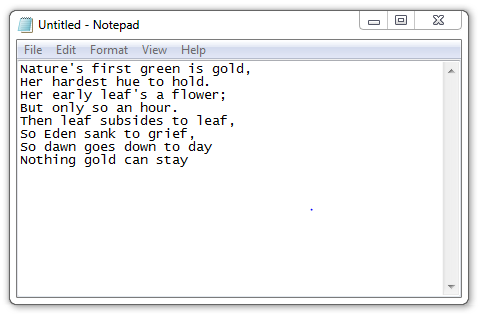
\includegraphics[width=0.85\textwidth]{Images/Chapter1/notepad.png}
        \caption{Notepad application for Windows 7.}
        \label{fig:ch1_notepad}
\end{figure}

A \acs{UI} that relies of visual cues, as the ones described above, is called a \ac{GUI}. The invention of such interfaces played a major role in the popularization of computers in the 80s. This is due to the fact that most users are more comfortable using such interfaces, as opposed to Command Line Interfaces (\acs{CLI}) that have been around since the late 60s.

In a \acs{CLI}, as opposed to an intuitive graphical interface, the user is presented with a \textbf{shell}\marginnotes{Shells are explained in Sections \ref{sec:ch1_terminology} and \ref{sec:ch1_sells}} prompt in which it can write commands to be interpreted by the \textbf{shell}. You can see an example below of a \acs{CLI} in which a user entered the command \textbf{\texttt{ls}} to list all files and folders in the working directory\marginnotes{In this book, the words \textbf{folder} and \textbf{directory} are used interchengeably}.

\begin{command_line}[Bash]
marcel@dell:~$ ls
Documents      Downloads      Pictures
Music          Video          seneca.pdf
marcel@dell:~$
\end{command_line}

In order to properly use a \acs{CLI}, the user needs to learn a series of commands that the shell understands, as well as the syntax of these commands. Hence, it should come to no surprise that most regular users prefer to use \acs{GUI}s which do not incur in such steep learning curves.

If you are reading this book, however, I expect you not to be a regular user. In fact, I expect you to be starting a career as systems analyst, a software developer, or other positions in the IT industry. For people like you, having a clear understanding of how to use a \acs{CLI} presents a number of advantages:
\begin{itemize}
    \item There are tasks that can only be achieved by using a \acs{CLI} because no \acs{GUI} has been created to perform them.
    \item Some tasks can be performed, using a \acs{CLI}, in a fraction of the time it would take using a \acs{GUI} tool.
    \item \acs{CLI}s can be accessed remotely in a fast and straightforward fashion, allowing you to control multiple systems from a single computer
    \item Users can quickly create scripts that run on \acs{CLI}s to automate repetitive tasks such as: adding new users to the system, backing up data, updating the system, etc.
    \item The steps required to perform some actions using \acs{GUI}s can vary a lot depending on which \acs{OS}, or Linux distribution, you are using. On the other hand, they are normally identical using a CLI. In fact, the same commands\marginnotes{With a few notable exceptions} can be used in all Linux distributions, Apple computers, and since 2016, even in Windows systems.
\end{itemize}

Most Linux distributions have a \acs{GUI} that allow regular users to achieve daily tasks such as web browsing, email, or writing documents. However, all Linux distributions also come with a terminal emulator that allow super users to do much more using a \acs{CLI}.

\section{Terminology}
\label{sec:ch1_terminology}

Before moving forward to learn how to use a Linux \acs{CLI}, It is important to notice the difference between three concepts that are often used interchangeably:

\begin{description}
\item[CLI] The \acs{CLI} is just the technical name of the method by which we interact with a computer by means of written instructions.
\item[Terminal] All major Linux distributions have a \acs{GUI}. However, they normally also provide you with a terminal, or more precisely a terminal emulator. A terminal emulator is nothing else than a program that provides us with a \acs{CLI} to interact with the \textbf{shell}.
\item[Shell] The \textbf{shell} is a software that reads keyboard commands and passes them to the \acs{OS} to carry out. Such commands could be used to perform simple tasks like listing the files in a particular folder, adding users to the system, creating folders, or complex tasks such as upgrading the \acs{OS}, installing applications, etc.
\end{description}


\section{Shells}
\label{sec:ch1_sells}

As mentioned before, a \textbf{shell} is a software that interprets commands passed by the user, and passes them to the \acs{OS}. However, just like there are multiple languages such as English, Spanish, or Mandarim, there are multiple shells available. Table~\ref{tab:ch1_shells} below presents a description of a few such shells\marginnotes{Many other shells exist, such as dash, ksh, etc}.

\begin{table}[!htbp]
   \myfloatalign
   \begin{tabularx}{\textwidth}{Xp{90mm}} \toprule
   %\tableheadline{Shell} & \tableheadline{Description}\\ \midrule
   \textbf{sh} & The Bourne shell, which has been distributed as the default \textbf{shell} for Unix since 1979. \\
   \textbf{bash} & Bourne Again Shell, an upgraded version of \textbf{sh}, written by the GNU Project, which has become the \textit{de facto} standard Linux shell. \\
   \textbf{csh} or \textbf{tcsh} & A Unix shell using a syntax similar to the \textbf{C} programming language. \textbf{tcsh} is identical to \textbf{csh}, with the addition of some extra features such as command-line completion.\\
   \bottomrule
   \end{tabularx}
\caption{Linux Shells}
\label{tab:ch1_shells}
\end{table}

In this book, we will cover exclusively the \textbf{bash shell}. This is due to the fact that \textbf{bash} is the default shell for the most widely used Linux distributions. In fact, it is hard to find a Linux distribution that does no come with a \textbf{bash shell}. That said, after learning how to use one shell, it is much easier to learn other shells, as they share many concepts and syntax.

\section*{Exercises}
\addcontentsline{toc}{section}{Exercises}

\begin{exercises}
   \item Explain, with your own words, what is a Command Line Interface (\acs{CLI}).
   \item Explain, with your own words, what is a Graphical User Interface (\acs{GUI}).
   \item What is the relationship between a terminal emulator, and a shell?
   \item Which commands are used to list all files in the working directory using the following shells: sh, bash, csh, dash, and ksh?
\end{exercises}

\chapter{Basic Shell Commands I}\label{ch:basic_commands}

In this chapter we will cover how to get access to a terminal emulator, as well as some very basic \textbf{bash} commands.

\section{Accessing a Terminal Emulator}

Once a user logs into a Linux \acs{OS} with a \acs{GUI}, there are multiple ways to get access to a \textbf{terminal emulator}. Some methods work only on a specific distribution, whereas some methods work on most distributions. In what follows, a list of methods to access terminal emulators are presented for some of the most popular desktop environments. The most commom Linux distribution for each desktop environment is presented in the margin notes.

\begin{description}
   \item[Gnome3] Press\marginpar{Debian, Red Hat, Fedora, CentOS, Kali} the super (windows) button to call the list of applications, and then type \textbf{\texttt{terminal}} in the search field, or search for the terminal in the provided applications list.
   \item[KDE] Click \marginpar{OpenSUSE, Kubuntu, Slackware} on the start button at the lower left, and then click on accessories, and finally on \textbf{\texttt{terminal}} .
   \item[Unity] Press\marginpar{Ubuntu} the super (windows) button to call the dash (or conversely click on the dash button at the upper left), and then type \textbf{\texttt{terminal}}.
\end{description}

In all of these desktop environments, the terminal emualtor can also be started by pressing \textbf{\texttt{crtl+alt+T}}.

\section{Terminal Basics}

Once the terminal emulator starts, the user is presented with an application displaying a blinking cursor at a \textbf{\texttt{shell prompt}}, just like shown bellow.

\begin{command_line}[Bash]
@@marcel@dell:~$@@
\end{command_line}

This prompt contain important information about the current parameters of the shell, namely: the username (\textbf{\texttt{marcel}}), system name (\textbf{\texttt{dell}}), and working directory (represented by a tilde [\textbf{\texttt{\texttildelow}}])\marginnotes{The \textbf{\texttt{\$}} separates command prompts from these current parameters}. A brief description of these parameters follows:

\begin{description}
\item [Username] Linux systems, as any Unix-like system, was designed to allow multiple users to access the system. When a terminal emulator starts, it assumes the user to be the same one that logged in into the GUI system. in Chapter \ref{ch:users_groups}, we will show how the \textbf{\texttt{su}} command can be used to switch users. In the example above, the username is \textbf{\texttt{marcel}}.

\item[System name] During the installation of Linux systems,  users are required to give your system (local machine) a name. When a terminal emulator starts, it assumes that you are using the local machine. In chapter XXX we will see how to log into remote machines using the \textbf{\texttt{ssh}} command. In the example above, my local machine is called is \textbf{\texttt{dell}}.

\item[Working directory] Imagine that you issue a command to create a file. In which directory will this file be created? The answer is: in the current \textbf{working directory}. When a terminal emulator starts, it assumes by default that you are at the home folder (directory) of the user currently logged in. Hence, whichever actions you perform will, by default, affect this directory. In Section \ref{sub:cd} , we will show how to use the \textbf{\texttt{cd}} command to change directories. In the example above, this home folder, which is located at \textbf{\texttt{/home/marcel}} is represented by a tilde (\textbf{\texttt{\texttildelow}}).
\end{description}

In what follows, a number of basic \textbf{\texttt{bash}}\marginnotes{You can easily switch shells by typing the name of the shell you want to switch to. For example, you can type \textbf{\texttt{dash}} to start using a \textbf{dash shell}} commands are presented.

\section{\textbf{\texttt{date}}}
To ask what day is today, you can type \textbf{\texttt{date}} \index{date} in the terminal emulator and press enter. The shell will verify the date with the \acs{OS}, display it in the terminal, and start a new prompt line ready to receive more commands, as shown below\marginnotes{For the following commands, we will ommit this new prompt line}. Note that the terminal also shows the current time and the time zone (Eastern Daylight Time - EDT).

\begin{command_line}[Bash]
@@marcel@dell:~$@@ date
Wed May 18 19:20:55 EDT 2016
@@marcel@dell:~$@@
\end{command_line}

Note that shell commands are \textbf{case-sensitive}. I.e., the shell diferentiates between upper-case and lower-case letters. For example, while \textbf{\texttt{date}} is a valid command, \textbf{\texttt{Date}} and \textbf{\texttt{DATE}} are not.

\section{\textbf{\texttt{whoami}}}
Not all terminal emulators display the username at each command prompt. Therefore, the shell needs to provide a method to verify the username of the current user. This is accomplished by the \textbf{\texttt{whoami}} (who am I) command, as shown below.

\begin{command_line}[Bash]
@@marcel@dell:~$@@ whoami
marcel
\end{command_line}

\section{\textbf{\texttt{pwd}}}
%The concept of a hyerarchical filesystem in which users can have create folders (directories) inside other folders was introduced with Unix. This concept is used by most modern OS, and Linux is no exception to this rule.

As mentioned before, when a terminal emulator is open, it needs a directory to act as a starting point. In most Linux system, this starting point is the user's home folder, located at \textbf{\texttt{/home/username}}, represented by a tilde (\textbf{\texttt{\texttildelow}}).

As we will show later, users can move to different directories using the shell. The shell's current location is called \textbf{working directory}. This is due to the fact that this is the directory that the shell will, by default, act (work) upon. In order to see in which directory you are currently at, you can type \textbf{\texttt{pwd}}\marginnotes{short for print working directory} in the terminal emulator and press enter. The shell will then print the working directory in the terminal, as shown below.

\begin{command_line}[C]
@@marcel@dell:~$@@ pwd
/home/marcel
\end{command_line}

\section{\textbf{\texttt{ls}}}
\label{sec:ls}

To obtain a list of all files and folders present in the working directory, as demonstrated in Chapter \ref{ch:cli_terminal_shell}, you can use the \textbf{\texttt{ls}}\marginnotes{short for list} command. The shell will then print a list of all files and folders, as shown below\marginnotes{Some terminal emulators use colours to distinguish between files, folders, scripts, etc}.

\begin{command_line}[Bash]
@@marcel@dell:~$@@ ls
Documents      Downloads      Pictures
Music          Video          seneca.pdf
\end{command_line}

The list command, by default, does not show hidden files\marginnotes{Hidden files are files whose names starts with a \textbf{\texttt{.}} (dot)}. In order to do so, you must add the option \textbf{\texttt{-a}} or \textbf{\texttt{--all}} to the ls command, as shown below:
\begin{command_line}[Bash]
@@marcel@dell:~$@@ ls
Documents      Downloads      Pictures
Music          Video          seneca.pdf
@@marcel@dell:~$@@ ls -a
.              ..             Documents
Downloads      Pictures       Music
Video          seneca.pdf     .System.conf
\end{command_line}
Note that in the command above, the file \textbf{\texttt{.System.conf}} only appears when the \textbf{\texttt{ls}} command is issued with the \textbf{\texttt{-a}} option. Also, note that two extra directories appear: a folder (\textbf{\texttt{.}}) and a folder (\textbf{\texttt{..}}). These are not real directories. They are simply hard links to the self (\textbf{\texttt{.}}) and parent (\textbf{\texttt{..}}) directories.

The list comand can also used to gather information about the files and folders in the current working directory. To do so, the \textbf{long list} option \textbf{\texttt{-l}} must be invoked, as shown below:
\begin{command_line}[Bash]
@@marcel@dell:~$@@ ls -a -l
drwxrwxr-x  3 marcel marcel  4096 Jun 21 23:06 .
drwxr-xr-x 54 marcel marcel  4096 Jun 21 18:59 ..
drwxrwxr-x  2 marcel marcel  4096 Jun 21 23:06 Documents
drwxrwxr-x  2 marcel marcel  4096 Jun 21 23:06 Downloads
drwxrwxr-x  2 marcel marcel  4096 Jun 21 23:06 Pictures
drwxrwxr-x  2 marcel marcel  4096 Jun 21 23:06 Music
drwxrwxr-x  2 marcel marcel  4096 Jun 21 23:06 Video
-rw-rw-r--  1 marcel marcel 12238 Jun 29 22:54 seneca.pdf
-rw-rw-r--  1 marcel marcel   126 Jun 28 20:52 .System.conf
\end{command_line}
This long list provides a number fo columns containing information about each file. In Table~ \ref{tab:ch2_list}, we explain what the information in each column represents using the file \textbf{\texttt{seneca.pdf}} as an example.

\begin{table}[!htbp]
   \myfloatalign
   \begin{tabularx}{\textwidth}{cXp{70mm}} \toprule
   %\tableheadline{Shell} & \tableheadline{Description}\\ \midrule
   \textbf{column} & \textbf{example} & \textbf{meaning} \\ \bottomrule
   \textbf{1} & \textbf{\texttt{-rw-rw-r--}} & File type and permission sets. These topics are covered in Chapter \ref{ch:users_groups}.\\
   \textbf{2} & \textbf{1} & Number of hard links to this file. Links are covered in Chapter \ref{ch:file_links}.\\
   \textbf{3} & \textbf{marcel} & Name of the user owner of the file. The concepts of users and ownership are covered in Chapter \ref{ch:users_groups}.\\
   \textbf{4} & \textbf{marcel} & Name of the group owner of the file. The concepts of groups and ownership are covered in Chapter \ref{ch:users_groups}.\\
   \textbf{5} & \textbf{12238} & Size of the file in bytes.\\
   \textbf{6} & \textbf{Jun 29 22:54} & Timestamp indicating when the file was edited for the last time.\\
   \textbf{7} & \textbf{seneca.pdf} & File name.\\
   \bottomrule
   \end{tabularx}
\caption{Long list information for the \textbf{\texttt{seneca.pdf}} file.}
\label{tab:ch2_list}
\end{table}

\section{\textbf{\texttt{tree}}}
The \mycommand{tree} command is somewhat similar to the \mycommand{ls} command. They both display a list of files and folders in the working directory. However, contrary to \mycommand{ls}, in which any subfolder is simply listed alongside files, the \mycommand{tree} command goes inside each subfolder and displays the files contained in them, creating a tree-like structure. See the example below:
\begin{command_line}
@@marcel@dell:Seneca$@@tree
.
|-- academic_honesty.pdf
|-- calendar.pdf
|-- OPS105
|   |-- students_list
|   |-- grades.xls
|-- SRT311
|   |-- students_list
|   |-- grades.xls

2 directories, 6 files
@@marcel@dell:Seneca$@@
\end{command_line}

The \mycommand{tree} command is not available by default in some Linux distributions. To install it, you must write the command \mycommand{sudo apt-get install tree}, and enter your user password.

\section{\textbf{\texttt{cd}}}
\label{sub:cd}
To switch working directories, you need only to use the \textbf{\texttt{cd}}\marginnotes{short for change directory} command, followed by the name of the directory you want to go. For example, assuming that the folders shown in the previous command's output do exist, typing \textbf{\texttt{cd Documents}} results in:
\begin{command_line}
@@marcel@dell:~$@@ pwd
/home/marcel
@@marcel@dell:~$@@ cd Documents
@@marcel@dell:Documents$@@ pwd
/home/marcel/Documents
\end{command_line}

The command \textbf{\texttt{cd}} by itself always sends the user back to the user's home folder. Also, the command \textbf{\texttt{cd ..}} sends the user to the parent folder of the working directory, and the command \textbf{\texttt{cd -}} sends the user back to the previous working directory. The parent folder is the folder hierarchically above the current folder. For example, the folder \textbf{\texttt{/home/marcel}} is the parent folder of \textbf{\texttt{/home/marcel/Documents}}.

Finally, note that if you enter the name of a directory that does not exist, the shell will return an error message and then it will start a new prompt line ready to receive more commands, as shown next.

\begin{command_line}[make]
@@marcel@dell:~$@@ cd DOCUMENTS
bash: cd: DOCUMENTS: No such file or directory
@@marcel@dell:~$@@
\end{command_line}

\section{Relative and Absolute Paths}

In our previous example using the \textbf{\texttt{cd}} command, we switched working directories from one folder, \textbf{\texttt{/home/marcel}}, to one of its immediate subfolders, \textbf{\texttt{/home/marcel/Documents}}. However, you might face more complex situations in which you have a directory tree as shown in Figure \ref{fig:ch2_dirtree}, and you want to switch the current working directory from any folder directly to any other folder.

\begin{figure}[!htbp]
  \centering
        \tikzstyle{every node}=[thick,anchor=west, font={\scriptsize\ttfamily}, inner sep=2.5pt]
\tikzstyle{selected}=[draw=black]
\tikzstyle{root}=[selected, fill=black!20]

\begin{tikzpicture}[%
    scale=.99,
    grow via three points={one child at (0.5,-0.65) and
    two children at (0.5,-0.65) and (0.5,-1.1)},
    edge from parent path={(\tikzparentnode.south) |- (\tikzchildnode.west)}]
  \node [root] {/}
    child { node [selected] {home}
      child { node [selected] {marcel}
        child { node [selected] {Seneca}
           child { node {ops105.sh}}
           child { node {srt311.py}}
        }
        child { node at (0, -2.0) [selected] {Personal}
           child { node {bills.doc}}
           child { node {summer.jpg}}
        }
      }
    }
    child { node at (0,-5.0) [selected] {media}
      child { node [selected] {Seneca}
        child { node {bts490.c}}
        child { node {btn415.cpp}}
      }
    }
    child { node at (0,-7.0) {\dots}};
\end{tikzpicture}

        \caption{Directory tree.}
        \label{fig:ch2_dirtree}
\end{figure}

For example, given the directory tree shown in Figure \ref{fig:ch2_dirtree}, how can we directly switch working directories for the following cases:
\begin{itemize}
\item from \textbf{\texttt{/home}} directly to \textbf{\texttt{/home/marcel/Personal}}
\item from \textbf{\texttt{/home/marcel/Seneca}} directly to \textbf{\texttt{/media}}
\item from \textbf{\texttt{/home/marcel/Seneca}} to \textbf{\texttt{/media/Seneca}}
\end{itemize}
The solution to all these cases is: ``by providing either a \textbf{relative path} or an \textbf{absolute path} to the desired folders.'' In what follows, we define these two concepts\marginnotes{Note that the concepts of relative and absolute paths also apply to files}.

\subsection{Relative Path}
 When a relative path is provided, the shell assumes that the starting point of the path is the current working directory. For example, given that you are currently in \textbf{\texttt{/home}}, you can switch your working directory to \textbf{\texttt{/home/marcel/Personal}} by issuing the command: \textbf{\texttt{cd marcel/Personal}}, as shown in what follows.
\begin{command_line}
@@marcel@dell:home$@@ pwd
/home
@@marcel@dell:home$@@ cd marcel/Personal
@@marcel@dell:Personal$@@ pwd
/home/marcel/Personal
\end{command_line}
\subsection{Absolute Path}
 Absolute paths always start with \textbf{\texttt{/}}\marginnotes{\textbf{\texttt{/}} denotes the root, of all directories in a Linux system} and provide the complete path for the desired folder or file. For example, given that your working directory is \textbf{\texttt{/home/marcel/Seneca}}, you can switch to \textbf{\texttt{/media}} by issuing the command: \textbf{\texttt{cd /media}}, or you can switch  to \textbf{\texttt{/media/Seneca}} by issuing the command: \textbf{\texttt{cd /media/Seneca}} , as shown in what follows.
\begin{command_line}
@@marcel@dell:Seneca$@@ pwd
/home/marcel/Seneca
@@marcel@dell:Seneca$@@ cd /media
@@marcel@dell:media$@@ pwd
/media
\end{command_line}
\begin{command_line}
@@marcel@dell:Seneca$@@ pwd
/home/marcel/Seneca
@@marcel@dell:Seneca$@@ cd /media/Seneca
@@marcel@dell:Seneca$@@ pwd
/media/Seneca
\end{command_line}

Relative and absolute paths can be compared to addresses in navigation systems. For example, if you live in Toronto, and you want to go to a place within the city, you can type on your navigation device an address such as 200 King Street. The device will assume that this address is in Toronto-ON, Canada. This would be the compared to a relative address, as the starting point is assumed to be the city of Toronto. However, if you are in Toronto and you want to go to 200 King Street in Buffalo-NY, you would need to enter the complete address, including the city, state, and sometimes even the country. This would be compared to an absolute value, as the address is completely defined.

\section{\textbf{\texttt{clear}}}

All commands you enter, as well as their outputs, stay in the screen and you are given a new shell prompt at the bottom to keep working with the shell. This can lead to a very polluted screen containing a lot of information that is no longer necessary.

In order to clear the screen from all previous commands and ouputs, you simple have to issue the \textbf{\texttt{clear}} command. This command will erase from your terminal all information in it and provide you with a command prompt at the top to keep working with the shell.

It is important to note that this command simply clears the terminal display. Any variables\marginnotes{Variables are covered in Chapter~\ref{ch:intro_scripting}} that have been defined, or any modifications to the state of the shell will not be changed by this command.

\section{Command History}

You can use the up ($\uparrow$) and down ($\downarrow$) arrow keys in order to navigate the commands you have previously entered in your shell. For example, by hitting the up arrow key once, you will get the previously entered command. Hitting the up arrow again, will get you the command you entered prior to that one.

\section*{Exercises}
\addcontentsline{toc}{section}{Exercises}

\begin{exercises}
   \item Describe two methods to open a terminal emulator on a Ubuntu Linux OS.
   \item Given the command prompt below, who is the user currently logged into the shell? Also, what is the name of the local machine? Finally, what is the current working directory?
\begin{command_line}
@@john@lenovo:~$@@
\end{command_line}
   \item What is the relationship between a \textbf{terminal emulator}, and a \textbf{shell}?
   \item Which commands are used to list all files in the working directory using the following shells: bash, csh, dash, and ksh?
   \item Which command can be used to show in the terminal what time is it?
   \item What is the output of the \textbf{\texttt{ls -l}} command? What does the 6$^{\text{th}}$ column represents?
   \item How can you move back to the latest previously accessed working directory using only one shell command?
   \item What happens when you apply the parent folder parameter to the \textbf{\texttt{cd}} command twice. In other words, what happens when you issue a \textbf{\texttt{cd ../..}} command?

Given the directory tree shown in Figure \ref{fig:ch2_ex_dirtree} (on next page), answer the following questions:
\begin{figure}[!htbp]
  \centering
        \tikzstyle{every node}=[thick,anchor=west, font={\scriptsize\ttfamily}, inner sep=2.5pt]
\tikzstyle{selected}=[draw=black]
\tikzstyle{root}=[selected, fill=black!20]

\begin{tikzpicture}[%
    scale=.99,
    grow via three points={one child at (0.5,-0.65) and
    two children at (0.5,-0.65) and (0.5,-1.1)},
    edge from parent path={(\tikzparentnode.south) |- (\tikzchildnode.west)}]
  \node [root] {/}
    child { node [selected] {home}
      child { node [selected] {marcel}
          child { node {ops105.sh}}
          child { node {srt311.py}}
        }
      }
    child { node at (0,-2.0) [selected] {media}
      child { node [selected] {Seneca}
        child { node {bts490.c}}
        child { node {btn415.cpp}}
      }
    }
    child { node at (0,-4.0) {\dots}};
\end{tikzpicture}

        \caption{Directory tree for questions 9, 10, and 11.}
        \label{fig:ch2_ex_dirtree}
\end{figure}
   \item Write a command to switch your working directory from \textbf{marcel} to \textbf{Seneca} using only one shell command?
   \item Write a command to switch your working directory from \textbf{media} to \textbf{marcel} using only one shell command.
   \item Given that your working directory is \textbf{media}, can you use a relative path to move to \textbf{Seneca}? If yes, can you also use an absolute path? Which one of these options seem more appropriate in this case?
\end{exercises}

\chapter{Basic Shell Commands II}\label{ch:basic_commands_ii}

In our previous chapter, we covered a number of bash commands which could be used to: gather information from the system and user (\textbf{\texttt{date}},  \textbf{\texttt{whoami}}, \textbf{\texttt{pwd}}), get information about files and folders (\textbf{\texttt{ls}}), or to change de current working directory (\textbf{\texttt{cd}}).

None of the commands could be used to alter files, folders, or change the configurations of the system, though. I.e., they have no lasting effect in the system.

In this chapter, we will cover a series of commands that have lasting effects in files, folders, and possibly the system. The commands we are covering in this chapter can be used to create and remove files and folders, as well as to rename and make copies of them.

\section{\textbf{\texttt{mkdir}}}

To create new folders, the \textbf{\texttt{mkdir}}\marginnotes{short for make directory} command can be used, followed by the name(s) of the folder(s) to be created. In the example below, a folder called \textbf{Samples} is created in the current working directory.

\begin{command_line}[Bash]
@@marcel@dell:~$@@ ls
Documents      Downloads      Pictures
Music          Video          seneca.pdf
@@marcel@dell:~$@@ mkdir Samples
@@marcel@dell:~$@@ ls
Documents      Downloads      Pictures    @@Samples@@
Music          Video          seneca.pdf
\end{command_line}

Note that, by default, the new directory is created as a subfolder of the working directory. To create folders in other locations, without leaving the current working directory, you can use the \textbf{\texttt{mkdir}} command combined with relative or absolute paths, as shown below:

\begin{command_line}[Bash]
@@marcel@dell:~$@@ ls Documents
Seneca      Personal
@@marcel@dell:~$@@ mkdir ~/Documents/Samples
@@marcel@dell:~$@@ ls Documents
Seneca      Personal    @@Samples@@
\end{command_line}

\begin{my_box}[Files and Folders with spaces in their names]
  In all examples that were given so far is this book, all files and folders do not contain spaces in their names. Issuing a command such as \textbf{\texttt{mkdir My Documents}} would create two folders, one called \textbf{\texttt{My}} and another called \textbf{\texttt{Documents}}. This is because the shell cannot distinguish between an argument with a space, or two arguments without spaces.

  Linux can handle files and folder with spaces, though. In order to do so, whenever you are refering to a file or folder with sapces in its name, each space needs to be preceeded by a backslash (\textbf{\texttt{\textbackslash}}). For example, you can create a folder called \textbf{\texttt{My Documents}} by issuing a command \textbf{\texttt{mkdir My\textbackslash Documents}}.
\end{my_box}


\section{\textbf{\texttt{rmdir}}}

The \textbf{\texttt{rmdir}}\marginnotes{short for remove directory} command, as the name suggests, deletes existing folders. For example, \textbf{\texttt{rmdir Samples}} will remove a folder \textbf{\texttt{Samples}} from the current working directory. It is important to note that it can only be used to remove empty folders. In case the folder is not empty, the shell returns an error message.

In the example below, the \textbf{\texttt{rmdir}} command is applied to both an empty folder \textbf{Samples}, and to a non-empty folder \textbf{Pictures}.
\begin{command_line}[Bash]
@@marcel@dell:~$@@ ls
Documents      Downloads      Pictures    @@Samples@@
Music          Video          seneca.pdf
@@marcel@dell:~$@@ rmdir Samples
@@marcel@dell:~$@@ ls
Documents      Downloads      Pictures    Music
Video          seneca.pdf
@@marcel@dell:~$@@ rmdir Pictures
rmdir: failed to remove 'Pictures': Directory not empty
@@marcel@dell:~$@@
\end{command_line}

\section{\textbf{\texttt{touch}}}

As shown in Section \ref{sec:ls}, files and folders in Linux have a timestamp indicating when they were edited for the last time. The \textbf{\texttt{touch}} command, when applied to an existing file, updates the timestamp of when it was last edited\marginnotes{Updated timestamps are useful for some backup programs, among other uses}. It is equivalent to opening the file, saving it, and then closing it. As an example, see the command prompt below:
\begin{command_line}[Bash]
@@marcel@dell:~$@@ ls -l
total 0
-rw-rw-r-- 1 marcel marcel 0 Jul 12 11:31 final_exam.doc
-rw-rw-r-- 1 marcel marcel 0 Jun 21 20:30 introduction.ppt
-rw-rw-r-- 1 marcel marcel 0 May 10 21:41 seneca.pdf
@@marcel@dell:~$@@ touch final_exam.doc
@@marcel@dell:~$@@ ls -l
total 0
-rw-rw-r-- 1 marcel marcel 0 @@Jul 14 22:12@@ final_exam.doc
-rw-rw-r-- 1 marcel marcel 0 Jun 21 20:30 introduction.ppt
-rw-rw-r-- 1 marcel marcel 0 May 10 21:41 seneca.pdf
\end{command_line}
When applied to non-existing files, the \textbf{\texttt{touch}} command creates empty files, as shown below:
\begin{command_line}[Bash]
@@marcel@dell:~$@@ ls -l
total 0
-rw-rw-r-- 1 marcel marcel 0 Jul 14 22:12 final_exam.doc
-rw-rw-r-- 1 marcel marcel 0 Jun 21 20:30 introduction.ppt
-rw-rw-r-- 1 marcel marcel 0 May 10 21:41 seneca.pdf
@@marcel@dell:~$@@ touch mid_term.doc
@@marcel@dell:~$@@ ls -l
total 0
-rw-rw-r-- 1 marcel marcel 0 Jul 14 22:12 final_exam.doc
-rw-rw-r-- 1 marcel marcel 0 Jun 21 20:30 introduction.ppt
-rw-rw-r-- 1 marcel marcel 0 May 10 21:41 seneca.pdf
@@-rw-rw-r-- 1 marcel marcel 0 Jul 14 22:15 mid_term.doc@@
\end{command_line}
This second usage of the \textbf{\texttt{touch}} command is frequently used for testing purposes\marginnotes{tip: you to use \textbf{\texttt{touch}} and \textbf{\texttt{mkdir}} in order to recreate the examples provided in this chapter.}.

\section{\textbf{\texttt{rm}}}

To delete (remove) files, the \textbf{\texttt{rm}}\marginnotes{short for remove} command can be used, followed by the name(s) of file(s) to be deleted from the working directory. See the example below:

\begin{command_line}[Bash]
@@marcel@dell:~$@@ ls
Documents      Downloads      Pictures
Music          Video          @@seneca.pdf@@
@@marcel@dell:~$@@ rm seneca.pdf
@@marcel@dell:~$@@ ls
Documents      Downloads      Pictures
Music          Video
\end{command_line}

The \textbf{\texttt{rm}} command can also be used to remove non-empty folders. To do so, we have to apply the \textbf{\texttt{-r}} (recursive) option followed by the name of the folder, as shown below.
\begin{command_line}[Bash]
@@marcel@dell:~$@@ ls
Documents      Downloads      @@Pictures@@
Music          Video          seneca.pdf
@@marcel@dell:~$@@ rm -r Pictures
@@marcel@dell:~$@@ ls
Documents      Downloads      Music
Video          seneca.pdf
\end{command_line}

%It is important to note that, by default, this command does not ask for confirmation, prior to deleting the file. Also, most Linux distributions do not have a recycle being. Hence, it is important to be careful before using this command.

\begin{my_box}[Bash Design Goals]
  It is important to note that the commands described in this chapter don't normally ask for confirmation. For example, when deleting a file using the \textbf{\texttt{rm}} command, the \textbf{shell} will not ask the user if he/she is sure he/she wants to delete the file. Nor the file will be sent to a recycle bin from which it can be recovered. The file will simply be deleted.

  The \textbf{shell} performs tasks that might incur in unforeseen consequences, such as accidently deleting a number of files, in a much more direct way because of its design goals. As opposed to \acs{GUI} interfaces where the goal normally is to provide a platform for inexperienced users to perform basic tasks, a \acs{CLI} is normally designed with the goal of allowing experienced users to quickly perform complex tasks.
\end{my_box}

\section{\textbf{\texttt{mv}}}

The \textbf{\texttt{mv}}\marginnotes{short for move} command can be used in two distinct ways. As the name suggests, it can move a file, a folder, or a number of files and folders from one directory to another. However, it can also be used to rename single files or folders. Both uses of this command are described in what follows.

\subsection{Moving files and folders accross directories}

To move a single file from one directory to another, the \textbf{\texttt{mv}} command needs two arguments. The first being the name of the file in the working directory to be moved, and the second being the absolute or relative path of the directory we are moving the file to. See the example below:
\begin{command_line}[Bash]
@@marcel@dell:~$@@ ls
@@final_exam.doc@@  introduction.ppt  seneca.pdf
Folder
@@marcel@dell:~$@@ mv final_exam.doc Folder
@@marcel@dell:~$@@ ls
introduction.ppt  seneca.pdf  Folder
@@marcel@dell:~$@@ ls Folder
@@final_exam.doc@@
@@marcel@dell:~$@@
\end{command_line}

Note that, in this example, the file \textbf{final\_exam.doc} disappears from the working directory and appears in the \textbf{Folder} directory.

Multiple files can be moved with a single \textbf{\texttt{mv}} command. To do so, you first need to provide the names of all files you intend to move as arguments. Then, you need to provide the relative or absolute path of the directory you want to move them to as the very last argument. This technique is  shown in what follows:
\begin{command_line}[Bash]
@@marcel@dell:~$@@ ls
@@final_exam.doc@@  @@introduction.ppt@@  seneca.pdf
Folder
@@marcel@dell:~$@@ mv final_exam.doc introduction.ppt Folder
@@marcel@dell:~$@@ ls
seneca.pdf  Folder
@@marcel@dell:~$@@ ls Folder
@@final_exam.doc@@ @@introduction.ppt@@
@@marcel@dell:~$@@
\end{command_line}

Note that, within this context, this command can also be applied to folders (directories). I.e., you can move an entire folder in your working directory into other folders using the exactly same syntax applied for files in this section.

\subsection{Renaming files and folders}

Imagine the \textbf{\texttt{mv}} command being used with two arguments, the first being a file name in the working directory, and the second being a name that doesn't match any directories. In this scenario, the \textbf{\texttt{mv}} command will rename the file indicated by the first argument to the name specified in the second\marginnotes{A command called \textbf{\texttt{rename}} exists in \textbf{\texttt{bash}}. However, it is used to rename multiple files at once using regular expressions. Regular expressions are covered in Chapter~\ref{ch:grep}}. See the example below:
\begin{command_line}[Bash]
@@marcel@dell:~$@@ ls
@@final_exam.doc@@  introduction.ppt  seneca.pdf
Folder
@@marcel@dell:~$@@ mv final_exam.doc final_exam_fall.doc
@@marcel@dell:~$@@ ls
@@final_exam_fall.doc@@  introduction.ppt  seneca.pdf
Folder
@@marcel@dell:~$@@
\end{command_line}
In this example, you can see that the file \textbf{final\_exam.doc} was renamed to \textbf{final\_exam\_fall.doc}.

You can also rename a folder using the same syntax applied for files in this section.

\section{\textbf{\texttt{cp}}}

The \textbf{\texttt{cp}}\marginnotes{short for copy} command can be used to copy files and folders. It can be used in two distinct ways:


\subsection{Copying files within the working directory}

To create a copy of a file in the same working direct, the \textbf{\texttt{cp}} command should be used with two arguments. The first argument should be the name of the file to be copied, while the second argument should be the name of the copy, as shown below:
\begin{command_line}[Bash]
@@marcel@dell:~$@@ ls
final_exam.doc  introduction.ppt  seneca.pdf
Folder
@@marcel@dell:~$@@ cp final_exam.doc final_exam_fall.doc
@@marcel@dell:~$@@ ls
final_exam.doc  @@final_exam_fall.doc@@  introduction.ppt
seneca.pdf  Folder
@@marcel@dell:~$@@
\end{command_line}

To copy an entire folder in your working directory into another folder also in the working directory, you must use the recursive option \textbf{\texttt{-r}}, as shown in the example below:
\begin{command_line}[Bash]
@@marcel@dell:~$@@ ls
final_exam.doc  introduction.ppt  seneca.pdf
Folder
@@marcel@dell:~$@@ cp -r Folder Folder_Copy
@@marcel@dell:~$@@ ls
final_exam.doc  final_exam_fall.doc  introduction.ppt
seneca.pdf  Folder  @@Folder_Copy@@
@@marcel@dell:~$@@
\end{command_line}

\subsection{Copying files to other directories}

To create a copy of a file in the working directory to another directory, the second argument of the \textbf{\texttt{cp}} command must be the absolute or relative path of the directory in which you want to plae a copy of the file. In this case, the new file will have the same name as the original file. See the example below:
\begin{command_line}[Bash]
@@marcel@dell:~$@@ ls
final_exam.doc  introduction.ppt  seneca.pdf
Folder
@@marcel@dell:~$@@ cp final_exam.doc Folder
@@marcel@dell:~$@@ ls
final_exam.doc  introduction.ppt  seneca.pdf
@@Folder@@
@@marcel@dell:~$@@ ls Folder
@@marcel@dell:~$@@ ls
final_exam.doc
@@marcel@dell:~$@@
\end{command_line}

Just as with the previous scenario, to copy an entire folder in the working directory to another directory, you also must use the recursive option \textbf{\texttt{-r}}. See the example below:
\begin{command_line}[Bash]
@@marcel@dell:~$@@ ls
final_exam.doc  introduction.ppt  seneca.pdf
Folder  Music
@@marcel@dell:~$@@ cp Music Folder
cp: omitting directory 'Music'
@@marcel@dell:~$@@ ls Folder
final_exam.doc  introduction.ppt
@@marcel@dell:~$@@ cp -r Music Folder
@@marcel@dell:~$@@ ls Folder
final_exam.doc  introduction.ppt  @@Music@@
@@marcel@dell:~$@@
\end{command_line}

To copy all contents of a folder to another folder, but not the folder itself, you need to add \textbf{\texttt{/.}} to the end of the name of the folder you are copying, as shown below\marginnotes{You can also use this technique with the \textbf{\texttt{mv}} command}:
\begin{command_line}[Bash]
@@marcel@dell:~$@@ ls
final_exam.doc  introduction.ppt  seneca.pdf
Folder  Music
@@marcel@dell:~$@@ cp -r Music/. Folder
@@marcel@dell:~$@@ ls Folder
arcade_fire-ready_to_start.mp3  foo_fighters-walk.mp3
@@marcel@dell:~$@@
\end{command_line}


\section*{Exercises}
\addcontentsline{toc}{section}{Exercises}

\begin{exercises}
   \item What is the main difference between using the copy \textbf{\texttt{cp}}, and the move \textbf{\texttt{mv}} commands, when applied to files?
   \item How can you delete a non-empty folder called \textbf{Archive} that exists in your working directory?
   \item Which command can be used to move a file called \textbf{README.txt} from your working directory to its parent folder
   \item Which command can be used to create a folder called \textbf{Examples} inside a subfolder called \textbf{Documentation} that exists in your working directory. See the diagram in Figure \ref{fig:ch3_dirtree}.
   \begin{figure}[!htbp]
     \centering
           \tikzstyle{every node}=[thick,anchor=west, font={\scriptsize\ttfamily}, inner sep=2.5pt]
\tikzstyle{selected}=[draw=black]
\tikzstyle{created}=[draw=gray,dashed]
\tikzstyle{root}=[selected, fill=black!20]

\begin{tikzpicture}[%
    scale=.99,
    grow via three points={one child at (0.5,-0.65) and
    two children at (0.5,-0.65) and (0.5,-1.1)},
    edge from parent path={(\tikzparentnode.south) |- (\tikzchildnode.west)}]
  \node [root] {/}
    child { node [selected] {home}
      child { node [selected] {marcel}
        child { node [selected] {Documentation}
           child { node [created] {Examples}}
           child { node {Example1.txt}}
           child { node {Example2.txt}}
        }
        child { node at (0, -2.0) [selected] {Personal}
           child { node {bills.doc}}
           child { node {summer.jpg}}
        }
      }
    }
    child { node at (0,-5.0) {\dots}};
\end{tikzpicture}

           \caption{Directory tree for questions 4 and 5.}
           \label{fig:ch3_dirtree}
   \end{figure}
   \item Still with regards to the diagram diagram in Figure \ref{fig:ch3_dirtree}, how can you move files \textbf{Example1.txt} and \textbf{Example2.txt} from the \textbf{Documentation} folder to its \textbf{Examples} subfolder, without changing your working directory.
   \item Is it possible to delete multiple empty folders with only one \textbf{\texttt{rmdir}} command? If so, how can you delete two empty folders named \textbf{Tests} and \textbf{Assignments} from your working directory?
   \item What happens when you apply the \textbf{\texttt{touch}} command to an existing file? Also, what happens when you apply this command to a non-existing file.
   \item How can you make copies of the contents of a file called \textbf{exams.txt} from your working directory, to a file called \textbf{exams.txt} inside a subfolder \textbf{Classes} that exists in your working directory?
   \item What happens when the first parameter of a \textbf{\texttt{mv}} command is a file, and the second parameter is a folder?
   \item Which command can be used to copy the contents of a subfolder named \textbf{Folder1}, that exists in the current working directory, to another subfolder named  \textbf{Folder1Copy} in the same working directory. Note that the subfolder \textbf{Folder1Copy} doesn't exist prior to the command you need to enter.
\end{exercises}

%************************************************
\chapter{Getting Help}\label{ch:getting_help}
%************************************************
We have already covered in previous chapters a number of commands which can take multiple options and different numbers of arguments. For example, it was shown in Chapter \ref{ch:basic_commands} that the command \textbf{\texttt{ls}} can work in three different ways:

\begin{itemize}
  \item By itself, this command prints the names of all files in the working directory.
  \item When provided with the name of another folder as an argument, this command prints the names of all files in the specified folder.
  \item If called with the the option \textbf{\texttt{-l}}\marginnotes{There are many more options for the \textbf{\texttt{ls}} command.}, this command gives all the information about files described on Table \ref{tab:ch2_list}, as opposed to just listing their names.
\end{itemize}

The bash shell has hundreds of commands like \textbf{\texttt{ls}} that can take multiple options and different numbers of arguments. Hence, in order to be accessible to non-experts, it needs to provide its users with a way of knowing how to use those commands.

In this chapter we will cover different ways in which users can get help on how to use different commands.

\section{\textbf{\texttt{help}}}

By itself, the \textbf{\texttt{help}} command will list all \textbf{built-in}\marginnotes{Built-in commands are explained in the Built-in Commands box that follows} commands. If one of the built-in commands is provided as an argument, this command provides a quick description of the provided command, and possibly a list of options. You can see below the output of entering \textbf{\texttt{help pwd}} on bash.

\begin{command_line}[make]
@@marcel@dell:~$@@ help pwd
pwd: pwd [-LP]
    Print the name of the current working directory.

    Options:
      -L	print the value of $PWD if it names the current working directory
      -P	print the physical directory, without any symbolic links

    By default, 'pwd' behaves as if '-L' were specified.

    Exit Status:
    Returns 0 unless an invalid option is given or the current directory cannot be read.\end{command_line}

Note that \textbf{\texttt{help}} only covers built-in commands. It does not cover commands implemented as binary files in \textbf{/bin} or \textbf{/usr/bin}, such as \textbf{\texttt{ls}}, \textbf{\texttt{rm}}, \textbf{\texttt{mv}}, and many others.


\begin{my_box}[Built-in Commands]
  Most commands in bash, such as \textbf{\texttt{ls}}, \textbf{\texttt{rm}}, and \textbf{\texttt{touch}} are implemented by binary files located in the \textbf{/bin} and \textbf{/usr/bin} folders. These commands are interpreted in the same way as any other application the shell can run. I.e., the shell asks the kernel to execute it, and after it has finished executing, the shell receives its output.

  Built-in commands, on the other hand, are an integral part of the shell. They are not implemented in a separated file. The main reason why some commands are implemented directly inside the shell is because they need to change the state of the shell. For example, the \textbf{\texttt{cd}} command is a built-in command because it changes the current working directory. Commands implemented as binaries, such as \textbf{\texttt{ls}}, \textbf{\texttt{rm}}, and \textbf{\texttt{touch}}, cannot change the state of the shell.

  Another reason for implementing some commands directly into the shell is because it normally enhances their performance.
\end{my_box}

\section{\textbf{\texttt{man}}}

Since the inception of Unix, it has become standard practice for the authors of scripts that implement shell commands to provide manual pages for them. This practice was continued by the GNU project when rewritting Unix as an open source project\marginnotes{In fact, the author of the manual pages for many basic commands such as \textbf{\texttt{ls}} and \textbf{\texttt{rm}} is no one less than Richard Stallman, the programmer that started the GNU project, as discussed in Chapter~\ref{ch:history}}.

All manual pages follow the same structure show in Listing \ref{lst:mkdir_man} (page \pageref{lst:mkdir_man}). I.e., they have the following sections:

\begin{source_code_float}{make}{Manual page for the \textbf{\texttt{mkdir}} command.}{lst:mkdir_man}
  MKDIR(1)            User Commands               MKDIR(1)

  NAME
         mkdir - make directories
  SYNOPSIS
         mkdir [OPTION]... DIRECTORY...
  DESCRIPTION
         Create the DIRECTORY(ies), if they do not already exist.
         Mandatory arguments to long options are mandatory for short options too.

         -m, --mode=MODE
            set file mode (as in chmod), not a=rwx - umask
         -p, --parents
                no error if existing, make parent directories as needed
         -v, --verbose
                print a message for each created directory
         -Z     set SELinux security context of each created directory to the default type
         --context[=CTX]
                like -Z, or if CTX is specified then set the SELinux or SMACK security context to CTX
         --help   display this help and exit
         --version   output version information and exit
  AUTHOR
         Written by David MacKenzie.
  REPORTING BUGS
         GNU coreutils online help: <http://www.gnu.org/software/coreutils/>
         Report mkdir translation bugs to <http://translationproject.org/team/>
  COPYRIGHT
         Copyright 2014 Free Software Foundation, Inc.  License GPLv3+: GNU GPL version 3 or later <http://gnu.org/licenses/gpl.html>.
         This  is free software: you are free to change and redistribute it.  There is NO WARRANTY, to the extent permitted by law.
  SEE ALSO    mkdir(2)

         Full documentation at: <http://www.gnu.org/software/coreutils/mkdir> or available locally via: info '(coreutils) mkdir invocation'

  GNU coreutils 8.23    November 2015    MKDIR(1)\end{source_code_float}

\begin{description}
\item{\textbf{Name}} States the name and purpose of the command
\item{\textbf{Synopsis}} Briefly describes the command syntax
\item{\textbf{Description}} Describes the command as well as its options
\item{\textbf{Authors}} Lists the authors of the script that implements the command
\item{\textbf{Reporting Bugs}} Provides a link to a page where bugs can be reported
\item{\textbf{Copyright}} States that the code is provided as free software
\item{\textbf{See Also}} Provides a list of related commands
\end{description}

To access manual pages, you need only to use the \textbf{\texttt{man}} command, followed by the name of the command you are trying to get information about.\marginnotes{Manual pages cover not only commands, but also daemons and config files}. See the example below:

\begin{command_line}[Bash]
@@marcel@dell:~$@@ man mkdir
\end{command_line}

\subsection{Sections}

Note that the \textbf{\texttt{mkdir}} command appears with a \textbf{\texttt{(1)}} next to it at the top of Listing \ref{lst:mkdir_man} (see page  \pageref{lst:mkdir_man}). This number denotes the section of the manual from where the information was retrieved. Some commands have the same name of \textbf{deamons} or \textbf{config files}. Hence, dividing manual pages in sections makes it possible for users to access the manual page for the right tool. Manual pages are divided in 9 sections, as shown in Table \ref{tab:man_sections}.

\begin{table}[!htbp]
   \myfloatalign
   \begin{tabularx}{\textwidth}{Xp{105mm}} \toprule
   \textbf{1} & Executable programs or shell commands \\
    \textbf{2} & System calls (functions provided by the kernel) \\
   \textbf{3} & Library calls (functions within program libraries) \\
   \textbf{4} & Special files (usually found in \textbf{\texttt{/dev}})\\
   \textbf{5} & File formats and conventions e.g. \textbf{\texttt{/etc/passwd}}\\
   \textbf{6} & Games\\
   \textbf{7} & Miscellaneous (including macro packages and conventions), e.g. man(7), groff(7) \\
   \textbf{8} & System administration commands (usually only for root)\\
   \textbf{9} & Kernel routines [Non standard] \\
   \bottomrule
   \end{tabularx}
\caption{Manual Page Sections}
\label{tab:man_sections}
\end{table}

By default, \textbf{\texttt{man COMMAND}} retrieves the first occurrence of \textbf{\texttt{COMMAND}} in the manual pages. In order to access later occurrences, you need to provide the section as the first argument followed by the name of the command. For example, \textbf{\texttt{passwd}} is both a command, as well as a config file. To access the manual for the \textbf{\texttt{passwd}} command, one can write:
\begin{command_line}[Bash]
@@marcel@dell:~$@@ man passwd
\end{command_line}
or
\begin{command_line}[Bash]
@@marcel@dell:~$@@ man 1 passwd
\end{command_line}

However, to access the \textbf{\texttt{passwd}} config page manual, one needs to write:
\begin{command_line}[Bash]
@@marcel@dell:~$@@ man 5 passwd
\end{command_line}

\section{\textbf{\texttt{whatis}}}

As shown in Listing \ref{lst:mkdir_man}, each manual page comes with a description section. The \textbf{\texttt{whatis}} command searches the man page of the command provided as an argument and displays its description. See the example below:
\begin{command_line}[Bash]
@@marcel@dell:~$@@ whatis ls
ls (1)               - list directory contents
\end{command_line}
If the argument can be found in multiple sections, all descriptions are provided in the output, as shown below:
\begin{command_line}[Bash]
@@marcel@dell:~$@@ whatis passwd
passwd (1)           - change user password
passwd (5)           - the password file
\end{command_line}


\section{\textbf{\texttt{apropos}}}

In English, the word apropos means: \textit{concerning, with reference to}. The \textbf{\texttt{apropos}} command is called using keywords as arguments. It returns a single line for each man page that contains one or more of the keyword(s) in its \textbf{NAME} section.

This command comes handy when you need to search for commands which names you are not certain of. See the example below\marginnotes{A few extra outputs from this command were ommited for simplicity}:

\begin{command_line}[Bash]
@@marcel@dell:~$@@ apropos rename
dpkg-name (1) - rename Debian packages to full package names
mv (1)        - move (rename) files
rename (1)    - renames multiple files
rename (2)    - change the name or location of a file
renameat (2)  - change the name or location of a file
\end{command_line}
In this example you can see that the \textbf{\texttt{mv}} command can be used to rename a single file, while the \textbf{\texttt{rename}} command is normally only used to rename multiple files at once.

\section{\textbf{\texttt{info}}}

Man pages were designed in the early seventies. Hence, they can only display simple text and do not take advantage of newer technologies such as hyperlinks. Also, man pages can be quite terse and seldom provide examples.

In order to modernize the system documentation, the GNU project introduced the concept of info pages. Info pages are similar to man pages in which they provide a description of commands, deamons, and config files. However, they differ in two crucial aspects:

\begin{enumerate}
 \item Info pages provide a much more in depth description of commands and the options they can take. Multiples examples are often provided.
 \item Info pages are divided in nodes that can be accessed via hyperlinks\marginnotes{To follow a hyperlink, you need to press enter when you cursor is over a node title}, or with the shortcuts provided in Table \ref{tab:info_pages}.
\end{enumerate}

\begin{table}[!htbp]
   \myfloatalign
   \begin{tabularx}{\textwidth}{Xp{95mm}} \toprule
     \textbf{q} & Quits the info page \\
     \textbf{n} & Moves to the next node\\
     \textbf{p} & Moves back to the previous node\\
     \textbf{u} & Go up to the parent node\\
     \textbf{h} & Display a list of shortcuts to navigate info pages (exit it by pressing x)\\
     \bottomrule
   \end{tabularx}
\caption{Shortcuts to navigate info pages}
\label{tab:info_pages}
\end{table}

The choice between using a man page or an info page depends on the user. Some people prefer the terseness of man pages, while other find that it makes it hard to understand. On the other hand, some people like the level of detail present in info pages, as well as the fact that it contain examples, while others find it difficult to find the information they need among multiple nodes.

As a rule of thumb, you may want to read first the man page for a particular command, and only read its info page in case you could not find the information you needed.

\section*{Exercises}
\addcontentsline{toc}{section}{Exercises}

\begin{exercises}
  \item Why there is no help page for the \textbf{\texttt{ls}} command in bash?
  \item Why there is no man page for the \textbf{\texttt{alias}} command in bash?
  \item What is a built-in command?
  \item Why are some commands implemented as built-ins, as opposed to being implemented as binary files?
  \item Why are manual pages divided in sections?
  \item Explain in which scenarios you would use the \textbf{\texttt{whatis}} command.
  \item Explain in which scenarios you would use the \textbf{\texttt{apropos}} command.
  \item what is the difference between a man page and an info page?
  \item How can you use the \textbf{\texttt{ls}} command to show all files in the working directory (including hidden files), without also showing the implied \textbf{\texttt{.}} and \textbf{\texttt{..}} directories? \textit{Hint: check its man or info pages.}
  \item How can you use the \textbf{\texttt{rm}} command to remove an entire directory called \textbf{\texttt{myFolder}} in the working directory, while asking for confirmation before deleting each file inside \textbf{\texttt{myFolder}}? \textit{Hint: check its man or info pages.}
  \item How can you use the \textbf{\texttt{cp}} command to make copies of one file called \textbf{\texttt{myFile}} in the working directory, saving it into a folder called \textbf{\texttt{myFolder}}, only if there are no files called \textbf{\texttt{myFile}} inside \textbf{\texttt{myFolder}}, or if the file exists, but is older than the new copy you are trying to create. \textit{Hint: check its man or info pages.}
\end{exercises}

%************************************************
\chapter{Reading and Editing Text Files From the Shell}\label{ch:reading_editing}
%************************************************

In Chapter \ref{ch:basic_commands}, we learned how to create empty files with touch, rename them with \textbf{\texttt{mv}}, and even delete them using the \textbf{\texttt{rm}} command, among other things. However, so far we have not yet covered how to read the information contained in files, nor how to edit them using the terminal.

In this chapter, we will fill this gap by introducing tools that allow us to read text files (\textbf{\texttt{more}}, and \textbf{\texttt{less}}), as well as to edit text files (\textbf{\texttt{nano}}, \textbf{\texttt{vim}}).

\section{Reading text files}

\subsection{\textbf{\texttt{more}}}

To read simple text files on your terminal you can use \textbf{\texttt{more}}, by calling it with the name of the file you want to read passed as an argument. See the example below:
\begin{command_line}[Bash]
@@marcel@dell:~$@@ more poem
Nature's first green is gold,
Her hardest hue to hold.
Her early leafs a flower;
But only so an hour.
Then leaf subsides to leaf.
So Eden sank to grief,
So dawn goes down to day.
Nothing gold can stay.

@@marcel@dell:~$@@
\end{command_line}

This tool will display as much of the file as it fits the terminal screen\marginnotes{In the provided example, all text from the \textbf{\texttt{poem}} file was able to fit in the screen}. To keep reading the file, you need to press the \textbf{\texttt{Space}} key. To quite \textbf{\texttt{more}} before reaching the end of the file you can press \textbf{\texttt{q}}.

\textbf{\texttt{more}} is quite outdated. Its most glaring limitation is that  It doesn't allow you to scroll backwards while reading files. You can only scroll forward. So, while we included it here for historical reasons\marginnotes{some embedded systems still use more to take advantage of its small size}, even its man page advises users to use the \textbf{\texttt{less}} tool instead.

\subsection{\textbf{\texttt{Less}}}

The \textbf{\texttt{less}} command was created with the main goal of providing backwards scrolling to \textbf{\texttt{more}}\marginnotes{In fact, its name is a pun on the architecture's minimalist design motto ``less is more''}. It has since became the \textit{de facto} tool to read text files on the terminal. For example, all manual pages are displayed using \textbf{\texttt{less}}.

This command is quite different than all other commands we have learned on chapters \ref{ch:basic_commands} and \ref{ch:basic_commands_ii}. So far, issuing commands would normally result in the steps below:
\begin{enumerate}
\item The user calls a command which might take options and arguments
\item The command that was called processes the user's input
\item All command's outputs are displayed on the terminal
\item A new shell prompt is made available just below the previous command's output
\end{enumerate}

When calling \textbf{\texttt{less}}, on the other hand, the following sequence of steps happens:

\begin{enumerate}
\item The user calls \textbf{\texttt{less}} providing the name of a text file as an argument, as shown in the example below:
\begin{command_line}[Bash]
@@marcel@dell:~$@@ less poem
\end{command_line}
\item \textbf{\texttt{less}} starts its own user interface, as shown in Listing \ref{lst:ch5_less_interface}, that takes over the entire terminal screen and displays the beginning of the document
\item The user can use a number of keys to navigate the document
\item The user enters a key to quit \textbf{\texttt{less}}' interface
\item A new command prompt is made available below the one in which the user called \textbf{\texttt{less}}\marginnotes{Note that the contents of the file opened in \textbf{\texttt{less}} do not remain in the terminal screen after the user quits \textbf{\texttt{less}}}.
\end{enumerate}

\begin{source_code_float}{make}{less user interface.}{lst:ch5_less_interface}
Nature's first green is gold,
Her hardest hue to hold.
Her early leafs a flower;
But only so an hour.
Then leaf subsides to leaf.
So Eden sank to grief,
So dawn goes down to day.
Nothing gold can stay.

poem (END)
\end{source_code_float}

By creating its own user interface, \textbf{\texttt{less}} can allow the user to perform actions that would either not be possible or very cumbersome otherwise, such as backwards scrolling and some advanced navigation methods. These actions can be performed using the keyboard. The most important keys to control \textbf{\texttt{less}} are shown in Table~\ref{tab:less_nav_keys}\marginnotes{for a comprehensive list, check \textbf{\texttt{less}} \textbf{\texttt{man}} or \textbf{\texttt{info}} pages}.

\begin{table}[!tbp]
   \myfloatalign
   \begin{tabularx}{\textwidth}{Xp{75mm}} \toprule
     \textbf{\texttt{ENTER}} or $\downarrow$ & Moves forward by one line \\
     \textbf{\texttt{Page Up}} or \textbf{\texttt{SPACE}} & Moves forward by one screen \\
     \textbf{\texttt{y}} or $\uparrow$& Moves backward by one line \\
      \textbf{\texttt{Page Down}} or \textbf{\texttt{b}} & Moves backward by one screen \\
     \textbf{\texttt{g}} & Moves to the beginning of the file \\
     \textbf{\texttt{G}} (\textbf{\texttt{Shift + g}}) & Moves to the end of the file \\
     \textbf{\texttt{q}} &  Quits less \\
     \textbf{\texttt{h}} &  Help \\
   \bottomrule
   \end{tabularx}
\caption{Less navigation keys.}
\label{tab:less_nav_keys}
\end{table}

\begin{my_box}[Terminal User Interfaces]
Many other tools create their own terminal user interface like \textbf{\texttt{less}}. Notable examples are the two text editors discussed later in this chapter, \textbf{\texttt{nano}} and \textbf{\texttt{vim}}, as well as the \textbf{\texttt{top}} command covered in Chapter XXX.

You can think of these tools the same way you think of applications such as MS Word, or your browser in a \acs{GUI} environment. These tools run on top of your shell, the same way as those applications run on top of your \acs{OS}. The only difference is that they normally take the whole terminal screen, as opposed to opening in a separate window, and normally can only be controlled via keyboard inputs (as opposed to mouse or touchscreen).

When using tools that create their own interface, it is important to understand that they generally do not understand bash commands. I.e., issuing commands such as \textbf{\texttt{mkdir}}, or \textbf{\texttt{ls}}, inside these tools will most likely result in an error message.
\end{my_box}


The ability to search for patterns is also a great feature introduced in \textbf{\texttt{less}}. To search for a pattern, you need only to type backslash (\textbf{\texttt{\textbackslash}}) followed by the desired pattern and press \textbf{\texttt{Enter}}. For example, by entering \textbf{\texttt{\textbackslash folder}}, you are shown the first occurrence of the word \textbf{\texttt{folder}} starting from the top of the current screen. To keep searching for the next occurrence of the desired pattern, you can type \textbf{\texttt{n}}. To go back to a previous occurrence of the desired patter, you can type \textbf{\texttt{N}} (\textbf{\texttt{Shift + n}}).

\section{Editing Text Files}

In this section we will cover two widely used text editors. \textbf{\texttt{nano}} for small edits, and \textbf{\texttt{vim}} for larger projects and scripts. There is another widely used text editor in the Linux world called \textbf{\texttt{emacs}}, with some really die-hard fans, that is not covered in this book. There are two reasons why \textbf{\texttt{vim}} was chosen over \textbf{\texttt{emacs}}. First, \textbf{\texttt{vim}} is available by default in more distributions. Second, the author itself is a \textbf{\texttt{vim}} enthusiast.

\subsection{\textbf{\texttt{nano}}}

The simplest way to edit a text file on terminal is by using the \textbf{\texttt{nano}} command. To do so, you need only to call \textbf{\texttt{nano}} followed by the name of the file you are trying to edit\marginnotes{If no file name is provided, nano will open with a new empty file.}, such as in the example below:
\begin{command_line}[Bash]
@@marcel@dell:~$@@ nano poem
\end{command_line}

In this example, a file called \textbf{\texttt{poem}} is opened, resulting in the user interface shown below:

\begin{source_code_float}{make}{Nano's user interface.}{lst:nano_interface}
GNU nano 2.2.6         File: poem

Nature's first green is gold,
Her hardest hue to hold.
Her early leafs a flower;
But only so an hour.
Then leaf subsides to leaf.
So Eden sank to grief,
So dawn goes down to day.
Nothing gold can stay.

^G Get He^O WriteOut^R Read Fi^Y Prev Pag^K Cut Te^C Cur Pos
^X Exit  ^J Justify ^W WhereIs^V Next Pag^U UnCut ^T To Spel
\end{source_code_float}

Once a text file is open in \textbf{\texttt{nano}}, you can start editing it using the keyboard. To perform actions such as:  saving the file, exiting \textbf{\texttt{nano}}, or getting help, you simply need to enter the shortcuts presented at the bottom of the interface\marginnotes{The \textasciicircum \ symbol stands for the Crtl button}. For example, you can exit \textbf{\texttt{nano}} by entering \textbf{\texttt{Crtl + X}}, or you can save the file by entering \textbf{\texttt{Crtl + O}}.

\subsection{\textbf{\texttt{vi}} and \textbf{\texttt{vim}}}

The \textbf{\texttt{vi}}\marginnotes{short for visual} terminal-based text editor was released for Unix systems more than 40 years ago. It has since being ported to multiple systems and \acs{OS}s, and many text editors are built upon it. \textbf{\texttt{vi}} is, together with text editors derived from it, the most widely used text editor for Linux, and can be found in all Unix and Linux distributions.

The most famous text editor derived from \textbf{\texttt{vi}}, \textbf{\texttt{vim}}\marginnotes{short for vi improved}, augments the capabilities of \textbf{\texttt{vi}} by introducing, among other things:
\begin{itemize}
\item Syntax highlighting for multiple programming languages.
\item Spell check in more than 50 languages.
\item Multilevel undo and redo. I.e., you can undo and redo multiple edits to the text, as opposed to only the last one.
\item More user-friendly interface.
\end{itemize}

Over time, \textbf{\texttt{vim}} has become so ubiquitous in the Linux world that currently it is made available by default in most Linux distributions. In fact, this ubiquitousness has reached the point that, in some distributions, the command \textbf{\texttt{vi}} actually calls \textbf{\texttt{vim}} instead of \textbf{\texttt{vi}}.

In this section, we will cover how to perform basic tasks in \textbf{\texttt{vim}}. However, all methods described here also apply to \textbf{\texttt{vi}}, unless stated otherwise.

\subsection*{\textbf{\texttt{vim}} interface}

Opening \textbf{\texttt{vim}} to start editing a file is as simple as opening \textbf{\texttt{nano}}. You simply need to call \textbf{\texttt{vim}} followed by the name of the file you are trying to edit\marginnotes{If no file name is provided, \textbf{\texttt{vim}} displays a splash screen with some help information. When you start inserting text, \textbf{\texttt{vim}} creates a new file}. See the example below:
\begin{command_line}[Bash]
@@marcel@dell:~$@@ vim poem
\end{command_line}

Not that in Listing \ref{lst:ch5_vim_interface}, the \textbf{\texttt{vim}} user interface indicates empty lines with tildes (\textbf{\texttt{\textasciitilde}}). Also, \textbf{\texttt{vim}} provides the user with important information at the bottom of the terminal screen. Table~\ref{tab:ch5_info_vim} presents a list of all information that is displayed, as well as the corresponding values displayed in Listing~\ref{lst:ch5_vim_interface}.

\begin{source_code_float}{make}{\textbf{\texttt{vim}}'s user interface.}{lst:ch5_vim_interface}
Nature's first green is gold,
Her hardest hue to hold.
Her early leafs a flower;
But only so an hour.
Then leaf subsides to leaf.
So Eden sank to grief,
So dawn goes down to day.
Nothing gold can stay.
~
~
~
"poem" 9L, 210C                        1,1           All
\end{source_code_float}

\begin{table}[!htbp]
   \myfloatalign
   \begin{tabularx}{\textwidth}{Xp{70mm}} \toprule
     File name & "poem" \\
     Number of lines & 9L \\
     Number of characters & 210C \\
     Cursor position & 1,1 (first line, first column) \\
     Position of the screen & Indicates if you are at the \textbf{\texttt{Top}}, \textbf{\texttt{Bot}}tom, or which percentage of text has already been read. In the example, \textbf{\texttt{All}} text is displayed. \\
   \bottomrule
   \end{tabularx}
\caption{Information displayed in \textbf{\texttt{vim}}.}
\label{tab:ch5_info_vim}
\end{table}

\subsection*{\textbf{\texttt{vim}} modes}

Working with \textbf{\texttt{vim}} requires understanding its three modes of operation: \textbf{command mode}, \textbf{insert mode}, and \textbf{extended mode}. These modes are described below:

\begin{description}
\item[Command mode] In this mode, which is also known as \textbf{normal mode}, you can use combinations of keys to enter commands. Commands can be used to copy and paste, delete blocks of text, or undo previous actions, among other things.
\item[Insert mode] In this mode you can type new text. Note that this is not the mode you need to be to copy or paste blocks of text.
\item[Extended Mode] This mode, which is also known as \textbf{last-line mode}\marginnotes{The name \textbf{extended mode} is due to the fact that it was based on a previous text editor called \textbf{\texttt{ex}}}, can be used to save the current file, open more files, turn the spell check on and off, and quit \textbf{\texttt{vim}}, among other uses.
\end{description}

Each time you start \textbf{\texttt{vim}}, it is in \textbf{command mode}. To switch to \textbf{insert mode}, you can press any of the following keys: \textbf{\texttt{a}}, \textbf{\texttt{A}}, \textbf{\texttt{i}}, \textbf{\texttt{I}}, \textbf{\texttt{o}}, or \textbf{\texttt{O}}. Each key results in starting the \textbf{insert mode} at a different position with regards to where the cursor is, as shown in Table~\ref{tab:insert_keys}. To switch back from \textbf{insert mode} to \textbf{command mode}, you need to press \textbf{\texttt{Esc}}

\begin{table}[!htbp]
   \myfloatalign
   \begin{tabularx}{\textwidth}{Xp{110mm}} \toprule
     \textbf{\texttt{i}} & Starts insert mode at the cursor \\
     \textbf{\texttt{I}} & Starts insert mode at the beginning of the line the cursor is \\
     \textbf{\texttt{a}} & Starts insert mode after the cursor \\
      \textbf{\texttt{A}} & Starts insert mode at the end of the line the cursor is \\
     \textbf{\texttt{o}} & Opens a new line below the cursor and starts insert mode on it \\
     \textbf{\texttt{O}} & Opens a new line above the cursor and starts insert mode on it \\
   \bottomrule
   \end{tabularx}
\caption{Keys to switch to insert mode.}
\label{tab:insert_keys}
\end{table}

To switch from \textbf{command mode} to \textbf{extended mode}, you need to press the colon key (\textbf{\texttt{:}}). To switch back, from the \textbf{extended mode} to the \textbf{command mode}, you need to press \textbf{\texttt{Enter}}. to the In Figure \ref{fig:ch5_vim_modes}, you can see how to transition from different nodes. Note that it is not possible to switch from \textbf{insert mode} to \textbf{extended mode}, or vice versa, directly.

\begin{figure}[!htbp]
  \centering
        % TikZ styles for drawing
\tikzstyle{block} = [draw,rectangle, rounded corners, thick,minimum height=2.5em,minimum width=5.0em]
\tikzstyle{bentright} = [->, >=latex', bend right=30, thick]
\tikzstyle{bentleft} = [<-, >=latex', bend right=-30, thick]

\begin{tikzpicture}[scale=1, auto, >=stealth']

  % node placement with matrix library: 5x4 array
  \matrix[ampersand replacement=\&, row sep=0.5cm, column sep=2.3cm] {

    \node[block] (insert) {\begin{tabular}{c} Insert \\ Mode \end{tabular}}; \&
    \node[block] (command) {\begin{tabular}{c} Command \\ Mode \end{tabular}}; \&
    \node[block] (extended) {\begin{tabular}{c} Extended \\ Mode \end{tabular}}; \& \\
  };

  \draw[bentright]
    ($(insert.east) + (0.0cm,-0.2cm)$) to node[anchor=south,below] {Esc}($(command.west) + (0.0cm,-0.2cm)$);
  \draw[bentleft]
    ($(insert.east) + (0.0cm,+0.2cm)$) to node[anchor=south,above] {a,A,i,I,o,O}($(command.west) + (0.0cm,+0.2cm)$);

  \draw[bentright]
    ($(command.east) + (0.0cm,-0.2cm)$) to node[anchor=south,below] {:}($(extended.west) + (0.0cm,-0.2cm)$);
  \draw[bentleft]
    ($(command.east) + (0.0cm,+0.2cm)$) to node[anchor=south,above] {Enter}($(extended.west) + (0.0cm,+0.2cm)$);

\end{tikzpicture}

        \caption{Vi operational modes and the keys required to change modes.}
        \label{fig:ch5_vim_modes}
\end{figure}

\subsection*{Command mode}

In \textbf{command mode}, \textbf{\texttt{vim}} allows the user to perform a multitude of different operations in a fast and direct way by pressing different keys. In fact, \textbf{\texttt{vim}} is so powerful that many experienced programers prefer to use it even when editors with sophisticated \acs{GUI}s are available.

Some commands are quite intuitive such as the arrow keys moving the cursor around character by character, or the \textbf{\texttt{Page Up}} and \textbf{\texttt{Page Down}} keys scrolling the text by one screen at a time. However, some commands can be a bit cryptic, such as \textbf{\texttt{y}}\marginnotes{It is actually short for yank} standing for copy. Moreover, some commands require a sequence of keys to be pressed in an specific order to attain the desired outcomes.

In order to help new users to get familiar with \textbf{\texttt{vim}}, Table~\ref{tab:ch5_vim_commands} presents some of the most used commands for \textbf{\texttt{vim}}\marginnotes{This table is introduced here to be used as a reference, not to simply be memorized.}. For a comprehensive list of \textbf{\texttt{vim}} commands, you can refer to its \textbf{\texttt{man}} page.

\begin{table}[!htbp]
   \myfloatalign
   \begin{tabularx}{\textwidth}{Xp{95mm}} \toprule
     \textbf{\texttt{u}} & Undo the latest command. Note that all edits performed each time you enter the insert mode are considered as just one command.\\
     \textbf{\texttt{Ctrl+R}} & Redo changes that were undone using the \textbf{\texttt{u}} command. \\
     \textbf{\texttt{dd}} & Deletes the line the cursor is on. Note that the line is saved on a clipboard which can be later pasted using the \textbf{\texttt{p}} command. \\
      \textbf{\texttt{\#dd}} & Where \# stands for a number, deletes \# lines starting at the one where the cursor is on and saves them on the clipboard. \\
      \textbf{\texttt{yy}} & Copies (yanks) the line the cursor is on to the clipboard. \\
      \textbf{\texttt{\#yy}} & Where \# stands for a number, copies (yanks) \# lines starting at the one where the cursor is on to the clipboard.\\
      \textbf{\texttt{v}} & Turns on visual mode that allows you to specify, using the arrow keys, which part of the text you want to act upon with other commands. For example, you can use \textbf{\texttt{v}} to select a few paragraphs, and then delete them all by pressing \textbf{\texttt{d}}.\\
      \textbf{\texttt{p}} & Pastes the contents of the clipboard after the position the cursor is on.\\
      \textbf{\texttt{P}} & Pastes the contents of the clipboard before the position the cursor is on.\\
   \bottomrule
   \end{tabularx}
\caption{List of some \textbf{command mode} important commands.}
\label{tab:ch5_vim_commands}
\end{table}


\subsection*{Extended Mode}

The \textbf{extended mode} is mostly used for file operations, such as saving files, opening files, etc. It is also used, however, to configure the behaviour of \textbf{\texttt{vim}}. For example, it is in \textbf{extended mode} that you can turn spell check on and off. Finally, the \textbf{extended mode} is also used to quit \textbf{\texttt{vim}}.

On Table \ref{tab:ch5_ex_commands}, we show some of the most important operations that can be performed in extended mode. Remember that you need to type colon (\textbf{\texttt{:}}), while in command mode, to reach the extended mode.

\begin{table}[!htb]
   \myfloatalign
   \begin{tabularx}{\textwidth}{Xp{81mm}} \toprule
      \textbf{\texttt{:q}} & Quits \textbf{\texttt{vim}}. If any open files have non-saved edits, an error message is displayed. \\     \textbf{\texttt{:w}}  & Saves the file under its current name. If the file hasn't been given a name yet, an error message appears. \\
     \textbf{\texttt{:w file$\_$name}} & Saves the file as file$\_$name. If file$\_$name is the same names as the currently open file, the file is overwritten \\
      \textbf{\texttt{:e file$\_$name}} & opens a new file, while placing the current file in a buffer. Having multiple files open whenhe same time can be very convenient. Specially when you need to copy parts of one file, and paste it into another. \\
      \textbf{\texttt{:ls}} & Lists all currently opened files.\\
      \textbf{\texttt{:b file$\_$name}} & Switchs to a file called file$\_$name currently open, i.e., currently in the open buffer. You can use tab to autoconplete the file name. You can also use its buffer number instead of its name.\\
      \textbf{\texttt{:b\#}} & Switchs to the previously opened file. This is very convenient when you need to go back and forth between two files.\\
      \textbf{\texttt{:set spell spelllang=en\_ca}} & Switchs spellcheck on, and assumes that the current language is Canadian English.\\
      \textbf{\texttt{:set nospell}} & Switchs spellcheck on, and assumes that the current language is Canadian English.\\
   \bottomrule
   \end{tabularx}
\caption{List of some extended mode important commands.}
\label{tab:ch5_ex_commands}
\end{table}

It is possible to combine commands. for example, you can save and exit \textbf{\texttt{vim}} by issuing a \textbf{\texttt{:wq}} command, instead of two separate \textbf{\texttt{:w}} and \textbf{\texttt{:q}} commands..

By default, \textbf{\texttt{vim}} tries to prevent users from making mistakes, such as quitting before saving edited files, or overwritting existing files. In case you want to override these security measures, you simply need to add an exclamation point (\textbf{\texttt{!}}) to the end of your command. For example, the command \textbf{\texttt{:q}} quits \textbf{\texttt{vim}} without saving any open files.

\begin{my_box}[Reading non simple-text file]
All tools presented in this chapter will assume that the files being opened are simple-text encoded using an \textbf{ascii} table. I.e., they will translate sequences of 8 bits into characters. For example, a sequence \textbf{\texttt{00100000}} is translated to \textbf{\texttt{Space}}, \textbf{\texttt{01100001}} to \textbf{\texttt{a}} (lower case), and so it goes. For a complete \textbf{ascii} table, see \url{http://www.asciitable.com/}.

In case you try to open a non-simple text file, such as pdf files or binary applications, using the tools presented in this chapter, you will see a seemingly random sequence of ascii characters. This happens because the tool will interpret whichever sequence of bits it finds using an ascii table. Even if these bits were not created to represent a simple text.
\end{my_box}


\section*{Exercises}
\addcontentsline{toc}{section}{Exercises}

\begin{exercises}
  \item What is the relationship between the \textbf{\texttt{more}} and the \textbf{\texttt{less}} commands?
  \item How can you search for a particular word in \textbf{\texttt{less}}?
  \item Cite two advantages of using \textbf{\texttt{vim}} over \textbf{\texttt{nano}}.
  \item Type \textbf{\texttt{vimtutor}} on your shell prompt. It will open an iterative tutorial to help you practice your \textbf{\texttt{vim}} skills.
  \item Which actions can you perform in \textbf{\texttt{vim}}'s \textbf{extended mode}?
  \item Which actions can you perform in \textbf{\texttt{vim}}'s \textbf{command mode}?
  \item Which command you would enter to delete 20 lines of text, starting with the current line?
  \item Which command you would enter to be able to select parts fo your text using the arrow keys, as opposed to entering the number of lines or words you wish to select?
  \item Assume that you have two files in your current working directory called \textbf{\texttt{text1}} and \textbf{\texttt{text2}}. Explain, including all commands you need to enter, how can you copy some lines from one file, and paste it into another.

\end{exercises}

\cleardoublepage
\ctparttext{In the following chapters, we discuss Linux file systems, covering both its formatting, as well as its directory hierarchy. Also, we introduce file links, discussing both hard links and soft links, as well as their properties. Following, we introduce file globbing techniques and discuss different wildcards that are frequently used. We also provide a gentle introduction to regular expressions, combined with the \mycommand{grep} tool. Finally, we discuss important filters and tools, such as \mycommand{cat}, \mycommand{sort}, \mycommand{gawk}, \mycommand{rename}, and \mycommand{find}. We finish this part by explaining the important concepts of piping and redirection.}
\part{Advanced Command Line Interfaces}
%************************************************
\chapter{Linux File Systems}\label{ch:file_system}
%************************************************

In Linux, the expression \textbf{file system} can refer to two distinct concepts, which can lead to some confusion. One of such concepts has to do with the \textbf{format} in which data is stored. The other one has to do with the \textbf{hierarchy} of directories and subdirectories that are present in a Linux \acs{OS}. In what follows, we explain these two concepts separately.

\section{File System: Data Storage Format}
\label{sec:data_storage_format}

In order to access data in hard-disks, USB devices, optical devices (CD, DVD, etc), etc., the \acs{OS} kernel needs to know the format in which this data is written. You can think about this format as the language that has been used to write the data. It specifies how the memory is divided in blocks and how data is stored inside these blocks. Also, it specifies which information about the data, also known as metadata, is stored. Finally, it also specifies in which blocks and what type of metadata needs to be stored.

\subsection{Linux File System Evolution}

Originally, the Linux kernel used the MINIX file system\marginnotes{MINIX was the Unix-like system Linus Torvalds used as a starting point for creating  Linux}. The first file system format created specifically for the Linux kernel is called the extended file system, or \mycommand{ext}. Over the years, this file system has been improved upon, leading to three different formats being in use today, as described in what follows:

\begin{description}
\item[ext2] This first update on the \mycommand{ext} file system works on systems with up to 32 Terabytes (compared to only 2 Gigabytes in ext). Also, it keeps track of different timestamps for when files were last accessed, modified, and changed\marginnotes{I.e., had its metadata, such as its permissions, changed}. This file system is still widely used for SD cards and USB flash drives.
\item[ext3] This update improves upon \mycommand{ext2} by introducing a \textbf{journalling system}. Under this system, the kernel keeps a journal\marginnotes{The journal is saved as a hidden file} of all modifications it needs to make in order to properly save (or delete) data in the memory. In case there is a crash, the system can avoid data corruption by checking the contents of the journal. Journalling is normally avoided in SD cards and USB flash drives because it requires additional memory writes, which decreases their lifespan.
\item[ext4] This update improves upon \mycommand{ext3} by allowing an infinite number of subdirectories, as opposed to ``only'' 32,000, and by working with volums of up to 1 Exabyte. Also, it allows some administrative tasks, such as repairing file systems, a lot faster. Finally, \mycommand{ext4}, as opposed to \mycommand{ext3},  allows journalling to be turned on and off.
\end{description}

As pointed above, \mycommand{ext2} is still widely used for smaller data storage devices. Also, some non-Linux \acs{OS}s still lack full compatibility with \mycommand{ext4}, making the use of \mycommand{ext3} a better approach in some situations. In summary, even though \mycommand{ext4} is the most up to date system format for Linux systems, there are some scenarios in which using \mycommand{ext2}, or \mycommand{ext3} are more apropriate.

It is important to note that other \acs{OS}s have their own file systems such as \mycommand{FAT32} and \mycommand{NTFS} for Windows, as well as \mycommand{HFS+} and \mycommand{APFS} for macOS and iOS. Android normally uses \mycommand{ext4}. A Linux \acs{OS} normally needs to be installed in a partition formatted with \mycommand{ext2}, \mycommand{ext3}, or \mycommand{ext4}. However, most Linux distributions contain drivers that allow users to work with devices such as SD cards and USB flash drives formatted using other file systems.

\subsection{Linux File System Format}

File systems in Linux are divided in blocks. These blocks can be divided in three major components\marginnotes{Strictly speaking, there are other components. However, they are ommitted here for the sake of simplicity}: \textbf{superblock}, \textbf{inode table}, and regular \textbf{data}.

\begin{description}
\item[Superblock] In Linux, superblocks store information about the file system, such as: its size, the size of each block, which blocks are full and which blocks are empty, which inodes are taken and which inodes are free, etc.

\item[Inode Table] The inode table stores information about each folder or file, including its permissions, timestamps (access, modify, change), size, location in memory, etc. Note that the inode table does not store the filename\marginnotes{Folder names and file names are stored in directory files, as discussed in the block Secion \ref{sec:ch6_directories}}. Each file is assigned to an inode entry (in other words an inode number) in the inode table. Hence, the \acs{OS} can quickly retrieve information about any group of files by simply consulting the inode table.

\item[Data] The vast majority of the memory of any device is allocated for the storage of user and system data. To access the data contained in any file, the \acs{OS} first consults the inode table to check for permissions, as well as for the location of the required data in memory.
\end{description}

\subsection{\mycommand{stat}}
To check the data stored in the inode table for a particular file, the  \mycommand{stat} command can be used. It takes as an argument the name of the file or folder for which the information is required, as shown in the example below:
\begin{command_line}[Bash]
@@marcel@dell:~$@@ stat poem
  File:  'poem'
  Size: 210       	Blocks: 8          IO Block: 4096   regular file
Device: 805h/2053d	Inode: 12075464    Links: 1
Access:(0664/-rw-rw-r--)  Uid:(1000/marcel)  Gid:(1000/marcel)
Access: 2016-08-01 17:54:19.553690653 -0400
Modify: 2016-07-27 21:49:03.334173611 -0400
Change: 2016-07-27 21:49:03.334173611 -0400
 Birth: -
@@marcel@dell:~$@@
\end{command_line}
The \mycommand{stat} command displays the size of the file in bytes, the number of blocks, the block size, the type of file, a number that identifies the device\marginnotes{Hard-disk, USB stick, DVD, etc.} in which the file exists (both in hex and in decimal format), its inode number, and how many hard links the file have. Also, the \mycommand{stat} command displays the access permissions for the file, as well as the name of its user owner and group owner ids. Finally, the \mycommand{stat} command shows the timestamps for access (file has been opened), modify (contents have been altered), and change (metadata has been altered). Note that it does not display the timestamp for when the file was created, which can be seen by the fact that the \textbf{Birth} field is empty. This is a future feature that hasn yet been implemented.

\subsection{Directories in Linux}
\label{sec:ch6_directories}

Directories in Linux are nothing else than special files\marginnotes{As we explain in Section~\ref{sec:ch6_hierarchy}, everything in Linux is a file}. They  hold tables containing the following information about its files and subfolders: their names and their corresponding inode numbers. As an example, Table \ref{tab:ch6_contents_directory} below depicts the contents of the directory file for \mycommand{/home/marcel}.

\begin{table}[!htbp]
   \myfloatalign
   \begin{tabular}{l@{\hskip 1in}l} \toprule
    \tableheadline{File Name} & \tableheadline{inode}\\ \midrule
   \textbf{Documents} & 12583653 \\
   \textbf{Downloads} & 12583650 \\
   \textbf{Pictures} & 12583655 \\
   \textbf{Music} & 12583654 \\
   \textbf{Video} & 12583652 \\
   \textbf{Seneca.pdf} & 12583421 \\
   \bottomrule
 \end{tabular}
 \caption{Contents of the \mycommand{/home/marcel} directory file.}
 \label{tab:ch6_contents_directory}
 \end{table}

\subsection{Accessing data and metadata}

After learning the format in which Linux file systems are implemented, it is important to understand how the \acs{OS} performs some basic file operations. In what follows, we present a few examples of file operations, and we describe how they are performed, under the hood, by the  \acs{OS}.

For example, when you issue an \mycommand{ls} command, the \acs{OS} needs only to check the names of all entries in the directory file. However, if you issue an \mycommand{ls -l} command, the \acs{OS} needs to check the inode table entries for all files in the directory. This is due to the fact that permission access information is stored  in inode tables, and not on directory files.

As another example, when a file is deleted, for instance using the \mycommand{rm} command, the \acs{OS} simply sets the status of its inode number as free in the superblock.

Retrieving data from files is a bit more complex. In this scenario, the \acs{OS} needs to navigate its way, starting from the root directory (\mycommand{/}) until reaching the desired file. See the example below, where a user is trying to access data from a file \mycommand{/home/marcel/script.sh}

\begin{enumerate}
\item The \acs{OS} starts by checking the inode number 2 in the inode table, which always points to the location of the root directory (\mycommand{/}).
\item The inode number of \mycommand{/home} is retrieved from the root directory file.
\item The  inode entry of the \mycommand{/home} directory file is used to retrieve its location in memory.
\item The \mycommand{/home} directory file provides the inode number for the \mycommand{/home/marcel} directory file.
\item The inode entry of the \mycommand{/home/marcel} directory file is used to retrieve its location in memory.
\item The \mycommand{/home/marcel} directory file is analyzed to retrieve the inode number of \mycommand{/home/marcel/script.sh}
\item Finally, the system uses the info located in the inode entry of \mycommand{/home/marcel/script.sh} to retrieve the data in \mycommand{script.sh}.
\end{enumerate}

This sequence of steps is depicted in Figure~\ref{fig:ch6_accessing_file}.

\begin{figure}[!htbp]
  \centering
        % TikZ styles for drawing
\tikzstyle{block} = [draw,rectangle, rounded corners, thick,minimum height=3.5em,minimum width=5.0em]
\tikzstyle{memory} = [draw,rectangle, rounded corners, thick,minimum height=3.5em,minimum width=30.0em]
\tikzstyle{superblock} = [draw,rectangle, rounded corners, thick,minimum height=3.5em,minimum width=5.0em, fill=black!25]
\tikzstyle{inode_table} = [draw,rectangle, rounded corners, thick,minimum height=3.5em,minimum width=8.0em, fill=black!08]
\tikzstyle{inode} = [draw,rectangle, rounded corners, thick,minimum height=3.5em,minimum width=0.5em, fill=black!80]
\tikzstyle{file} = [draw,rectangle, rounded corners, thick,minimum height=3.5em,minimum width=0.5em, fill=black!50]

\tikzstyle{bentright1} = [->, >=latex', bend right=30, thick, dashed]
\tikzstyle{bentright2} = [->, >=latex', bend right=40, thick, dashed]
\tikzstyle{bentright3} = [->, >=latex', bend right=50, thick, dashed]
\tikzstyle{bentright4} = [->, >=latex', bend right=60, thick, dashed]

\tikzstyle{bentleft1} = [<-, >=latex', bend right=-30, thick, dashed]
\tikzstyle{bentleft2} = [<-, >=latex', bend right=-40, thick, dashed]
\tikzstyle{bentleft3} = [<-, >=latex', bend right=-50, thick, dashed]


\begin{tikzpicture}[scale=1, auto, >=stealth']
  \node[memory] at (-10, 0) (mem) {};
  \node[superblock] at (-15, 0) (super) {};
  \node[inode_table] at (-12.5, 0) (table) {};
  \node[inode] at (-13.5, 0) (i1) {};
  \node[inode] at (-12.8, 0) (i2) {};
  \node[inode] at (-12.1, 0) (i3) {};
  \node[inode] at (-11.4, 0) (i4) {};

  \node[file] at (-10, 0) (f1) {};
  \node[file] at (-8.5, 0) (f2) {};
  \node[file] at (-6.5, 0) (f3) {};
  \node[file] at (-4.5, 0) (f4) {};


  \draw[bentright1]
    ($(i1.east) + (0.0cm,-0.6cm)$) to node[anchor=south,below] {{\textbf{1}}}($(f1.west) + (0.0cm,-0.6cm)$);
  \draw[bentright2]
    ($(i2.east) + (0.0cm,-0.6cm)$) to node[anchor=south,below] {{\textbf{3}}}($(f2.west) + (0.0cm,-0.6cm)$);
  \draw[bentright3]
    ($(i3.east) + (0.0cm,-0.6cm)$) to node[anchor=south,below] {\footnotesize{\textbf{5}}}($(f3.west) + (0.0cm,-0.6cm)$);
  \draw[bentright4]
      ($(i4.east) + (0.0cm,-0.6cm)$) to node[anchor=south,below] {{\textbf{7}}}($(f4.west) + (0.0cm,-0.6cm)$);
  \draw[bentleft1]
      ($(i2.east) + (0.0cm,+0.7cm)$) to node[anchor=south,above] {{\textbf{2}}}($(f1.west) + (0.0cm,+0.7cm)$);
  \draw[bentleft2]
      ($(i3.east) + (0.0cm,+0.7cm)$) to node[anchor=south,above] {{\textbf{4}}}($(f2.west) + (0.0cm,+0.7cm)$);
  \draw[bentleft3]
      ($(i4.east) + (0.0cm,+0.7cm)$) to node[anchor=south,above] {{\textbf{6}}}($(f3.west) + (0.0cm,+0.7cm)$);


   \node at (-15,-3.45) {\textbf{superblock}};
   \node at (-12.5,-3.4) {\textbf{inode table}};
   \node at (-7.7,-3.4) {\textbf{data}};

   \draw [decorate,decoration={brace,amplitude=10pt},rotate=90] (-2.7,+4.3) -- (-2.7,+11.0);
   \draw [decorate,decoration={brace,amplitude=10pt},rotate=90] (-2.7,+11.0) -- (-2.7,+14.0);
   \draw [decorate,decoration={brace,amplitude=10pt},rotate=90] (-2.7,+14.0) -- (-2.7,+16.0);
\end{tikzpicture}

        \caption{Sequence of steps to access a text file.}
        \label{fig:ch6_accessing_file}
\end{figure}

\subsection{Performing actions on files, directories, and inodes}

Even though the sequence of steps presented in Figure~\ref{fig:ch6_accessing_file} might appear to be more complex than necessary, the Unix file system\marginnotes{Which all Unix-like file system, including Linux, follow} was designed with security, speed, and reliability in mind, as the examples below illustrate:
\begin{itemize}
  \item When a file moves from one location to another, within the same partition,  only the contents of some directory files change. The data itself remains at the same position in memory. Again, this operation is very fast regardless of the size of the files.
  \item This system keeps metadata, such as access permissions, separated from the data itself. This separation allows, among other things, the data to be stored in an encrypted format, and only decrypted when the user trying to access it has the proper access permissions.
  \item As stated above, when a file is deleted, the \acs{OS} simply sets the status of its inode number as free. This way, the memory this file used to occupy becomes free for other files to use in the future. Because only an inode entry needs to have its status changed, deleting files is a very fast process regardless of the size of the file.
  \item This file system design allows file links to be created in a fast and efficient way, as we will discuss in Chapter XXX.
\end{itemize}

\subsection{\mycommand{shred}}
When a file is deleted in Linux, using a command such as \mycommand{rm}, the \acs{OS} simply sets the status of its inode to free, as explained above. However, the data itself still exists in the memory device until it gets rewritten by other data. This can pose a security risk, as there are methods to read data in a memory device even if its inode entry is declared free.

In order to really erase sensitive data from a memory device, you need to replace the bits representing the data with random bits. This can be accomplished with the \mycommand{shred} command. Calling shred with a file name as an argument, such as in \mycommand{shred poem}, replaces the bits in the \mycommand{poem} file with random bits. If the option \mycommand{-u} is given, such as in \mycommand{shred -u poem} the \mycommand{shred} command first replaces the bits from the \mycommand{poem} file with random ones, and then deletes the file.

\section{Directories Hierarchy}
\label{sec:ch6_hierarchy}

A crucial aspect of the Linux file system is that it implements just about everything as a file\marginnotes{This approach, first proposed for Unix, is employed in all Unix-like \acs{OS}s} In other words, a text file is a file, an application binary is a file, a directory is a file, processes are managed as files, and even pieces of hardware such as a printer or a mouse are represented by files.

The idea of representing everything as a file greatly simplifies the design of the \acs{OS}. In fact, following this methodology, the role of the \acs{OS} is to simply pass text and bytes back and forth between different files. For example, to print a text file using a printer, the \acs{OS} must pass the information in the text file to the file that represents the printer device.

A clear requirement for an \acs{OS} to function properly, given this ``everything is a file'' design methodology, is that it needs to know where all the files necessary for its proper operation are. In order to accomplish this goal, the Linux File system Hierarchy Standard (\acs{FHS}) established the basic directory hierarchy that Linux distributions should use\marginnotes{Most distributions deviate slightly from the proper standards. To see your distribution basic directory hierarchy, enter \mycommand{man hier}}. Having all distributions using the same directory hierarchy layout results in a series of advantages, among which it is worth to cite:
\begin{itemize}
  \item It helps different systems to communicate effectively with one another.
  \item It allows applications to be designed for multiple distributions without requiring any modifications.
  \item System administrators can easily find system configuration and log files when dealing with multiple distributions.
\end{itemize}

In what follows, on Table \ref{tab:ch6_list_directories}, we present a list of the most important basic directories ina Linux file system hyerarchy, as specified by the \acs{FHS} standard. We also explain what types of files these directories should hold.

\LTXtable{\textwidth}{Images/Chapter6/directory_list.tex}

\section*{Exercises}
\addcontentsline{toc}{section}{Exercises}

\begin{exercises}
  \item Are there good reasons to use the \mycommand{etx2} or \mycommand{etx3} formats, as opposed to the newest \mycommand{etx4} format? If so, provide a few.
  \item With regards to file systems, what is a journalling system?
  \item Can a Linux \acs{OS} read memory devices formatted with a FT32 or an NTFS file system?
  \item Where in the file system is the information about which inodes are free, and with inodes are taken? In the superblock, in the inode table, in the directory files, or in the data section of the memory device?
  \item Where are the names of the files stored? In the superblock, in the inode table, in the directory files, or in the data section of the memory device?
  \item What is the difference between the \textbf{Modify} and \textbf{Change} timestamps?
  \item What type of information is stored in directory files?
  \item It is said that Linux systems follow a ``everything is a file'' design. Explain what does this design methodology mean.
  \item What happens with the data in a particular file when the file is deleted from the system using a \mycommand{rm} command.
  \item Why is it important for different Linux distributions to follow a standardized directory hierarchy?
  \item What is the difference between the \mycommand{/bin} and \mycommand{/sbin} directories?
  \item What is the difference between the \mycommand{/media} and \mycommand{/mnt} directories?
  \item What type of information is stored in the \mycommand{/lib} directory?
  \item Where are temporary files stored in a Linux distribution that follows the \acs{FHS} standard?
  \item Assume you have a web server providing/collecting information to/from users using an \textbf{http} protocol. Where would you store the contents you are providing to your users?
\end{exercises}

%************************************************
\chapter{File Links}\label{ch:file_links}
%************************************************

Hyperlinks are one of the most common features of pages in the world wide web. As you use your browser\marginnotes{Edge, Safari, Chrome, Firefox, etc} to navigate your way to whatever it is you are trying to find, you click on hyperlinks to go from one page to another

File links are not that different. The purpose of a file link is to direct you to another file. Unix-like systems such as Linux have two different types of links: hard links, which were the original way of creating links in Unix, and soft links, also known as symbolic links, which were created to overcome some limitations of hard links\marginnotes{Soft links are similar to shortcuts in Windows}. In what follows, we cover both types of links.

\section{Hard Links}

Following our discussion in Section \ref{sec:data_storage_format}, it is clear that when a file is created, the following steps are taken by the \acs{OS}:
\begin{itemize}
\item A new entry is added to its parent directory file containing its name and inode number.
\item The inode table is updated with the proper information.
\item The file data is stored in a particular location of the memory device pointed by the inode table.
\end{itemize}

When a hard link is created, the \acs{OS} simply adds a new entry to the chosen directory file with the same inode number as the original file. Also, this procedure will automatically increment the hard link count associated with the file by one.

In Figure \ref{fig:ch7_hard_link}, you can see a diagram showing how a file system is affected by the addition of a hard link. In this example, a file called \mycommand{tests} initially exists inside a folder \mycommand{/OPS105}, as it can be seen in \ref{fig:ch7_hard_linka}. Then, a hard link to this file, called \mycommand{tests\_ln}, is created inside a folder \mycommand{/SRT311}. You can see in \ref{fig:ch7_hard_linkb} how both the original file \mycommand{tests} and the hard link \mycommand{tests\_ln} point towards the same inode entry.

\begin{figure}[!htbp]
\centering
   \hspace*{-2cm}
        \subfloat[File system before the hard link \mycommand{tests\_ln} was created.]
        {\documentclass{standalone}

\usepackage{tikz}
\usetikzlibrary{trees}
\usepgflibrary{arrows}
\usetikzlibrary{shapes,arrows}
\usetikzlibrary{matrix}
\usetikzlibrary{calc} % for manipulation of coordinates
\usetikzlibrary{positioning}
\usetikzlibrary{decorations.pathreplacing}

\begin{document}
% TikZ styles for drawing
\tikzstyle{block} = [draw,rectangle, rounded corners, thick,minimum height=3.5em,minimum width=5.0em]
\tikzstyle{directory} = [draw,rectangle, thick,minimum height=4.5em,minimum width=8.0em, fill=black!10]
\tikzstyle{memory} = [draw,rectangle, rounded corners, thick,minimum height=3.5em,minimum width=30.0em]
\tikzstyle{superblock} = [draw,rectangle, rounded corners, thick,minimum height=3.5em,minimum width=5.0em, fill=black!25]
\tikzstyle{inode_table} = [draw,rectangle, rounded corners, thick,minimum height=3.5em,minimum width=8.0em, fill=black!08]
\tikzstyle{inode} = [draw,rectangle, rounded corners, thick,minimum height=3.5em,minimum width=0.5em, fill=black!80]
\tikzstyle{file} = [draw,rectangle, rounded corners, thick,minimum height=3.5em,minimum width=0.5em, fill=black!50]

\tikzstyle{bentright1} = [->, bend right=30, thick, dashed]
\tikzstyle{bentright2} = [<-, bend right=20, thick, dashed]
\tikzstyle{bentright3} = [->, bend right=50, thick, dashed]
\tikzstyle{bentright4} = [->, bend right=60, thick, dashed]

\tikzstyle{bentleft1} = [<-, bend right=-30, thick, dashed]
\tikzstyle{bentleft2} = [<-, bend right=-20, thick, dashed]
\tikzstyle{bentleft3} = [<-, bend right=-50, thick, dashed]


\begin{tikzpicture}[scale=1, auto, >=stealth']
  \node[directory] at (-14.4, 3) (dir1) {};
  \node at (-14.4,3.4) (students){students | 12854};
  \node at (-14.4,2.8) (tests){tests \ \ \ \ \ | 12858};
\node at (-14.4,1.8) (dir1){\textbf{OPS105} (folder)};

  \node[directory] at (-8.4, 3) (dir2) {};
  \node at (-8.4,3.4) (students2){students | 12867};
\node at (-8.4,1.8) (dir2){\textbf{SRT311} (folder)};



  \node[memory] at (-10, 0) (mem) {};
  \node[superblock] at (-15, 0) (super) {};
  \node[inode_table] at (-12.5, 0) (table) {};
  \node[inode] at (-12.4, 0) (i) {};
  \node[inode] at (-11.9, 0) (i2) {};
  \node[inode] at (-11.4, 0) (i3) {};


  \node[file] at (-9.5, 0) (f) {};
  \node[file] at (-7.5, 0) (f2) {};
  \node[file] at (-5.5, 0) (f3) {};


  \draw[bentright1]
    ($(i.east) + (0.0cm,-0.6cm)$) to node[anchor=south,below] {\footnotesize{\textbf{}}}($(f.west) + (0.0cm,-0.6cm)$);

  \draw[bentright1]
    ($(i2.east) + (0.0cm,-0.6cm)$) to node[anchor=south,below] {\footnotesize{\textbf{}}}($(f2.west) + (0.0cm,-0.6cm)$);

  \draw[bentright1]
  ($(i3.east) + (0.0cm,-0.6cm)$) to node[anchor=south,below] {\footnotesize{\textbf{}}}($(f3.west) + (0.0cm,-0.6cm)$);

  \draw[bentright2]
    ($(i.north) + (0.0cm,-0.0cm)$) to node[anchor=south,below] {}($(tests.east) + (0.0cm,-0.0cm)$);

  \draw[bentright2]
    ($(i2.north) + (0.0cm,-0.0cm)$) to node[anchor=south,below] {}($(students.east) + (0.0cm,-0.0cm)$);


  \draw[bentleft2]
    ($(i3.north) + (0.0cm,-0.0cm)$) to node[anchor=south,below] {}($(students2.west) + (0.0cm,-0.0cm)$);

      \node at (-15,-2.25) {\textbf{superblock}};
      \node at (-12.5,-2.2) {\textbf{inode table}};
      \node at (-7.7,-2.2) {\textbf{data}};

\draw [decorate,decoration={brace,amplitude=10pt},rotate=90] (-1.5,+4.3) -- (-1.5,+11.0);
\draw [decorate,decoration={brace,amplitude=10pt},rotate=90] (-1.5,+11.0) -- (-1.5,+14.0);
\draw [decorate,decoration={brace,amplitude=10pt},rotate=90] (-1.5,+14.0) -- (-1.5,+16.0);

\end{tikzpicture}
\end{document}
 \label{fig:ch7_hard_linka}}\\
   \hspace*{-2cm}
        \subfloat[File system after the hard link \mycommand{tests\_ln} was created.]
        {\documentclass{standalone}

\usepackage{tikz}
\usetikzlibrary{trees}
\usepgflibrary{arrows}
\usetikzlibrary{shapes,arrows}
\usetikzlibrary{matrix}
\usetikzlibrary{calc} % for manipulation of coordinates
\usetikzlibrary{positioning}

\begin{document}
% TikZ styles for drawing
\tikzstyle{block} = [draw,rectangle, rounded corners, thick,minimum height=3.5em,minimum width=5.0em]
\tikzstyle{directory} = [draw,rectangle, thick,minimum height=4.5em,minimum width=8.0em, fill=black!10]
\tikzstyle{memory} = [draw,rectangle, rounded corners, thick,minimum height=3.5em,minimum width=30.0em]
\tikzstyle{superblock} = [draw,rectangle, rounded corners, thick,minimum height=3.5em,minimum width=5.0em, fill=black!25]
\tikzstyle{inode_table} = [draw,rectangle, rounded corners, thick,minimum height=3.5em,minimum width=8.0em, fill=black!08]
\tikzstyle{inode} = [draw,rectangle, rounded corners, thick,minimum height=3.5em,minimum width=0.5em, fill=black!80]
\tikzstyle{file} = [draw,rectangle, rounded corners, thick,minimum height=3.5em,minimum width=0.5em, fill=black!50]

\tikzstyle{bentright1} = [->, bend right=30, thick, dashed]
\tikzstyle{bentright2} = [<-, bend right=20, thick, dashed]
\tikzstyle{bentright3} = [->, bend right=50, thick, dashed]
\tikzstyle{bentright4} = [->, bend right=60, thick, dashed]

\tikzstyle{bentleft1} = [<-, bend right=-30, thick, dashed]
\tikzstyle{bentleft2} = [<-, bend right=-20, thick, dashed]
\tikzstyle{bentleft3} = [<-, bend right=-50, thick, dashed]


\begin{tikzpicture}[scale=1, auto, >=stealth']
  \node[directory] at (-14.4, 3) (dir1) {};
  \node at (-14.4,3.4) (students){students | 12854};
  \node at (-14.4,2.8) (tests){tests \ \ \ \ \ | 12858};
\node at (-14.4,1.8) (dir1){\textbf{OPS105} (folder)};

  \node[directory] at (-8.4, 3) (dir2) {};
  \node at (-8.4,3.4) (students2){students | 12867};
  \node at (-8.4,2.8) (tests2){\textbf{tests\_ln}\ \ \ | 12858};
\node at (-8.4,1.8) (dir2){\textbf{SRT311} (folder)};



  \node[memory] at (-10, 0) (mem) {};
  \node[superblock] at (-15, 0) (super) {};
  \node[inode_table] at (-12.5, 0) (table) {};
  \node[inode] at (-12.4, 0) (i) {};
  \node[inode] at (-11.9, 0) (i2) {};
  \node[inode] at (-11.4, 0) (i3) {};


  \node[file] at (-9.5, 0) (f) {};
  \node[file] at (-7.5, 0) (f2) {};
  \node[file] at (-5.5, 0) (f3) {};


  \draw[bentright1]
    ($(i.east) + (0.0cm,-0.6cm)$) to node[anchor=south,below] {\footnotesize{\textbf{}}}($(f.west) + (0.0cm,-0.6cm)$);

  \draw[bentright1]
    ($(i2.east) + (0.0cm,-0.6cm)$) to node[anchor=south,below] {\footnotesize{\textbf{}}}($(f2.west) + (0.0cm,-0.6cm)$);

  \draw[bentright1]
  ($(i3.east) + (0.0cm,-0.6cm)$) to node[anchor=south,below] {\footnotesize{\textbf{}}}($(f3.west) + (0.0cm,-0.6cm)$);

  \draw[bentright2]
    ($(i.north) + (0.0cm,-0.0cm)$) to node[anchor=south,below] {}($(tests.east) + (0.0cm,-0.0cm)$);

  \draw[bentright2]
    ($(i2.north) + (0.0cm,-0.0cm)$) to node[anchor=south,below] {}($(students.east) + (0.0cm,-0.0cm)$);


  \draw[bentleft2]
    ($(i3.north) + (0.0cm,-0.0cm)$) to node[anchor=south,below] {}($(students2.west) + (0.0cm,-0.0cm)$);
   \draw[bentleft2]
  ($(i.north) + (0.0cm,-0.0cm)$) to node[anchor=south,below] {}($(tests2.west) + (0.0cm,-0.0cm)$);

   \node at (-15,-2.25) {\textbf{superblock}};
   \node at (-12.5,-2.2) {\textbf{inode table}};
   \node at (-7.7,-2.2) {\textbf{data}};

   \draw [decorate,decoration={brace,amplitude=10pt},rotate=90] (-1.5,+4.3) -- (-1.5,+11.0);
   \draw [decorate,decoration={brace,amplitude=10pt},rotate=90] (-1.5,+11.0) -- (-1.5,+14.0);
   \draw [decorate,decoration={brace,amplitude=10pt},rotate=90] (-1.5,+14.0) -- (-1.5,+16.0);

\end{tikzpicture}
\end{document}
 \label{fig:ch7_hard_linkb}}
        \caption[]{Schematics diagram of a file system before and after the addition of a hard link.\label{fig:ch7_hard_link}}
\end{figure}

\subsection{\mycommand{ln}}
To create a hard link, you simply need to use the \mycommand{ln}\marginnotes{Short for link} command, followed by two arguments: the name of the file you are creating a link for, including its absolute path, and the name of the link, including the path to the folder in which you want to place it. See the example in page \pageref{src:ch7_ex1}.
\begin{source_code}[Bash]
@@marcel@dell:/$@@: tree
.
|-- OPS105
    |-- students
    |-- tests
|-- SRT311
    |-- students
2 directories, 3 files
@@marcel@dell:/$ln /OPS105/tests /SRT311/tests_ln@@
@@marcel@dell:/$@@tree
.
|-- OPS105
    |-- students
    |-- tests
|-- SRT311
    |-- students
    |-- tests_ln
2 directories, 4 files
@@marcel@dell:/$@@ stat OPS105/tests
  File: 'OPS105/tests'
  Size: 128         	Blocks: 4          IO Block: 4096   regular empty file
Device: 806h/2054d	@@Inode: 14680422@@    @@Links: 2@@
Access:(0664/-rw-rw-r--) Uid:(1000/marcel) Gid:(1000/marcel)
Access: 2016-08-13 14:57:16.437570016 -0400
Modify: 2016-08-13 14:57:16.437570016 -0400
Change: 2016-08-13 14:59:33.976563502 -0400
 Birth: -
@@marcel@dell:/$@@ stat SRT311/tests_ln
  File: 'SRT311/tests_ln'
  Size: 128         	Blocks: 4          IO Block: 4096   regular empty file
Device: 806h/2054d	Inode: @@14680422@@    @@Links: 2@@
Access:(0664/-rw-rw-r--) Uid:(1000/marcel) Gid:(1000/marcel)
Access: 2016-08-13 14:57:16.437570016 -0400
Modify: 2016-08-13 14:57:16.437570016 -0400
Change: 2016-08-13 14:59:33.976563502 -0400
 Birth: -
@@marcel@dell:/$
\end{source_code}
\label{src:ch7_ex1}
Note that the file \mycommand{tests} first appears on line 5, under the \mycommand{OPS105} folder. After the \mycommand{ln} command, a hard link \mycommand{tests\_ln} appears in the \mycommand{SRT311} folder (see line 17). Moreover, by using the \mycommand{stat} command, we can verify that both files have the same inode number and a links count of 2 (see lines 22 and 31).

\subsection{Hard Link Properties}

A hard link is indistinguishable from the original  file itself. I.e., after the creation of hard links, the \acs{OS} cannot tell which one was the original file and which ones are its hard links. They are all treated the same way.

An interesting, and somewhat counterintuitive, feature of hard links is that they would allow you to access the contents of the original file, even after the original file is deleted. This is easy to understand by looking at Figure \ref{fig:ch7_hard_linkb}. In it, you can see that the hard link provides you with access to the original file's inode entry even if the the original file gets removed. In fact, the inode entry for any file is considered taken until its hard link count goes to zero. A consequence of this behaviour is that, in order to succesfuly delete a file, you need to delete the original file, as well as all of its hard links.

\subsection{Hard link limitations}
Hard  links have  two important  limitations:
\begin{itemize}
\item A hard  link  cannot  reference  a  file  outside  its  own  file  system.  This  means that a  link cannot  reference  a  file  that  is  not  on the  same  disk partition as  the  link  itself. The reason behind this limitation is that each partition has its own inode table. Hence, providing an inode number is not enough for the \acs{OS} to resolve in which partition is the file located.
\item A hard  link may  not  reference  a  directory. This limitation prevents users from accidently creating link loops while retrieving files. Imagine a scenario where a file \mycommand{/var/log/syslog} exists. Now, let the user create a hard link for the \mycommand{/var} directory using: \mycommand{ln /var /var/log}. In this scenario, the directory \mycommand{/var} would be both a parent, and a child of  \mycommand{/var/log}. Hence, the system would find the files: \mycommand{/var/log/syslog}, \mycommand{/var/log/var/log/syslog}, \newline \mycommand{/var/log/var/log/var/log/syslog}, and so it goes.
\end{itemize}

\subsection{Hard Link usage}

Hard links are not as common as soft links, but they do appear in two distinct scenarios:
\begin{itemize}
\item To save space while performing automatic backups. Whenever a file to be saved as a backup hasn't changed, you can save memory by simply creating a hard link pointing to the last backup that was modified, as opposed to creating a full copy of it. For example, suppose that your system creates a back up version of a file \mycommand{OPS105.zip} every month. Also, suppose it hasn't changed since April 2016. Using hard links, you can create links called \mycommand{OPS105\_04\_2016.zip}, \mycommand{OPS105\_05\_2016.zip}, \mycommand{OPS105\_06\_2016.zip}, etc. Without having to waste any memory. Also, you can delete any one of the hard links, and even the original file, without ending up with a broken link\marginnotes{As long as at least one hard link remains}.
\item To allow different commands to call the same executable. For example, in Ubuntu, \mycommand{bzcat}, \mycommand{bunzip2}, and \mycommand{bzip2}, are hard links to the same compressing tool.
\end{itemize}

\section{Soft Links}

Soft  links, also known as symbolic links, or even as symlinks,  were  created  to  overcome  the  limitations  of  hard  links. They work  by  creating  a  special  type  of  file  that  contains  a  text  pointer  to  the  referenced  file  or directory.  In  this  regard,  they  operate  in  much  the  same  way  as  a  Windows  shortcut\marginnotes{They predate  Windows shortcuts by many  years, though}.

In Figure \ref{fig:ch7_soft_link}, you can see a diagram showing how a file system is affected by the addition of a soft link. In this example, which is very similiar to the previous one, a file called \mycommand{tests} initially exists inside a folder \mycommand{/OPS105}, as it can be seen in \ref{fig:ch7_soft_linka}. Then, a soft link to this file, called \mycommand{tests\_ln}, is created inside a folder \mycommand{/SRT311}. You can see in \ref{fig:ch7_soft_linkb} that the soft link points to a new inode. Also, the file pointed by this new inode, in its turn, points to the address of the original file \mycommand{/OPS105/tests}.

\begin{figure}[!htbp]
\centering
   \hspace*{-2cm}
        \subfloat[File system before the soft link tests\_ln was created.]
        {\documentclass{standalone}

\usepackage{tikz}
\usetikzlibrary{trees}
\usepgflibrary{arrows}
\usetikzlibrary{shapes,arrows}
\usetikzlibrary{matrix}
\usetikzlibrary{calc} % for manipulation of coordinates
\usetikzlibrary{positioning}
\usetikzlibrary{decorations.pathreplacing}

\begin{document}
% TikZ styles for drawing
\tikzstyle{block} = [draw,rectangle, rounded corners, thick,minimum height=3.5em,minimum width=5.0em]
\tikzstyle{directory} = [draw,rectangle, thick,minimum height=4.5em,minimum width=8.0em, fill=black!10]
\tikzstyle{memory} = [draw,rectangle, rounded corners, thick,minimum height=3.5em,minimum width=30.0em]
\tikzstyle{superblock} = [draw,rectangle, rounded corners, thick,minimum height=3.5em,minimum width=5.0em, fill=black!25]
\tikzstyle{inode_table} = [draw,rectangle, rounded corners, thick,minimum height=3.5em,minimum width=8.0em, fill=black!08]
\tikzstyle{inode} = [draw,rectangle, rounded corners, thick,minimum height=3.5em,minimum width=0.5em, fill=black!80]
\tikzstyle{file} = [draw,rectangle, rounded corners, thick,minimum height=3.5em,minimum width=0.5em, fill=black!50]

\tikzstyle{bentright1} = [-{>[scale=4.5,length=4,width=7]}, bend right=30, thick, dashed]
\tikzstyle{bentright2} = [<-, bend right=20, thick, dashed]
\tikzstyle{bentright3} = [->, >=latex', bend right=50, thick, dashed]
\tikzstyle{bentright4} = [->, >=latex', bend right=60, thick, dashed]

\tikzstyle{bentleft1} = [<-, bend right=-30, thick, dashed]
\tikzstyle{bentleft2} = [<-, bend right=-20, thick, dashed]
\tikzstyle{bentleft3} = [->, >=latex', bend right=85, thick, dashed]

\begin{tikzpicture}[scale=1, auto, >=stealth']
  \node[directory] at (-14.4, 3) (dir1) {};
  \node at (-14.4,3.4) (students){students | 12854};
  \node at (-14.4,2.8) (tests){tests \ \ \ \ \ | 12858};
   \node at (-14.4,1.8) (dir1){\textbf{OPS105} (folder)};

  \node[directory] at (-8.4, 3) (dir2) {};
  \node at (-8.4,3.4) (students2){students | 12867};
   \node at (-8.4,1.8) (dir2){\textbf{SRT311} (folder)};

  \node[memory] at (-10, 0) (mem) {};
  \node[superblock] at (-15, 0) (super) {};
  \node[inode_table] at (-12.5, 0) (table) {};
  \node[inode] at (-12.8, 0) (i) {};
  \node[inode] at (-12.3, 0) (i2) {};
  \node[inode] at (-11.9, 0) (i3) {};


  \node[file] at (-9.5, 0) (f) {};
  \node[file] at (-8.0, 0) (f2) {};
  \node[file] at (-6.5, 0) (f3) {};

  \draw[bentright1]
    ($(i.east) + (0.0cm,-0.6cm)$) to node[anchor=south,below] {\footnotesize{\textbf{}}}($(f.west) + (0.0cm,-0.6cm)$);

  \draw[bentright1]
    ($(i2.east) + (0.0cm,-0.6cm)$) to node[anchor=south,below] {\footnotesize{\textbf{}}}($(f2.west) + (0.0cm,-0.6cm)$);

  \draw[bentright1]
  ($(i3.east) + (0.0cm,-0.6cm)$) to node[anchor=south,below] {\footnotesize{\textbf{}}}($(f3.west) + (0.0cm,-0.6cm)$);


\draw[bentright2]
    ($(i.north) + (0.0cm,-0.0cm)$) to node[anchor=south,below] {}($(tests.east) + (0.0cm,-0.0cm)$);

  \draw[bentright2]
    ($(i2.north) + (0.0cm,-0.0cm)$) to node[anchor=south,below] {}($(students.east) + (0.0cm,-0.0cm)$);

  \draw[bentleft2]
    ($(i3.north) + (0.0cm,-0.0cm)$) to node[anchor=south,below] {}($(students2.west) + (0.0cm,-0.0cm)$);





   \node at (-15,-2.25) {\textbf{superblock}};
   \node at (-12.5,-2.2) {\textbf{inode table}};
   \node at (-7.7,-2.2) {\textbf{data}};

   \draw [decorate,decoration={brace,amplitude=10pt},rotate=90] (-1.5,+4.3) -- (-1.5,+11.0);
   \draw [decorate,decoration={brace,amplitude=10pt},rotate=90] (-1.5,+11.0) -- (-1.5,+14.0);
   \draw [decorate,decoration={brace,amplitude=10pt},rotate=90] (-1.5,+14.0) -- (-1.5,+16.0);

\end{tikzpicture}
\end{document}
\label{fig:ch7_soft_linka}}\\
   \hspace*{-2cm}
        \subfloat[File system after the soft link tests\_ln was created.]
        {\documentclass{standalone}

\usepackage{tikz}
\usetikzlibrary{trees}
\usepgflibrary{arrows}
\usetikzlibrary{shapes,arrows}
\usetikzlibrary{matrix}
\usetikzlibrary{calc} % for manipulation of coordinates
\usetikzlibrary{positioning}
\usetikzlibrary{decorations.pathreplacing}

\begin{document}
% TikZ styles for drawing
\tikzstyle{block} = [draw,rectangle, rounded corners, thick,minimum height=3.5em,minimum width=5.0em]
\tikzstyle{directory} = [draw,rectangle, thick,minimum height=4.5em,minimum width=8.0em, fill=black!10]
\tikzstyle{memory} = [draw,rectangle, rounded corners, thick,minimum height=3.5em,minimum width=30.0em]
\tikzstyle{superblock} = [draw,rectangle, rounded corners, thick,minimum height=3.5em,minimum width=5.0em, fill=black!25]
\tikzstyle{inode_table} = [draw,rectangle, rounded corners, thick,minimum height=3.5em,minimum width=8.0em, fill=black!08]
\tikzstyle{inode} = [draw,rectangle, rounded corners, thick,minimum height=3.5em,minimum width=0.5em, fill=black!80]
\tikzstyle{file} = [draw,rectangle, rounded corners, thick,minimum height=3.5em,minimum width=0.5em, fill=black!50]

\tikzstyle{bentright1} = [->, bend right=30, thick, dashed]
\tikzstyle{bentright2} = [<-, bend right=20, thick, dashed]
\tikzstyle{bentright3} = [->, bend right=50, thick, dashed]
\tikzstyle{bentright4} = [->, bend right=60, thick, dashed]

\tikzstyle{bentleft1} = [<-, bend right=-30, thick, dashed]
\tikzstyle{bentleft2} = [<-, bend right=-20, thick, dashed]
\tikzstyle{bentleft3} = [->, bend right=90, thick, dashed]

\begin{tikzpicture}[scale=1, auto, >=stealth']
  \node[directory] at (-14.4, 3) (dir1) {};
  \node at (-14.4,3.4) (students){students | 12854};
  \node at (-14.4,2.8) (tests){tests \ \ \ \ \ | 12858};
   \node at (-14.4,1.8) (dir1){\textbf{OPS105} (folder)};

  \node[directory] at (-8.4, 3) (dir2) {};
  \node at (-8.4,3.4) (students2){students | 12867};
  \node at (-8.4,2.8) (tests2){\textbf{tests\_ln}\ \ \ | 12858};
   \node at (-8.4,1.8) (dir2){\textbf{SRT311} (folder)};

  \node[memory] at (-10, 0) (mem) {};
  \node[superblock] at (-15, 0) (super) {};
  \node[inode_table] at (-12.5, 0) (table) {};
  \node[inode] at (-12.8, 0) (i) {};
  \node[inode] at (-12.3, 0) (i2) {};
  \node[inode] at (-11.9, 0) (i3) {};
  \node[inode] at (-11.4, 0) (i4) {};


  \node[file] at (-9.5, 0) (f) {};
  \node[file] at (-8.0, 0) (f2) {};
  \node[file] at (-6.5, 0) (f3) {};
   \node[file] at (-5.0, 0) (f4) {};

  \draw[bentright1]
    ($(i.east) + (0.0cm,-0.6cm)$) to node[anchor=south,below] {\footnotesize{\textbf{}}}($(f.west) + (0.0cm,-0.6cm)$);

  \draw[bentright1]
    ($(i2.east) + (0.0cm,-0.6cm)$) to node[anchor=south,below] {\footnotesize{\textbf{}}}($(f2.west) + (0.0cm,-0.6cm)$);

  \draw[bentright1]
  ($(i3.east) + (0.0cm,-0.6cm)$) to node[anchor=south,below] {\footnotesize{\textbf{}}}($(f3.west) + (0.0cm,-0.6cm)$);

  \draw[bentright1]
  ($(i4.east) + (0.0cm,-0.6cm)$) to node[anchor=south,below] {\footnotesize{\textbf{}}}($(f4.west) + (0.0cm,-0.6cm)$);

\draw[bentright2]
    ($(i.north) + (0.0cm,-0.0cm)$) to node[anchor=south,below] {}($(tests.east) + (0.0cm,-0.0cm)$);

  \draw[bentright2]
    ($(i2.north) + (0.0cm,-0.0cm)$) to node[anchor=south,below] {}($(students.east) + (0.0cm,-0.0cm)$);

  \draw[bentleft2]
    ($(i3.north) + (0.0cm,-0.0cm)$) to node[anchor=south,below] {}($(students2.west) + (0.0cm,-0.0cm)$);

 \draw[bentleft2]
   ($(i4.north) + (0.0cm,-0.0cm)$) to node[anchor=south,below] {}($(tests2.west) + (0.0cm,-0.0cm)$);

\draw[bentleft3]
  ($(f4.north) + (0.0cm,-0.0cm)$) to node[anchor=south,below] {}($(tests.east) + (0.0cm,-0.0cm)$);


   \node at (-15,-2.25) {\textbf{superblock}};
   \node at (-12.5,-2.2) {\textbf{inode table}};
   \node at (-7.7,-2.2) {\textbf{data}};

   \draw [decorate,decoration={brace,amplitude=10pt},rotate=90] (-1.5,+4.3) -- (-1.5,+11.0);
   \draw [decorate,decoration={brace,amplitude=10pt},rotate=90] (-1.5,+11.0) -- (-1.5,+14.0);
   \draw [decorate,decoration={brace,amplitude=10pt},rotate=90] (-1.5,+14.0) -- (-1.5,+16.0);

\end{tikzpicture}
\end{document}
 \label{fig:ch7_soft_linkb}}
        \caption[]{Schematics diagram of a file system before and after the addition of a soft link.\label{fig:ch7_soft_link}}
\end{figure}

\subsection{\mycommand{ln -s}}


Creating a soft link is very similar to creating a hard link. You simply need to use the \mycommand{ln} command with the \mycommand{-s} option, followed by two arguments: the name of the file you are creating a link for, including its absolute path, and the name of the link, including the path to the folder in which you want to place it. See the example below (which continues in Page \pageref{src:ch7_ex2}):

\begin{source_code}[Bash]
@@marcel@dell:/$@@: tree
.
|-- OPS105
    |-- students
    |-- tests
|-- SRT311
    |-- students
2 directories, 3 files
@@marcel@dell:/$ln -s /OPS105/tests /SRT311/tests_ln@@
@@marcel@dell:/$@@tree
.
|-- OPS105
    |-- students
    |-- tests
|-- SRT311
    |-- students
    |-- tests_ln -> /OPS105/tests
2 directories, 4 files
@@marcel@dell:/$@@ stat OPS105/tests
  File: 'OPS105/tests'
  Size: 128         	Blocks: 4          IO Block: 4096   regular empty file
Device: 806h/2054d	@@Inode: 14680422@@    @@Links: 1@@
Access:(0664/-rw-rw-r--) Uid:(1000/marcel) Gid:(1000/marcel)
Access: 2016-08-13 14:57:16.437570016 -0400
Modify: 2016-08-13 14:57:16.437570016 -0400
Change: 2016-08-13 14:59:33.976563502 -0400
 Birth: -
@@marcel@dell:/$@@ stat SRT311/tests_ln
  File: 'SRT311/tests_ln'
  Size: 128         	Blocks: 4          IO Block: 4096   regular empty file
Device: 806h/2054d	Inode: @@14680425@@    @@Links: 1@@
Access:(0664/-rw-rw-r--) Uid:(1000/marcel) Gid:(1000/marcel)
Access: 2016-08-13 14:57:16.437570016 -0400
Modify: 2016-08-13 14:57:16.437570016 -0400
Change: 2016-08-13 14:59:33.976563502 -0400
 Birth: -
@@marcel@dell:/$
\end{source_code}
\label{src:ch7_ex2}

Note that the file \mycommand{tests} first appears on line 5, under the \mycommand{OPS105} folder. After the \mycommand{ln} command, a soft link \mycommand{tests\_ln} appears in the \mycommand{SRT311} folder (see line 17)  pointing towards \mycommand{/OPS105/tests}. Moreover, by using the \mycommand{stat} command, we can verify that these files have different inode numbers, and that their links count is only 1 (see lines 22 and 31).

\begin{my_box}[Absolute vs Relative paths for links]
It is possible to use a relative path, as opposed to an absolute path, when creating a soft link. However, this practice is not recommended.

The reason for absolute paths being preferred when creating soft links is that the link must contain a path that can lead from it to the original file. I.e., it must be given a relative path with regards to the location of the link, not with regards to the location of the current working directory at the time the link was created. This can be quite confusing and lead to errors.

Another reason for preferring absolute paths, over relative paths, is that soft links created with relative paths become broken when the link is moved to a different directory. Soft links created with an absolute path, on the other hand, still work after moving to different locations.

Note that for hard links, it doesn't matter if you create them with a relative path, or with an absolute path. Once created, they will keep pointing towards the proper inode even if they are moved.
\end{my_box}

\subsection{Soft link properties}

When you try to access the contents of a soft link, the \acs{OS} redirects you to the original file. For  example,  if  you try to open a soft link in \mycommand{vim}, the original file is opened. If any edits are made to it, the original file changes\marginnotes{Note that, commands such as \mycommand{mv}, \mycommand{cp}, or \mycommand{rm} will affect the link itself, not the original file}.

If the original file is deleted before the symbolic link, the link  will  continue to  exist, but will point to nothing, resulting in a broken link. In many Linux distributions, the ls command displays broken links in a different color, such as red, to indicate that they are broken.

\section*{Exercises}
\addcontentsline{toc}{section}{Exercises}


\begin{exercises}
  \item Can you access a file using a soft link, after the soft link is moved to a different folder after being created?

Given the directory tree shown in Figure \ref{fig:ch7_ex_dirtree}, answer the following questions:
\begin{figure}[!htbp]
  \centering
        \tikzstyle{every node}=[thick,anchor=west, font={\scriptsize\ttfamily}, inner sep=2.5pt]
\tikzstyle{selected}=[draw=black]
\tikzstyle{root}=[selected, fill=black!20]

\begin{tikzpicture}[%
    scale=.99,
    grow via three points={one child at (0.5,-0.65) and
    two children at (0.5,-0.65) and (0.5,-1.1)},
    edge from parent path={(\tikzparentnode.south) |- (\tikzchildnode.west)}]
  \node [root] {/}
    child { node [selected] {home}
      child { node [selected] {marcel}
          child { node {ops105.sh}}
          child { node {srt311.py}}
        }
      }
    child { node at (0,-2.0) [selected] {media}
      child { node [selected] {Seneca}
        child { node {bts490.c}}
        child { node {btn415.cpp}}
      }
    }
    child { node at (0,-4.0) {\dots}};
\end{tikzpicture}

        \caption{Directory tree for questions 2 and 3.}
        \label{fig:ch7_ex_dirtree}
\end{figure}
  \item Create a hard link for the file \mycommand{ops105.sh}, inside the folder \mycommand{Seneca}. Assume that your current working directory is the root ()\mycommand{/}).
  \item Create a soft link for the file \mycommand{srt311.py}, inside the folder \mycommand{Seneca}. Assume that your current working directory is the root ()\mycommand{/}).
  \item Can you create a hard link to another hard link? How about creating a soft link that points towards another soft link?
  \item What happens to a soft link when the original file it points to is deleted?
  \item What happens to a hard link when the original file it points to is deleted?
  \item In which scenarios are hard links preferred over soft links? In which scenarios are soft links preferred over hard links?
  \item why is it important to use absolute paths while creating soft links?
\end{exercises}

%************************************************
\chapter{File Globbing: Using Wildcards}\label{ch:file_globbing}
%************************************************

System administrators, very often, have to act on multiple files at once. For example, they might want to move all \mycommand{.pdf} files from one folder to another. As another example, they might want to list all files within a particular directory that have the string\marginnotes{A string is a sequence of characters} \mycommand{net} as part of its file name, such as \mycommand{netcat}, \mycommand{netstat}, or \mycommand{networkctl}, in the \mycommand{/bin} directory.

Up until now, we have only learned how to run commands with specific file names passed as arguments. For example, \mycommand{mv grades.xls old\_grades.xls} renames a file called \mycommand{grades.xls} in the current working directory. As another example, \mycommand{rm midterm.pdf final.pdf} deletes both files \mycommand{midterm.pdf} and \mycommand{final.pdf}.

This approach used in the previous paragraph, i.e., specifiying the name of each file we want to work upon in the arguments list, works well when we are dealing with a small number of files. However, it is clearly impractical in scenarios where we need to deal with dozens, hundreds, or even thousands of files at once. For these scenarios, we can use wildcards\marginnotes{Wildcards get their name because they work as a Joker card in some card games. They can represent different things, depending on the situation} that can be used to match all files that follow a particular pattern.

In the \textbf{Bash} shell, there are three wildcards that can be used for different purposes:

\begin{description}
\item[star - *]: This wildcard can replace any number of characters from file names, including none.
\item[Question mark - ?] : This wildcard can replace one, and only one, character from a file name.
\item[Square brackets - {[}{]}] : Square brackets can replace one, and only one, character from a file name. However, the space occupied by the square brackets can only be occupied by characters from a specified list.
\end{description}

In what follows, we cover each one of these three wildcards and provide a number of examples.

\section{star - \mycommand{*}}

The star wildcard is by far the most used one. One particularly common usage of this wildcard is by itself, when it expands to all files in the current working directory. For example, by issuing a \mycommand{rm *} command, all files in the working directory are deleted.

Another very common use of this wildcard is to allow users to specify all files with a specific file name ending. See the following example:
\begin{command_line}[Bash]
marcel@dell:~$ tree
.
@@|-- filea.pdf@@
@@|-- fileb.pdf@@
|-- pdf_folder
1 directory, 2 files
@@marcel@dell:~$ mv *.pdf pdf_folder@@
marcel@dell:~$ tree
.
|-- pdf_folder
@@    |-- filea.pdf@@
@@    |-- fileb.pdf@@
1 directory, 2 files
\end{command_line}
In this example, two \mycommand{.pdf} files in the working directory are sent to a folder called \mycommand{pdf\_folder}. Note that the files are not specified by name, but rather by a file globbing expression \mycommand{*.pdf}. If there were more \mycommand{.pdf} files in the working directory, they would also be transferred to the \mycommand{pdf\_folder}.

The star wildcard can also be used to specify all files starting with a particular string, or even to specify files that start with a particular string and end with another string. See the examples below.
\begin{command_line}[Bash]
@@marcel@dell:~$@@ tree
.
|-- script1.sh
|-- script2.sh
|-- scripts   <-- directory
|-- script_test
|-- test1
|-- test2
1 directory, 5 files
@@marcel@dell:~$ rm test*@@
@@marcel@dell:~$@@ tree
.
|-- script1.sh
|-- script2.sh
|-- scripts  <-- directory
|-- script_test
1 directory, 3 files
@@marcel@dell:~$ mv script*.sh scripts@@
@@marcel@dell:~$@@ tree
.
|-- scripts
|   |-- script1.sh
|   |-- script2.sh
|--  script_test
1 directory, 3 files
\end{command_line}

In this example, all files that start with the string \mycommand{test} are deleted at once using the command \mycommand{rm test*}. Also, all files that start with the string \mycommand{script}, and end with \mycommand{.sh}, such as \mycommand{script1.sh}, \mycommand{script2.sh}, etc., are moved to a folder called \mycommand{scripts}, using a command \mycommand{mv script*.sh scripts}.

\begin{my_box}[File Globbing: Under the Hood]
The file globbing mechanism is quite interesting. For instance, you may have assumed that the commands \mycommand{rm} and \mycommand{mv}, when we entered \mycommand{rm test*} and \mycommand{mv script*.sh} above, received \mycommand{test*} and \mycommand{script*.sh} as arguments, respectively. However, this is incorrect. In fact, it was the \textbf{Bash} shell that expanded these file globbing expressions into all files that match them, before calling the \mycommand{rm} and \mycommand{mv} commands.

In other words, the shell expanded these expressions so that, from the point of view of the \mycommand{rm} and \mycommand{mv} commands, they were called with: \mycommand{rm test1 test2} and \mycommand{mv script1.sh script2.sh}. This is clearly a smart system design choice, as it requires only the shell to implement a file globbing algorithm, as opposed to requiring all commands to implement it individually.
\end{my_box}

\section{Question Mark - \mycommand{?}}

The question mark, as we said before, replaces one character, and one character only. It is frequently used to match sequences of file names that end on numbers, as seen in the following example:
\begin{command_line}[Bash]
@@marcel@dell:~$@@ ls
@@script1@@  @@script2@@  script2a  script_test
@@marcel@dell:~$ rm script?@@
@@marcel@dell:~$@@ ls
script2a  script_test
\end{command_line}
In this example, the files \mycommand{script1} and \mycommand{script2}, where deleted from the current working directory. The files \mycommand{script2a} and \mycommand{script\_test}, on the other hand were left untouched.

Note that you can use more than one wildcard at once, for example, if we had used \mycommand{rm script??} in the example above, we would have deleted the file \mycommand{script2a}, while all other files would be left untouched.

\section{Square Brackets - \mycommand{{[}{]}}}
Square brackets can be used to substitute one character, and one character only, by a set of characters or numbers, or even by a range of characters or numbers. Note that they are similar to the question mark wildcard in which they substitute one, and only one character. However, they are more restrictive, as they enforce a list of options for possible replacement. See the following example:
\begin{command_line}[Bash]
@@marcel@dell:~$@@ ls
@@script1@@  @@script2@@  scripta  scriptb
@@marcel@dell:~$ rm script[1234]@@
@@marcel@dell:~$@@ ls
scripta  scriptb
\end{command_line}
In this example, the files \mycommand{script1} and \mycommand{script2}, where deleted from the current working directory, while \mycommand{scripta} and \mycommand{scriptb}, were not. Note that if there were files with names \mycommand{script3}  or \mycommand{script4}, they would also be deleted from the current working directory.

The expression \mycommand{[1-4]} could have been used in the example above to replace \mycommand{[1234]}. It means: any number in the range between 1 and 4. We could also have used \mycommand{[a-z]} or \mycommand{[A-Z]} to replace any lowercase or uppercase alphabetical character, respectively\marginnotes{In order to replace any alphabetical character, regardless of its case, we could have used the expression \mycommand{[a-zA-Z]}, or \mycommand{[A-z]}}. It is possible to select a list of forbiden charactes, as opposed to a list of acceptable characters. To do so, you simply need to start the list with an exclamation mark (\mycommand{!}). For example, to allow anything but lowercase characters to replace a particular character in a file name, you can use \mycommand{[!a-z]}.

\section{Escaping special characters}

The shell will, by default, assume that the characters \mycommand{*}, \mycommand{?}, and square brackets \mycommand{{[}{]}} are to be expanded as wildcards. However, there might be scenarios in which your file names have these characters. In order to match these specific characters, as opposed to use them as wildcards, you simply need to escape them with a backslash character \mycommand{\textbackslash}\marginnotes{The backslash character also needs to be escaped. For example, to create a file called \mycommand{script\textbackslash}, we should enter \mycommand{touch script\textbackslash\textbackslash}}. See the example below:
\begin{command_line}[Bash]
@@marcel@dell:~$@@ ls
@@script*@@  script1  script2 scripta  scriptb
@@marcel@dell:~$ rm script\*@@
@@marcel@dell:~$@@ ls
script1  script2 scripta  scriptb
\end{command_line}
In this example, only the file \mycommand{script*} was deleted with the command \mycommand{rm script\textbackslash*}. Note that if we had used \mycommand{rm script*}, instead, all files would have been deleted from this directory.

\section*{Exercises}
\addcontentsline{toc}{section}{Exercises}

For the exercises below, create an empty directory and run the following command within this directory: \mycommand{touch} \mycommand{myscript} \mycommand{script} \mycommand{script.sh} \mycommand{script1.sh} \mycommand{script2.sh} \mycommand{scripta.sh} \mycommand{scriptb.sh} \mycommand{mytest}  \mycommand{test} \mycommand{test.sh} \mycommand{testa.sh} \mycommand{testb.sh}. Also, create subfolders called \mycommand{scripts} and \mycommand{tests} with a \mycommand{mkdir scripts tests} command.

For each question, you need to issue a single command that will perform the required task. The use of wildcards is required. After each question, make sure to restore the directory back to its initial state by running \mycommand{rm *}, and then the \mycommand{touch} and \mycommand{mkdir} commands specified above.

\section*{Exercises}
\addcontentsline{toc}{section}{Exercises}

\begin{exercises}
  \item Delete all files containing the string \mycommand{script}.
  \item Move all files ending in \mycommand{.sh} to the \mycommand{scripts} folder.
  \item Delete the files \mycommand{script1.sh} \mycommand{script2.sh}.
  \item Move the files \mycommand{scripta.sh}, \mycommand{scriptb.sh}, and \mycommand{script1.sh} to the \mycommand{scripts} folder.
  \item Move all files containing the string \mycommand{test} to the \mycommand{tests} folder.
  \item Delete all files containing the string \mycommand{test} in it that end with \mycommand{.sh}.
  \item Delete all files from this directory.
\end{exercises}

%************************************************
\chapter{grep and Regular Expressions}\label{ch:grep}
%************************************************

I have, many times in the past, googled excerpts of song lyrics that got stuck in my head, in the hope that I would find the rest of it, or at least the song's title. Similarly, system administrators can find themselves looking for a specific file whose name they cannot recall, but they can remember excerpts of its contents. In other cases, the sysadmin might want to find in which line of a given file (which can be pretty long), a particular string occurs\marginnotes{This is a very common scenario when dealing with configuration files}.

To help with the scenarios presented in the previous paragraph, most Linux distributions come by default with a tool called \mycommand{grep}\marginnotes{Short for global regular expression print} to search for specific strings, or string patterns, inside text files.

In wat follows, we will cover some basic usage of the \mycommand{grep} tool. Following, we will introduce the concept of regular expressions, which are often used while performing grep searches.

\section{\mycommand{grep}}

The \mycommand{grep} command is called with the following syntax:
\begin{command_line}[Bash]
grep "STRING" LIST OF FILENAMES
\end{command_line}
\noindent I.e., it takes at least two arguments: first, the string of characters we are looking for\marginnotes{It is a good practice to always write the string of characters inside double quotation marks}, and then the names of the files in which we are performing this search on. In its output, \mycommand{grep} prints on the terminal the lines in the specified files in which the string was found. See the example below:
\begin{command_line}[Bash]
@@marcel@dell:~$@@ more poem
Nature's first green is gold,
Her hardest hue to hold.
Her early leafs a flower;
But only so an hour.
Then leaf subsides to leaf.
So Eden sank to grief,
So dawn goes down to day.
Nothing gold can stay.
@@marcel@dell:~$ grep "gold" poem@@
Nature's first green is @@gold@@,
Nothing @@gold@@ can stay.
@@marcel@dell:~$@@
\end{command_line}
Note that we can use file globbing expressions, as opposed to writing a complete list of files. For example, if we wanted to search for lines in all files in the current working directory containing the string \mycommand{gold}, we could have used \mycommand{grep "gold" *}.

\subsection{grep options}
The \mycommand{grep} command offers to system administrators a plethora of options. For instance, it can print line numbers together with the lines in which the required string was found. As yet another example, it can print just the name of the file in which a particular string was found, which is particularly useful when using file globbing techniques. A small list of \mycommand{grep} options is listed below in Table~\ref{tab:grep_options}\marginnotes{For a complete list, check \mycommand{grep}'s manual page}.

\begin{table}[!htbp]
   \myfloatalign
   \begin{tabularx}{\textwidth}{Xp{95mm}} \toprule
     \mycommand{-i} & \mycommand{grep} is, by default, case sensitive. Using this option makes it become case insensitive. \\
     \mycommand{-w} & Searches for isolated words. Without this option, a \mycommand{grep} search for a string \mycommand{"cat"} would also return lines with words such as \mycommand{cat}terpilar, \mycommand{cat}ch, con\mycommand{cat}enate, etc. Using this option, \mycommand{grep} looks for strings that are complete words on their own right.\\
     \mycommand{-v} & Reverse grep. Displays only the lines in which there are no matches. \\
     \mycommand{-l} & Displays only the name of the files in which at least one match was found. \\
     \mycommand{-n} & Shows the line numbers in front of the lines in which matches were found. \\
   \bottomrule
   \end{tabularx}
\caption{\mycommand{grep} options.}
\label{tab:grep_options}
\end{table}

\section{Regular Expressions}

Sometimes we want to search for strings that follow a particular pattern, instead of specific strings. For example, postal codes in canada always follow the pattern \mycommand{LNL NLN}, where each \mycommand{L} stands for an uppercase alphabetical character, and each \mycommand{N} stands for a number between 0 and 9. So, \mycommand{M3J 3M6}, \mycommand{M5V 1J1}, and \mycommand{T6G 2R3} are valid postal codes, whereas \mycommand{ABC 123}, \mycommand{A12345}, and \mycommand{456-1234} are not.

Clearly, there are more scenarios in which we might want to search for strings that follow a particular pattern. Among these: phone numbers, addresses, social insurance numbers, emails, are just a handful of examples.

In order to work with patterns, as opposed to specific strings, \mycommand{grep} makes use of regular expressions, also known as \acs{regex}. A \acs{regex} normally contains a number of literal characters, as well as special characters, that are interpreted in order to delineate a desired pattern. In Table \ref{tab:regex}, we introduce a few \acs{regex} special characters. Following, we present a few examples.

\begin{table}[!htbp]
   \myfloatalign
   \begin{tabularx}{\textwidth}{Xp{97mm}} \toprule
     \mycommand{\textbackslash} & If applied to an special character, it indicates that the special characer should be treated as a regular character. \newline \textit{ex: "\textbackslash *" matches the star character.}\\
     \mycommand{\textbackslash s} & Matches a space.\\
     \mycommand{\textasciicircum} & Forces the pattern to match at the beginning of the line. \newline \textit{ex: "\textasciicircum A" provides no matches in a line: "an A"}.\\
     \mycommand{\$} & Forces the pattern to match at the end of the line. \newline \textit{ex: "\$\textbackslash ." provides no matches in a line: "No periods here"}\\
    \mycommand{*} & Matches the preceding character 0 or more times. \newline \textit{ex: "bo*" provides matches in lines with "b", "bo", "boo", etc.}\\
     \mycommand{\textbackslash +} & Matches the preceding character 1 or more times. \newline \textit{ex: "bo\textbackslash +" provides matches in lines with "bo", "boo", "booo", etc., but not with "b"s not followed by at least one "o"}\\
     \mycommand{\textbackslash ?} & Matches the preceding character 0 or 1 time. \newline \textit{ex: "bo\textbackslash ?" provides matches in lines with "b" or "bo". Note that, unless the option \mycommand{-w} is used, "boo" would also provide a match, as it contains the string "bo"}\\
     \mycommand{\textbackslash\{N\textbackslash\}} & Matches the preceding character exactly \mycommand{N} times. \newline \textit{ex: "bo\{2\}" provides matches in lines with "boo", but not lines with the character "b" by itself or with "booo"}\\
     \mycommand{\textbackslash\{N,M\textbackslash\}} & Matches the preceding character \mycommand{N} to \mycommand{M} times.\\
     \mycommand{\textbackslash\{N,\textbackslash\}} & Matches the preceding character \mycommand{N} or more times.\\
     \mycommand{.} & The period character matches any single character. \newline \textit{ex: "c.t" provides matches in lines with "cat", "cut", etc.}\\
     \mycommand{{[}{]}} & Square brackets matches single characters, as long as they belong to a specified list. \newline \textit{ex: "c[ae]t" provides matches in lines with "cat" and "cet", but not with "cit", "cut", etc.}\\
   \bottomrule
   \end{tabularx}
\caption{Special characters for \acs{regex}.}
\label{tab:regex}
\end{table}

Note that these special characters are often employed together. For example, the \acs{regex} \mycommand{"[0-9]\textbackslash\{5\textbackslash \}"} matches any number with 5 digits. As another example, the \acs{regex} \mycommand{".*"} matches everything.

\subsection{Examples of \mycommand{grep} commands using \acs{regex}}

Email addresses always have the following structure: they start with a few characters, followed by an \mycommand{@}, followed by a few more characters, followed by a period sign, an finished by a few more characters. For example, john@mycommany.com, jane@mycollege.ca. To capture lines containing emails from a file called \mycommand{students}, we can use the following command: \newline \mycommand{grep "[a-z]*@[a-z]*\textbackslash .[a-z]*" students}
\vspace{0.5cm}
\newline
Note that in this example, emails containing numbers, underlines, or period signs before the \mycommand{@} character would not be detected. In order to detect these emails, we could change our command to to:\newline \mycommand{grep "[a-z0-9\textbackslash .\_]*@[a-z0-9\textbackslash .\_]*\textbackslash .[a-z]*" students}
\vspace{0.5cm}
\newline
Postal codes in Canada, as discussed at the beginning of this section, follow the pattern \mycommand{LNL NLN}. Hence, a simple \mycommand{grep} command that would capture lines containing postal codes in the \mycommand{students} file would be: \newline
\mycommand{grep "[A-Z][0-9][A-Z] [0-9][A-Z][0-9]" students}
\vspace{1cm}

\begin{my_box}[Regular expressions facts]
\begin{itemize}
\item In some ways, regular expressions are similar to file globbing expressions. However, they tackle a very different problem. Indeed, while file globbing deals with matching complete file names, regular expressions aim at finding strings within large chunks of text. As a result, they are implemented very differently.
\item Regular expressions are used in many areas. In fact, most search and find tools implement them. Also, many programming languages such as Pearl, Python, and JavaScript, among others work with regular expressions.
\item Regular expressions can be quite complex. In fact, a number of books have been dedicated solely to them. In our case, we will simple cover the basics.
\end{itemize}
\end{my_box}

\newpage

\section*{Exercises}
\addcontentsline{toc}{section}{Exercises}

For all questions below, you should write \mycommand{grep} commands to capture all lines containing the required patterns without capturing any lines not containing the required patterns. Use the following \mycommand{students} text file (copy and paste it into a text file):

\begin{command_line}[Bash]
@@marcel@dell:~$@@ more students
John Smith
(416) 123-2345
M4Z 2P3
john.smith@myseneca.ca
K23a!5

Mohammad Ali
(905) 231-3381
N3P 4A1
mali@myseneca.ca
jE_3sa4G

Akira Kurosawa
(905) 872-1221
M4S 1X4
akira@myseneca.ca
2S!aTe6

Priyanka Singh
(416) 431-3231
M3S 5N2
psingh4@myseneca.ca
X32Dsa
\end{command_line}

\begin{exercises}
  \item Student names. Doesn't contain special characters, just alphabetical characters and spaces.
  \item Telephone numbers. (NNN) NNN-NNNN
  \item Postal codes. LNL NLN
  \item Student emails. Note that all students should have an email ending with @myseneca.ca
  \item Passwords. Only have alphanumerical characters, as well as the special characters \_, !, and ?. Should have between 6 to 8 digits.
\end{exercises}

%************************************************
\chapter{Basic Filters}\label{ch:filters}
%************************************************

In this chapter, a number of filters that can be used on text files is presented. These filters can be used to join (concatenate) multiple text files (\mycommand{cat}), show only the first few lines of a text file (\mycommand{head}), show only the last lines of a text file (\mycommand{tail}), sort the contents of a text file based on some criteria pertaining one of its columns (\mycommand{sort}), remove unwanted columns of a text file (\mycommand{cut}) or even make small changes to a text file such as substituting one word by another (\mycommand{sed}).

\section{\mycommand{cat}}

The \mycommand{cat}\marginnotes{Short for concatenate} command can be used for two distinct goals:
\begin{itemize}
\item To display the contents of a short text file
\item To concatenate the contents of multiple text files
\end{itemize}

For the first goal, \mycommand{cat} works in a very similar way to \mycommand{more}. You need only to call it together with the name of the file you wish to display. The contents of the file are then displayed on the terminal and you are granted with a new command prompt. In this regard, the major difference between \mycommand{cat} and \mycommand{more} is that, for long text files, \mycommand{cat} doesn't provide the user with a way to navigate the file page by page. The whole file is displayed at once. See the example below:
\vspace{0.5cm}
\begin{command_line}[make]
@@marcel@dell:~$cat poem@@
Nature's first green is gold,
Her hardest hue to hold.
Her early leafs a flower;
But only so an hour.
Then leaf subsides to leaf.
So Eden sank to grief,
So dawn goes down to day.
Nothing gold can stay.
@@marcel@dell:~$ @@
\end{command_line}
\vspace{0.5cm}
For the second goal, you need only to call \mycommand{cat} together with a list of files you are trying to concatenate. The shell will display the contents of all the required files on your terminal one on top of another, and then providing you with a new command prompt. See the following example, where the following text files were used:

\begin{command_line_float}{Bash}{Poem1 text file}{ref:poem1}
Nature's first green is gold,
Her hardest hue to hold.
Her early leafs a flower;
But only so an hour.
Then leaf subsides to leaf.
So Eden sank to grief,
So dawn goes down to day.
Nothing gold can stay.
\end{command_line_float}

\begin{command_line_float}{make}{Poem2 text file}{ref:poem2}
What's in a name? That which we call a rose
By any other name would smell as sweet.
\end{command_line_float}


\begin{command_line}[make]
@@marcel@dell:~$ cat poem1 poem2@@
Nature's first green is gold,
Her hardest hue to hold.
Her early leafs a flower;
But only so an hour.
Then leaf subsides to leaf.
So Eden sank to grief,
So dawn goes down to day.
Nothing gold can stay.
What's in a name? That which we call a rose
By any other name would smell as sweet.
@@marcel@dell:~$ @@
\end{command_line}

It is important to note that the original files are not modified in any way. The shell simply displays the concatenation of their contents on the terminal, without altering them. We will cover methods to create text files based on the results of tools such as \mycommand{cat} in Chapter XXX.

\section{\mycommand{head}}
 Sometimes, a system adminstrator or developer is not interested in all the contents of a text file, but rather in just a part of it. For example, most professional source codes start with a few lines describing its functionality. For such scenarios, opening the entire file is simply a waste of time.

 A tool called \mycommand{head} is provided for cases in which only the first few lines of a text file is of interest. This tool behaves nearly identically to the first usage of the \mycommand{cat} described previously. The only difference is that it only displays, by default, the first ten (10) lines of the file. In case you want to display a number of lines different than ten, this command can be called with the \mycommand{-n} option, followed by the number of lines you wish to display. See the example below:

\begin{command_line}[Bash]
@@marcel@dell:~$ head -n 4 poem1@@
Nature's first green is gold,
Her hardest hue to hold.
Her early leafs a flower;
But only so an hour.
@@marcel@dell:~$ @@
\end{command_line}

\section{\mycommand{tail}}
 Quite frequently, when we analize log files, we are most interested into the latest events that have been logged. These events are normally written a the bottom of the log file. For example, in a server, there can be a log file that keeps tracks of all network requests. If a malicious request caused the system to shut down, you can verify which request caused the shut down by looking at the last entry in the log file.

 For scenarious such as browsing log files, as discussed above, a tool called \mycommand{tail} is made available. Its behaviour is nearly identical to that of \mycommand{head}. The only differece is that, instead of showing the first ten (10) lines of the file, it shows the last ten (10) lines of it. Also, just like with the \mycommand{head} command, you can specify the number of lines to display using the \mycommand{-n} option followed by the number of lines you wish to display. See the example below:

 \begin{command_line}[Bash]
@@marcel@dell:~$ tail -n 3 poem1@@
So Eden sank to grief,
So dawn goes down to day.
Nothing gold can stay.
@@marcel@dell:~$ @@
\end{command_line}

If you want to look at log files that are currently being updated, you can use \mycommand{tail} with the \mycommand{-F} option. For example, \mycommand{tail -F /var/log/syslog} will display the last ten lines of \mycommand{syslog}\marginnotes{This is a log file that collects messages from various programs and services, including the kernel}, and update these lines if a new content is added to file. To stop monitoring the file, and get a command prompt back, you need to press \mycommand{Crt+C}.

\section{\mycommand{tac}}

In some scenarios, such as when analyzing some log files, you may want to display an entire file with the last lines appearing first. I.e., you may wish to read the a particular file with its lines displayed in reverse order. For these scenarios, the \mycommand{tac}\marginnotes{Stands for \mycommand{cat} spellt backwards} is made available. Like \mycommand{cat}, \mycommand{tac} can also be used to concatenate files. However, in the result, each individual file will appear with its lines in reverse order. See the example below:

\begin{command_line}[make]
@@marcel@dell:~$ tac poem2@@
By any other name would smell as sweet.
What' s in a name? That which we call a rose
@@marcel@dell:~$ @@
\end{command_line}




\section{\mycommand{sort}}

Suppose you have data stored in a text file like the one shown below, where each line represents one element, and each column represents one category.
\begin{command_line_float}{Bash}{Countries file.}{fil:countries}
USA     321     9,826
China   1,367   9,596
UK      64      243
Brazil  204     8,511
Canada  35      9,984
India   1,251   3,287
Egypt   88      1,001
\end{command_line_float}

In this example, the first column represents the country's name, the second line its population (in millions), and the third line represents its area (in thousands of square kilometers). Each line, or row, represents one country.

It is clear that this file is not sorted in any obvious way. Not alphabetically, not by population, and neither by area. However, there is a tool called \mycommand{sort} that can be used to sort files like this in any way you choose. The choices of how to sort the file, i.e., by which column, in which order, etc.,  are made by calling \mycommand{sort} with the proper set of options. In Table \ref{tab:sort_options}, we present some of the most common options:

\begin{table}[!htbp]
   \myfloatalign
   \begin{tabularx}{\textwidth}{Xp{95mm}} \toprule
     \mycommand{-k N} & Sorts the file based on its N\textit{th} column. \\
     \mycommand{-r} & Sorts in reverse order, i.e., from Z to A, in case of an alphabetical sorting, or from larger to smaller in case of a numerical sort.\\
     \mycommand{-n} & Sorts numerically. \\
     \mycommand{-t} & Chooses a column separator other than non-blank to blank. You need to enter the column separator inside double quotation marks\\
   \bottomrule
   \end{tabularx}
\caption{\mycommand{sort} options.}
\label{tab:sort_options}
\end{table}

In he examples below, we show a number of sorting operations on the Listing \ref{fil:countries}. Note that, just like with \mycommand{cat}, \mycommand{sort} does not alter the files provided as an argument. It simply displays the sorted version of it on your terminal. We will cover a method to save these alterations in Chapter XXX.

\begin{command_line}[Bash]
@@marcel@dell:~$ sort countries@@
Brazil    204     8,511
Canada    35      9,984
China     1,367	  9,596
Egypt     88      1,001
India     1,251	  3,287
UK        64      243
USA       321     9,826
@@marcel@dell:~$ sort -k2 -n countries@@
Canada 	35	9,984
UK	64	243
Egypt 	88	1,001
Brazil 	204	8,511
USA	321	9,826
India 	1,251	3,287
China	1,367	9,596
@@marcel@dell:~$ sort -k3 -n -r countries@@
Canada    35      9,984
USA       321	    9,826
China     1,367	  9,596
Brazil    204	    8,511
India     1,251	  3,287
Egypt     88      1,001
UK        64      243
\end{command_line}

In Listing \ref{fil:countries}, different columns (fields) are separated by tabs. By default, \mycommand{sort} uses blank to non-blank transitions, i.e., transitions from spaces and tabs to visible characters, to mark the beginning of each column. In case we have a different separator\marginnotes{Such as in comma-separated values, \acs{CSV}, files}, we need to indicate the separator we are using with the option \mycommand{-t} followed by the chosen separator written inside double quotes, as seen in the example below:

\begin{command_line}[Bash]
@@marcel@dell:~$sort -t"," -k2 -n countries@@
Canada,35,9984
UK,64,243
Egypt,88,1001
Brazil,204,8511
USA,321,9826
India,1251,3287
China,1367,9596
\end{command_line}

\begin{my_box}[Numerical versus Alphabetical sorting]
When we want to sort a number of items alphabetically, we need only to compare the first character of each item. For example, we can use the fact that \mycommand{Adam} starts with an \mycommand{A}, and \mycommand{Bryan} with a \mycommand{B}, to sort these two items, regardless of the rest of them. In the cases where the first character of two different items is the same, we need to check the second character. For example, we can check that \mycommand{Adam} comes before \mycommand{Aidan}, because \mycommand{d} comes before \mycommand{i}. The same goes if the first two characters are the same, in which case the third item is compared, and so it goes.

When performing a numerical sort, we always need to look at the whole number. If we only look at the first character, we would have reached the conclusion that the number \mycommand{9} is greater than \mycommand{10}, because \mycommand{9} is greater than \mycommand{1}. This is clearly not what we want when sorting numbers. Hence, this is why \mycommand{sort} needs to know if the user is trying to sort things numerically or alphabetically. By default, \mycommand{sort} assumes that an alphabetical sort is taking place.
\end{my_box}

\section{\mycommand{cut}}

When dealing with data stored in text files, we are often only interested in a subset of it. For example, in Listing \ref{fil:countries}, we could be interested only in the countries population, or only in their area, as opposed of both. For scenarios like these, \mycommand{cut} comes in handy. As the name suggests, it is used to cut, or in other words remove, any contents from a text file that the user doesn't need.

In the example shown below, we first use this filter to remove the information about the countries' area. Following, we use it to remove all information about their population.

\begin{command_line}[Bash]
@@marcel@dell:~$ @@cut -f 1,2 countries
USA     321
China   1,367
UK      64
Brazil  204
Canada  35
India   1,251
Egypt   88
@@marcel@dell:~$ @@cut -f 1,3 countries
USA     9,826
China   9,596
UK      243
Brazil  8,511
Canada  9,984
India   3,287
Egypt   1,001
\end{command_line}

Note that, with \mycommand{cut}, we need to specify the fields, or categories, that we wish to keep, not the ones we want to cut. This is done by using the \mycommand{-f} option, followed by the column numbers separated by commas. If you are insterested in a range of columns, for example columns one (1) to three (3), you can use a dash, as in \mycommand{cut -f 1-3 countries}.

Note that, \mycommand{cut} uses a tab as its default delimiter, not the transition from blank to non-blank characters like \mycommand{sort}. If multiple tabs, or spaces and tabs occur between two columns, \mycommand{cut} will probably not behave the way you expect. In case any other separator is used, for example, commas or colons, the user needs to specify the separator using the \mycommand{-d} option followed by the desired separator, written between single quotes. See the example below for a \mycommand{cut} command being applied to a \acs{CSV} version of Listing \ref{fil:countries}.

 \begin{command_line}[Bash]
@@marcel@dell:~$ @@cut -d','-f 1,2 countries
USA,321
China,1,367
UK,64
Brazil,204
Canada,35
India,1,251
Egypt,88
\end{command_line}

\section{\mycommand{sed}}

\mycommand{sed}\marginnotes{Short for stream editor} can be used to find lines containing a particular word or \acs{regex}, similarly to \mycommand{grep}, or to display all lines that do not contain a particular word or \acs{regex}, which can also be done using \mycommand{grep}. However, there is one particular task for which \mycommand{sed} excels, and for which it is arguably the best tool available: replacing particular words or expressions in a text file with other words or expressions\marginnotes{Like find and replace tools that exist in most text editors}.

\mycommand{sed} works by parsing the provided text file line by line, and then making changes whenever there is a match to the provided word or \acs{regex}. The syntax to use \mycommand{sed} to search and replace words or \acs{regex} inside a text file is the following: \mycommand{sed "s/original\_word/replacement\_word/" file\_name}. See the example below:

\begin{command_line}[make]
@@marcel@dell:~$ cat poem@@
A rose is a rose is a rose
Gertrud Stein
@@marcel@dell:~$ sed "s/rose/flower/" poem@@
A flower is a rose is a rose
Gertrud Stein
\end{command_line}

Note that, in the example above, only the first occurrence of the word \mycommand{rose} was replaced by \mycommand{flower} on the first line. This happens because, by default, \mycommand{sed} skips to the next line after finding a match. In order to replace all words or \acs{regex} in these scenarios, you need to specify that you want to perform a global search an replace, using the following syntax: \mycommand{sed "s/original\_word/replacement\_word/g" file\_name}.

\begin{command_line}[make]
@@marcel@dell:~$ @@cat poem
A rose is a rose is a rose
Gertrud Stein
@@marcel@dell:~$ @@sed "s/rose/flower/g" poem
A flower is a flower is a flower
Gertrud Stein
\end{command_line}

Note that, just like all other filters discussed in this chapter, \mycommand{sed} does not alter the text file provided as an input. It will simply display its result in the terminal. In Chapter XX, we will discuss methods to save the alterations made by \mycommand{sed}.

\section*{Exercises}
\addcontentsline{toc}{section}{Exercises}

For all questions below, you should use the following text files (copy and paste them into three text files called \mycommand{poem1},  \mycommand{poem2}, and \mycommand{countries} repectively):

\begin{command_line}[make]
What's in a name? That which we call a rose
By any other name would smell as sweet.
\end{command_line}

\begin{command_line}[Bash]
A rose is a rose is a rose
\end{command_line}

\begin{command_line}[Bash]
USA     321     9,826
China   1,367   9,596
UK      64      243
Brazil  204     8,511
Canada  35      9,984
India   1,251   3,287
Egypt   88      1,001
\end{command_line}

\begin{exercises}
  \item Concatenate both poems, displaying the result on the terminal.
  \item Concatenate both poems, but displaying each one of them in reverse order. I.e., each poem should start at its last line, and proceed all the way to its the first.
  \item Display only the first three lines of the file \mycommand{countries}.
  \item Display only the last three lines of the file \mycommand{countries}.
  \item Use \mycommand{tail} with the proper options to keep track of the last five~(5) lines of a log file called \mycommand{sysgen.log} that is currently being updated.
  \item Sort the \mycommand{countries} file based on its population (second column) in ascending order.
  \item Sort the \mycommand{countries} file based on its area (third column) in descending order.
  \item Use \mycommand{sed} to display the contents of \mycommand{poem2} with all instances of the word \mycommand{rose} replaced by \mycommand{flower}.
  \item Does the \mycommand{sed} command changes the file provided as an argument? For example, after running a \mycommand{sed} command on a file called \mycommand{poem2}, do the modifications performed by \mycommand{sed} get stored in memory?
\end{exercises}

%************************************************
\chapter{awk, Rename, and Find}\label{ch:awk}
%************************************************

In our previous chapter, we have covered a number of simple tools that could be applied to text files, such as \mycommand{cat}, \mycommand{sort}, \mycommand{sed}, etc. In this chapter, we will cover some slightly more complex, but incredible powerful, tools that allow us to filter lines of a text file based on a chosen criteria (\mycommand{awk}), rename multiple files at once (\mycommand{rename}), and find specific files according to different search criteria (\mycommand{find}).

\section{\mycommand{awk}}

In previous chapters, we showed how to use \mycommand{grep} to display lines of text that contained a particular word or \acs{regex}. However, what if we want to display all lines of a particular text file that satisfy a particular pattern (condition), instead of a \acs{regex}? For example, see the text file below:

\begin{command_line_float}{make}{Car dearlership text file.}{fil:cars}
toyota corolla 1970 2500
chevy malibu 1999 3000
ford mustang 1965 10000
volvo s80 1998 9850
ford thundbd 2003 10500
chevy malibu 2000 3500
honda civic 1985 450
honda accord 2001 6000
ford taurus 2004 17000
toyota rav4 2002 750
chevy impala 1985 1550
ford explor 2003 9500
\end{command_line_float}

Listing \ref{fil:cars} contains a number of columns with information about cars at a car dealership. The first column contains the car model, the second column its manufacturer, the third its year, and the fourth its price.

Clearly, we can use \mycommand{grep} to display all the lines in which the car manufacturer is \mycommand{Toyota} or \mycommand{Ford}. However, we we cannot simply write a \acs{regex} and use \mycommand{grep} to display all lines in which the car is from 1999 or newer. Also, we wouldn't be able to use a \acs{regex} to display all lines in which the cars' prices are less than 15,000 CADs. For these scenarios, another tool, called \mycommand{awk}\marginnotes{The name of this command stands for the first letter of the name of its authors} can very useful.

\mycommand{awk} is a pattern-scanning and processing language designed for Unix, and later rewritten by the \acs{GNU} project as \mycommand{gawk}\marginnotes{See the \mycommand{awk} vs \mycommand{gawk} text box}. It searches for patterns and/or conditions in text files and displays the lines in which they were found. For instance, using Listing \ref{fil:cars}, we could have retrieved all lines containing cars made during or after 1999 with the following syntax:
\begin{command_line}[make]
@@marcel@dell:~$ awk '$3 >= 1999' cars@@
chevy malibu 1999 3000
ford thundbd 2003 10500
chevy malibu 2000 3500
honda accord 2001 6000
ford taurus 2004 17000
toyota rav4 2002 750
ford explor 2003 9500
\end{command_line}

Also, we could have retrieved all lines containing cars with a price tag at or below 9,000 CADs, with the following syntax:

\begin{command_line}[make]
@@marcel@dell:~$ awk '$4 <= 9000' cars@@
toyota corolla 1970 2500
chevy malibu 1999 3000
chevy malibu 2000 3500
honda civic 1985 450
honda accord 2001 6000
toyota rav4 2002 750
chevy impala 1985 1550
\end{command_line}

Note that we use the notation \mycommand{\$N}, where \mycommand{N} denotes the number of the column we want to check for an specific pattern. Also, note that we should always put the complete pattern statement within single quotes. Some of the most important patterns that can be used with \mycommand{awk} are described in Table~\ref{tab:awk_patterns}.

\begin{table}[!htbp]
   \myfloatalign
   \begin{tabularx}{\textwidth}{Xp{105mm}} \toprule
     \mycommand{<} & Less than \\
     \mycommand{<=} & Less or equal than\\
     \mycommand{==} & Equal to \\
     \mycommand{!=} & Not equal to\\
	   \mycommand{>} & Greater than\\
     \mycommand{=>} & Greater or equal than\\
   \bottomrule
   \end{tabularx}
\caption{\mycommand{awk} patterns.}
\label{tab:awk_patterns}
\end{table}

Note that nothing prevents us from applying multiple patterns at once. For example, if we wanted to display all lines containing cars made during or after 1999 with a price tag at or below 15,000 CADs, we could have used the following syntax:

\begin{command_line}[make]
@@marcel@dell:~$ awk '$4 <= 15000 && $3 >= 1999' cars@@
chevy malibu 1999 3000
chevy malibu 2000 3500
honda accord 2001 6000
toyota rav4 2002 750
\end{command_line}

Where the \mycommand{\&\&} operator denotes a logical \mycommand{and}. I.e., it only returns the lines in which both conditions are met. If we wanted to display all lines in which either one condition \mycommand{or} another condition were met (or both), we could have used the \mycommand{||} operator.

Before we conclude this section, it is worth to note that \mycommand{awk} is capable of doing much more than what we have described here. However, most of its other uses can also be carried out by other commands we have previously discussed such as \mycommand{grep}, \mycommand{cut}, or by combining commands, as we will discuss in Chapter~\ref{ch:piping}.

\begin{my_box}[\mycommand{awk} vs \mycommand{gawk}]
In this book, we have been using tools such as \mycommand{ls}, and \mycommand{cat}, that were rewritten by the GNU Project to replace Unix tools with the same name. For example, when we discussed \mycommand{cat}, we discussed the GNU Project implementation of the \mycommand{cat} tool originally written for Unix. However, when the \mycommand{awk} tool was rewritten, the GNU Project developers added a \mycommand{g} to its name, and then called it \mycommand{gawk}.

As a result of this name change, some Linux distributions nowadays require users to write \mycommand{gawk} to use this tool, whereas other distributions require users to write \mycommand{awk}. Some Linux distributions even allow users to write \mycommand{gawk} or \mycommand{awk} to call the same tool.
\end{my_box}

\section{\mycommand{rename}}

We have seen in Chapter \ref{ch:basic_commands_ii} that the we can use \mycommand{mv} to rename individual files. For example, \mycommand{mv original\_name new\_name} changes a file name from \mycommand{original\_name} to \mycommand{new\_name}. However, what if we want to change the name of multiple files at once? For example, what if we want to change the ending of all \mycommand{.html} files from a website to \mycommand{.php} so that they could be processed by a server-side script prior to be delivered to the end-user? For such scenarios, \mycommand{rename} can be a very helpful tool.

\mycommand{rename} uses \acs{regex} to match patterns for filenames, and substitute it by a string literal. It also uses wildcards to indicate in which files the pattern matching should be applied upon. For instance, to change the ending of all \mycommand{.log} files in a directory to \mycommand{.bak}, we could have used the following command\marginnotes{The syntax presented below only works in Debian based systems, such as Ubuntu}:

\begin{command_line}[make]
@@marcel@dell:website$ ls@@
index.html contact.html about.html
@@marcel@dell:website$ rename 's/\.html$/\.php/' *@@
@@marcel@dell:website$ ls@@
index.php contact.php about.php
\end{command_line}

Note that \mycommand{rename} uses a syntax very similar to \mycommand{sed}, discussed in the previous chapter. I.e., it is called with:
\begin{command_line}[make]
rename 's/original\_regex/replacement\_string/' wildcard
\end{command_line}

Also, note that \mycommand{\textbackslash .} is used to indicate that we want to use the period as a literal, as opposed to be a \acs{regex} that can stand for any character.

As another example, we might have wanted to delete the ending of \mycommand{.log} files, as opposed to switched it to something else. This could have been accomplished with:

\begin{command_line}[make]
@@marcel@dell:log$ ls@@
netlist.log tcpdump.log read_me
@@marcel@dell:log$ rename 's/\.log$//' *.log@@
@@marcel@dell:log$ ls@@
netlist tcpdump read_me
\end{command_line}

\section{\mycommand{find}}

As the name suggests, \mycommand{find} can be used to find files based on a number of possible search criteria. For example, you can search all files in a given directory whose name matchs a particular wildcard pattern\marginnotes{Note that we need to use wildcards, not \acs{regex} with this tool}. As another example, you can use \mycommand{find} to search for all files in your system that were created after a certain date. You can even use this tool to search for all files that belong to a particular user, or have a particular set of permissions, among other possibilities. The syntax for the \mycommand{find} is:
\begin{command_line}[make]
find target\_directory criteria\_type criteria\_match
\end{command_line}
In case \mycommand{criteria\_match} uses wildcards, it needs to be placed within single quotes.

On table \ref{tab:find_criteria}, you can find a list of different types of searches that can be done using \mycommand{find}. Note that this list is not complete. For a complete list, refer to \mycommand{find}'s man page.

\begin{table}[!bp]
   \myfloatalign
   \begin{tabularx}{\textwidth}{Xp{93mm}} \toprule
     \mycommand{-name} & Searches for files that match a provided wildcard. \\
     \mycommand{-size} & Searches for files whose size is smaller, equal, or greater than a provided number.\\
     \mycommand{-type} & Searches for all files of a particular type. Possible types are: regular files (\mycommand{-f}), directories (\mycommand{-d}), symbolic links (\mycommand{-l}), among others.\\
     \mycommand{-user} & Searches for all files that belong to a particular user. \\
     \mycommand{-samefile} & Searches for all files with the same inode number as a file provided as an argument. In other words, it finds all hard links of a particular file.\\
   \bottomrule
   \end{tabularx}
\caption{\mycommand{find} search criteria types.}
\label{tab:find_criteria}
\end{table}

Below we have a few examples of \mycommand{find} being used in different forms:

\begin{command_line}[make]
@@marcel@dell:~$ ls -l@@
-rw-rw-r-- 1 marcel marcel    125  Sep 18 10:52 assign.pdf
-rw-rw-r-- 1 john john        3212 Sep 23 21:51 classes.docx
-rw-rw-r-- 1 john john        450  Sep 15 14:22 test1.pdf
-rw-rw-r-- 1 marcel marcel    1232 Jul 19 12:44 honesty.pdf
@@marcel@dell:~$ find . -name '*.pdf'@@
.
./assign.pdf
./test1.pdf
./honesty.pdf
@@marcel@dell:~$ find . -user john@@
.
./classes.docx
./test1.pdf
@@marcel@dell:~$ find . -mtime -10@@ #today is September 23
.
./assign.pdf
./classes.docx
./test1.pdf
@@marcel@dell:~$ find . -maxdepth 1 -size +1k
.
./classes.docx
./honesty.pdf
\end{command_line}

By default, \mycommand{find} searches not only the provided directory, but also all its subfolders. You can change this behaviour by using the \mycommand{-maxdepth} option with a value of \mycommand{1}. You can also use it to perform searches on the current working directory and its imediate subfolders, by setting \mycommand{-maxdepth} to \mycommand{2}, and so on.

\newpage
\section*{Exercises}
\addcontentsline{toc}{section}{Exercises}

\begin{exercises}
  \item Which command can be used to list all cars in Listing \ref{fil:cars} that were built after 2000?
  \item Which command can be used to list all cars in \ref{fil:cars} that cost less than 15000 CADs?
  \item Which command can be used to list all cars in \ref{fil:cars} that were built after 2000 and cost less than 15000 CADs?
  \item Which command can be used to change the ending of all \mycommand{.jpeg} files in the current working directory to \mycommand{.jpg}?
  \item Which command can be used to change the ending of all \mycommand{.jpeg} files in the current working directory to \mycommand{.jpg}?
  \item Which command can be used to change all uppercase letters, in all files in the current working directory, to lowercase?\\
  \textit{hint: check \mycommand{rename}'s man page.}
  \item Write down a command to search all files with more than 20kb inside the current working directory, as well as inside its imediate subfolders (but not on subfolders of subfolders).
  \item Write down a command to search all files that have been modified in the past week inside the current working directory, as well as in all its subfolders.
  \item Write down a command to search all files that have been accessed after a file named \mycommand{syslog} has been modified.
  \item Write down a command to search for all hard links of a file called \mycommand{file}, that exists in your current working directory, in your entire file system.
\end{exercises}

%************************************************
\chapter{Redirection and Piping}\label{ch:piping}
%************************************************

In Chapters \ref{ch:filters} and \ref{ch:awk}, the results of all examples were displayed on the terminal. I.e, no permanent changes were made to the text files provided as arguments, or any other files in the system. Also, we have worked with each tool by itself. I.e., we did not try to combine tools together, as according to the Unix philosophy.

In this chapter, we will address these two issues. First, we will show how to use redirection to save outputs in text files, as opposed to displaying them in the terminal. Following, we will cover how to combine two or more tools together using the concept of piping.

\section{Redirection}

The concept of redirection is connected to that of data streams, which are the the source of system inputs, as well as the destination of system outputs.

There are three data streams in \mycommand{bash}, one input, and two outputs, which are listed on Table \ref{tab:data_streams}.

\begin{table}[!htbp]
   \myfloatalign
   \begin{tabularx}{\textwidth}{Xp{75mm}} \toprule
     \mycommand{stdin} &  The standard input, as the name suggests, refers to the source of the data that is being fed into the shell. It is normally linked to the keyboard. \\
     \mycommand{stdout} & The standard output, as the name suggests, refers to where the output of any sucessful commands should go. By default, it is linked to the terminal. \\
     \mycommand{stderror} & The standard error stream refers to where the output of unsucessful commands should go. Like \mycommand{stdout}, it is also linked to the terminal by default. \\
   \bottomrule
   \end{tabularx}
\caption{Bash data streams.}
\label{tab:data_streams}
\end{table}

In Figure \ref{fig:data_streams}, you can see a depiction of these three data streams, as well as their relationship with the shell.

\begin{figure}[!htbp]
  \centering
        % TikZ styles for drawing
\tikzstyle{block} = [draw,rectangle, rounded corners, thick,minimum height=4.0em,minimum width=6.0em]
\tikzstyle{bentright} = [->, >=latex', bend right=00, thick]
\tikzstyle{bentleft} = [<-, >=latex', bend right=-00, thick]

\begin{tikzpicture}[scale=1, auto, >=stealth']

\node at (6,0.5) (stdout) {stdout};
\node at (0,0) (stdin) {stdin};
\node[block] at (3,0) (bash) {\mycommand{shell}};
\node at (6,-0.5) (stderr) {stderr};

  \draw[bentright]
    ($(stdin.east) + (0.0cm,-0.0cm)$) to node[anchor=south,below] {}($(bash.west) + (0.0cm,-0.0cm)$);
\draw[bentright]
    ($(bash.east) + (0.0cm,+0.5cm)$) to node[anchor=south,below] {}($(stdout.west) + (0.0cm,-0.0cm)$);
    \draw[bentright]
        ($(bash.east) + (0.0cm,-0.5cm)$) to node[anchor=south,below] {}($(stderr.west) + (0.0cm,-0.0cm)$);
\end{tikzpicture}

        \caption{Visual representation of data streams.}
        \label{fig:data_streams}
\end{figure}

Even tough both output streams are linked to the terminal display by default, separating them has one great advantage. It allow users to deal with the output of commands in different ways, depending if they were succesful or not. For example, you can choose to save the output of succesful commands to a particular file, but send error messages to \mycommand{/dev/null}\marginnotes{See \textbf{/dev/null} box below}.

\begin{my_box}[\mycommand{/dev/null}]
In Linux systems, \mycommand{/dev/null} is a simple device implemented in software, which does not correpond to any hardware device. Simply put, it is used to throw information away, or to test reading with empty information. In a nutshell:
\begin{itemize}
\item \mycommand{/dev/null} looks as an empty file when you try to read from it using commands such as \mycommand{cat} or \mycommand{less}.
\item Redirecting data to \mycommand{/dev/null} results in that data being thrown away. It simply ``disappears'' from the system.
\end{itemize}
\end{my_box}

\subsection{Redirection Syntax}

\subsection*{stdout}

To redirect the standard output, \mycommand{stdout}, to a given file, you need just to add \mycommand{> file\_name},  or \mycommand{1> file\_name},   to the end of the command. In the example below, which uses the file \mycommand{countries} presented in Listing \ref{fil:countries}, we save the output of a sorting operation into a file called \mycommand{countries\_sorted}.

\begin{command_line}[Bash]
@@marcel@dell:~$ sort countries > countries\_sorted@@
@@marcel@dell:~$ cat countries\_sorted@@
Brazil    204     8,511
Canada    35      9,984
China     1,367	  9,596
Egypt     88      1,001
India     1,251	  3,287
UK        64      243
USA       321     9,826
\end{command_line}

It is important to note that because we are redirecting the output of the sorting operation, we don't get any feedback on our terminal. If we want to see the result, we need to use a command to read the \mycommand{countries\_sorted} file. In the example above, we used \mycommand{cat}. Also, note that if the file  \mycommand{countries\_sorted} already exists, it is overwritten. In case the command results in an error, the file \mycommand{countries\_sorted} will be empty.

In fact, when applying redirection, the first action taken by the shell is to erase any data from the destination file. This can lead, sometimes, to an unexpected behaviour. For example, a command \mycommand{sort -k2 countries > countries} will result in an empty file. This happens because the file  \mycommand{countries} will be emptied prior to the sorting operation.

\subsection*{stderr}

To redirect the standard error, \mycommand{stdout}, to a given file, you need just to add \mycommand{2> file\_name}, to the end of the command.

You can also redirect both output streams to the same file by adding \mycommand{\&> file\_name}, or you can redirect each stream to an specified file using \mycommand{1> file\_name1 2> file\_name2} at the end of the command.

\subsection*{\mycommand{stdin}}

The standard input normally comes from the keyboard, in the form of arguments that we provide. For example, \mycommand{ls folder\_name} uses the \mycommand{stdin} to provide the argument \mycommand{folder\_name} to the \mycommand{ls} command.

More often than not, commands that are regularly applied to files accept both the file name, or a redirection from the file. For example, both commands below are equivalent:

\begin{command_line}[Bash]
@@marcel@dell:~$ head -n3 countries\_sorted@@
Brazil    204     8,511
Canada    35      9,984
China     1,367	  9,596
@@marcel@dell:~$ head -n3 < countries\_sorted@@
Brazil    204     8,511
Canada    35      9,984
China     1,367	  9,596
\end{command_line}

Because of equivalences such as the one showed in the example above, scenarios in which you need to redirect the \mycommand{stdin} are not as common as scenarios in which \mycommand{stderr} and \mycommand{stdout} are redirected.

\section{Piping}

The concept of piping commands together is quite simple. It can be summarized as: \textit{``using the output of one command as an input to another command''}. In fact, the name piping derives from an analogy with a real world pipeline, where the output of each pipe becomes the input of another pipe further down the pipeline.

Regardless of its simplicity, piping is a very powerful concept. To better understand its implications, we will discuss in what follows a scenario in which piping commands together solves a particular problem.

\subsection{Piping Application Scenario}

A college keeps the records of all their students in separate files, with each file corresponding to the programs they are enrolled such as the ones shown in Listings \ref{fil:cs} and \ref{fil:fa}\marginnotes{In a real world scenario, these files would be much bigger}. Now, suppose that you are requested to come up with a list of the top three students in the entire college, based on their GPAs.


\begin{command_line_float}{make}{Computing Science students information (cs.info).}{fil:cs}
John Smith john.smith@mycollege.ca 2.9
Jane Doe jane.doe@mycollege.ca 3.9
Mohammad Ali mohammad.ali@mycollege.ca 3.4
Chun Li chun.li@mycollege.ca 3.1
\end{command_line_float}

\begin{command_line_float}{make}{Fine Arts students information (fa.info).}{fil:fa}
Aditya Kapoor aditya.kapoor@mycollege.ca 3.9
Juan Sanchez juan.sanchez@mycollege.ca 2.8
Klaus Klein klaus.klein@mycollege.ca 3.6
Marc Belleville marc.beleville@mycollege.ca 2.6
\end{command_line_float}

Clearly, this scenario could use a tool that combines the power of \mycommand{cat} to concatenate text files, \mycommand{cut} to get rid of unnecessary columns, and \mycommand{sort} to sort the students according to their GPAs (as well as \mycommand{head} or \mycommand{tail}, to limit the output to only three students).

With piping, the solution to this problem is quite simple. We first use \mycommand{cat} to join all text files with students information. However, instead of displaying the results on the terminal, or redirect it to a file, we pipe it to \mycommand{cut} which uses a space as its delimiter and keeps only the first, second, and fourth fields. Following, we send the output of \mycommand{cut} to \mycommand{sort}, which should sort students using its third column,\marginnotes{Note that the output of the \mycommand{cut}, which is the input of \mycommand{sort}, has only three columns} numerically, and in descending order. Finally, we pipe the output of \mycommand{sort} to \mycommand{head}, which is used to display only the first three lines of the result, as seen below:

\begin{command_line}[make]
@@marcel@dell:~$ cat cs.info fa.info | cut -d" " -f 1,2,4 | sort -r -n -k3 | head -n3 @@
Jane Doe 3.9
Aditya Kapoor 3.9
Klaus Klein 3.6
@@marcel@dell:~$ @@
\end{command_line}

\subsection{Piping Syntax}

To pipe the output of one command as an input to another command, as shown in the example above, we use the piping operator \mycommand{|}.

\begin{command_line}[make]
@@marcel@dell:~$ command1 options input_arguments | command2 options | command3 options | ... @@
\end{command_line}

Note that there is no limit on the number of pipes that can be used. Also, note that we exclude the input arguments\marginnotes{Which are normally file names} for all pipelined commands besides the first. This happens because, for these commands, the input should come from the pipe, not from another file. In other words, the input coming from the pipe replaces the input arguments we normally use.

\subsection{Piping examples}

The application scenario we presented had a quite complex pipeline of commands. To get a better grasp of the concept of piping, see the examples below, were simpler pipelined commands are used:

\begin{command_line}[make]
@@marcel@dell:ls | less@@
\end{command_line}
In this example, we simply redirect the list of files and folders in the current directory to be displayed in \mycommand{less}, as opposed to be printed in the terminal. This is a very common use of pipes, as it allows users to check the contents of large directories that would not fit the terminal screen.

\begin{command_line}[make]
@@marcel@dell:cat *.log | grep "error" | less@@
\end{command_line}
In this example, we first concatenate all files with a \mycommand{.log} ending, and then we use \mycommand{grep} to find the lines in which the string \mycommand{error} can be found. Finally, the result is displayed in \mycommand{less}.

\begin{command_line}[make]
@@marcel@dell:find /  -user john | xargs grep "password"@@
\end{command_line}
In this example, we first use \mycommand{find} to get the name of all files that belong to a user called \mycommand{john}. Then, we use \mycommand{grep} to search for the string \mycommand{password} inside all of these files. Note that we used a command called \mycommand{xargs}\marginnotes{The \mycommand{xargs} command breaks the list of arguments passed by the pipe into its individual elements} between the pipe and \mycommand{grep}. This was done because we wanted \mycommand{grep} to search inside the files whose names and paths were passed by the pipe. Without \mycommand{xargs}, \mycommand{grep} would perform its search on the list of filenames, as opposed to performing the search inside all files presented by this list.

\subsection{Piping and Redirection}

Just like we did for regular commands, you can redirect the final result of a pipeline into a text file using the \mycommand{>} operator.

In all examples from the previous section, we could have written the results into a text file called \mycommand{file}, as opposed to displaying it in \mycommand{less} or printing it in the terminal, by using:

\begin{command_line}[make]
@@marcel@dell:ls > file@@
@@marcel@dell:cat *.log | grep "error" > file@@
@@marcel@dell:find / -user john | xargs grep "password" > file@@
\end{command_line}

\subsection{\mycommand{tee}}

In our previous section, we showed how to redirect the final result of a pipeline. However, we cannot simply redirect the output of a pipeline midway. For example, the command below will result in an error.

\begin{command_line}[make]
@@marcel@dell:cat *.log > my\_file | grep "error" | less@@
\end{command_line}

This should come to no surprise, if we think about our pipeline real world analogy. If we dump the contents of a pipe, we cannot expect it to proceed further down the pipeline.

In order to be able to save intermediate results, we need to use \mycommand{tee}\marginnotes{The name of this tool derives from the format of the letter~\mycommand{t}}. This tool allow us to copy the output of a pipe into a file, but also send it further down the pipeline. For example, we can fix the previous example by using \mycommand{tee} to send the output of \mycommand{cat} to a file called \mycommand{my\_file}, but also send it further down the pipeline, using the following syntax:

\begin{command_line}[make]
@@marcel@dell:cat *.log | tee my\_file | grep "error" | less@@
\end{command_line}

\cleardoublepage
\ctparttext{In the following chapters, we introduce the concept of scripting, i.e., creating files containing a sequence of instructions that perform a specific task. Scripts can be used for automating repetitive tasks. They are widely used by system administrators to take care of tasks such as creating hundreds of new users, or configuring multiple machines. With scirpts, such tasks cab be done in a matter of minutes, instead of taking hours of days of repetitive work.}
\part{Scripting}
%************************************************
\chapter{Introduction to Scripting}\label{ch:intro_scripting}
%************************************************

In movies and plays, a script is a document containing the lines that the actors and actresses should say, as well as the actions they should perform, i.e., running, jumping, fighting, etc. Similarly, in computing, a script is a text file containing a sequence of lines of code that we issue to a system in order for it to print outputs and execute particular actions.

In this chapter, we will start by introducing a very basic script. Then, we explain how to run scripts using the terminal. Following, we discuss the concepts of variables and shell environments. Finally, we end this chapter by showing how a script can work with inputs provided by the user in real-time.


\section{Hello World Script}

Most programming languages books start  by introducing a source code to print the sentence "\textit{Hello World}" on the terminal. This book is no exception, in Listing \ref{fil:hello} we show a very basic \mycommand{bash} script\marginnotes{There is a discussion about the meaning of the words \textbf{script} and \textbf{source code} in the Compile languages vs Interpreted languages box on page \pageref{box:compile_interpreted}} that, once executed, prints this sentence.

\begin{source_code_float}{Bash}{Script for a Hello World example.}{fil:hello}
#!/bin/bash
#Hello World example

echo "Hello World!"
\end{source_code_float}

Even though this is a very simple script, it already contains a number of basic features that will be present in almost all \mycommand{bash} scripts we are going to be writing in the course of this book. These features are discussed in what follows.

\subsection{\mycommand{shebang} line}

The first line of any terminal script, no matter which language they were written with, must tell the shell which interpreter to use in order to read the script. This line is usually called a \mycommand{shebang} line.

A \mycommand{shebang} line starts with a pound sign (hashtag), \mycommand{\#}, followed by an exclamation sign, \mycommand{!}, followed by the location of the tool used to interpret the script. Because we are writing \mycommand{bash} scripts in this book, we need to provide the location of \mycommand{bash}. In most distributions, \mycommand{bash} is at the \mycommand{/bin} folder\marginnotes{You can confirm \mycommand{bash}'s location in different distributions by issuing a \mycommand{which bash} command}. Hence, in the first line of our script we have a shebang line: \mycommand{\#!/bin/bash}.

\subsection{Comments}

Many times we want to write some information into a script that we don't want the interpreter to process. For example, you may want to write the name of the author of the script, or provide a brief description of what it does. In both cases, the information you are providing is just for yourself, or other users, to read. The interpreter should simply ignore these lines.

For scenarios such as the ones described above, we can make use of comments. A comment is a block of text that follows a pound sign (hashtag) \mycommand{\#}. With the sole exception of the \mycommand{shebang} line we discussed in the previous section, the interpreter ignores everything written between a \mycommand{\#} sign and the end of the line. In Listing \ref{fil:hello}, we have a comment on the second line. Note that in our example, we wrote a comment on a blank line. However, nothing prevents us from adding a comment to the right of a non-empty line.

In large scripts, comments are often used to describe specific parts of it. They can be very helpful for others, and even your future self, to understand the script. It is a good practice, in such cases, to explain what is it that the script does, not how it does it.

\subsection{\mycommand{echo}}

\mycommand{echo} prints on the terminal the arguments passed to it. In Listing \ref{fil:hello}, we use it in line \mycommand{4} to print the string "Hello World!".

Note that whenever we want to print a string, i.e., a sequence of words, we need to write it inside quotes. There are two types of quotes that can be used:

\begin{description}
\item[single quotes] Also know as hard quotes, allows \mycommand{echo} to print what is inside the quotes in verbatim. I.e., exactly as it is written.
\item[double quotes] Allow \mycommand{echo} to replace the name of variables preceded by a dollar sign \mycommand{\$} with the value stored in it. We will cover variables later in this chapter.
\end{description}

\begin{my_box}[Compiled languages vs Interpreted languages]
\label{box:compile_interpreted}
There is a plethora of computer languages available today, each one catering for a different kind of public, or different kind of application scenarios. There are multiple ways to categorize these languages. However, one of the most fundamental divides between computer languages is that some are compiled languages, and others are interpreted languages.

A compiled languaged requires a tool called compiler to translate a \textbf{source code}, which is written by a software developer, into an executable file. Then, this executable file can be easilly called by the user to perform whatever tasks it was designed to do. If the developer needs to change the application, he or she will need to alter the original source code and recompile it. Note that, once the executable file has been created, the system does not need the source code anymore.  \mycommand{C}, \mycommand{C++}, and \mycommand{Java}, are some examples of compiled languages.

An interpreted language, on the other hand, requires a tool called interpreter. This tool reads the script line by line, processing all commands it finds as it goes through the script. \mycommand{Bash}, \mycommand{Python}, \mycommand{PHP}, and \mycommand{JavaScript} are some examples of interpreted languages.

Note that in the paragraphs above, I am calling the text files that serve as input to compilers \textbf{source codes}, and files that serve as input to interpreters \textbf{scripts}. This distiction is applied by this book's author, but is not universal. Some developers might talk about \textbf{source codes} for Python applications. That said, you will rarely see the expression \textbf{bash source code} being used instead of \mycommand{bash script}.
\end{my_box}


\section{Using the terminal to run scripts}

To run a \textbf{script}, you simple have to call it by its name using the terminal so that the shell can execute it. In fact, most of the tools this book has covered so far, such as \mycommand{ls}, \mycommand{cat}, \mycommand{awk}, etc., are nothing but binary scripts that are located at the \mycommand{/bin} directory.

Clearly, in order to execute scripts, the shell needs first to know where to find them. That is where a variable called \mycommand{PATH} plays an important role, as we discuss in what follows:

\subsection{\mycommand{PATH} variable}

A variable called \mycommand{PATH} is used to store the paths of all directories that \mycommand{bash} searches while it looks for scripts to execute. By default, in an Ubuntu distribution, it contains:

\begin{command_line}[Make]
@@marcel@dell:~$ echo $PATH@@
/home/marcel/bin:/home/marcel/.local/bin:/usr/local/sbin:/usr/local/bin:/usr/sbin:/usr/bin:/sbin:/bin:/usr/games:/usr/local/games:/snap/bin
\end{command_line}

Note that in your own system, your username should repalce mine (\mycommand{marcel}) in the PATH fodlers that are under the user's home folder.

When a user enters any command, the shell searches through all these directories, one by one, while trying to find a script which name matches the provided command. Once a match is found, the search is interrupted and the script is executed\marginnotes{This means that if two scripts with the same name exist in different directories in the \mycommand{PATH}, the one that comes first in the \mycommand{PATH} is the one that gets executed}.

It is important to note that the current folder is not usually in the path. However, we can always execute a script by providing the shell with its path. This means that, in case we want the shell to execute a script with name \mycommand{script\_name.sh} within the current folder\marginnotes{Which is always indicated by a period sign (\mycommand{.})}, we use the following syntax:

\begin{command_line}[Bash]
@@marcel@dell:~$./script_name.sh@@
\end{command_line}
Note that we could have used a similar notation to run scripts in any other directories by providing the shell with its relative or absolute paths.

\subsection{Granting permission to execute a Script}

Suppose that you save the script provided in Listing \ref{fil:hello} in a text file called \mycommand{script.sh}\marginnotes{Ending \mycommand{bash} script names with \mycommand{.sh} is not necessary, but it is a good convention to follow} in your working directory. You should expect to be able to run it by simply writing down the command: \mycommand{./script.sh}. However, when you do so, you get the error message shown below:

\begin{command_line}[Bash]
@@marcel@dell:~$./script_name.sh@@
bash: ./script.sh: Permission denied
\end{command_line}

What happens is that, by default, files created in most linux systems are created with only reading and writing permissions, not with executing permissions\marginnotes{A comprehensive discussion on file permissions can be seen in Chapter~\ref{ch:users_groups}}. To change this, you need to grant yourself permission to run your script. This can be accomplished by issuing the command: \mycommand{chmod +x script\_name}, as shown below:

\begin{command_line}[Bash]
@@marcel@dell:~$./script_name.sh@@
bash: ./script.sh: Permission denied
@@marcel@dell:~$chmod +x script.sh@@
@@marcel@dell:~$./script.sh@@
hello world

\end{command_line}

Note that, once we granted the script permission to be executed, we were able to call it without any problems. As a result, it printed \mycommand{Hello World} on the terminal as expected, and exited.

It is important to note that, apart from the fact that it requires executing permission, a script is no different than any other text file. In fact, just like any other text fiIe, it can be opened for reading using \mycommand{more}, \mycommand{less}, \mycommand{cat}, or opened for editing in \mycommand{nano}, \mycommand{vim} or even with \acs{GUI} tools such as \mycommand{Gedit}.

\section{Variables}

A variable is a name we assign to a place in memory that we can use to store a particular value. For example, if we enter \mycommand{var=6}, in our terminal, the shell saves the value \mycommand{6} in memory on a variable called \mycommand{var}. To retrieve the contents of a variable, we need only to call its name with a preceding dollar sign, \mycommand{\$}. See the example below:

\begin{command_line}[Make]
@@marcel@dell:~$var=6@@
@@marcel@dell:~$echo "The value stored in var is $var"@@
The value stored in var is 6
@@marcel@dell:~$var=8@@
@@marcel@dell:~$echo "The value stored in var is $var"@@
The value stored in var is 8
\end{command_line}

As shown above, a variable can have its value changed after it was first defined. Hence the name variable. Note that we used double quotes in the example above, instead of single quotes. This was done to ensure that the shell would translate \mycommand{\$var} into the value stored in \mycommand{var}, before printing the message. In case we had used single quotes, the result would have been quite different, as shown below:

\begin{command_line}[Make]
@@marcel@dell:~$var=6@@
@@marcel@dell:~$echo 'The value stored in var is $var'@@
The value stored in var is $var
\end{command_line}

Variables are extensively used when working with scripts. They can be used to store numbers, words or sentences\marginnotes{Which in computing jargon are called strings}, and even filenames.

\subsection{Mathematical Operations}

To perform mathematical operations with variables, one needs to use the syntax shown below:
\begin{command_line}
$((OPERATION))
\end{command_line}
Where valid operations are addition (+), subtraction (-), multiplication (*), and division (/). Note that, for division, the result will only have the integer part. See the examples below:
\begin{command_line}
@@marcel@dell:~$var1=6@@
@@marcel@dell:~$var1=4@@
@@marcel@dell:~$echo "$var1 + $var2 = $(($var1+$var2))"@@
6 + 4 = 10
@@marcel@dell:~$echo "$var1 - $var2 = $(($var1-$var2))"@@
6 - 4 = 2
@@marcel@dell:~$echo "$var1 * $var2 = $(($var1*$var2))"@@
6 * 4 = 24
@@marcel@dell:~$echo "$var1 / $var2 = $(($var1/$var2))"@@
6 / 4 = 1
\end{command_line}

\section{Environments}

When a user logs into the system, the shell normally sets up an environment for this specific user with number of variables that control the behaviour of the terminal. The \mycommand{PATH} variable we discussed before is an example of a variable that is normally set with default values. Other examples are \mycommand{LOGUSER}, and \mycommand{HOSTNAME}, which store the user name of the user that is currently logged, and the host name, respectively. You can see all default variables by issuing a \mycommand{env} command.

It is important to note that each user that logs into the system is assigned his or her own exclusive environment. Also, it is important to know that a variable is only defined within its own environment. This guarantees that multiple users can access the system at the same time without the risk of one user altering another user's variables.


\subsection{\mycommand{source}}

When a user calls a script, the shell creates a separate environment to store all variables created by the script. I.e., the shell executes the script within its own environment\marginnotes{You can think about environments as sandboxes}. Executing scripts in their own environments results in two important features:
\begin{itemize}
\item A script does not have access to any variables set prior to the start of the script by the user, or by the system.
\item Any variables set by the script will cease to exist as soon as the script finishes execution.
\end{itemize}

By creating an exclusive evironment for each script that is executed, the shell guarantees that scripts will not accidently overwrite any variables that exist outside them. For example, if a script defines a variable called \mycommand{PATH}, this variable will have no relationship to the default \mycommand{PATH} variable defined by the shell. Furthermore, once the script has finished execution, the value stored in the \mycommand{PATH} will be the same value it had before the script was executed. The example below demonstrates this behaviour for the \mycommand{USER} variable. It calls a script called \mycommand{change\_user.sh}, shown in Listing \ref{fil:change_user}.

\begin{source_code_float}{Bash}{Script for changing the \mycommand{USER} variable.}{fil:change_user}
#!/bin/bash
#script that changes the LOGNAME variable
LOGNAME=Jar
echo "The current username is: $LOGNAME"
\end{source_code_float}


\begin{command_line}[Bash]
@@marcel@dell:~$echo "The current username is: $LOGNAME"@@
The current username is: marcel
@@marcel@dell:~$./script.sh@@
The current username is: Jar
@@marcel@dell:~$echo "The current username is: $LOGNAME"@@
The current username is: marcel
\end{command_line}


It is possible to run scripts without creating an exclusive environment for them. I.e., running scripts in the same environment as the shell itself. To do so, you simply need to use the \mycommand{source} command in front of the script call, using the syntax: \mycommand{source ./script\_name.sh}\marginnotes{Assuming the script is in your current working directory}. This is called sourcing the script. An obvious scenario for which sourcing a script is useful is the one in which a user wants to alter or use shell variables from within the script. See the example below:

\begin{command_line}[Bash]
@@marcel@dell:~$echo "The current username is: $LOGNAME"@@
The current username is: marcel
@@marcel@dell:~$source ./script.sh@@
The current username is: Jar
@@marcel@dell:~$echo "The current username is: $LOGNAME"@@
The current username is: Jar
\end{command_line}

\section{Gathering user's input}

There are two ways in which we can gather inputs from users that are calling a script. Using the \mycommand{read} keyword, or passing user input as arguments. Both methods are discussed in what follows.

\subsection{\mycommand{read}}

The \mycommand{read} keyword, as the name suggests, reads an input from the user and saves it into a variable. Its syntax is: \mycommand{read variable\_name}. Note that the user can enter numbers, words, or even full sentences. See the example below:

\begin{command_line}[Bash]
@@marcel@dell:~$./read_input.sh@@
Enter your name:
Marcel
Hello Marcel
@@marcel@dell:~$./read_input.sh@@
Enter your name:
Marcel Jar
Hello Marcel Jar
\end{command_line}
This example uses the script \mycommand{read\_input.sh} in Listing \ref{fil:read_keyword}, shown below:
\begin{source_code_float}{Bash}{Script that uses the \mycommand{read} keyword.}{fil:read_keyword}
#!/bin/bash
echo "Enter your name:"
read name
echo "Hello $name"
\end{source_code_float}

\subsection{Passing arguments to a script}
\label{sec:passing_arguments}

You can also gather inputs from users by having them passing arguments to the script during its call. This is done by writing all arguments, separated by spaces, when the script is called. The value of each argument can be retrieved from inside the script using the syntax \mycommand{\$N}, where \mycommand{N} stands for the argument number. I.e., if it is the first argument, the second, etc. You can also get the total number of arguments passed to the script using the syntax \mycommand{\$\#}. In the example below, we pass three arguments to a script call:

\begin{command_line}[Bash]
@@marcel@dell:~$./read_arguments.sh Marcel Jar 25@@
Hello Marcel Jar you are 25 years old
I was given 3 arguments.
\end{command_line}
This example uses the script \mycommand{read\_arguments.sh} in Listing \ref{fil:read_arguments}.

\begin{source_code_float}{Bash}{Script that takes arguments from the user's script call.}{fil:read_arguments}
#!/bin/bash
echo "Hello $1 $2 you are $3 years old"
echo "I was given $# arguments."
\end{source_code_float}


\section*{Exercises}
\addcontentsline{toc}{section}{Exercises}

\begin{exercises}
  \item Explain, with your own words, what is the purpose of a \mycommand{shebang} line. Also, write the proper shebang lines for \mycommand{Bash}, \mycommand{Python} and \mycommand{Pearl} scripts. \textit{hint: use the \mycommand{which} tool to find the location of the proper script interpreter.}
  \item Write a \mycommand{bash} script that simply prints on your screen a message: \textbf{This is my first script!}. Make sure to include a \mycommand{shebang} line, and one comment line containing your name as the script's author. Also, remember that you need to grant the script permission to be executed with: \mycommand{chmod +x script\_name}.
  \item Using your own words, explain what is a variable?
  \item How can you create a variable called \mycommand{name} and assign to it your own name using \mycommand{bash}.
  \item How can you create a variable called \mycommand{age} and assign to it your own age?
  \item Explain, with your own words, the advantage of having the shell creating a different environment for each user that logs into the system. Also, explain the advantage of creating, by default, separate environments for scripts, when the user calls them.
  \item Explain, with your own words, what is the difference between calling a script with or without the \mycommand{source} command.
  \item Write a script that asks the user to enter its name, its job, and its age. Following, your script should print: \mycommand{Hi USERNAME, you are a USERJOB, and you are USERAGE years old.}, where the values of \mycommand{USERNAME}, \mycommand{USERJOB}, and \mycommand{USERAGE} are taken from the user's inputs. \textit{Hint: Use the \mycommand{read} keyword}
  \item Rewrite the script from the previous question. In this new version, instead of using \mycommand{read} to gather the user's input, the script takes three arguments during its call: \mycommand{USERNAME}, \mycommand{USERJOB}, and \mycommand{USERAGE}, respectively.
\end{exercises}

%************************************************
\chapter{Logical Expressions}\label{ch:logical_expressions}
%************************************************

In real life, we often need to make decisions based on what is happening around us. For example, during a weekend, you might decide to go to the beach \textbf{if} it is sunny and warm, or \textbf{else} in case it is cold and rainy, you might go to the movies. In computing, these \textbf{if/else} blocks of sentences, which allow us to make decision based on \textbf{logical expressions}, arise quite frequently. In this chapter, we will study how to make decisions in \mycommand{bash} scripts based on results of previous commands, based on information stored in variables, or even based on the input from users. 

\section{Basic \mycommand{if/else} syntax}

The script presented in Listing \ref{fil:simple_if} demonstrates the proper syntax for working with a simple \mycommand{if/else} block.
 
\begin{source_code_float}{Bash}{Script containing a simple \mycommand{if/else} block.}{fil:simple_if}
#!/bin/bash
#Simple if/else statement

echo "How is the weather today?"
read weather

if [ $weather == "sunny" ] ; then
    echo "I am going to the beach"
else
    echo "I am going to the movies"
fi
\end{source_code_float}

In this script, we start by asking the user about the weather. Then, we save the user's input into a variable called \mycommand{weather}. Following, we write an \mycommand{if/else} block to display different sentences depending on the value stored in the variable \mycommand{weather}. This is done using the following syntax:

\begin{command_line}[Bash]
if [ LOGICAL EXPRESSION ] ; then
    #Lines executed if the LOGICAL EXPRESSION is true
else
    #Lines executed if the LOGICAL EXPRESSION is false
fi
\end{command_line}

A logical expression is always a statement that evaluates to either \textbf{true} or \textbf{false}. In our example, we check if the string stored in the \mycommand{weather} variable is identical to the string \mycommand{sunny} using the \mycommand{==}~operator\marginnotes{This will be true if the user answers \mycommand{sunny}}. This will result in the script executing line 8 of Listing \ref{fil:simple_if}, and skipping line 10 of the same script. Otherwise\marginnotes{I.e., in case the user answers anything but \mycommand{sunny}}, the script will skip line 8 and execute line 10.

Note that in \mycommand{bash} scripting, proper syntax needs to be followed very closely. Even omiting spaces can result in errors. For example, imagine that we had written ``\mycommand{if [\$weather == "sunny"] ; then}'' on line 7 of Listing \ref{fil:simple_if}. I.e., we omitted the spaces between the brackets and the logical expression. In this case, running the script would have resulted in an error. This is due to the fact that there must be spaces between the opening and closing brackets of the \textbf{if} statement and the logical expression. We would also have an error if we omitted the \mycommand{then} keyword, or the \mycommand{fi} keyword that ends the \textbf{if/else} block.

\section{Logical Expressions}

There are three basic types of logical expressions in \mycommand{bash}. There are \textbf{string expressions,} where we can compare two strings to see if they are the same, different, or to see if one comes after the other\marginnotes{In alphabetical order}. There are also \textbf{integer expressions}, where we can do the same with two numbers. Finally, there are \textbf{file expressions}, where we can check if a file exists, if it is a directory or a regular file, or if a file is older than another, among other expressions.

\subsection{String Expressions}

The most common string expressions available in \mycommand{bash} are listed in Table \ref{tab:string_expressions}. You can see an example of a script that makes use of these expressions in Listing \ref {fil:string_expression} .

\begin{table}[!htbp]
   \myfloatalign
   \begin{tabularx}{\textwidth}{Xp{70mm}} \toprule
   \tableheadline{Expression} & \tableheadline{Returns \mycommand{true} if:}\\ \midrule
   \mycommand{string1 \textbackslash== string2} & The two strings are identical. \\
   \mycommand{string1 \textbackslash!= string2} & The two strings are not identical. \\
   \mycommand{string1 \textbackslash< string2} & \mycommand{string1} comes before \mycommand{string2}. \\
   \mycommand{string1 \textbackslash> string2} & \mycommand{string1} comes after \mycommand{string2}. \\
   \mycommand{-n string} & The length of \mycommand{string} is greater than zero. \\
   \mycommand{-z string} & The length of \mycommand{string} is equal to zero. \\
   \mycommand{string} & The \mycommand{string} exists. \\
   \bottomrule
   \end{tabularx}
\caption{String Expressions.}
\label{tab:string_expressions}
\end{table}

\begin{source_code_float}{Bash}{Script containing two string expressions.}{fil:string_expression}
#!/bin/bash
#String expression example

echo "What is your name?"
read name

if [ $name \< "Thomas" ] ; then
    echo "You come before Thomas in the attendance list."
fi
if [ $name \< "James" ] ; then
    echo "You come before James in the attendance list, or your name is also James."
fi
\end{source_code_float}

In this example, we ask the user for his name, and then we store it in a variable called \mycommand{name}. Then, we compare this name with \mycommand{Thomas}, to see who would come first in the attendance list. Following, we do the same process and compare the user's name to \mycommand{James}. 

This example demonstrates a few interesting aspects of \mycommand{if/else} blocks, as well as string expressions. First, it shows that we can ommit the \textbf{else} part of an \textbf{if/else} statement. Second, it shows that we can have multiple \mycommand{if/else} blocks in the same script. Finally, it is important to notice that string comparisons are made based on the integer values of each character in the ASCII\marginnotes{which shows, for example, that lowercase letters are considered greater in value than uppercase letters} table (http://www.asciitable.com/).

\subsection{Integer Expressions}

The most important integer expressions available in \mycommand{bash} are listed in Table \ref{tab:integer_expressions}. You can see an example of a script that makes use of some of these expressions in Listing \ref{fil:integer_expression} .

\begin{table}[!htbp]
   \myfloatalign
   \begin{tabularx}{\textwidth}{Xp{70mm}} \toprule
   \tableheadline{Expression} & \tableheadline{Returns \mycommand{true} if:}\\ \midrule
   \mycommand{number1 -lt number2} & \mycommand{number1} is lower than \mycommand{number2}. \\
   \mycommand{number1 -le number2 } & \mycommand{number1} is lower or equal to \mycommand{number2}. \\
   \mycommand{number1 -eq number2 } & \mycommand{number1} is equal to \mycommand{number2}. \\
   \mycommand{number1 -ne number2 } & \mycommand{number1} is not equal to \mycommand{number2} \\
   \mycommand{number1 -ge number2 } & \mycommand{number1} is greater or equal to \mycommand{number2} . \\
   \mycommand{number1 -gt number2 } & \mycommand{number1} is greater than \mycommand{number2} \\
   \bottomrule
   \end{tabularx}
\caption{Integer Expressions.}
\label{tab:integer_expressions}
\end{table}

\begin{source_code_float}{Bash}{Script containing an integer expression.}{fil:integer_expression}
#!/bin/bash
#Integer expression example

echo "Enter a number?"
read number

if [ $number -le 10 ] ; then
    echo "Your number is lower or equal to ten."
else
    echo "Your number is greater then ten."
fi
\end{source_code_float}

In this example, we start by asking for a user input and we store it in the variable \mycommand{number}. Then, we check if this number is lower or equal to 10 or not, and we display a different message for each scenario.

\subsection{File Expressions}

The most important file expressions available in \mycommand{bash} are listed in Table \ref{tab:file_expressions}. You can see an example of a script that makes use of some of these expressions in Listing \ref{fil:file_expression} .

\begin{table}[!htbp]
   \myfloatalign
   \begin{tabularx}{\textwidth}{Xp{70mm}} \toprule
   \tableheadline{Expression} & \tableheadline{Returns \mycommand{true} if:}\\ \midrule
   \mycommand{-e file1} & \mycommand{file} exists. \\
   \mycommand{-s file1} & \mycommand{file} exists and has a size greater than 0. \\
   \mycommand{-f file1} & \mycommand{file} exists and it is a regular file. \\
   \mycommand{-d file1 } & \mycommand{file} exists and it is a directory. \\
   \mycommand{-w file1 } & \mycommand{file} exists and the current user has permission to write (edit). \\
   \mycommand{-x file1 } & \mycommand{file} exists and the current user has permission to execute it as a script. \\
   \mycommand{file1 -nt file2} & \mycommand{file1} is newer than \mycommand{file2}. \\
   \mycommand{file1 -ot file2} & \mycommand{file1} is older than \mycommand{file2}. \\
   \bottomrule
   \end{tabularx}
\caption{File Expressions.}
\label{tab:file_expressions}
\end{table}

\begin{source_code_float}{Bash}{Script containing two file expressions.}{fil:file_expression}
#!/bin/bash
#Integer expression example

echo "Enter a file or directory name?"
read file_name

if [ -e $file_name ] ; then
    echo "The file $file_name exists"   
fi
if [ -s $file_name ] ; then
    echo "The file $file_name exists and it is not empty"   
fi

\end{source_code_float}

In this example, we start by asking the user for an input containing the name of a file in the current working directory. Following, we store this input in the variable  \mycommand{file\_name}. Finally, we check if the file exists and  if it is non-empty.

\section{Combining expressions using \&\& and ||}

There are situations in which we might want to take one course of action in case more than one condition is met. For example, you might decide to go to the beach if, and only if it is a weekend and it is sunny. In this scenario, you would not go to the beach if it is a weekday, and you would also not go in case the weather isn't nice. For such scenarios, \mycommand{bash} makes use of the \mycommand{\&\&} operator\marginnotes{which corresponds to a logical \mycommand{and}}. An example of a script making use of a \mycommand{\&\&} operator is shown in Listing \ref{fil:and_operator} .

\begin{source_code_float}{Bash}{Script using a \mycommand{\&\&} operator.}{fil:and_operator}
#!/bin/bash
#and operator script example

echo "Is today a weekend day?"
read weekend
echo "Is the weather sunny?"
read weather 

if [ $weekend == "yes" ] && [ $weather == "yes" ] ; then
    echo "I am going to the beach"   
else
    echo "I am going work or I will just stay home."   
fi
\end{source_code_float}
Note that in the example in Listing \ref{fil:and_operator}, the script will print "\textit{I am going to the beach}" if and only if the user has answered \mycommand{yes} to both \textit{Is today a weekend day?} \mycommand{and} \textit{Is the weather sunny?} If the user replies \mycommand{no} to any one of these questions, or if he replies \mycommand{no} to both questions, the script will print "\textit{I am going work or I will just stay home.}".

In other scenarios, you might want to follow one particular course of action if at least one out of a number conditions is met. For example, you can become an American citizen if one of your parents is American, or if you were born in American soil. I.e., as long as at least one of these two conditions is met, you are eligible to apply to an American citizenship. For such scenarios, \mycommand{bash} makes use of the \mycommand{||} operator\marginnotes{which corresponds to a logical \mycommand{or}}. An example of a script making use of a \mycommand{||} operator is shown in Listing \ref{fil:or_operator} .

\begin{source_code_float}{Bash}{Script using a \mycommand{||} operator.}{fil:or_operator}
#!/bin/bash
#or operator script example

echo "Is one of your parents American?"
read parents
echo "Where you born in American soil?"
read soil

if [ $parents == "yes" ] || [ $soil == "yes" ] ; then
    echo "You can apply for an American citizenship."   
else
    echo "You can apply for an American citizenship. "   
fi
\end{source_code_float}
Note that in the example in Listing \ref{fil:or_operator}, the script will print "\textit{You are eligible to apply for an American citizenship.}" if the user has answered \mycommand{yes} to \textit{ Is one of your parents American?} or if the user has answered \mycommand{yes} to \textit{ Where you born in American soil?}, or if he has answered \mycommand{yes} to both questions. The only case in which the script will print "\textit{You are not eligible to apply for an American citizenship.}" is if the user has answered something different than \mycommand{yes} for both questions.


\section{Basic \mycommand{if/elif/else} syntax}

So far, we have only dealt with situations in which we would could only follow two courses of action. One if the logic expression being evaluated was \mycommand{true}, or else we would follow a different course of action. However, there are situations in which we might have multiple courses of action. For example, in North America, we have the following age restricitons for movies:
\begin{itemize}
\item People over or at the age of 17 can watch any movies. 
\item People with ages between 13 and 17 can watch \textbf{G}, \textbf{PG}, and \textbf{PG-13} movies, but they need a guardian to watch \textbf{R} rated movies, and they cannot watch \textbf{NC-17} rated movies. 
\item Finally, anyone under the age of 13 can only watch \textbf{G} and \textbf{PG} movies by themselves, but need a guardian to watch \textbf{PG-13} movies or \textbf{R} rated movies. 
\end{itemize}
For scenarios such as these, \mycommand{bash} provides \mycommand{if/elif/else}\marginnotes{\mycommand{elif} is a contraction of \mycommand{else if}} blocks. In an \mycommand{if/elif/else} block, the shell works as follows:

\begin{enumerate}
\item First, the shell checks the logical expression in the line with the \mycommand{if} keyword. In case this expression is true, the shell executes the lines associated with this expression being true, and skips all the rest of the \mycommand{if/elif/else} block. 
\item If the logical expression associated with the \mycommand{if} keyword is false, the shell will move to check the logical expression in the line of the first \mycommand{elif} keyword. In case this expression evaluates to true, the shell executes the lines associated with it and skips the rest of the \mycommand{if/elif/else} block. Note that multiple \mycommand{elif} keywords can be used, each one associated with a different logical expression. 
\item In case all logical expressions associated with the \mycommand{if} keyword, as well as all \mycommand{elif} keywords are false, the shell executes the lines of code associated with the \mycommand{else} keyword.
\end{enumerate}

In the script presented in Listing \ref{fil:elif}, we provide the user with information about what types of movies he or she can watch, based on the age they provide as an input\marginnotes{Note that, just like the line with the \mycommand{if} keyword, the lines with \mycommand{elif} keywords require a \mycommand{then} keyword}. 

\begin{source_code_float}{Bash}{Script using an \mycommand{if/elif/else} syntax.}{fil:elif}
#!/bin/bash
#if/elif/else script example

echo "How old are you"
read age

if [ $age -ge 17 ] ; then
    echo "You can watch any movie you want"   
elif [ $ age -ge 13 ] ; then
    echo "You need a guardian for R-rated movies."   
else
    echo "You need a guardian for PG-13 and R-rated movies."   
fi
\end{source_code_float}

Note that, for the script in Listing \ref{fil:elif}, we did not have to check if the user was below the age of \mycommand{17} in the \mycommand{elif} expression on line~9. We simply checked if he or she was over the age of \mycommand{13}. As it was explained before, in case the logical expression associated with the \mycommand{if} keyword\marginnotes{I.e., if the user were \mycommand{17} years old or older}, the lines of code associated with this expression would be executed and the script would skip the rest of the \mycommand{if/elif/else} block. In other words, this script only checks if the user is above \mycommand{13} if it already knows that the user is below \mycommand{17}.

\section{Nested logical expressions}

In some scenarios, making one decision affects other decisions you can possibly make in the future. For example, choosing to eat an entire chocolat cake in the morning will prevent you from running a marathon or an ``iron man'' in the afternoon. As another example, choosing to learn another language will allow you to apply for a number of positions in which knowledge of this language is mandatory.

In the script presented in Listing \ref{fil:nested_if}, a user is asked a series of questions about possible positions to apply to at a hotel in Montreal. This script starts by asking the user if he or she is fluent in French because some positions, such as manager and receptionist, are only available for fluent French speakers. Then, depending on the answer for this question, the script asks more questions offering the user different kinds of jobs. 

\begin{source_code_float}{Bash}{Script using nested \mycommand{if/elif/else} blocks.}{fil:nested_if}
#!/bin/bash
#nested if/else block

echo "Are you fluent in French?"
read language_question

if [ $language_question == "yes" ] ; then
    echo "Which job do you want to apply to?"
    echo "options: receptionist, manager, electrician"
    read job_question
    if [ $job_question == "receptionist" ] ; then
        echo "We have no openings for at the moment."
    elif [ $job_question == "manager" ] ; then
        echo "We have 3 openings for at the moment."
        echo "Please submit your resume"
    elif [ $job_question == "electrician" ] ; then
        echo "Do you have an electrician diploma or degree?"
        read electrician_question
        if [ $electrician_question == "yes" ] ; then
            echo "We have 2 openings at the moment."
            echo "Please submit your resume"
        else
            echo "Sorry, certification is required."
        fi
    else
        echo "Please, provide a valid answer" 
    fi  
else
    echo "Sorry, fluency in French is required"
fi
\end{source_code_float}

Note that, on Listing \ref{fil:nested_if}, all the script lines from 8 to 27 will only be executed if the user answers \mycommand{yes} to the first question. Then, depending on the user's position choice, the script might execute line 12, lines 14 and 15, lines 17 to 24, or line 26 (in case he or she has entered an invalid option). If the user enters anything but \mycommand{yes} for the first question, the line 29 will be executed.

It is important to notice that because some choices depend on previous choices, we had to write \mycommand{if/elif/else} blocks inside parts of another \mycommand{if/elif/else} blocks. For example, lines 11 to 27 correspond to an \mycommand{if/elif/else} block that is only executed if the user has entered \mycommand{yes} for the first question. Moreover, lines 19 to 24 represent an \mycommand{if/else} block that is only executed if the user has entered \mycommand{yes} to the first question and \mycommand{electrician} for the second question.
\vspace{5cm}
\begin{my_box}[The importance of indentation]
\label{box:importance_indentation}
The \mycommand{bash} interpreter ignores whitespace. I.e., you can add as many spaces or even tabs to the beginning or end of any line of code without affecting how that line will be interpreted. This fact is often used to help us structure our scripts in a way that makes them easier for us, humans, to read. 

As an example,  take a close look at the script in Listing \ref{fil:nested_if}. Note that we added four spaces at the beginning of lines 8 to 27. This was done to make it easier for the reader to see that all these lines would only be executed in case the logical expression associated with the \mycommand{if} keyword in line~7 was true. The same way, we added four spaces at the beginning of line 29 to make it clear that this line is associated to the \mycommand{else} expression. Finally, note that whenever we have nested \mycommand{if/elif/else} blocks, we just add additional whitespace characters to make it visually clear that those lines are only called when two or more decisions were already made. For example, we have 8 spaces at the beginning of lines~12, 14 to 15, and 17 to 24, to indicate the fact that they belong to a nested \mycommand{if/elif/else} block. 
\end{my_box}


\section*{Exercises}
\addcontentsline{toc}{section}{Exercises}

\begin{exercises}
  \item Create a script that asks what day of the week it is. Then, in case the user enters any day from Monday to Friday, the script outputs: \textit{``Today is a weekday. Go to work''}. In case the user enters Saturday or Sunday, the script should output \textit{``Today is a weeked day. Time to chill''}.
\item Create a script that asks the user for a filename. Then, in case there exists a file with the provided filename in the current working directory, the script should delete the file, and warn the user that the file has been deleted. Otherwise, your script should warn the user that no file has neen found.
\item Create a script that asks the user what is his favorite OS. If the user answers \mycommand{Linux}, the script should output: \textit{``That's awesome''}, if the user answers \mycommand{OSX}, the script should output: \textit{``Not bad, but you can do better''}, if the user answers \mycommand{Windows}, the script should output \textit{``Some people are just beyond help''}, and finally if the user enters anything else, the script should output: \textit{``Are you sure this is an OS?''}.
\item Create a script for a robot waiter. It should start by asking if the costumer wants some eggs. In case the answer is \mycommand{yes}, then your script should then ask how many eggs, how the costumer wants his eggs, and save these answers in variables called \mycommand{qtd} and \mycommand{egg}. Then, your script should output the costumer order. For example, if the user entered \mycommand{yes}, \mycommand{2}, and \mycommand{scrambled}, the script should output: \textit{``I will bring 2 scrambled eggs soon''}.
In case the costumer says \mycommand{no} to the eggs question, the script should then ask if he wants some pancakes instead. In case the costumer says \mycommand{yes} to this question, your script should then ask how many pancakes and store this value in a \mycommand{pck} variable. Then, your script should display: \textit{``I will bring 3 pancakes soon''}. Finally, if the user also says no to the pancakes question, the script should say: \textit{``I have no other food for you. Go away!''}
\end{exercises}
%************************************************
\chapter{Loops}\label{ch:loops}
%************************************************

One of the areas in which computers really excel is in their ability to perform repetitive tasks in a fast and precise manner. Users can request a particular command to be executed hundreds or thousands of times, and the system will hapilly oblige, executing the command exactly the same way each time. In this chapter, we will learn how to execute a set of instructions multiple times using \mycommand{for}, \mycommand{while}, and \mycommand{until} loops. 

\section{\mycommand{for} Loops}

A \mycommand{for} loop defines a variable with the first value in a given list. Then,  it runs all lines of code between a \mycommand{do} and \mycommand{done} keywords. Following, the loop will redefine the variable with the next value in the given list, and execute all lines of code between \mycommand{do} and \mycommand{done} again. This procedure continues until the variable has assumed all possible values in the provided list. Listing \ref{fil:simple_for} provides an example of a \mycommand{for} loop.

\begin{source_code_float}{Bash}{Script containing a simple \mycommand{for} loop.}{fil:simple_for}
#!/bin/bash
#Simple for loop

for colour in "white" "blue" "green" ; do
    echo "my variable has colour: $colour"
done
echo "Your loop has ended"
\end{source_code_float}
In the example provided in Listing \ref{fil:simple_for}, our loop defines a variable called \mycommand{colour} and starts by storing a string \mycommand{white} in it. Then, it prints: ``\textit{my variable has colour: white}'' on the terminal. Following, the loop replaces the value stored in the variable \mycommand{colour}, from \mycommand{white} to \mycommand{blue}, and prints ``\textit{my variable has colour: blue}'' on the terminal. Finally, the loop replaces the value śtored in the variable \mycommand{colour}, from \mycommand{blue} to \mycommand{green}, and prints ``\textit{my variable has colour: green}'' on the terminal. Because \mycommand{green} is the last value in the provided list, the loop finishes execution, and the script will proceed with the first line after the \mycommand{done} keyword. In this particualr example, it will simply print ``\textit{Your loop has ended}''.
\subsection{Using wildcards}
In our previous example, we specified a complete list for our \mycommand{for} loop to go through. However, it is important to keep in mind that \mycommand{bash} scripts can use many of the tecniques we have used in the past while working with shell commands. One such technique is making use of wildcards. In Listing \ref{fil:for_wild}, we show a script that loops through all the \mycommand{.pdf} files in the current working directory and asks the user if he or she wants to delete it.
\begin{source_code_float}{Bash}{Script using a \mycommand{for} loop with wildcards.}{fil:for_wild}
#!/bin/bash
#For loop with wildcard 
for file in *.pdf ; do
   echo "Do you want to delete file: $file"
   read answer
   if [ $answer == "yes" ] ; then
       echo "deleting file: $file"
       rm $file
   fi
done
echo "End of script"
\end{source_code_float}
Note that in this example the loop will go through all files that end on \mycommand{.pdf}. In case there are no files with this end, the script will simply assign a value \mycommand{*.pdf} to the variable \mycommand{file}.
\subsection{Using brace expansion}
Brace expansion is a method in \mycommand{bash} to create a sequence of numbers or characters. For example, \mycommand{touch file\{1..3\}} creates three files: \mycommand{file1}, \mycommand{file2}, and \mycommand{file3}\marginnotes{It can also be used with letters, for example \mycommand{touch file\{a..z\}} creates 26 files: \mycommand{filea}, \mycommand{fileb}, etc}. 
Brace expansion is often used with \mycommand{for} loops. For example, Listing~\ref{fil:for_brace} can be used to print the same message, ``\textit{I will not play games in class}'' a hundred times.
\begin{source_code_float}{Bash}{Script using a \mycommand{for} loop with brace expansion.}{fil:for_brace}
#!/bin/bash
#For loop with brace expansion
for number in {1..100} ; do
   echo "$number: I will not play games in class"
done
echo "End of script"
\end{source_code_float}

It is important to note that brace expansion does not expand \mycommand{bash} variables. This occurs because the brace expansion is the first step of the shell expansion. Hence, a script like the one shown in Listing \ref{fil:for_brace2} does not work properly.

\begin{source_code_float}{Bash}{Script using a \mycommand{for} loop with \textbf{wrong} brace expansion.}{fil:for_brace2}
#!/bin/bash
#For loop with wrong brace expansion 

var=100
for number in {1..$var} ; do
   echo "$number: I will not play games in class"
done
echo "End of script"
\end{source_code_float}
The problem with the script in Listing \ref{fil:for_brace2} is that the shell will first try to apply the expansion: \mycommand{1} to the string \mycommand{\$var}, before replacing the string \mycommand{\$var} with the value contained in the variable \mycommand{var}, which is \mycommand{100}. As a result, the variable number will assume a value: \mycommand{\{1..\$var\}}, as opposed to a sequence of values from \mycommand{1} to \mycommand{100}.

\subsection{Using c-style \mycommand{for} loops}

Given that brace expansion cannot work with variables, it cannot be easily used to create loops with user-define ranges. For example, the script presented in Listing \ref{fil:for_brace3} would not work properly because brace expansion does not work with variables.

\begin{source_code_float}{Bash}{Script using a \mycommand{for} loop with user input and \textbf{wrong} brace expansion.}{fil:for_brace3}
#!/bin/bash
#For loop with usr input wrong brace expansion 

echo "Write down a starting point"
read start
echo "Write down an end point"
read end

for number in {$start..$end} ; do
   echo "$number"
done
echo "End of script"
\end{source_code_float}
In order to get a \mycommand{for} loop to work properly with variables, we need to use a differeent type of syntax for \mycommand{for}, called \mycommand{c-style}\marginnotes{Due to the fact that they are similar to the syntax used in the \mycommand{C} language}. A c-style for loop uses the following syntax:
\begin{command_line}[Bash]
for ((ASSIGNMENT ; LOGICAL EXPRESSION ; INCREMENT)) ; do
    #lines to run for each iteration
done    
\end{command_line}
Where each element of the c-style syntax is ecplained in what follows.
\begin{description}
\item[Assignment] Refers to the initial value assigned to the variable that will be used in our iterations. For example, we can have \mycommand{var=1} or \mycommand{var=\$start}\marginnotes{Where \mycommand{start} is a previously defined variable}.
\item[logical expression] Refers to a logical expression that will interrupt the loop once met. For example, we can have \mycommand{var==10} or \mycommand{var<=\$end}\marginnotes{Where \mycommand{end} is a previously defined variable}.
\item[Increment] Refers to how the variable changes with each iteration. For example, you can have \mycommand{var=var+1}\marginnotes{Which can be shortened to \mycommand{var++}}, \mycommand{var=var-1}\marginnotes{Which can be shortened to \mycommand{var--}}, or \mycommand{var=var+3}, which would increment the value stored in \mycommand{var} by \mycommand{3} at each iteration.
\end{description}
As, an example, on Listing \ref{fil:for_cstyle}, we fix the script with errors introduced in Listing\ref{fil:for_brace3} by replacing brace expansion with a \mycommand{c-style for} loop.
\begin{source_code_float}{Bash}{Script using a \mycommand{c-style for} loop with user input.}{fil:for_cstyle}
#!/bin/bash
#For loop with usr input wrong brace expansion 
echo "Write down a starting point"
read start
echo "Write down an end point"
read end
for ((number=$start; number<=end; number++)) ; do
   echo "$number"
done
echo "End of script"
\end{source_code_float}
\section{\mycommand{while} Loops}
Another way of creating a loop in \mycommand{bash} is to run iterations while a logical expression is \mycommand{true}, using a \mycommand{while} loop. The syntax for a \mycommand{while} loop is shown in what follows:
\begin{command_line}[Bash]
while [ LOGICAL EXPRESSION ]; do
    #lines to run while LOGICAL EXPRESSION is true
done    
\end{command_line}
Where the \mycommand{LOGICAL EXPRESSION} could be any of the types of logical expressions covered in the previous chapter.
For example, on Listing \ref{fil:simple_while}, we present a loop that keeps asking for a magic word until the user enters the word \mycommand{abracadabra}.
\begin{source_code_float}{Bash}{Script using a \mycommand{while} loop.}{fil:simple_while}
#!/bin/bash
#Simple while loop
word=""
while [ "$word" \!= "abracadabra" ] ; do
   echo "Enter the magic word"
   read word
done
echo "You have entered the magic word!"
\end{source_code_float}
Note that in Listing \ref{fil:simple_while},  we started by defining the variable \mycommand{word} as an empty string before starting to compare it to tge magic word in the loop. Also, note that, just like with \mycommand{if/else} blocks, there must be spaces between the logical expression and the square brackets.

\subsection{Reading files line by line}
While loops can also be used to read files, line by line, as shown in Listing~\ref{fil:file_while}.

\begin{source_code_float}{Bash}{Reading file contents using a \mycommand{while} loop.}{fil:file_while}
#!/bin/bash
#reading a file, line by line, using a while loop

number=1
while read line ; do    
   echo "The contents of line $number is: $line"
   number=$(($number+1))  
done < file_name
\end{source_code_float}
Note that, on Listing \ref{fil:file_while}, we redirect the \mycommand{stdin} to send the contents of a file called \mycommand{file\_name} to the \mycommand{while} loop. The loop will then read the first line of this file, save it in a variable called \mycommand{line}, and then run its first iteration. Following, the loop will save the contents of the second line of \mycommand{file\_name} into \mycommand{line} and run its second iteration. This process continues until the loop reaches the final line of the file. At each iteration, we add one to the value stored in the variable \mycommand{number}.

\subsection{\mycommand{until} Loops}
An \mycommand{until} loop is similar to a \mycommand{while} loop except for one major difference. It run iterations while a logical expression is \mycommand{false}, as opposed to \mycommand{true}. The syntax for an \mycommand{until} loop is shown in what follows:

\begin{command_line}[Bash]
until [ LOGICAL EXPRESSION ]; do
    #lines to run while LOGICAL EXPRESSION is false
done    
\end{command_line}
Where the \mycommand{LOGICAL EXPRESSION} could be any of the types of logical expressions covered in the previous chapter. On Listing \ref{fil:simple_until}, we present a loop that keeps echoing the user's input until the user enters the string \mycommand{-q}.

\begin{source_code_float}{Bash}{Script using an \mycommand{until} loop.}{fil:simple_until}
#!/bin/bash
#Simple until loop

word=""
until [ $word == "-q" ] ; do
   echo "Enter any word to have it echoed, or -q to exit"
   read word
   echo "You entered: $word"
done
\end{source_code_float}

\section{\mycommand{break}}
There might be situations in which we want to get out of a \mycommand{for} loop even though there are still more items to run through. In the same manner, there might be situations in which we want to exit a \mycommand{while} loop even though its logical expression is true\marginnotes{Or to exit an \mycommand{until} loop, even though its logical expression is still false.}

For these scenarios, the keyword \mycommand{break} can be used. Whenever the shell interpreter finds a \mycommand{break}, it immediatly finishes the loop, no matter if it is a \mycommand{for}, a \mycommand{while}, r an \mycommand{until} loop. 

One example of a scenario in which using a \mycommand{break} statement could be used is in a refactoring of Listing \ref{fil:simple_until}. In its present format, this script would print ``\textit{You entered: -q},'' before quitting. This script could be refactored\marginnotes{Which is the technical jargon for improved}, using a \mycommand{break}, so that it exits immediatly after the user enters \mycommand{-q} without printing any messages. This is exactly what was done in Listing \ref{fil:break}.

\begin{source_code_float}{Bash}{Script using a \mycommand{break}.}{fil:break}
#!/bin/bash
#Loop with a break

while [ true ] ; do
   echo "Enter any word to have it echoed, or -q to exit"
   read word
   if [ $word == "-q" ] ; then
       break
   fi
   echo "You entered: $word"   
done
\end{source_code_float}

Note that in Listing \ref{fil:break}, the logical expression we used was simply a keyword \mycommand{true}\marginnotes{We could also have used an \mycommand{until} loop with a \mycommand{false} keyword}. This means that, no matter what happens inside each iteration, this expression will be true and the loop will proceed with the next iteration. The only way to exit a loop such as this is by reaching a \mycommand{break}. Also, note that once the logical expression for the \mycommand{if} block is true, the interpreter will break out of the loop and, therefore, it will not read the code in line 10.

\section{\mycommand{continue}}
A \mycommand{continue} keyword is similar to the \mycommand{break} keyword in which they both interrupt the normal execution of a loop. However, whereas a \mycommand{break} completely exits the loop, a \mycommand{continue} just exits the \textbf{current iteration} and moves ahead to the next one.

On Listing \ref{fil:continue}, we present a simple refactoring of the script presented in Listing \ref{fil:simple_for}. In this new version, the script will skip intepreting line 8, and move to the next loop iteration, in case the value stored in \mycommand{colour} is blue. 

\begin{source_code_float}{Bash}{Script using a \mycommand{continue}.}{fil:continue}
#!/bin/bash
#For loop with a continue
for colour in "white" "blue" "green" ; do
    if [ $colour == "blue" ] ; then
        continue
    fi
    echo "my variable has colour: $colour"
done
echo "Your loop has ended"
\end{source_code_float}

\section{Nested Loops}

Just like with \mycommand{if/else} blocks, nothing prevents a loop to be placed inside another loop. In such scenarios, the inner loop will run all of it iterations for each iteration of the outer loop.

In Listing \ref{fil:nested_loops}, we present a scrpt that displays the first 5 columns of the multiplicative table.

\begin{source_code_float}{Bash}{Script using nested \mycommand{for} loops.}{fil:nested_loops}
#!/bin/bash                                                                                     
#multiplicative table                                                       
for i in {1..10} ; do                                                          
   for j in {1..5} ; do                                                           
      echo -n -e "$j x $i = $(($j*$i)) \t"   
   done
   echo ""
done
\end{source_code_float}
Note that, in Listing \ref{fil:nested_loops}, we used the option \mycommand{-n} and \mycommand{-e} for the \mycommand{echo} command in order to avoid the default newline at the end of each link, as well as to ensure that echpo will interpret the special character \mycommand{\textbackslash t} as a tab.
\section*{Exercises}
\addcontentsline{toc}{section}{Exercises}
\begin{exercises}
  \item Write a script that will display: ``\textit{Bash scripting is easy}'' 50 times on the terminal.
  \item Write a script that displays the number of files in the current folder that ends on \mycommand{.pdf}.
  \item Write a script that will display the name of all \mycommand{.txt} files in the current working directory that are not empty.
  \item Write a script that will read all numbers contained in the file displayed below, and them display their sum on the terminal. Make sure that your file will not have empty lines at the end.
  \begin{source_code_float}{Bash}{File to be used with question 4.}{fil:file_question4}
3
4
2
7
\end{source_code_float}
  \item Write a script that starts by creating a variable called \mycommand{password} containing the string \textit{qwerty}. Following the script asks for the user's password, until the user enters a valid password, in which case your script should display a ``\textit{Welcome}'' message, or until the user enters three invalid passwords, in which case your script should enter a ``\textit{Could not log in}'' message.
   \item Explain, with your own words,t he difference between the \mycommand{break} and \mycommand{continue} keywords.
  \item Write a script that uses an \mycommand{until} loop to count down from 10 to~1.
  \item Rewrite the nested loop in Listing \ref{fil:nested_loops} using \mycommand{while} loops instead of \mycommand{for} loops.
\end{exercises}
%************************************************
\chapter{Functions}\label{ch:functions}
%************************************************

The concept of creating and calling functions is a very powerful one. In fact,  it is a concept present in nearly all programming languages. The main idea behind this concept is to group lines of code that perform a particular task together, and allow them to be executed multiple times with a simple function call. By properly using functions, users can write scripts that are much easier to understand, as well as to avoid having to write the same lines of code in multiple places inside your script.

To create a function in \mycommand{bash}, the following syntax can be used:

\begin{command_line}
function FUNCTION_NAME {
    #line or lines of code that are executed every time the function is called
}
\end{command_line}
Where \mycommand{FUNCTION\_NAME} stands for the name the function was given. It is also possible to create a function using a different syntax as shown below:
\begin{command_line}
FUNCTION_NAME (){
    #line or lines of code that are executed every time the function is called
}
\end{command_line}
Both syntaxes are interpreted the same way by the shell, so the choice of usign one or another is a matter of personnal preference\marginnotes{This book's author, for instance, prefers the first one}. Note that a function can be called at any point in your script, after the lines in which it has been defined, by simply writing its name. 

To exemplify how powerful functions are, take a look at Listing \ref{fil:script_nofunction}. In it we have created a little calculator. It keeps asking the user for which operation to use, as well as for two numbers, before outputing the desired result. Note that we repeat the lines in which we ask for the numbers at four different points in the script.

\begin{source_code_float}{Bash}{Script for a calculator program.}{fil:script_nofunction}
#!/bin/bash
while(true)
do
    clear
    echo "Choose from the following operations:"
    echo "Addition [+], Subtraction [-], Multiplication [/]Division"
    read -p "Your choice: " choice
    if [ $choice == "a" ] ; then
        echo "Enter first integer: " 
        read int1
        echo "Enter second integer: "
        read int2
        res=$((int1+int2))
     elif [ $choice == "-" ] ; then
        echo "Enter first integer: "
        read int1
        echo "Enter second integer: " 
        read int2
        res=$((int1-int2))
     elif [ $choice == "*" ] ; then
        echo "Enter first integer: " 
        read int1
        echo "Enter second integer: " 
        read int2
        res=$((int1*int2))
    elif [ $choice == "/" ] ; then
        echo "Enter first integer: " 
        read int1
        echo "Enter second integer: " 
        read int2
        res=$((int1/int2))
    else
        res=0
        echo "wrong choice!"
    fi

    echo "The result is:  $res"
    echo "Do you wish to continue? [y]es or [n]o: "
    echo  ans
    if [ $ans == 'n' ]
        then
         echo "Exiting the script. Have a nice day!"
        break
    fi
done
\end{source_code_float}

We can avoid having to repeat the same lines of code multiple times by creating a function called \mycommand{get\_inputs}, and calling it from multiple points in our script. See Listing \ref{fil:script_function}.

\begin{source_code_float}{Bash}{Script for a calculator program using a function.}{fil:script_function}
#!/bin/bash

function get_inputs{
    echo "Enter first integer: " 
    read int1
    echo "Enter second integer: " 
    read int2
}

while(true)
do
    clear
    echo "Choose from the following operations:"
    echo "Addition [+], Subtraction [-], Multiplication [/]Division: "
    read -p "Your choice: " choice
    if [ $choice == "a" ] ; then
        get_inputs
        res=$((int1+int2))
     elif [ $choice == "-" ] ; then
        get_inputs
        res=$((int1-int2))
     elif [ $choice == "*" ] ; then
        get_inputs
        res=$((int1*int2))
    elif [ $choice == "/" ] ; then
        get_inputs
        res=$((int1/int2))
    else
        res=0
        echo "wrong choice!"
    fi

    echo "The result is:  $res"
    echo "Do you wish to continue? [y]es or [n]o: "
    echo  ans
    if [ $ans == 'n' ]
        then
         echo "Exiting the script. Have a nice day!"
        break
    fi
done
\end{source_code_float}
By calling the \mycommand{get\_inputs} function at line 17 of Listing \ref{fil:script_function}, we are in fact executing the code in lines 4 to 7, which asks for two inputs and save these inputs on variables \mycommand{int1} and \mycommand{int2}. The same process happens on lines 20, 23, and 26. Note that, before the function \mycommand{get\_inputs} is called for the first time, the code in lines 4 to 7 has not yet been executed. This means that the variables \mycommand{int1} and \mycommand{int2} are only going to be defined after the first function call. As a result, trying to access the contents of these variables before the first function call will result in empty values.

\section{Escope of Variables}
By default, all variables defined inside a function are available anywhere inside our script. I.e., we can use these variables in the main body of our script, or even inside other functions defined in the same script\marginnotes{As long as these functions are only called after the function that creates them}. In technical terms, these variables are \textbf{global} variables.

There are scenarios in which you may not want to have a variable created inside a function to have global escope. For example,  you might want to prevent this variable from overwritting the value of other variables with identical names defined elsewhere. For these scenarios, you can set a variable to have a local escope\marginnotes{I.e., it is only defined inside the function} by defining them using the \mycommand{local} keyword before assigning them a value. See the example in Listing \ref{fil:script_local}.

\begin{source_code_float}{Bash}{Script containing a local variable.}{fil:script_local}
#!/bin/bash
function get_name {
    echo "Enter your name (function): "
    local name
    read name
    echo "Hello $name" #displays name defined inside the function
}
echo "Enter your name (main): 
read name
get_name
echo "Hello $name" #displays name defined in main
\end{source_code_float}
Note that in Listing \ref{fil:script_local}, the \mycommand{echo} statement in line 14 will print the value for the variable \mycommand{name} as defined in the main body of the script (on line 12), not the value of the variable \mycommand{name} defined inside the function (on line 7). As a matter of fact, the local variable \mycommand{name} defined inside the function ceases to exist as soon as we exit the function.


\section{Passing arguments to Functions}
Functions can take arguments in the same manner as a script takes arguments. I.e.,  we can call a function together with one or more arguments, separated by spaces, as we discussed in Section \ref{sec:passing_arguments}. These arguments are accessed inside the function according to their position. I.e., the first argument can be accessed via \mycommand{\$1}, the second argument via \mycommand{\$2}, and so it goes. See the example in Listing \ref{fil:function_arguments}.

\begin{source_code_float}{Bash}{Script containing a function that takes arguments.}{fil:function_arguments}
#!/bin/bash
function print_message {
    echo "Hello $1 $2,  today is : " `date`
}
echo "Enter your first name: 
read first_name
echo "Enter your last name: "
read last_name
print_message $first_name $last_name 
\end{source_code_float}
Note that in Listing \ref{fil:function_arguments}, the values stored in variables \mycommand{first\_name} and \mycommand{last\_name} are accessed from inside the function using \mycommand{\$1} and \mycommand{\$2}, respectively. Also, note that the backticks (` `) that surround the \mycommand{date} command inside the function are necessary. They guarantee that the script will display the output of the \mycommand{date} command, as opposed to the string ``\textit{date}''.

It is important to mention that functions do not have direct access to arguments passed to the script during the script call. For example, as shown in Section \ref{sec:passing_arguments}, when calling a script with: \mycommand{./myscript \$arg1 \$arg2}, you can access the values stored in \mycommand{arg1} and \mycommand{arg2} from inside the main body of the script using \mycommand{\$1}, and \mycommand{\$2}. However, you cannot use \mycommand{\$1} and \mycommand{\$2} to directly access these values from within a function defined inside this script. In order to access these values from within a function, your script must redirect them as arguments during the function call. See the example in Listing \ref{fil:function_redirectedarguments}.
 
 \begin{source_code_float}{Bash}{Script function that takes redirected arguments.}{fil:function_redirectedarguments}
#!/bin/bash
function print_message {
    echo "Hello $1 $2,  today is : " `date`
}
print_message $1 $2 
\end{source_code_float}


\section{Returning an Exit Status from a Function}
Functions in \mycommand{bash} can return an exit status\marginnotes{Only integers between 0 and 255 can be used}. This can be used in logical expressions, for example, where an exit status of \mycommand{0} is considered a logical \mycommand{true}, and any other exit status is considered a logical \mycommand{false}. See the example in Listing \ref{fil:function_exitstatus}.

 \begin{source_code_float}{Bash}{Script containing a function that returns an exit status.}{fil:function_exitstatus}
#!/bin/bash
function right_credential {
    echo "enter your username" 
    read user
    if [ $user == "marcel" ] || [ $user == "john" ] ; then
        return 0
    else
        return 1
    fi
}
if right_credential ; then
    echo "You entered a valid username"
else
    echo "You did not enter a valid username"
fi
\end{source_code_float}
Note that, in Listing \ref{fil:function_exitstatus} we do not put the \mycommand{right\_credential} function call within square brackets, as we normally do with other logical expressions. This is due to the fact that the return value of the function is already either \mycommand{true} or \mycommand{false}. In our previous examples, we had expressions that needed to be evaluated as \mycommand{true} or \mycommand{false} such as \mycommand{[ \$var -leq 10 ]}, or the logical expressions in \ref{fil:script_function}.

It is important to note that the \mycommand{return} keyword in \mycommand{bash} is only used to return exit codes. This is quite different than what most other computer languages do. For example, in most computer languages you can directly assign the return value of a function to a variable with an statement such as: \mycommand{my\_var=my\_function}. However, in \mycommand{bash} to pass a value from a function directly to a variable, we need to echo it and evaluate the output of the echo. See Listing \ref{fil:function_exitstatus2}.

 \begin{source_code_float}{Bash}{Script showing how to save values echoed from functions into variables.}{fil:function_exitstatus2}
#!/bin/bash

function my_funct1 {
    return 3
}
function my_funct2 {
    echo 3
}
my_var1=$my_funct1 #wrong
echo "The value in my_var1 is: $my_var1"
my_var2=$(my_funct2) #correct
echo "The value in my_var2 is: $my_var2"
\end{source_code_float}

\section*{Exercises}
\addcontentsline{toc}{section}{Exercises}

\begin{exercises}
   For the exercises 1 to 4, you will need to refer to the script shown below:
\begin{source_code}
#!/bin/bash
function my_func1{
   local var1
   fvar1=10
   fvar2=20
}
function my_func2{
   local var3
   fvar3=30
   fvar4=15
}
mvar1=10
\end{source_code}
   \item Can you access the contents of \mycommand{fvar1} and \mycommand{fvar2} from within the function \mycommand{my\_func2}?
   \item Can you access the contents of \mycommand{fvar1} and \mycommand{fvar3} from within the main body of the script?
   \item Can you access the contents of \mycommand{fvar2} and \mycommand{fvar4} from within the main body of the script?
   \item Can you access the contents of \mycommand{mvar1} within the functions \mycommand{my\_func1} or \mycommand{my\_func2}?
   \item Create a function called \mycommand{is\_weekend} that asks what day of the week it is, saves the answer in a variable, and then returns a value of \mycommand{true} if the answer was \mycommand{Saturday} or \mycommand{Sunday}. Otherwise, it should return a value of false. Your function should be able to work properly with the script shown below:
\begin{source_code}
#!/bin/bash
function is_weekend{
    #write your function code here
}
if is_weekend ; then
   echo "Today is a weekend day"
else
   echo "Today is a work day"   
fi
\end{source_code}   
     
   \item The following script uses a lot of repeated lines of code. Rewrite this script using a function called \mycommand{greeting} in order to avoid repetition. \textit{Hint: This function might take an argument}.

\begin{source_code}
#!/bin/bash

echo "Provide your username: "
read username

if [ $username == "john" ] ; then
    echo "Hi john, welcome back to our system "
    echo "Today is" `date` 
    echo "Remember to save all your information before logging off"
elif [ $username == "paul" ] ; then
    echo "Hi paul, welcome back to our system "
    echo "Today is" `date`    
    echo "Remember to save all your information before logging off"
elif [ $username == "george" ] ; then
    echo "Hi george, welcome back to our system "
    echo "Today is" `date`    
    echo "Remember to save all your information before logging off"
elif [ $username == "ringo" ] ; then
    echo "Hi ringo, welcome back to our system "
    echo "Today is" `date`    
    echo "Remember to save all your information before logging off"
else
    echo "You have entered a wrong username"
fi
\end{source_code}
\end{exercises}
%************************************************
\chapter{Arrays}\label{ch:arrays}
%************************************************

So far in this book, each variable we have defined in our previous scripts holds a single value. For example, a variable \mycommand{my\_var} created with the command \mycommand{my\_var=7} holds a value of \mycommand{7}. However, there are situations in which it makes sense to group a number of values under the same variable. To achieve this, \mycommand{bash} makes use of arrays. Arrays are, simply put, variables that can hold multiple values. In what follows, we will discuss hot to create arrays, how to access their contents, how to edit arrays, and finally, how to delete arrays.

\section{Creating Arrays}

To create an array with \mycommand{N} elements, you can use the following syntax:
\begin{command_line}
my_array=(element0 element1 element2 ... elementN-1)
\end{command_line}
Note that, in the syntax above, we have started at element \mycommand{0} instead of~\mycommand{1}. This is due to the fact that, as we will see later, \mycommand{bash} indexes array elements starting with a \mycommand{0}. As a result, the first element of an array has index \mycommand{0}, the second element has index \mycommand{1}, the third has index \mycommand{2}, and the N-\textit{th} element has index \mycommand{N-1}\marginnotes{Note that each element in an array can be an integer, a string, or even a filename}.

An array can also be created by assigning to each one of its indexes a proper value. For example, we can create an array with three elements using the following syntax:
\begin{command_line}
my_array[0]=element0
my_array[1]=element1
my_array[2]=element2
\end{command_line}

The choice of which syntax to use depends on the scenario. For example, if you want to create an array with all the days of the week, using the first syntax makes perfect sense. However, if you want to create an array with all numbers from \mycommand{1} to \mycommand{100}, using the second syntax inside a loop can save a lot of typing, as shown in Listing \ref{fil:loop_array}.

\begin{source_code_float}{Bash}{Script creating an array with numebrs from 1 to 100.}{fil:loop_array}
#!/bin/bash

index=0
for number in {1..100} ; do
    my_array[index]=number
    index=$(($index+1))
done
\end{source_code_float}

\section{Accessing elements of an Array}
To access the value contained in an individual element of an array, we need to use the syntax: \mycommand{\$\{my\_array[index]\}}, where \mycommand{my\_array} denotes the name of the array, and \mycommand{index} is an integer\marginnotes{Note that the curly braces are mandatory}. For example, \mycommand{echo \$\{my\_var[2]\}} prints the contents of the second element of an array \mycommand{my\_var}, and \mycommand{today=\$\{week[2]\}} saves the value stored in the third element of an array called \mycommand{week} into a variable called \mycommand{today}.

It is also possible to expand an array to use it with a \mycommand{for} loop. This can be accomplished using the syntax \mycommand{for var in "\$\{my\_array[$@$]\}"}, where \mycommand{var} denotes the variable that will, at each iteration, receive one value stored in the array. In Listing \ref{fil:loop_array2}, we use this syntax to print the names of all days of the week:

\begin{source_code_float}{Bash}{Script that displays all elements from an array.}{fil:loop_array2}
#!/bin/bash
week=(Monday Tuesday Wednesday Thursday Friday Saturday Sunday)
for day in "${week[@]}"; do
    echo "$day"
done
\end{source_code_float}
Finally, it is also possible to get the number of elements of an array\marginnotes{Which is normally, but not always equal to its last index plus one. See the Sparse Arrays box}, using the syntax: \mycommand{\$\{\#my\_array[$@$]\}}.

\begin{my_box}[Sparse Arrays]
All arrays we have created in our examples so far are full arrays. I.e., all indexes from \mycommand{0} until its last occupied index have values stored in them. However, this does not need to be the case. For example, if we run the commands \mycommand{new\_array[3]=34}, and \mycommand{new\_array[10]=24}. We are in fact creating an array called \mycommand{new\_array} with only two elements. However, the occupied indexes are \mycommand{3} and \mycommand{10}, as opposed to \mycommand{0}, and \mycommand{1}.

Arrays that only have a handful of indexes occupied, i.e., an array in which there are gaps between indexes, are useful in a few scenarios. They are normally called sparse arrays. 

Attempting to access the values stored in non-occupied indexes of an array in \mycommand{bash} will not result in an error, like it would be the case in many other computer languages. It will simply result in an empty answer. 
\end{my_box}


\section{Editing the contents of an array}

Arrays, just like any other type of variable, can have the values that are stored in them changed at any time during the script's execution. In Listing \ref{fil:edit_array}, we create an array with usernames on line 2. Following, we ask the user to provide and index and a new username, and we use this information to change the value stored in the corresponding element. Finally, the script prints the new contents of the array.

\begin{source_code_float}{Bash}{Script that allows users to change elements from an array.}{fil:edit_array}
#!/bin/bash
usernames=(john paul george ringo)
echo "Provide the index of the element you want to change"
read index
echo "Provide the new username"
read username

usernames[$index]=username
for user in "${usernames[@]}"; do
    echo $user
done
\end{source_code_float}

It is possible to append items to the end of an array using the \mycommand{+=} operator, as shown in the example below:
\begin{command_line}[Bash]
@@marcel@dell:~$@@my_array=(bananas apples grapes)
@@marcel@dell:~$@@echo "{my_array[@]}"
bananas apples grapes
@@marcel@dell:~$my_array+=(strawberries pears)@@
@@marcel@dell:~$@@echo "{my_array[@]}"
bananas apples grapes strawberries pears
\end{command_line}
This keyword can also be used to avoid the need of creating a variable to keep track of the index, as we did in Listing \ref{fil:loop_array}. In fact, we can simplify that script significantly, as shown in Listing \ref{fil:loop_array+}.

\begin{source_code_float}{Bash}{Simplified script to create an array with numbers from 1 to 100.}{fil:loop_array+}
#!/bin/bash
for number in {1..100} ; do
   my_array+=($number)
done
for index in {0..99} ; do
   echo ${my_array[$index]}
done
\end{source_code_float}
Note that, the round brackets shown in Listing \ref{fil:loop_array+} are necessary. Without them, the new contents will be appended to the last element of the list, as opposed to in a new element. 

\section{Deleting an array}

Arrays that are created programatically using loops can end up taking a lot of memory\marginnotes{Listing~\ref{fil:loop_array} could be easily changed to create an array of a million numbers}. Hence, it is important to delete these arrays, once they are no longer needed, in order to free memory for your script to perform other tasks.

To delete an entire array, we simply need to use the \mycommand{unset} keyword followed by the array name, as shown below:
\begin{command_line}
unset my_array
\end{command_line}
Note that you can also apply the \mycommand{unset} keyword to a particular element of an array, for example using \mycommand{unset my\_array[1]} to delete its second element. In fact, you can use this keyword to delete any variable previously created.


\section*{Exercises}
\addcontentsline{toc}{section}{Exercises}

\begin{exercises}
   \item What is the difference between a regular variable and an array?
   \item How can you create an array containing the names of all months of the year?
   \item Write down a script that will create an array with all even numbers between \mycommand{0} and \mycommand{100}. \textit{Hint: Use a loop}.
   \item How can you print the number of elements inside an array?
   \item How can you delete an array called \mycommand{my\_array}?
\end{exercises}
\cleardoublepage
\ctparttext{In the following chapters, we discuss a number of concepts closely related to system administration. Among such concepts are that of file permissions, users, and groups. Also, we discuss how processes can be halted, resumed, and have its priority changed. Finally, we end this part with a discussion on how new tools can be installed on a Linux \acs{OS}.}
\part{System Administration}
%************************************************
\chapter{File and Directory Permissions}\label{ch:permissions}
%************************************************

As mentioned in Chapter~\ref{ch:history}, Unix was created in an era in which large central computers were shared among multiple users. Hence, one of its main design goals was to support multiple users. As an \ac{OS} inspired by Unix, Linux has inherited its multiuser support. As a result, nowadays, Linux systems are often used in academic, as well as in industrial systems, in which multiple users need to share the same resources. Examples of such systems are supercomputers, servers, as well as cloud services. In a multiuser system, the following requirements are of fundamental importance: 

\begin{itemize}
\item Each user should be able to control who have access to his/her files and folders.
\item Regular users should not be allowed to interfere with processes initiated by other users. However, sysadmins should be able to take action in case some processes are not behaving properly.
\item Sysadmins should be able to create new users, edit the configurations of existing users, and delete users from the system.
\end{itemize}

In this chapter, we cover the first item, i.e we discuss how Linux implements files and folders permissions sets, which allows for a fine control of which users can access which files and folders. In the next chapter, Chapter \ref{ch:users_groups}, we discuss the concepts of users and groups, as well as how to create, edit, and delete them.

\section{File and Folder Permissions}

When asking for a list of all files and folders in the current working directory with \mycommand{ls -l}, you should get an output similar to the one provided in Listing \ref{fil:ls_output}.

\begin{command_line_float}{Bash}{ls -l.}{fil:ls_output}
@@marcel@dell:~$@@ ls  -l
drwxrwxr-x  2 marcel marcel  4096 Jun 21 23:06 Music
drwxrwxr-x  2 marcel marcel  4096 Jun 21 23:06 Video
-rw-rw-r--  1 marcel marcel 12238 Jun 29 22:54 read_me
-rwxrwxr-x  1 marcel marcel   126 Jun 28 20:52 script.sh
-rw-r-----  1 marcel admin   2238 Jun 12 21:24 guide.pdf
\end{command_line_float}

This output has seven fields. In Table~\ref{tab:ch2_list}, we discussed what each field represents, using the file \textbf{\texttt{seneca.pdf}} as an example. In this section, we are focusing on the first field: files and folders permission sets. Given the fact that files and folders behave differently\marginnotes{For example, you can write or execute files, but not folders}, their permissions settings are slightly different. In what follows, we cover permissions for files first. Afterwards, we cover permissions for folders.

\subsection{File permissions}

There are three different types of file permissions. They are  shown in Table~\ref{tab:file_permissions} together with their acronyms and descriptions.

\begin{table}[!htbp]
   \myfloatalign
   \begin{tabularx}{\textwidth}{Xcp{90mm}} \toprule
   \tableheadline{type} & \tableheadline{ac.} & \tableheadline{Description}\\ \midrule
   \mycommand{read} & \mycommand{r} & Grants permission to access the file's contents, but not to edit it or execute it. \\
   \mycommand{write} & \mycommand{w} & Grants permission to edit the file's contents. Given the fact that  a user needs to access the contents of a file in order to edit it, this permission is only effective if granted together with a \mycommand{read} permission. \\
   \mycommand{execute} & \mycommand{x} & Grants permission to execute the file's contents as a script. Given the fact that the shell needs to access the contents of a file in order to execute it, this permission is only effective if granted together with a \mycommand{read} permission. \\
   \bottomrule
   \end{tabularx}
\caption{Types of file permissions.}
\label{tab:file_permissions}
\end{table}

A full file permission set is comprised of ten characters divided in four fields, as seen in Figure~\ref{fig:permissions_file}. Note that a dash symbol, \textbf{-}, stands in place of denied permissions. 

A detailed description of each field is presented in what follows.

\begin{figure}[!htbp]
  \centering
        % TikZ styles for drawing
\tikzstyle{block} = [draw,rectangle, thick,minimum height=2.0em,minimum width=3.5em]
\tikzstyle{simp_label} = [minimum height=2.0em,minimum width=5.5em]
\tikzstyle{connector} = [->, >=latex', bend right=0, thick, dashed]



\begin{tikzpicture}[scale=1, auto, >=stealth']
  \node[block] at (0,0) (file_type) {\LARGE{\phantom{a} -}};
  \node[block] at (1.4,0) (user) {\LARGE{rwx}};
  \node[block] at (2.8,0) (group) {\LARGE{r- -}};
  \node[block] at (4.2,0) (others) {\LARGE{r- -}};

  \node[simp_label] at (6.4,-1.0) (to_file) {File type};
  \node[simp_label] at (7.6,-1.5) (to_user) {User owner permissions};
  \node[simp_label] at (7.8,-2.0) (to_group) {Group owner permissions};
  \node[simp_label] at (7.6,-2.5) (to_others) {Other users permissions};
  \draw[->, thick] (file_type.south) |- (to_file.west);
  \draw[->, thick] (user.south) |- (to_user.west);
  \draw[->, thick] (group.south) |- (to_group.west);
  \draw[->, thick] (others.south) |- (to_others.west);




\end{tikzpicture}

        \caption{File Permissions.}
        \label{fig:permissions_file}
\end{figure}

\begin{description}
\item[File type] The first character of a file's permission set contains an acronym that determines what kind of file it is\marginnotes{Remember that everything in Linux is considered a file}. A list containing the most important types of files, as well as  their acronyms is provided in Table \ref{tab:file_types}.
\begin{table}[!htbp]
   \myfloatalign
   \begin{tabularx}{\textwidth}{Xp{100mm}} \toprule
   \tableheadline{Ac.} &  \tableheadline{Description}\\ \midrule
   \mycommand{-} & A dash represents a regular file, such as a text file, a script, an mp3 file, etc. \\
   \mycommand{d} &  A \mycommand{d} stands for a directory. Permission sets for directories are covered in the next section. \\
   \mycommand{l} & An \mycommand{l} stands for a symbolic link. Symbolic links were covered in Chapter~\ref{ch:file_links}. \\
   \mycommand{p} & A \mycommand{p} stands for a named pipe. Pipilines were overed in Chapter~\ref{ch:piping}. \\
   \mycommand{s} & An \mycommand{s} stands for a socket, which are used for data communications between different processes. \\
   \mycommand{b} & A \mycommand{b} stands for a block device. \\
   \mycommand{c} & An \mycommand{c} stands for a character device. \\
   \bottomrule
   \end{tabularx}
\caption{File types.}
\label{tab:file_types}
\end{table}
\item[User Owner Permission Set ] Characters two to four define the read, write, and execute permissions for the user who owns the file.
\item[Group owner Permission Set] Characters five to seven define the read, write, and execute permissions for all users in the group that owns the file\marginnotes{Groups are discussed in Section~\ref{sec:groups}}.
\item[Others Permission Set] Characters eight to ten define the read, write, and execute permissions for all other users. I.e., users that are neither the user owner, nor members of the group owner of the file.
\end{description}

In Listing \ref{fil:ls_output} on page \pageref{fil:ls_output}, we showed  the output of a \mycommand{ls -l} command. In it, you can see that there are two directories and three files in the current working directory, each one with different sets of permissions. In what follows, we explain what the permission sets of each one of the three files represent.


\begin{enumerate}
\item[\mycommand{read\_me}] This file has a permission set \mycommand{-rw-rw-r--}, which is the default set when a file is first created. It allows both the user owner (\mycommand{marcel}), as well as users that are members of the group owner (also called \mycommand{marcel}\marginnotes{We will explain why the group owner has often the same name as the user owner in Section~\ref{sec:groups}}), to read and edit (write) this file. Other users can only read this file. Note that no user can execute this file.
\item[\mycommand{script.sh}] This file has a permission set \mycommand{-rwxrwxr-x}. It allows both the user owner (\mycommand{marcel}), as well as users that are members of the group owner (also called \mycommand{marcel}), to read, edit (write), and execute this file. Other users can also read and execute this file, but cannot edit (write) it.
\item[\mycommand{config.pdf}] This file has a permission set \mycommand{-rw-r-----}. It allows the user owner (\mycommand{marcel}) to access and edit (write) this file. Users that are members of the group owner (called \mycommand{admin}) can access the contents of this file, but cannot edit (write) it. Other users cannot access or edit this file. Note that no user can execute this file.
\end{enumerate}


\subsection{Directory Permissions}

Like regular files, directories also have three different types of file permissions. Also, like files, these permissions have acronyms \mycommand{r}, \mycommand{w}, and \mycommand{x}. However, the meaning of these permissions are slightly different than the ones shown in Table~\ref{tab:file_permissions}. In Table \ref{tab:directory_permissions}, we present a list of directory permission acronyms together with a description and examples of usage. 

\begin{table}[!htbp]
   \myfloatalign
   \begin{tabularx}{\textwidth}{Xp{100mm}} \toprule
   \tableheadline{ac.} & \tableheadline{Description}\\ \midrule
   \mycommand{r} & Grants permission to read the contents of the directory. For example, it allows users to use the get a list of all fiels and folders using the \mycommand{ls} command. \\
   \mycommand{w} & Grants permission to create files inside the directory. For example, it allow users to create new text files inside the directory using \mycommand{vim} or \mycommand{nano}.\\
    \mycommand{x} & Grants permission to set the directory as the current working directory. For example, it allow users to use the \mycommand{cd} command to set it as its current working directory. \\
   \bottomrule
   \end{tabularx}
\caption{Types of directory permissions.}
\label{tab:directory_permissions}
\end{table}


In Listing \ref{fil:ls_output} on page \pageref{fil:ls_output}, you can see that there are two directories, \mycommand{Music} and \mycommand{Video}, in the current working directory with a permission set \mycommand{drwxrwxr-x}. This means that both the user owner (\mycommand{marcel}), as well as members of the group owner (also called \mycommand{marcel}), can read the contents of these folders, create files in it, and even set one of them as as their current working directory. Other users can also read the contents of these folders and set one of them as their working directory. However, they cannot create new files or edit the existing files.

\subsection{Changing Permission sets}

To change the permission set of a file you own, you can use the \mycommand{chmod} tool. This tool has the following syntax:

\begin{command_line}
chmod [MODE] FILE_NAME
\end{command_line}

Where [MODE] is a string that represents the new permission set. There are two ways to represent [MODE]. Using a symbolic notation, or using an octal notation. Both modes are discussed in what follows.

\subsection*{Symbolic notation}

In symbolic notation, three fields are required: the users upon which the new changes are going to be applied, a plus or minus signal to indicate if a permission is being granted or revoked, and finally the type of permission being granted or revoked. In Table~\ref{tab:sym_notation}, we provide possible values for all these fields.

\begin{table}[!htbp]
   \myfloatalign
   \begin{tabularx}{\textwidth}{Xp{80mm}} \toprule
   \tableheadline{field} & \tableheadline{possible values}\\ \midrule
   \mycommand{users} & \mycommand{u} for user owner, \mycommand{g} for group owner, \mycommand{o} for others, and \mycommand{a} for all. \\
   \mycommand{grant/revoke} & \mycommand{+} for granting a permission, \mycommand{-} for revoking it. \\
   \mycommand{permission type} & \mycommand{r} for reading, \mycommand{w} for writing (editing), and \mycommand{x} for executing. \\
   \bottomrule
   \end{tabularx}
\caption{Symbolic notation for chmod.}
\label{tab:sym_notation}
\end{table}

In Listing \ref{fil:symbolic_chmod}, we provide a few examples of \mycommand{chmod} commands using symbolic notation. Note that in some cases, multiple permissions are granted at once. Also, note that if no users are specified, the \acs{OS} will change permissions for all users.


\begin{command_line_float}{Bash}{Examples of \mycommand{chmod} using symbolic notation.}{fil:symbolic_chmod}
@@marcel@dell:~$chmod u+x file1@@ #grants permission to the user owner to execute file1
@@marcel@dell:~$chmod o-r file1@@ #revokes permissions from others to read file1
@@marcel@dell:~$chmod a+rw file1@@ #grants permission to all users to both read and write (edit) file1
@@marcel@dell:~$chmod go-w file1@@ #revokes permissions from group owners and others to write (edit) file1
\end{command_line_float}

\subsection*{Octal notation}

There are three types of permissions that can be granted: write, read, and execute. Also, there are only two options for each permission: granted or revoked (not granted). Therefore, if we use a binary system with a $1$ representing a granted permission, and a $0$ representing a revoked permission, we have $2^{3} = 8$ possible permission sets for each user. In this way, we can use an octal, i.e., a number from 0 to 7, to represent all possible sets of permissions for a single user, as shown on Table \ref{tab:octal_notation}.

\begin{table}[!htbp]
   \myfloatalign
   \begin{tabularx}{\textwidth}{Xcccp{50mm}} \toprule
   \tableheadline{octal} & \tableheadline{read} & \tableheadline{write} & \tableheadline{execute} & \tableheadline{permissions}\\ \midrule
   0 & 0 & 0 &0 & none\\
   1 & 0 & 0 &1 & execute\\
   2 & 0 & 1 &0 & write\\
   3 & 0 & 1 &1 & write and execute\\
   4 & 1 & 0 &0 & read\\
   5 & 1 & 0 &1 & read and execute\\
   6 & 1 & 1 &0 & read and write\\
   7 & 1 & 1 &1 & read, write, and execute\\
   \bottomrule
   \end{tabularx}
\caption{Octal notation for chmod.}
\label{tab:octal_notation}
\end{table}

In order to specify a permission set to all types of users, i.e., a user owner, a member of the group owner, and all others. It is necessary to write three octals in sequence.


In Listing \ref{fil:octal_chmod}, we provide a few examples of \mycommand{chmod} commands using octal notation.

\begin{command_line_float}{Bash}{Examples of \mycommand{chmod} using octal notation.}{fil:octal_chmod}
@@marcel@dell:~$chmod 755 file1@@ #grants permission to the user owner to read, write and execute file1. All other users can only read and execute file1.
@@marcel@dell:~$chmod 664 file1@@ #grants permission to the user owner, and members of the group owner to read and write file1. Other users can only readfile1.
\end{command_line_float}

\section*{Exercises}
\addcontentsline{toc}{section}{Exercises}

\begin{exercises}
  \item What does it means to have a \mycommand{w} permission for a file? I.e., what can a user with such a permission do with regards to a file, that other users without such permission cannot?
  \item What does it means to have an \mycommand{r} permission for a directory? I.e., what can a user with such a permission do with regards to a directory, that other users without such permission cannot?
  \item Explain what a permission set \mycommand{-rw-rw-r--} represents. I.e., with regards to a file with this permission set, which users\marginnotes{user owner, members of the group owner, and others} can do what?
  \item Given a file with a permission set \mycommand{-rw-rw-r--}. How can you change it to a permission set \mycommand{-rwxrwxr-x}? Try answering this question using both octal and symbolic modes.
  \item Given a file with a permission set \mycommand{-rwxr-xr-x}. How can you change it to a permission set \mycommand{-rw-r--r--}? Try answering this question using both octal and symbolic modes.
  \item What would be the complete permission set of a file that has the following permissions: user owners can read and write, but not execute it, and all other users can only read it.
  \item Can a user execute a file which he/she has permission to execute, but not permission to read?
\end{exercises}
%************************************************
\chapter{Permissions, Users, and Groups}\label{ch:users_groups}
%************************************************

As mentioned in Chapter XX, Unix was created in an era in which large central computers were shared among multiple users. Hence, one of its main design goals was to support multiple users. As an \ac{OS} inspired by Unix, Linux has inherited its multiuser support. As a result, nowadays, Linux systems are often used in academic, as well as in industrial systems, in which multiple users need to share the same resources. Examples of such systems are supercomputers, servers, as well as cloud services. In a multiuser system, the following requirements are of fundamental importance: 

\begin{itemize}
\item Each user should be able to control who have access to his/her files and folders.
\item Regular users should not be allowed to interfere with processes initiated by other users. However, sysadmins should be able to take action in case some processes are not behaving properly.
\item Sysadmins should be able to create new users, edit the configurations of existing users, and delete users from the system.
\end{itemize}

In this chapter, we start by discussing files and folders permissions, which allow for a fine control of which users can access which files and folders. Following, we introduce the concepts of \mycommand{sudo} access and the \mycommand{root} user, which allow system admins to perform a large number of administrative tasks, such as process control, as well as software and user management. Finally, we end by explaining how to create, edit, and delete users and groups.


\section{File and Folder Permissions}

When asking for a list of all files and folders in the current working directory with \mycommand{ls -l}, you should get an output similar to the one provided in Listing \ref{fil:ls_output}:

\begin{command_line_float}{Bash}{ls -l.}{fil:ls_output}
@@marcel@dell:~$@@ ls  -l
drwxrwxr-x  2 marcel marcel  4096 Jun 21 23:06 Music
drwxrwxr-x  2 marcel marcel  4096 Jun 21 23:06 Video
-rw-rw-r--  1 marcel marcel 12238 Jun 29 22:54 read_me
-rwxrwxr-x  1 marcel marcel   126 Jun 28 20:52 script.sh
-rw-r-----  1 marcel admin   2238 Jun 12 21:24 guide.pdf
\end{command_line_float}

This output has seven fields. In Table~\ref{tab:ch2_list}, we discussed what each field represents, using the file \textbf{\texttt{seneca.pdf}} as an example. In this section, we are focusing on the first field: files and folders permission sets. Given the fact that files and folders behave differently\marginnotes{For example, you can write or execute files, but not folders}, their permissions settings are slightly different. In what follows, we cover permissions for files first. Following, then we cover permissions for folders.

\subsection{File permissions}

There are three different types of file permissions. They are  shown on Table~\ref{tab:file_permissions} together with their acronyms and descriptions.

\begin{table}[!htbp]
   \myfloatalign
   \begin{tabularx}{\textwidth}{Xcp{90mm}} \toprule
   \tableheadline{type} & \tableheadline{ac.} & \tableheadline{Description}\\ \midrule
   \mycommand{read} & \mycommand{r} & Grants permission to access the file's contents, but not to edit it or execute it \\
   \mycommand{write} & \mycommand{w} & Grants permission to edit the file's contents. Given the fact that  a user needs to access the contents of a file in order to edit it, this permission is only effective if granted together with a \mycommand{read} permission. \\
   \mycommand{execute} & \mycommand{x} & Grants permission to execute the file's contents as a script. Given the fact that the shell needs to access the contents of a file in order to execute it, this permission is only effective if granted together with a \mycommand{read} permission. \\
   \bottomrule
   \end{tabularx}
\caption{Types of file permissions.}
\label{tab:file_permissions}
\end{table}

A full file permission set is comprised of ten characters that are divided in four fields: one to represent the type of file, one to define the permissions set for the user who owns the file, one to define the permissions set for the members of the group owner of the file, and finally one to define the permissions for everyone else in the system. We present a detailed description of each field in what follows.

\begin{figure}[!htbp]
  \centering
        % TikZ styles for drawing
\tikzstyle{block} = [draw,rectangle, thick,minimum height=2.0em,minimum width=3.5em]
\tikzstyle{simp_label} = [minimum height=2.0em,minimum width=5.5em]
\tikzstyle{connector} = [->, >=latex', bend right=0, thick, dashed]



\begin{tikzpicture}[scale=1, auto, >=stealth']
  \node[block] at (0,0) (file_type) {\LARGE{\phantom{a} -}};
  \node[block] at (1.4,0) (user) {\LARGE{rwx}};
  \node[block] at (2.8,0) (group) {\LARGE{r- -}};
  \node[block] at (4.2,0) (others) {\LARGE{r- -}};

  \node[simp_label] at (6.4,-1.0) (to_file) {File type};
  \node[simp_label] at (7.6,-1.5) (to_user) {User owner permissions};
  \node[simp_label] at (7.8,-2.0) (to_group) {Group owner permissions};
  \node[simp_label] at (7.6,-2.5) (to_others) {Other users permissions};
  \draw[->, thick] (file_type.south) |- (to_file.west);
  \draw[->, thick] (user.south) |- (to_user.west);
  \draw[->, thick] (group.south) |- (to_group.west);
  \draw[->, thick] (others.south) |- (to_others.west);




\end{tikzpicture}

        \caption{File Permissions.}
        \label{fig:permissions_file}
\end{figure}

\begin{description}
\item[File type] The first character of a file's permission set contains an acronym that determines what kind of file it is\marginnotes{Remember that everything in Linux is considered a file}. A list containing the most important types of files, as well as  their acronyms is provided in Table \ref{tab:file_types}.
\begin{table}[!htbp]
   \myfloatalign
   \begin{tabularx}{\textwidth}{Xp{100mm}} \toprule
   \tableheadline{Ac.} &  \tableheadline{Description}\\ \midrule
   \mycommand{-} & A dash represents a regular file, such as a text file, a script, an mp3 fle, etc. \\
   \mycommand{d} &  A \mycommand{d} stands for a directory. Permission sets for directories are covered in the next section. \\
   \mycommand{l} & An \mycommand{l} stands for a symbolic link. Symbolic links were covered in Section XXX. \\
   \mycommand{p} & A \mycommand{p} stands for a named pipe. Pipilines were overed in Section XXX. \\
   \mycommand{s} & An \mycommand{s} stands for a socket, which are used for data communications between different processes. \\
   \mycommand{b} & A \mycommand{b} stands for a block device. \\
   \mycommand{c} & An \mycommand{c} stands for a character device. \\
   \bottomrule
   \end{tabularx}
\caption{File types.}
\label{tab:file_types}
\end{table}
\item[User Owner Permission Set ] Characters two to four define the read, write, and execute permissions for the user who owns the file.
\item[Group owner Permission Set] Characters five to seven define the read, write, and execute permissions for all users in the group that owns the file\marginnotes{Groups are discussed in Section XXX}.
\item[Others Permission Set] Characters eight to ten define the read, write, and execute permissions for all other users. I.e., users that are neither the user owner, nor members of the group owner of the file.
\end{description}

In Listing \ref{fil:ls_output} on page \pageref{fil:ls_output}, we showed  the output of a \mycommand{ls -l} command. In it, you can see that there are two directories and three files in the current working directory, each one with different sets of permissions. In what follows, we explain what the permission sets of each one of the three files represent.


\begin{enumerate}
\item[\mycommand{read\_me}] This file has a permission set \mycommand{-rw-rw-r--}, which is the default set when a file is first created. It allows both the user owner (\mycommand{marcel}), as well as users that are members of the group owner (also called \mycommand{marcel}\marginnotes{We will explain why the group owner has often the same name as the user owner in Section XXX.}), to read and edit (write) this file. Other users can only read this file. Note that no user can execute this file.
\item[\mycommand{script.sh}] This file has a permission set \mycommand{-rwxrwxr-x}. It allows both the user owner (\mycommand{marcel}), as well as users that are members of the group owner (also called \mycommand{marcel}), to read, edit (write), and execute this file. Other users can also read and execute this file, but cannot edit (write) it.
\item[\mycommand{config.pdf}] This file has a permission set \mycommand{-rw-r-----}. It allows the user owner (\mycommand{marcel}) to access and edit (write) this file. Users that are members of the group owner (called \mycommand{admin}) can access the contents of this file, but cannot edit (write) it. Other users cannot access or edit this file. Note that no user can execute this file.
\end{enumerate}


\subsection{Directory Permissions}

Like regular files, directories also have three different types of file permissions. Also, like files, these permissions have acronyms \mycommand{r}, \mycommand{w}, and \mycommand{x}. However, the meaning of these permissions are slightly different than the ones shown on Table~\ref{tab:file_permissions}. On Table \ref{tab:directory_permissions}, we present a list of directory permission acronyms together with a description adn examples of usage. 

\begin{table}[!htbp]
   \myfloatalign
   \begin{tabularx}{\textwidth}{Xp{100mm}} \toprule
   \tableheadline{ac.} & \tableheadline{Description}\\ \midrule
   \mycommand{r} & Grants permission to read the contents of the directory. For example, it allows users to use the get a list of all fiels and folders using the \mycommand{ls} command. \\
   \mycommand{w} & Grants permission to create files inside the directory. For example, it allow users to create new text files inside the directory using \mycommand{vim} or \mycommand{nano}.\\
    \mycommand{x} & Grants permission to set the directory as the current working directory. For example, it allow users to use the \mycommand{cd} command to set it as its current working directory. \\
   \bottomrule
   \end{tabularx}
\caption{Types of dirctory permissions.}
\label{tab:fdirectory_permissions}
\end{table}
 
 The topic of file permissions is closely related to that of users and groups. In our next sections, we cover these two topics.

\section{Users}

Linux stores information about users with access to the system in a file called \mycommand{\textbackslash etc\textbackslash passwd}, as shown in Listing \ref{fil:passwd_tail1}, where its last 5 lines are displayed using a \mycommand{tail -5 \textbackslash etc\textbackslash passwd}:
  
\begin{command_line_float}{Bash}{Last five lines of a \mycommand{passwd} file.}{fil:passwd_tail1}
tail -5 /etc/passwd
inge:x:518:524:art  dealer:/home/inge:/bin/ksh
marcel:x:100:100:instructor:/home/marcel:/bin/bash 
john:x:101:101:student:/home/john:/bin/sh
george:x:102:102:musician:/home/george:/bin/sh
linus:x:103:103:linux enthusiast:/home/linus:/bin/ksh
\end{command_line_float}

In this file, each line corresponds to one user, and each column (field) correspond to one property\marginnotes{Fields are separated by colons(\mycommand{:})}. The first lines of this file are normally filled with users that are actually not real users, but act as users on behalf of the operating system or different applications. These users, often called daemons, are frequenty used to start processes or create log files.  It is easy to identify which users are real users. Real users need a password to access the system, hence they should have an \mycommand{x} appearing in its second field.

As you can see, each line in this file contains seven fields.  In Table \ref{tab:passwd_file}, we provide a description of each one of these fields, using the line that set the properties of the user \mycommand{marcel} as an example.

\begin{table}[!htbp]
   \myfloatalign
   \begin{tabularx}{\textwidth}{Xcp{65mm}} \toprule
   \tableheadline{Field} & \tableheadline{Example} & \tableheadline{Description}\\ \midrule
   \mycommand{username} & \mycommand{marcel} & Name that the user enters in order to be granted access to the system.\\
   \mycommand{password} & \mycommand{x} & This field is kept here mainly for historical reasons. An \mycommand{x} indicates that a password, if it exists, is stored in the \mycommand{/etc/shadow} file, as we will cover in Section XXX. \\
   \mycommand{user id} & \mycommand{100} & Linux assigns a unique \mycommand{user id} for each one of its users. This is similar to governamental agencies assigning numbers such as driver license numbers, or social insurance numbers, to its citizens. \\
   \mycommand{primary group id} & \mycommand{100} & Linux assigns a unique \mycommand{group id} to the primary group of each user. We cover groups on Section XXX. \\
   \mycommand{description} & \mycommand{instructor} & Linux allows a small description to be assigned to each user. In our example, these descriptions are used to display the job of each user.\\
   \mycommand{home directory} & \mycommand{/home/marcel} & This field specifies which directory works as the user's home directory. Every time the user logs into the system, this is the folder used as the first working directory.\\
   \mycommand{login shell} & \mycommand{/bin/bash} & This field specifies which shell should be used when the user logs into the system. \\
   \bottomrule
   \end{tabularx}
\caption{Description of the fields in the \mycommand{passwd} file.}
\label{tab:passwd_file}
\end{table}


\subsection{Adding new users}

To add a new user into the system, the \mycommand{useradd} command can be used. This command has the following syntax\mycommand{We cover \mycommand{sudo} in Section XXX.}:
\begin{command_line}
sudo useradd [options] USER_NAME
\end{command_line}
\mycommand{useradd} is most often used with the \mycommand{-m} and \mycommand{-s} options, in order to grant to this new user a home folder and provide him with a description. In Listing \ref{fil:add_user} we use the \mycommand{useradd} command to add a user with username \mycommand{john} to our system. This user is granted a home folder, \mycommand{/home/john} as well as a description, \mycommand{newbie}.

\begin{command_line_float}{Bash}{Adding a user to a Linux system.}{fil:add_user}
sudo useradd -m -c "newbie" john
tail -5 /etc/passwd
marcel:x:100:100:instructor:/home/marcel:/bin/bash 
john:x:101:101:student:/home/john:/bin/sh
george:x:102:102:musician:/home/george:/bin/sh
linus:x:103:103:linux enthusiast:/home/linus:/bin/ksh
john:x:104:104:newbie:/home/john:/bin/sh
\end{command_line_float}

Note that, after adding a user to the system, a new line was added at the bottom of the \mycommand{/etc/passwd} file. Note that this user has, \mycommand{sh}, as opposed to \mycommand{bash} as its default shell. This is due to the fact that \mycommand{useradd} uses a file \mycommand{/et/default/useradd} to retrieve its default settings. And this file, by default, sets \mycommand{sh} as its default shell. This behaviour can be changed by altering the \mycommand{/etc/default/useradd} file.

The new user, \mycommand{john}, still cannot get access to the system as it was not yet granted a password. To grant a password to a new user, we need to use the \mycommand{passwd} command, as shown below:
 
 \begin{command_line_float}{Bash}{Providing or changing a password for a given user.}{fil:provide_passwd}
sudo tail -1 /etc/shadow
ADD THE LINE HERE XXXX
sudo passwd john
Enter new UNIX password:
Retype new UNIX password:
passwd: Password updated succesfully
sudo tail -1 /etc/shadow
ADD THE LINE HERE XXXX
\end{command_line_float}

 In this example, you can see that the password field for the user john in the \mycommand{/etc/shadow} had only an exclamation mark (!). After granting this user a password, this field contains a hashed version of the provided password. A hashing algorithm takes a sequence of characters, and outputs another sequence of characters. It is a one-way algorithm. I.e., given a password it is easy to obtain its hash. However, given a hashed version of password, it is nearly impossible to retrieve the original password. Storing a password in a hashed format, as opposed to storing it in plain-text, greatly enhances the security of the system.

\subsection{Changing users}

To switch from one user to another, the switch user command, \mycommand{su}, is used. Its syntax is a shown below:
\begin{command_line}
su [options] USER_NAME
\end{command_line}
For example, to switch from user \mycommand{marcel} to user \mycommand{john}, the following command can be used:
\begin{command_line_float}{Bash}{Switching users.}{fil:change_user}
su john
Password:
pwd
\end{command_line_float}
Note that the \mycommand{su} command, by default, does not change the current working directory. However, it is possible to switch users and, at the same time, switch to the new user's home folder. This cna be done by entering a dash before the name of the new user, as in \mycommand{su - john}.

The \mycommand{su} can also be used without providing a username as an argument. In this case, it switch to the \mycommand{root} user. In most Linux systems, a \mycommand{root} user is created during installation. Ubuntu is an exception. In order to use the \mycommand{root} user in Ubuntu, you need to first povide it a password using \mycommand{sudo passwd root}.


\subsection{Editing existing users}

It is possible to change the settings of particular users by using the \mycommand{usermod} command together with the proper options. Its syntax is:
\begin{command_line}
sudo usermod [options] USER_NAME
\end{command_line}
Among the possible changes that \mycommand{usermod} can perform are: locking and unlocking a user, changing the user's default shell, changing the user's default home folder, changing the user's password expire date, change the user's primary group, or even add the user as a member of existing groups. For a comprehensive list of all its options, access its manual with \mycommand{man usermod}. In Listing \ref{fil:usermod}, we provide a few examples of usege of the \mycommand{usermod} tool. 
\begin{command_line_float}{Bash}{Switching users.}{fil:usermod}
usermod -c "new description john
usermod -L john #lock the user john
usermod -U unlock the user john
uermod -s sh john # change the shell for user john
usermod -e 2016-11-28 # set the user's john password to expire at the provided date
usermod -aG linux john # add john to the group linux
\end{command_line_float}

\subsection {Removing existng users from the system}

To remove a user from the system, the \mycommand{userdel} command can be used. This command has the following syntax:
\begin{command_line}
sudo userdel [options] USER_NAME
\end{command_line}
By default, this command does not delete the user's home folder, which can lead to wasted space in the system' s memory. In order to do remove the user's home folder, at the same time the user is being removed, the option \mycommand{-r} must be used.  

\section{Groups}

Groups are used when a number of files and folders need to be shared with multiple users. They allow systems administrators to provide a set of permissions for these files and folders for some users, while preventing other users from gettign the same set of permissions. For example, in the output of the ls -l command shown in Listing \ref{fil:ls_output}, both the user owner \mycommand{marcel}, as well as all users that are members of the group \mycommand{admin} can read and edit the file XXX. All other users are allowed to read, but are prevented from editing this file.

In Linux, the file \mycommand{/etc/group} file, as shown in Listing \ref{fil:etc_group}tores information about the current groups in he system, as well as its members.

\begin{command_line_float}{Bash}{Contents of the \mycommand{/etc/group} file.}{fil:etc_group}
tail -5 /etc/group
john:x:101:
john:x:101:
john:x:101:
john:x:101:
\end{command_line_float}

In this file, each row corresponds to a particular group. There are four fields in each row. In Table \ref{tab:group_file} we explain what each field represent, using the last row in Listing \ref{fil:etc_group} as an example.

\begin{table}[!htbp]
   \myfloatalign
   \begin{tabularx}{\textwidth}{Xcp{65mm}} \toprule
   \tableheadline{Field} & \tableheadline{Example} & \tableheadline{Description}\\ \midrule
   \mycommand{group name} & \mycommand{marcel} & Name of the group.\\
    \mycommand{password} & \mycommand{!} & The group's password. It is normally empty, which is represented by an exclamation mark \mycommand{!}. We cover groups passwords in Section XXX.\\
     \mycommand{group ID} & \mycommand{1201} & ID number associated with the group.\\
     \mycommand{list of users} & \mycommand{ john} & All users within a group are listed in this field. In case of multiple users, they are separated by commas.\\
   \bottomrule
   \end{tabularx}
\caption{Description of the fields in the \mycommand{group} file.}
\label{tab:group_file}
\end{table}
 
\subsection{Primary Groups}

By inspecting the \mycommand{/etc/passwd} and \mycommand{/etc/group} files, you can see that each username in \mycommand{/etc/passwd} has a matching group in \mycommand{/etc/etc}. This is not a coincidence. When a user is created in a Linux system, a group with the same name as the username is created and assigned as its primary group. A primairy group of a given user is the group that is assigned by default as the group owner of all files created by the user. For example, when the user \mycommand{marcel} creates a new file, this file will have \mycommand{marcel} as its user owner, and the primary group of \mycommand{marcel}\marginnotes{Also named \mycommand{marcel}}, as its group owner.

\subsection{Creating, configuring, and deleting groups}

To add a new group to a Linux system, the \mycommand{groupadd} command can be used. It has the following syntax:
\begin{command_line}
sudo groupadd [options] GROUP_NAME
\end{command_line}

In Listing \ref{fil:add_group}, two groups called \mycommand{students} and \mycommand{faculty} are added to the system.
\begin{command_line_float}{Bash}{Adding a group to a Linux system.}{fil:add_group}
sudo groupadd students
sudo groupadd faculty
tail -5 /etc/group
XXX
XXX
XXX
\end{command_line_float}
Note that, after adding groups to the system, new line were added at the bottom of the \mycommand{/etc/group} file. 

After being created, a group can have some of its properties changed with the \mycommand{groupmod} command. This command has the following syntax:
\begin{command_line}
sudo groupmod [options] GROUP_NAME
\end{command_line}

In Listing XXX, we use the \mycommand{groupmod} command to alter a few properties of some groups such as: the group's name, the XXX ofthe group, etc. 
\begin{command_line_float}{Bash}{Changing group properties with \mycommand{groupmod}.}{fil:group_mod}
sudo groupmod -n new\_name old\_name}
XXX
\end{command_line_float}


To delete a group from the system, the \mycommand{groupdel} command is used. It has the following syntax:
\begin{command_line}
sudo groupdel GROUP_NAME
\end{command_line}

\subsection{Adding and removing users from groups}

You can add a user to a group with usermod -aG group\_name username
without the -a, all groups are repalced by a new one.

Or change the user's primary group with usermod -G GROUP\_NAME USERNAME

\subsection{Granting group ownership to regular users}

By default, group operations can only be performed using \mycommand{sudo} access. However, it is possible to assign ownership of a group to a regular user so that this user can add other users to the group. This is accomplished with the \mycommand{gpasswd} command using the syntax below:
\begin{command_line}
sudo gpasswd -A GROUP_NAME USERNAME
\end{command_line}
After being granted administration rights over a group, regular users can modify the group using the \mycommand{gpasswd} command together with a proper choice of options. In Listing \ref{fil:gpasswd}, we provide examples of a few changes that a group administrator regular  can do to a group. 

\begin{command_line_float}{Bash}{Making changes to groups using \mycommand{gpasswd}.}{fil:gpasswd}
gpasswd -a group\_name username
XXXX
XXXX
XXXX
\end{command_line_float}

info about group passwd in /etc/gpasswd and etc/gshadow

tools to identify users: id.


\section*{Exercises}
\addcontentsline{toc}{section}{Exercises}

\begin{exercises}
  \item 
\end{exercises}
%************************************************
\chapter{Process Control}\label{ch:processes}
%************************************************

In this chapter, we discuss how a sysadmin can control how processes run in a Linux \acs{OS}. We start by covering tools to monitor processes such as \mycommand{ps} and \mycommand{top}. Following, we will discuss how the \mycommand{kill} and \mycommand{killall} commands can be used to send \textbf{signals} to processes in order to terminate, pause, or even continue paused processes. Next, we discuss the concepts of processes running in the foreground, \mycommand{fg}, or in the background, \mycommand{bg}. Finally, we end this chapter by covering how processes can have their priorities changed with the \mycommand{nice} and \mycommand{renice} commands.

\section{Monitoring Processes}

As mentioned  before throughout this book, Linux was designed to work with multiple concurrent users. When multiple users are interacting with the same system, care must be taken so that a single user is not using all the available resources. As a result, Linux \acs{OS}s come with multiple tools to monitor which processes are currently running, which users started these processes, as well as how much of the available resources each process is using. This allow sysadmins to make informed decisions on tasks such as: which processes should be halted, which processe should have their priorities lowered or raised, etc.

In what follows, we cover two commands that are frequently used to monitor processes: \mycommand{ps}, and \mycommand{top}. Afterwards, we will cover methods to control these processes as well as to change their priorities. 

\subsection{\mycommand{ps}}

The \mycommand{ps}\marginnotes{Short for processes snapshot} command provides a list of processes that are running, or at least that were running at the time the command was called. It has the following syntax:
\begin{command_line}[make]
ps [OPTIONS] 
\end{command_line}

When called without any options, you should see a result similar to the one shown in Listing \ref{fil:ps_basic}. In this listing, there are four fields in the \mycommand{ps} response. These fields are described in Table \ref{tab:basic_ps}.

\begin{command_line_float}{make}{Basic \mycommand{ps} call.}{fil:ps_basic}
@@marcel@dell:~$ps@@
  PID TTY          TIME CMD
21344 pts/3    00:00:00 ps
32108 pts/3    00:00:00 bash
@@marcel@dell:~$@@
\end{command_line_float}


\begin{table}[!htbp]
   \myfloatalign
   \begin{tabularx}{\textwidth}{Xcp{75mm}} \toprule
   \tableheadline{Field} & \tableheadline{Example} & \tableheadline{Description}\\ \midrule
   \mycommand{PID} & \mycommand{21344} & Process ID. Each process is assigned a unique ID by the \acs{OS}.\\
   \mycommand{TTY} & \mycommand{pts/3} & Teletype. Refers to the terminal that controls the process. If multiple terminals are open, you can see that calling \mycommand{ps} in each one will return a different TTY.\\
   \mycommand{TIME} & \mycommand{00:00:00} & This field shows for how long each process has been running.\\
   \mycommand{CMD} & \mycommand{bash} & The name of the command that started the process.\\
   \bottomrule
   \end{tabularx}
\caption{Fields presented in a basic \mycommand{ps} call.}
\label{tab:basic_ps}
\end{table}

Note that, by default, \mycommand{ps} only monitors the processes that were initiated by the terminal. This is why only two processes were shown in Listing \ref{fil:ps_basic}\marginnotes{Even if there were other processes running in the \acs{OS}, such as a browser, a calculator, or an email application}. In this listing, the user \mycommand{marcel} uses \mycommand{bash} to call \mycommand{ps}. Note that, because these two commands are executed in less than a second, \mycommand{ps} returns a value of \mycommand{0} for the \mycommand{TIME} field fo both processes.

To visualize all the processes running in the system, you can call the \mycommand{ps} command with the \mycommand{-e} option. Note that there might be hundreds or even thousands of processes running. So, a good aproach is to pipe the output of \mycommand{ps -e} to \mycommand{less}, as shown in Listing \ref{fil:ps_all}\marginnotes{Only the first few lines of the output are displayed}.

\begin{command_line_float}{make}{Monitoring all current processes with \mycommand{ps -e}.}{fil:ps_all}
@@marcel@dell:~$ps -e | less@@
#inside less
PID TTY          TIME CMD
    1 ?        00:00:00 init
    2 ?        00:00:00 kthreadd
    3 ?        00:00:01 ksoftirqd/0
    5 ?        00:00:00 kworker/0:0H
    7 ?        00:01:20 rcu_preempt
:
\end{command_line_float}

Note that, in Listing \ref{fil:ps_all}, many processes have a \mycommand{?} in its \mycommand{TTY} field. This indicated that these processes were not initiated by a terminal, which is often the case for \textit{daemon} processes.

Many more options are available to \mycommand{ps}. These options can be used to allow sysadmins to apply different types of filters on which processes it should output, as well as to add more fields to each output. For more information about different \mycommand{ps} options, check its \mycommand{man} page.


\subsection{\mycommand{top}}

A problem with \mycommand{ps} is that it only provides a snapshot of the processes that are currently running. If a process finishes, or if another process starts after \mycommand{ps} was called, a sysadmin would need to call it again to verify it. Also, \mycommand{ps} can only be used to monitor processes. It does does not provide sysadmins with tools to act on them.

A more dynamic view of processes that are currently running can be obtained using the \mycommand{top} command. Instead of showing only a snapshot of current processes and providing the sysadmin back with the command prompt, \mycommand{top} takes over the terminal and keeps refreshing it with information about the processes that are running\marginnotes{To regain control of the terminal, a sysadmin needs only to type \mycommand{q}}. In Listing~\ref{fil:top} you can see an example of output for \mycommand{top}.

\begin{command_line_float}{make}{Dynamically monitoring processes with \mycommand{top}.}{fil:top}
@@marcel@dell:~$top@@
top-09:18:13 up 21:17, 0 users, load average: 0.35,0.45,0.63
Tasks: 365 total, 1 run, 364 sleep, 0 stop, 0 zombie
%Cpu:1.7us, 1.5sy, 0.1ni, 96.6id, 0.2wa, 0.0hi, 0.0si, 0.0st
MiB Mem: 3989 total, 3041 used, 947 free, 54 buffers
MiB Swap:5844 total, 1192 used, 4651 free. 823 cached Mem

PID   USER   PR NI VIRT  RES  SHR S %CPU %MEM TIME+  COMMAND
 1162 marcel 12 -8  901k 140k 49k S 4.6  3.5  6:22.43 chrome      
27156 marcel 20  0  961k 163k 68k S 1.6  4.1  1:14.21 chrome     
13162 marcel 20  0  803k 122k 22k S 1.4  0.8  0:20.16 chrome 
21063 marcel 20  0   21k   3k  2k R 1.3  0.1  0:00.15 top
20684 marcel 20  0 1748k 168k 43k S 1.0  4.2  3:39.51 code
11631 marcel 20  0  128k 188k 12k S 1.0  3.1  1:12.43 evince
13964 marcel 20  0 1605k  41k 95k S 0.7  0.8  0:12.16 unityp 
14102 root   20  0  305k   4k  3k S 0.7  0.1  0:03.74 upower    
14257 marcel 20  0 1581k  58k 21k S 0.7  1.5  9:54.38 compiz      
    7 root   20  0     0    0   0 S 0.3  0.0  1:30.72 rcu_pr 
\end{command_line_float}
 
The information presented by \mycommand{top} is divided in two parts. The first part presents information about the current system load. Then, \mycommand{top} skips a line and presents information about each individual process, as shown in Listing~\ref{fil:top}. Tables \ref{tab:system_top}, and \ref{tab:individual_top}, explain each field in these two parts.

\begin{longtable}[!tbp]{p{16mm}p{10mm}p{71mm}}
   \toprule
   \tableheadline{Field} & \tableheadline{Example} & \tableheadline{Description}\\ \midrule
   \multicolumn{3}{c}{top line} \\\midrule
   \mycommand{program} & \mycommand{top} & Name of the foreground process. Should always be \mycommand{top}\\
   \mycommand{time} & \mycommand{09:18:13} & Current time, as specified by the system.\\
   \mycommand{last boot} & \mycommand{21:17} & Amount of time that has passed since last boot.\\
   \mycommand{load averages} & \mycommand{0.35, 0.45, 0.63} & System load over the last 1, 5, and 15 minutes. A value of 1.00 represents full load.\\\midrule
   \multicolumn{3}{c}{process states (see Section \ref{sec:process_states})} \\\midrule
   \mycommand{total} & \mycommand{365} & Total number of processes that are currently being managed by the \acs{OS}.\\
   \mycommand{running} & \mycommand{1} & Number of processes that are currently using the CPU.\\
   \mycommand{sleeping} & \mycommand{364} & Number of processes that are waiting their turn to use the CPU.\\
   \mycommand{stopped} & \mycommand{0} & Number of processes that have been stopped (paused) by a user or sysadmin.\\
   \mycommand{zombie} & \mycommand{0} & Number of processes that have been terminated but did not properly disposed.\\ \midrule
   \multicolumn{3}{c}{cpu usage (\%)} \\\midrule
   \mycommand{us} & \mycommand{1.7} & Percentage running un-niced user processes. (See Section \ref{sec:nice} about \mycommand{nice})\\
   \mycommand{sy} & \mycommand{1.5} & Percentage running kernel processes.\\
   \mycommand{ni} & \mycommand{0.1} & Percentage running niced user processes.\\
   \mycommand{id} & \mycommand{96.6} & Percentage not used (idle).\\
   \mycommand{wa} & \mycommand{0.2} & Time waiting for I/O completion.\\
   \mycommand{hi} & \mycommand{0.0} & Time spent servicing hardware interrupts.\\
   \mycommand{si} & \mycommand{0.0} & Time spent servicing software interrupts.\\
   \mycommand{st} & \mycommand{0.0} & Time stolen from this vm by the hypervisor.\\ \midrule
   \multicolumn{3}{c}{physical memory usage} \\\midrule
   \mycommand{total} & \mycommand{3989} & Total RAM memory.\\
   \mycommand{used} & \mycommand{3041} & RAM currently being used.\\
   \mycommand{free} & \mycommand{947} & RAM currently free.\\
   \mycommand{buffers} & \mycommand{54} & RAM used for buffering.\\ \midrule
   \multicolumn{3}{c}{virtual memory usage} \\\midrule
   \mycommand{total} & \mycommand{5844} & Total Swap memory.\\
   \mycommand{used} & \mycommand{1192} & Swap currently being used.\\
   \mycommand{free} & \mycommand{4651} & Swap currently free.\\
   \mycommand{cached Mem} & \mycommand{823} & Cached memory.\\ \bottomrule
\caption{System load fields presented by a \mycommand{top} command.}
\label{tab:system_top}
\end{longtable}


\begin{longtable}[!tbp]{p{16mm}p{10mm}p{71mm}}
   \toprule
   \tableheadline{Field} & \tableheadline{Example} & \tableheadline{Description}\\ \midrule
   \mycommand{PID} & \mycommand{1162} & Process ID number. Each process is given an ID number by the system.\\
   \mycommand{USER} & \mycommand{marcel} & User owner of the process. Normally the one who started it.\\
   \mycommand{PR} & \mycommand{12} & Priority of the process. Directly related to NI, as shown in \ref{sec:nice}.\\
   \mycommand{NI} & \mycommand{-8} & Nice value of the task. For more information on nice values, see Section \ref{sec:nice}.\\
   \mycommand{VIRT} & \mycommand{901k} & The  total  amount  of  virtual  memory  used by the process.\\
   \mycommand{RES} & \mycommand{140k} & Non-swapped physical memory the process has used.\\
   \mycommand{SHR} & \mycommand{49k} & Amount of shared memory available to a  process.\\
   \mycommand{S} & \mycommand{S} & Process state. See Section~\ref{sec:process_states}.\\
   \mycommand{\%CPU} & \mycommand{4.6} & The process' share of the elapsed CPU time since the last screen update, expressed as a percentage of total CPU time.\\
   \mycommand{\%MEM} & \mycommand{3.5} & Physical memory used by the process.\\
   \mycommand{TIME+} & \mycommand{6:22.43} & Amount of time a process has been running in minutes, seconds, and fraction of a second.\\
   \mycommand{COMMAND} & \mycommand{chrome} & Displays the command line used to start the process.\\
  \bottomrule
\caption{Individual process fields presented by a \mycommand{top} command.}
\label{tab:individual_top}
\end{longtable}

\subsection{Process States}
\label{sec:process_states}
A process in a Linux \acs{OS} can be in one of four possible states: running, sleeping, stopped, and zombie. A full description of each state is presented in what follows:

\begin{description}
\item[Running] Running processes are processe that are currently being processed by the CPU. The number of processes that can be handled concurrently by the CPU is determined by its number of cores. For example, a single core processor can only handle one process at a time, whereas a quad core processor can handle up to four.
\item[Sleeping] Sleeping processes are processes that are waiting their turn to be processd by the CPU. Note that the \acs{OS} does not wait for a particular process to be finished in order to start processing other processes. Rather, the \acs{OS} keeps switching back and forth between processes at very fast rates so that, for the user point of view, it looks like multiple processes are being dealt with by the CPU concurrently.
\item[Stopped] Stopped processes are processes that were stoped by the user by pressing \mycommand{Crtl+Z} or by sending a \mycommand{SIGSTOP} signal with \mycommand{kill} or \mycommand{killall}. See Section \ref{sec:signals}.
\item[Zombie] Zombie processe are processes that were terminated, but for some reason were not cleared up by their parent processes. Note that, in Linux, all processes have a parent. For example, when you call a script using \mycommand{bash}, \mycommand{bash} becomes the parent of the script process.
\end{description}

Besides dynamically showing all processes, another advantage that \mycommand{top} has over \mycommand{ps} is that it allows sysadmins to control processes by sending signals to them. However, before covering this, we need to introduce the concept of signals.

In the next section, we will discuss the concept of signals, as well as how to send signals to processes using the \mycommand{kill} and \mycommand{killall} commands. At the end of the section, we will explain how to send signals to processes from within \mycommand{top}. 

\section{Sending Signals to Processes}
\label{sec:signals}
When a Linux \acs{OS} starts a process, it ensures that the process can respond asynchronously\marginnotes{I.e., at any time} to signals sent to it. This is a very important feature.  It allows, for example, sysadmins to easily terminate processes that are not working properly or that are using too much memory.

There are multiple different signals that can be sent to processes. A list of some of the most common of these signals is presented in Table~\ref{tab:common_signals}.

\begin{table}[!htbp]
   \myfloatalign
   \begin{tabularx}{\textwidth}{Xcp{75mm}} \toprule
   \tableheadline{Name} & \tableheadline{Number} & \tableheadline{Description}\\ \midrule
   \mycommand{SIGINT} & \mycommand{2} & Interrupt signal. Usually terminates the process. Note that this is equivalent of pressing \mycommand{Crtl+C}\\
   \mycommand{SIGKILL} & \mycommand{9} & Kill signal. Note that this signal, contrary to most other signals, cannot be caught or ignored. It will terminate the processes instantly, without waiting it to perform its normal termination procedures, such as cleaning up memory.\\
   \mycommand{SIGTERM} & \mycommand{15} & Terminates a process, but first waits for it to perform its common termination procedures. This is the default signal sent by the \mycommand{kill} and \mycommand{killall} commands.\\
   \mycommand{SIGCONT} & \mycommand{18} & Continue signal. This signal is used to re-start a process that was previously stopped.\\
   \mycommand{SIGSTOP} & \mycommand{19} & Stop signal. This signal is used to stop (pause) a process. This is equivalent of pressing \mycommand{Crtl+Z}. Stopped processes can be later re-started using the \mycommand{SIGCONT} signal. \\
   \bottomrule
   \end{tabularx}
\caption{Common System signals.}
\label{tab:common_signals}
\end{table}

\begin{my_box}[SIGINT vs SIGTERM vs SIGKILL]
\label{box:sig_differences}
These three signals can be used to terminate a process. However, they act in slightly different ways. 

\mycommand{SIGTERM} is the default method to terminate a process. It initiate the termination process, allowing time for the process to do whichever tasks it is supposed to do before finishing. This signal can be caught and even ignored. 

The \mycommand{SIGINT} signal is nearly identical to \mycommand{SIGTERM}. The only difference is that it can be sent via a keyboard shortcut. In fact, this signal can be sent to the foreground process by simply typing \mycommand{Crtl+C}.

The \mycommand{SIGKILL} signal differs from \mycommand{SIGTERM} in which it cannot be caught or ignored. Also, it does not allow for a process to run its normal termination taks. As a result, processes terminated with \mycommand{SIGKILL} might not release the memory they were occupying. For this reason, \mycommand{KILL} is normally only used as a last resort.
\end{my_box}

Sysadmins can send signals to processes using three differents methods: using the \mycommand{kill} command, using the \mycommand{killall} command, or from within \mycommand{top}. These three methods are covered in what follows.

\subsection{\mycommand{kill}}

The \mycommand{kill} command can be used to send a signal to a specific process. Its syntax is as follows:
\begin{command_line}[make]
sudo kill -SIGNAL PID
\end{command_line}
where the desired \mycommand{SIGNAL} can be specified in two different ways: using the name of a signal, or by providing the signal number. The \mycommand{PID} stands for the process ID number, which can be obtained using \mycommand{ps} or \mycommand{top}.

In Listing \ref{fil:kill_command}, we present a few examples of how to use the \mycommand{kill} command to send signals to different processes.

\begin{command_line_float}{make}{\mycommand{kill} command examples.}{fil:kill_command}
@@marcel@dell:~$sudo kill -SIGTERM 440@@ #terminates process 440
@@marcel@dell:~$sudo kill -2 8532@@ #interrupts process 8532
@@marcel@dell:~$sudo kill -SIGSTOP 2331@@ #stops process 2331
@@marcel@dell:~$sudo kill -18 2331@@ #restarts process 2331
\end{command_line_float}


\subsection{killall}

In most \acs{OS}s,  it is possible to initiate multiple instances of a particular application. For example, you can have multiple instances of the \textbf{chrome} browser open, or you can have multiple instances of a text editor, such as \textbf{MS word}, open. In these scenarios, you would have multiple processes named \textbf{chrome} and \textbf{word} running at the same time.

The \mycommand{kill} command uses the PID, as opposed to the process' name in order to be able to distinguish between specific instances of processes. E.g., if there are multiple \textbf{chrome} browsers open, we can use the PID of an specific instance to specify to which one of the multiple open \textbf{browsers} the signal should be sent to.

The \mycommand{killall} command, on the other hand, uses the process' name, as opposed to the PID. By doing so, it is capable of sending a signal to all instances of processes running under a particular name\marginnotes{Hence, the \textbf{all} in its name}. For example, it could send a signal to terminate all \textbf{chrome} browsers in our previous example.

In Listing \ref{fil:killall_command}, we present a few examples of how to use the \mycommand{killall} command to send signals to different processes.

\begin{command_line_float}{make}{\mycommand{killall} command examples.}{fil:killall_command}
@@marcel@dell:~$sudo killall -SIGTERM chrome@@ #terminates all chrome processes
@@marcel@dell:~$sudo kill -2 gedit@@ #interrupts all gedit processes
@@marcel@dell:~$sudo kill -SIGSTOP firefox@@ #stops all firefox processes
@@marcel@dell:~$sudo kill -18 firefox@@ #restarts all firefox processes
\end{command_line_float}

\subsection{Sending signals from within \mycommand{top}}
As previously mentioned, it is possible to send signal to processes while running \mycommand{top}. To do so, a sysadmin just needs to first type \mycommand{k}. Then, the sysadmin is prompted to enter the PID of the process, followed by the signal to be sent. Note that the signal to be sent should not have the \mycommand{-} (dash) that is included while using the \mycommand{kill} or \mycommand{killall} commands. For example, a sysadmin can enter: \mycommand{23140}, followeed by \mycommand{SIGTERM} in order to terminate a processes with PID \mycommand{23140}.


\section{Foreground and Background Processes}

By default, each time you start a process from the terminal, this process takes control over the terminal until it finishes. This is clearly the case for \mycommand{top}, which was discussed a few sections ago. This is also the case for all scripts that we have shown in Chapters~\ref{ch:intro_scripting} to \ref{ch:functions}.

The process that is currently controlling the terminal is called the \textbf{foreground} process. Conversely, any processes that are running, but do not control the terminal, are called \textbf{background} processes.

To see how foreground and background processes differ, try running the script \mycommand{echo.sh} presented in Listing~\ref{fil:infinity_loop}. 

\begin{source_code_float}{Bash}{Infinity loop.}{fil:infinity_loop}
#!/bin/bash
#infinity loop

while [ true ] ; do
   echo "Press Crtl+C to stop seeing this annoying message"
   sleep 5
done
\end{source_code_float}

After running this script with \mycommand{./echo.sh}\marginnotes{Remember to give this script permission to be executed using \mycommand{chmod}, as discussed in Chapter \ref{ch:permissions}}, you should note that you are no longer in control of the terminal. You can type messages, but nothing happens. The script just keeps printing its message on the terminal until you send it an \mycommand{INT} signal by entering \mycommand{Crtl+C}. This happens because this script is running in the foreground, just like \mycommand{top} and \mycommand{vim} do when they are executed.

Background scripts, on the other hand, do not take control over the terminal. You can see this by running the same script again with \mycommand{./echo.sh \&}\marginnotes{The \mycommand{\&} symbol indicates that the script will start running on the background, as opposed to the foreground}. Now, even though the script keeps printing its message on the terminal, you are in control of your terminal. You can see this by issuing commands such as \mycommand{ls}, \mycommand{cat}, or even \mycommand{top}\marginnotes{Note that you cannot terminate processes running in the background with \mycommand{Crtl+C}. You will need to use the \mycommand{kill} or \mycommand{killall} commands to send signals to background processes}. 

Note that the difference between a process running in the background or in the foreground only has to do with control over the terminal. It does not mean that a process running in the foreground has higher priority than a process running in the background or vice-versa. In Linux systems, the priority of a process is controlled by its \mycommand{nice} factor, which we cover later in this chapter.

\subsection{\mycommand{fg} and \mycommand{bg}}

Background processes can be sent to the foreground and vice-versa. To do so, the commands \mycommand{fg} and \mycommand{bg} are used.

The syntax for sending background processes to the foreground using \mycommand{fg} is the following:
\begin{command_line}[make]
fg JOB_ID
\end{command_line}
The \mycommand{JOB\_ID} is an integer that uniquely defines the current process that was initiated by the terminal. You can obtain the \mycommand{JOB\_ID} of any process running on the terminal using the \mycommand{jobs} command. Its syntax is simply:
\begin{command_line}[make]
jobs
\end{command_line}


In Listing \ref{fil:fg_command}, we start our \mycommand{echo.sh} script running in the background. Then, we issue a \mycommand{jobs} command and then we use the \mycommand{fg} command to send the script to the foreground. Note that, until the process is sent to the foreground, we cannot stop it with \mycommand{Crtl+C}. 
\begin{command_line_float}{make}{Sending background processes to the foreground.}{fil:fg_command}
@@marcel@dell:~$./echo.sh &@@
Press Crtl+C to stop seeing this annoying message
jobs
[1]+  Running                 ./echo.sh &
Press Crtl+C to stop seeing this annoying message
fg 1
./echo.sh # the system shows which process fg acted on
Press Crtl+C to stop seeing this annoying message
^C # after entering Crtl+l
\end{command_line_float}

Foreground processes have control over the terminal. Hence, in order to send a foreground process to the background, you need first to pause (stop) it. This can be achieve by sending a \mycommand{SIGSTOP} signal using \mycommand{Crtl+Z}. After the process is stopped. You can use the \mycommand{bg} command to send it to the background. By default, this command will also send a \mycommand{SIGCONT} signal to resume the process in the background.

In Listing \ref{fil:bg_command}, we start our \mycommand{echo.sh} script running in the foreground. Then, we press \mycommand{Crtl+Z} to pause it. Following, we send it to be resumed in the background using \mycommand{bg}. Note that we did not have to run the \mycommand{jobs} command, because the \mycommand{JOB\_ID} of \mycommand{echo.sh} was displayed after we pressed \mycommand{Crtl+Z}.
\begin{command_line_float}{make}{Sending foreground processes to the background.}{fil:bg_command}
@@marcel@dell:~$./echo.sh@@
Press Crtl+C to stop seeing this annoying message
^Z
[1]+  Stopped                 ./echo.sh
@@marcel@dell:~$bg 1@@ #this JOB_ID was obtained from the previous line
Press Crtl+C to stop seeing this annoying message
\end{command_line_float}

\section{Processes Priorities}
\label{sec:nice}

While describing the difference between process states in Section \ref{sec:process_states}, we talked about how the \acs{OS} keeps switching processes back and forth between running and sleeping states. This is necessary because there are frequently more processes that need to run concurrently than the number of CPU cores.

For example, a user working on a single core computer can listen to an MP3 file, download another file using a browser, and edit a document using a notepad application at the same time. The \acs{OS} will switch back and forth between which application is currently using the CPU so fast that, for the user's point of view, all these applications seem to be being processed at the same time.

The \acs{OS} does not simply switch back and forth processes in and out of the CPU on an equalitarian basis. Some processes deemed more important, i.e. processes with higher priority, get a bigger share of the CPU time than processes deemed less important, i.e. processes with lower priority. Linux \acs{OS}s define priorities of processes based on the \mycommand{nice} factor of each process.

The higher the \mycommand{nice} factor of a process, the least priority it has while contending for CPU access with other processes. On \mycommand{top}, the nice factor of each process is shown in the \mycommand{NI} column. In Listing~\ref{fil:top}, you can see that most processes have a \mycommand{nice} factor of \mycommand{0}, which is the default value, whereas one process has a nice factor of \mycommand{- 8}\marginnotes{\mycommand{top} also shows, by default, the priority of a process, in the \mycommand{PR} column. This priority is calculated as \mycommand{PR = 20 + NI}}. The \mycommand{nice} factor of a process can be set as any value between \mycommand{- 20} and \mycommand{20}.

\subsection{Starting processes using \mycommand{nice}}

By default, all processes started by the terminal will have a default \mycommand{nice} factor of \mycommand{0}. However, it is possible to start a process with a different \mycommand{nice} factor by using the \mycommand{nice} command. The \mycommand{nice} command has a syntax as follows:
\begin{command_line}[make]
nice NICE_FACTOR PROCESS_NAME
\end{command_line}
where \mycommand{NICE\_FACTOR} should be a number between \mycommand{-20} and \mycommand{+20} and \mycommand{PROCESS\_NAME} would be the name of a process we are executing such as \mycommand{firefox} or \mycommand{./echo.sh}.
For example, to start the \mycommand{echo.sh} script with a \mycommand{nice} factor of \mycommand{5}, we could use the following:
\begin{command_line}[make]
nice +5 ./echo.sh
\end{command_line}
Note that regular users can only start processes with \mycommand{nice} factors greater or equal to \mycommand{0}. To create processes with higher priority, i.e. with negative \mycommand{nice} factors, \mycommand{sudo} access is required\marginnotes{This prevents regular users from trying to use too many resources from shared systems}. For example, to start the \mycommand{echo.sh} script with a \mycommand{nice} factor of \mycommand{- 10}, we could use the following:
\begin{command_line}[make]
sudo nice -10 ./echo.sh
\end{command_line}

\subsection{Changing processes priorities with \mycommand{renice}}

After having started, a process can have its priority changed with the \mycommand{renice} command. Its syntax is as follows:
\begin{command_line}[make]
renice NICE_FACTOR PID
\end{command_line}
where \mycommand{NICE\_FACTOR} is the process' new \mycommand{nice} factor and \mycommand{PID} is the process ID\marginnotes{Note that while \mycommand{nice} requires the process name, the \mycommand{renice} command requires a PID} of the process which priority is being changed.
Note that a user without \mycommand{sudo} access can only increase the priority of a process, never decrease it. For example, if a process has a \mycommand{nice} factor of \mycommand{10}, a regular user can change this \mycommand{nice} factor to \mycommand{11}, \mycommand{15}, or \mycommand{20}. But, this user would not be able to change its \mycommand{nice} factor to \mycommand{0}, for example. Also, regular users can only change the priorities of processes that they have started.

In Listing~\ref{fil:renice}, we show how a user can start a process with a default \mycommand{nice} factor of \mycommand{0}, change it to \mycommand{10}, then try to change it to \mycommand{5} without \mycommand{sudo} access, and finally manage to change it to \mycommand{5} using sudo.
\begin{command_line_float}{make}{Using \mycommand{renice} with and without \mycommand{sudo}.}{fil:renice}
@@marcel@dell:~$./echo.sh@@
Press Crtl+C to stop seeing this annoying message
Press Crtl+C to stop seeing this annoying message
^Z #hit Crtl+Z to gain access to the terminal
@@marcel@dell:~$jobs@@
 2165 pts/3    00:00:00 bash
 9313 pts/3    00:00:00 echo.sh
@@marcel@dell:~$renice 10 9313@@
9313 (process ID) old priority 0, new priority 10
@@marcel@dell:~$renice 5 9313@@
renice:failed to set priority for 9313 (process ID): Permission denied
@@marcel@dell:~$sudo renice 5 9313@@
9313 (process ID) old priority 10, new priority 5
\end{command_line_float}


\newpage

\section*{Exercises}
\addcontentsline{toc}{section}{Exercises}

\begin{exercises}
  \item Explain, using your own words, how the Linux \acs{OS} manages to run multiple processes concurrently on a single core computer.
  \item Which commands can be used to monitor processes in a Linux system?
  \item List at least two advantages of the \mycommand{top} commadn over the \mycommand{ps} command.
  \item What is a \textbf{zombie} process?
  \item What is the main differnece between \mycommand{SIGKILL}  and \mycommand{SIGTERM}?
  \item Which command can be used to terminate a process with PID \mycommand{3216}?
  \item Which command can be send to pause all \mycommand{calc} processes currently running on a Linux system?
  \item What is the main difference between the \mycommand{kill} and \mycommand{killall} commands?
  \item What is the main difference between a \mycommand{foreground} and a \mycommand{background} process? 
  \item Can a regular user, i.e. a user with no \mycommand{sudo} access, use \mycommand{renice} to change the priority of a process he/she has started from \mycommand{10} to \mycommand{5}?

\end{exercises}
%************************************************
\chapter{Package Management}\label{ch:packages}
%************************************************

An \acs{OS}’s main job is to provide users with an environment in which they can use tools, also known as applications or packages, in order to accomplish a variety of tasks.

In fact, the popularity of an \acs{OS} is closely tied to that of the applications it can run. For example, Microsoft Windows became the most popular desktop \acs{OS} in the early nineties partly due to the fact that it could be used to run applications belonging to the the Microsoft Office suite, such as MS Word, MS Excel, and MS Power Point.

With regards to Linux, many of its distributions have been very successful in the server market partly due to the availability of powerful server applications, such as Apache, the availability of database
management systems, such as MySQL, as well as the availability of a large number of software development and sysadmin tools.


We have so far, in this book, used a number of tools that come
by default in most Linux distributions, such as \mycommand{vim}, \mycommand{nano}, \mycommand{cat}, \mycommand{grep}, etc. For some other tools, such as \mycommand{tree}, which does not come installed by default in some systems, we provided a command to install them without explaining how it works\marginnotes{\mycommand{sudo apt-get install tree}}. In this chapter, we will bridge this gap. We will show how to install, update, and remove packages in Linux, and we will also introduce the concepts of dependencies and repositories.

\section{Comparison between Windows and Linux Software Management}

In Windows, the most commom way to install a new application is to follow these two steps:
\begin{enumerate}
\item Download its installer from the website of its developer.
\item Run the downloaded installer. This might require answering a few questions, such as turning on automatic updates, entering licensing information, etc.
\end{enumerate}

Note that, in Windows, each application needs to have its own installer. There is no centralized tool to handle installing new tools.

In most Linux distributions, on the other hand, installing new applications is a task performed by centralized systems. These centralized systems work with file packages and, therefore, are referred to as package management systems.

A Linux software package is a file that contains not only the software to be installed, but also meta information about the software such as: its current version, any dependencies\marginnotes{Dependencies are covered later in this chapter}, as well as any scripts that are to run at the end of the installation process.

\section{Package Formats}
\label{sec:package_formats}

Package management can vary drastically depending on which Linux distribution is being used. Different distributions can use different package formats. The two most popular formats for Linux packages are:

\begin{description}
\item[.rpm] RPM Package Manager, is the package format employed by Linux distributions maintained by Red Hat, such as Red Hat Enterprise Linux, Fedora, and CentOS, as well as OpenSUSE.
\item[.deb] Debian Package, is the package format employed by Linux distributions based on Debian, such as: Debian itself, Ubuntu, Mint, Kali, etc.
\end{description}

In this chapter, we will focus on the package management using packages in the \mycommand{.deb} format. However, most concepts introduced here have a direct equivalent for \mycommand{rpm} packages. A comparison table is provided at the end of the chapter.

Note that most distributions also provide graphical tools to perform package management tasks, such as installing and removing packages. These tools are mostly self-explanatory and are not discussed in this book.

\section{Package Management}

\subsection{dpkg}

The package management tool for \mycommand{.deb} packages is called \mycommand{dpkg}. To use it to install a package whose \mycommand{.deb} file is located in the current working directory, the following command is used:

\begin{command_line}[make]
sudo dpkg -i PACKAGE_NAME.DEB
\end{command_line}

To remove a previously installed application, the following command can be used\marginnotes{Note that we use the application name, not the package file name in this case}:

\begin{command_line}[make]
sudo dpkg -r APLICATION_NAME
\end{command_line}

Note that, installing and removing applications directly using \mycommand{dpkg} is normally not recommended. The reason being that this command cannot handle dependencies properly.
\vspace{1cm}

\begin{my_box}[Dependencies]
\label{box:dependencies}

As mentioned in \ref{sec:unix}, the Unix philosophy dictates that software development should be modular. I.e., instead of creating complex monolithic applications, developers should write a number of simple applications and combine them together.

An interesting consequence from this philosophy is that, many times, these simple applications can be combined in different ways to achieve different goals. Also, these simple applications can be combined with other simple applications, to achieve even more complex goals.

Another consequence of this philosophy is that many applications are not self-contained. They need a number of other applications to be also installed in the same \acs{OS} in order to function. These required applications are called dependencies.

For example, in order to use \mycommand{shutter}, a tool to take screenshots of parts of the screen, more than thirty smaller applications are required in anUbuntu system.
\end{my_box}


\subsection{\mycommand{apt-get}}

The Debian Advanced Package Tool \acs{APT} is one of the most important features of the Debian distribution, as well as that of all distributions absed on it..

It provides a method to install packages in a way that guarantees that all dependencies are satisfied. Also, it introduces the concept of repositories\marginnotes{Repositories are discussed in a box below}, I.e., online lists of approved applications with links to its .deb package files.

In what follows, we present a number of methods to install, remove, and update packages using \mycommand{apt-get}, the command line tool supplied by \acs{APT}.

\subsubsection*{\mycommand{install}}
\label{sec:apt-get-install}

To install a new package from one of the currently linked repositories, the following command can be used:

\begin{command_line}[make]
sudo apt-get install PACKAGE #install the chosen package
\end{command_line}

Once this command is executed, the package management system will search for this package in the linked repositories. If such a package is found, the system will read the package information, build a dependency tree, and ask the user if it is OK to install the package together with all the required dependencies. See Listing \ref{fil:apt-get-install}.

After the user enters \mycommand{Y} to allow the installation to proceed, the system will download the package and any required dependencies from the repositories, extract their contents, and run any scripts that are indicated in the \mycommand{.deb} package file.  

\begin{command_line_float}{make}{Using apt-get to install \mycommand{curl}.}{fil:apt-get-install}
@@marcel@dell:~$sudo apt-get install curl@@ 
Reading package lists... Done
Building dependency tree       
Reading state information... Done
The following extra packages will be installed:
  libcurl3
The following NEW packages will be installed:
  curl
The following packages will be upgraded:
  libcurl3
1 upgraded, 1 newly installed, 0 to remove and 78 not upgraded.
Need to get 296 kB of archives.
After this operation, 315 kB of additional disk space will be used.
Do you want to continue? [Y/n]
\end{command_line_float}


\subsubsection*{\mycommand{remove}, \mycommand{purge}, and \mycommand{autoremove}}

To remove a previously installed package, the following command can be used:

\begin{command_line}[make]
sudo apt-get REMOVE PACKAGE #remove the chosen package
\end{command_line}

Once this command is executed, the package management system will search for this package within its current list of installed applications. If such a package is found, the system will read the package information, build a dependency tree, and ask the user if it is OK to remove the package. See Listing \ref{fil:apt-get-remove}.

\begin{command_line_float}{make}{Using apt-get to remove \mycommand{curl}.}{fil:apt-get-remove}
@@marcel@dell:~$sudo apt-get remove curl@@ 
Reading package lists... Done
Building dependency tree       
Reading state information... Done
The following packages will be REMOVED:
  curl
0 upgraded, 0 newly installed, 1 to remove and 78 not upgraded.
After this operation, 315 kB disk space will be freed.
Do you want to continue? [Y/n] 
\end{command_line_float}

Note that this command, by default, will not delete any configuration files that were set by this application during its installation process. In order to remove an application and delete all configuration files, the following command should be used:
\begin{command_line}[make]
sudo apt-get purge PACKAGE #remove package and config files 
\end{command_line}

The \mycommand{apt-get remove} command will not remove, by dafault, any package dependencies that were installed together with this package\marginnotes{Note that \mycommand{libcurl3} was installed together with curl in Listing \ref{fil:apt-get-install}, but not removed with curl in Listing \ref{fil:apt-get-remove}}. To remove dependencies that are no longer required\marginnotes{Because the applications that required them were removed}, the following command can be invoked.

\begin{command_line}[make]
sudo apt-get autoremove #remove orphaned dependencies 
\end{command_line}


\begin{my_box}[Repositories]
\label{box:repositories}

Most Linux distributions come with a number of applications installed out-of-the-box. Such applications normally include: browsers, office applications, calculators, notepads, etc.

Besides the applications installed by default, most Linux distributions also come with a number of online repositories. These repositories contain packages that can be easily installed and mantained using \acs{APT}. For example, in  Section \ref{sec:apt-get-install}, the package \mycommand{curl} could be installed using \mycommand{apt-get install curl} because it is present in a repository provided by default with Ubuntu.

A good analogy for Linux repositories is that they can be compared to the Google Play and the Apple App Store. While Android phones and iPhones already come with a number of applications (called apps), more apps can be installed and maintained using Google Play (Android) or App Store (Apple).

You can see a list of repositories that are provided by default in Ubuntu by checking the file \mycommand{/etc/apt/source.list}. Some applications, like Dropbox or Google Chrome add a number of repositories to the system. This, way they can keep being updated via \acs{APT}, even without being present in the default Ubuntu respositories. The repositories added by applications can be seen at the \mycommand{/etc/apt/source.list.d} folder.

To add more repositories to your list, you can either manually edit \mycommand{/etc/apt/source.list}, or you can use the command \mycommand{sudo add-apt-repository ppa:REPO\_NAME}, where \mycommand{REPO\_NAME} stands for the name of the repository that you want to add. For example, to add a repository for Wine, a tool to run Windows applications in Linux, you can use \mycommand{sudo add-apt-repository ppa:ubuntu-wine/ppa}. Always be careful to only add trusted repositories. Otherwise, you might infect your system with malware.

The advantage of using the default repositories to install new applications, instead of using \mycommand{.deb} packages, is that those applications are consistently checked for bugs, inconsistencies, and malware. Therefore, as long as you trust the team who maintains your Linux Distribution, you can trust these applications. Plus, whenever an application receives an update, it is also updated in the repository. Hence, the user can use the \acs{APT} system to update them as well.
\end{my_box}

\subsubsection*{\mycommand{update} and \mycommand{upgrade}}

Besides taking care of installing and remolving packages, \acs{APT} also takes care of ensuring that the latest version of each package is properly installed in your system. For example, if a package goes from a version \mycommand{2.6} to a version \mycommand{2.7} or even \mycommand{3.0}, \acs{APT} can be used to update the index file of the package, and then upgrade the package with the contents in the new index. 

To synchronize the package index files, for all packages currently installed in your system, with the most up to date versions of these packages\marginnotes{According to the repositories specified in \mycommand{/etc/apt/sources.list} and \mycommand{/etc/apt/sources.list.d}}, the \mycommand{update} command shown below can be used. Note that this command will not upgrade any packages. It will simply update the package index files, allowing these packages to be updated using the \mycommand{upgrade} command.

\begin{command_line}[make]
sudo apt-get update #update the package index files
\end{command_line}

After running \mycommand{sudo apt-get update}, you can upgrade all packages to their latest version running the command below\marginnotes{Remember to always use \mycommand{upgrade} after running \mycommand{update} in order to guarantee that the latest version of the packages are installed}.

\begin{command_line}[make]
sudo apt-get upgrade #upgrade all packages to latest versions
\end{command_line}

Note that keeping your system with updated packages is of paramount importance to its security. Any time a vulnerability is found in a package, an arms race starts with the package maintainers who try to update it with a patch to address this security flaw, and hackers who will try to exploit this flaw. By keeping an old version of the package, your computer will be vulnerable, even after a patch is already available.


\section{Comparison with .RPM system}

As stated at the beginning of this chapter, there are fundamental differences in how package management is done in different Linux systems. As shown in Section \ref{sec:package_formats}, theer are two main package management systems in Linux. The one based on \mycommand{.DEB} packages, which we covered in this chapter using the \mycommand{apt-get} tool, and one based on .RPM packages, which uses the \mycommand{yum} tool.

In Table \ref{tab:yum_aptget} we present a list of basic \mycommand{yum} commands, together with their \mycommand{apt-get} equivalent commands.

\begin{table}[!htbp]
   \myfloatalign
   \begin{tabularx}{\textwidth}{lXp{45mm}} \toprule
   \tableheadline{.deb} & \tableheadline{.rpm} & \tableheadline{Description}\\ \midrule
   \mycommand{yum install} & \mycommand{apt-get install} & Install a chosen package.\\
   \mycommand{yum remove} & \mycommand{apt-get remove} & Remove a chosen package.\\
   \mycommand{yum check-update} & \mycommand{apt-get update} & Update package file indexes.\\
   \mycommand{yum update} & \mycommand{apt-get update} & Update file indexes and upgrade all packages.\\
   \mycommand{yum clean packages} & \mycommand{apt-get autoremove} & Get rid of no longer needed packages.\\
   \mycommand{yum clean metadata} & \mycommand{apt-get purge PACKAGE}& Get rid of no longer needed config files.\\
   \bottomrule
   \end{tabularx}
\caption{Comparison of \mycommand{yum} and \mycommand{apt-get} commands.}
\label{tab:yum_aptget}
\end{table}



\newpage

\section*{Exercises}
\addcontentsline{toc}{section}{Exercises}

\begin{exercises}
  \item Explain, using your own words, what are the advantages of having a centralized package management system.
  \item Which command can be used to install an application  called \mycommand{gimp}?
  \item Which command can be used to remove an application called \mycommand{shutter}, while at the same time removing any config files that were installed for this application.
  \item Which command can be used to remove all dependencies that are no longer nedded in your system?
  \item Which command can be used to add a repository with ppa (personal package archives), \mycommand{libreoffice/ppa}, to your repository list.
  \item Are there any security risks with adding third-party repositories to your system? 
  \item Which command can be used to update all packages in your system with their newest version, as shown in the listed repositories?
\end{exercises}
%************************************************
\chapter{Networking I}\label{ch:networking1}
%************************************************

In this chapter, we present a number of networking tools that allow users to perform basic tasks such as: download files using the terminal (\mycommand{wget}), access a remote terminal (\mycommand{ssh}), copy files and folders from a local machine to a remote terminal and vice-versa (\mycommand{scp}), and synchronize local and remote folders (\mycommand{rsync}).

\section{\mycommand{wget}}

The \mycommand{wget}\marginnotes{short for web get}, downloads files over a network. It Works with multiple protocols such as HTTP, HTTPS, and FTP. To use this command, you need only to call it providing, as an argument, the full \acs{URL} of the required file. See and example below.

\begin{command_line}[make]
wget http://google.com/chrome.zip
\end{command_line}

\mycommand{wget} can also be used to download files that are protected by a password. To do so, you must provide, besides the \acs{URL} of the file, valid credentials for the server from where the files are being downloaded, as shown below.

\begin{command_line}[make]
wget --http-user=marcel --http-password=qwerty http://company.com/confidential.zip
\end{command_line}

\section{\mycommand{ssh}}

The \mycommand{ssh}\marginnotes{Short for secure shell} tool is, nowadays, by far the most common method to access remote terminals in Linux. It allows users to connect to remote terminals across the network while keeping all transmitted data confidential. 

\mycommand{ssh} secures the transmitted data because it encrypts all information that gets transmitted. This way, \mycommand{ssh} users can rest assured that malicious users spoofing the network cannot gain access to sensitive data being transmitted during an \mycommand{ssh} session.

It has replaced telnet, which does not encrypt the transmitted data, to an extent that some distributions don’t even come with telnet these days.

To start an \mycommand{ssh} session, the following command is used:

\begin{command_line}[make]
ssh username@remotesystem
\end{command_line}

After issuing this command, the remote terminal will ask for the user’s password. Once a valid password is provided, an ssh starts and your terminal will switch to the remote terminal. Any command that you enter during an ssh session will run on the remote terminal. This  also means that all files and folders that you will have direct access are stored st the remote terminal, not in your local computer.


\section{\mycommand{scp}}

The \mycommand{scp}\marginnotes{Short for secure copy} command allows files to be copied from one terminal to another using an encrypted network connection. This command differs from \mycommand{cp} in two fundamental aspects:
\begin{itemize} 
\item At least one of the terminals must be remote.
\item The file is encrypted prior to transmission. 
\end{itemize}
Note that \mycommand{scp} only works if the remote terminal has an \mycommand{ssh} server installed.

It can be used to send files from a local terminal to a remote terminal with:
\begin{command_line}[make]
scp local_file marcel@myhost.com:/home/marcel/
\end{command_line}

The system will ask for the user's password\marginnotes{The password set at the destination terminal} prior to transmitting the data.

It can also be used to transmit data from a remote terminal to a local terminal with:

It can be used to send files from a local terminal to a remote terminal with:
\begin{command_line}[make]
scp marcel@myhost.com:/home/marcel/ /home/marcel/
\end{command_line}

It is possible to use \mycommand{scp} to copy entire folders with the \mycommand{-r} option. However, the \mycommand{scp} command can be quite inefficient when used to copy entire folders across a network. Imagine that you have copied a folder with over 100 Mb of text files to a remote terminal. Then, you realized that you need to change a single text file in this folder at you local machine. With \mycommand{scp}, in order to keep the directory up to date, all 100 Mb of files are going to be transmitted again. A more efficient way to keep remote folders up to date with folders in your machine is to use the \mycommand{rsync} command discussed in what follows.

\section{\mycommand{rsync}}

\mycommand{rsync}\marginnotes{Short for remote synchronization} is, as the name suggest, a tool used to keep folders in a local machine and a remote terminal in sync. 

The \mycommand{rsync} command It takes two arguments: the first argument is a source folder, and the second argument is a destination folder. It works as follows:
\begin{itemize}
\item It starts by checking if there are any differences in files, or any new files, in the destination folder, when compared to the source folder.
\item In case there are any new files at the source, these new files are transmitted to the destination
\item In case there are files at the source with modified timestamps newer than those of the files at the destination, these files are transmitted and used to replace the older versions at the destination.
\item Any files at the source that have identical counterparts at the destination, or which coutnerparts at the destination have newer modified timestamps, are not transmitted.
\end{itemize}

To synchronize a directory from a local machine to a remote terminal using \mycommand{rsync}, the following command can be used:

\begin{command_line}[make]
rsync -az folder marcel@www.seneca.com:/usr/marcel
\end{command_line}

The \mycommand{-a} option stands for ``archive''. It syncs recursively, which is necessary for directories, and preserves symbolic links, time stamps, group, owner, and permissions. The \mycommand{-z} option is used to compress the files to be transmitted prior to transmission. These files are decompressed once they reach their  destination.

To sync a folder in a remote terminal to that of a local terminal, the following command can be used:

\begin{command_line}[make]
rsync -az marcel@www.seneca.com:/usr/marcel folder
\end{command_line}
%************************************************
\chapter{Networking II}\label{ch:networking2}
%************************************************

\section{\mycommand{ping}}

Ping is an utility widely used to check connectivity. It can be used to let a user know if a given internet address can be reached. In case the address is reachable,  I.e., the local machine and the addresses machine, ping also gives the user a ballpark figure for how fast the connection is.

 Ping works by sending an ICMP ECHO\_REQUEST to a destination address provided as an argument, collecting the response from this address, and calculating the time it took for the ICMP packages to be sent back and forth. It can be used as shown below:
\begin{command_line}[make]
ping www.google.com
\end{command_line}


By default, ping keeps sending ICMP requests to the provided address. To stop ping, the user needs to press crtl+C. After finished, ping presents the user with statistics about the transmitted packets, as shown in Listing XXX.

Ping can be used with a number of options to change the number of packets that are sent, the size of such packets, the interval between packets, etc. See Table XXX.

The ping utility is quite useful to check if a connection exists between the local machine and an Internet address. However, in case a connection could not be established, it does not provide any indication on where the problem is. For this goal, another tool called traceroute is used.


\section{\mycommand{traceroute}}

The internet is formed by a plethora of different devices connected together by routers, switches, and hubs. More often than not, two devices are connected not directly, but indirectly by means of multiple hops.

As an example, you can see that the terminals A and B in Figure X are connected via a hub and a router. So, any packet travelling from A to B will 

\begin{figure}[!htbp]
  \centering
        \definecolor{light}{cmyk}{0.2,0.2,0.2,0}
\definecolor{dark}{cmyk}{0.8,0.8,0.8,0.0}

\tikzstyle{peers}=[draw,circle, bottom color=dark, minimum width=10pt]
\tikzstyle{superpeers}=[draw,rectangle, rounded corners, bottom color=light, minimum width=20pt, minimum height = 20pt]

\begin{tikzpicture}[auto, thick]
  \node[peers] (T1) at (2,3) {};
  \node[peers] (T2) at (1,2) {};
  \node[superpeers] (S1) at (2,2) {S1};
  \path (T1) edge (S1);
  \path (T2) edge (S1);
  
  \node[superpeers] (R1) at (4,2) {R1};
  \path (S1) edge (R1);
  
  \node[superpeers] (S2) at (6,2) {S2};
  \path (R1) edge (S2);
  
  \node[peers] (T3) at (6,3) {};
  \node[peers] (T4) at (7,2) {};
  \node[peers] (T5) at (6,1) {};
  \path (T3) edge (S2);
  \path (T4) edge (S2);
  \path (T5) edge (S2);

  \node (L1) at (0.5,2) {T1};
  \node (L2) at (6,3.4) {T2};
\end{tikzpicture}

        \caption{Network topology showcasing the connection between terminals T1 and T2.}
        \label{fig:trqceroute}
\end{figure}

\begin{command_line}[make]
traceroute www.google.com
\end{command_line}

%\addtocontents{toc}{\protect\clearpage} % <--- just debug stuff, ignore
%\chapter{Basic Shell Commands II}\label{ch:basic_commands_ii}

In our previous chapter, we covered a number of bash commands which could be used to: gather information from the system and user (\textbf{\texttt{date}},  \textbf{\texttt{whoami}}, \textbf{\texttt{pwd}}), get information about files and folders (\textbf{\texttt{ls}}), or to change de current working directory (\textbf{\texttt{cd}}).

None of the commands could be used to alter files, folders, or change the configurations of the system, though. I.e., they have no lasting effect in the system.

In this chapter, we will cover a series of commands that have lasting effects in files, folders, and possibly the system. The commands we are covering in this chapter can be used to create and remove files and folders, as well as to rename and make copies of them.

\section{\textbf{\texttt{mkdir}}}

To create new folders, the \textbf{\texttt{mkdir}}\marginnotes{short for make directory} command can be used, followed by the name(s) of the folder(s) to be created. In the example below, a folder called \textbf{Samples} is created in the current working directory.

\begin{command_line}[Bash]
@@marcel@dell:~$@@ ls
Documents      Downloads      Pictures
Music          Video          seneca.pdf
@@marcel@dell:~$@@ mkdir Samples
@@marcel@dell:~$@@ ls
Documents      Downloads      Pictures    @@Samples@@
Music          Video          seneca.pdf
\end{command_line}

Note that, by default, the new directory is created as a subfolder of the working directory. To create folders in other locations, without leaving the current working directory, you can use the \textbf{\texttt{mkdir}} command combined with relative or absolute paths, as shown below:

\begin{command_line}[Bash]
@@marcel@dell:~$@@ ls Documents
Seneca      Personal
@@marcel@dell:~$@@ mkdir ~/Documents/Samples
@@marcel@dell:~$@@ ls Documents
Seneca      Personal    @@Samples@@
\end{command_line}

\begin{my_box}[Files and Folders with spaces in their names]
  In all examples that were given so far is this book, all files and folders do not contain spaces in their names. Issuing a command such as \textbf{\texttt{mkdir My Documents}} would create two folders, one called \textbf{\texttt{My}} and another called \textbf{\texttt{Documents}}. This is because the shell cannot distinguish between an argument with a space, or two arguments without spaces.

  Linux can handle files and folder with spaces, though. In order to do so, whenever you are refering to a file or folder with sapces in its name, each space needs to be preceeded by a backslash (\textbf{\texttt{\textbackslash}}). For example, you can create a folder called \textbf{\texttt{My Documents}} by issuing a command \textbf{\texttt{mkdir My\textbackslash Documents}}.
\end{my_box}


\section{\textbf{\texttt{rmdir}}}

The \textbf{\texttt{rmdir}}\marginnotes{short for remove directory} command, as the name suggests, deletes existing folders. For example, \textbf{\texttt{rmdir Samples}} will remove a folder \textbf{\texttt{Samples}} from the current working directory. It is important to note that it can only be used to remove empty folders. In case the folder is not empty, the shell returns an error message.

In the example below, the \textbf{\texttt{rmdir}} command is applied to both an empty folder \textbf{Samples}, and to a non-empty folder \textbf{Pictures}.
\begin{command_line}[Bash]
@@marcel@dell:~$@@ ls
Documents      Downloads      Pictures    @@Samples@@
Music          Video          seneca.pdf
@@marcel@dell:~$@@ rmdir Samples
@@marcel@dell:~$@@ ls
Documents      Downloads      Pictures    Music
Video          seneca.pdf
@@marcel@dell:~$@@ rmdir Pictures
rmdir: failed to remove 'Pictures': Directory not empty
@@marcel@dell:~$@@
\end{command_line}

\section{\textbf{\texttt{touch}}}

As shown in Section \ref{sec:ls}, files and folders in Linux have a timestamp indicating when they were edited for the last time. The \textbf{\texttt{touch}} command, when applied to an existing file, updates the timestamp of when it was last edited\marginnotes{Updated timestamps are useful for some backup programs, among other uses}. It is equivalent to opening the file, saving it, and then closing it. As an example, see the command prompt below:
\begin{command_line}[Bash]
@@marcel@dell:~$@@ ls -l
total 0
-rw-rw-r-- 1 marcel marcel 0 Jul 12 11:31 final_exam.doc
-rw-rw-r-- 1 marcel marcel 0 Jun 21 20:30 introduction.ppt
-rw-rw-r-- 1 marcel marcel 0 May 10 21:41 seneca.pdf
@@marcel@dell:~$@@ touch final_exam.doc
@@marcel@dell:~$@@ ls -l
total 0
-rw-rw-r-- 1 marcel marcel 0 @@Jul 14 22:12@@ final_exam.doc
-rw-rw-r-- 1 marcel marcel 0 Jun 21 20:30 introduction.ppt
-rw-rw-r-- 1 marcel marcel 0 May 10 21:41 seneca.pdf
\end{command_line}
When applied to non-existing files, the \textbf{\texttt{touch}} command creates empty files, as shown below:
\begin{command_line}[Bash]
@@marcel@dell:~$@@ ls -l
total 0
-rw-rw-r-- 1 marcel marcel 0 Jul 14 22:12 final_exam.doc
-rw-rw-r-- 1 marcel marcel 0 Jun 21 20:30 introduction.ppt
-rw-rw-r-- 1 marcel marcel 0 May 10 21:41 seneca.pdf
@@marcel@dell:~$@@ touch mid_term.doc
@@marcel@dell:~$@@ ls -l
total 0
-rw-rw-r-- 1 marcel marcel 0 Jul 14 22:12 final_exam.doc
-rw-rw-r-- 1 marcel marcel 0 Jun 21 20:30 introduction.ppt
-rw-rw-r-- 1 marcel marcel 0 May 10 21:41 seneca.pdf
@@-rw-rw-r-- 1 marcel marcel 0 Jul 14 22:15 mid_term.doc@@
\end{command_line}
This second usage of the \textbf{\texttt{touch}} command is frequently used for testing purposes\marginnotes{tip: you to use \textbf{\texttt{touch}} and \textbf{\texttt{mkdir}} in order to recreate the examples provided in this chapter.}.

\section{\textbf{\texttt{rm}}}

To delete (remove) files, the \textbf{\texttt{rm}}\marginnotes{short for remove} command can be used, followed by the name(s) of file(s) to be deleted from the working directory. See the example below:

\begin{command_line}[Bash]
@@marcel@dell:~$@@ ls
Documents      Downloads      Pictures
Music          Video          @@seneca.pdf@@
@@marcel@dell:~$@@ rm seneca.pdf
@@marcel@dell:~$@@ ls
Documents      Downloads      Pictures
Music          Video
\end{command_line}

The \textbf{\texttt{rm}} command can also be used to remove non-empty folders. To do so, we have to apply the \textbf{\texttt{-r}} (recursive) option followed by the name of the folder, as shown below.
\begin{command_line}[Bash]
@@marcel@dell:~$@@ ls
Documents      Downloads      @@Pictures@@
Music          Video          seneca.pdf
@@marcel@dell:~$@@ rm -r Pictures
@@marcel@dell:~$@@ ls
Documents      Downloads      Music
Video          seneca.pdf
\end{command_line}

%It is important to note that, by default, this command does not ask for confirmation, prior to deleting the file. Also, most Linux distributions do not have a recycle being. Hence, it is important to be careful before using this command.

\begin{my_box}[Bash Design Goals]
  It is important to note that the commands described in this chapter don't normally ask for confirmation. For example, when deleting a file using the \textbf{\texttt{rm}} command, the \textbf{shell} will not ask the user if he/she is sure he/she wants to delete the file. Nor the file will be sent to a recycle bin from which it can be recovered. The file will simply be deleted.

  The \textbf{shell} performs tasks that might incur in unforeseen consequences, such as accidently deleting a number of files, in a much more direct way because of its design goals. As opposed to \acs{GUI} interfaces where the goal normally is to provide a platform for inexperienced users to perform basic tasks, a \acs{CLI} is normally designed with the goal of allowing experienced users to quickly perform complex tasks.
\end{my_box}

\section{\textbf{\texttt{mv}}}

The \textbf{\texttt{mv}}\marginnotes{short for move} command can be used in two distinct ways. As the name suggests, it can move a file, a folder, or a number of files and folders from one directory to another. However, it can also be used to rename single files or folders. Both uses of this command are described in what follows.

\subsection{Moving files and folders accross directories}

To move a single file from one directory to another, the \textbf{\texttt{mv}} command needs two arguments. The first being the name of the file in the working directory to be moved, and the second being the absolute or relative path of the directory we are moving the file to. See the example below:
\begin{command_line}[Bash]
@@marcel@dell:~$@@ ls
@@final_exam.doc@@  introduction.ppt  seneca.pdf
Folder
@@marcel@dell:~$@@ mv final_exam.doc Folder
@@marcel@dell:~$@@ ls
introduction.ppt  seneca.pdf  Folder
@@marcel@dell:~$@@ ls Folder
@@final_exam.doc@@
@@marcel@dell:~$@@
\end{command_line}

Note that, in this example, the file \textbf{final\_exam.doc} disappears from the working directory and appears in the \textbf{Folder} directory.

Multiple files can be moved with a single \textbf{\texttt{mv}} command. To do so, you first need to provide the names of all files you intend to move as arguments. Then, you need to provide the relative or absolute path of the directory you want to move them to as the very last argument. This technique is  shown in what follows:
\begin{command_line}[Bash]
@@marcel@dell:~$@@ ls
@@final_exam.doc@@  @@introduction.ppt@@  seneca.pdf
Folder
@@marcel@dell:~$@@ mv final_exam.doc introduction.ppt Folder
@@marcel@dell:~$@@ ls
seneca.pdf  Folder
@@marcel@dell:~$@@ ls Folder
@@final_exam.doc@@ @@introduction.ppt@@
@@marcel@dell:~$@@
\end{command_line}

Note that, within this context, this command can also be applied to folders (directories). I.e., you can move an entire folder in your working directory into other folders using the exactly same syntax applied for files in this section.

\subsection{Renaming files and folders}

Imagine the \textbf{\texttt{mv}} command being used with two arguments, the first being a file name in the working directory, and the second being a name that doesn't match any directories. In this scenario, the \textbf{\texttt{mv}} command will rename the file indicated by the first argument to the name specified in the second\marginnotes{A command called \textbf{\texttt{rename}} exists in \textbf{\texttt{bash}}. However, it is used to rename multiple files at once using regular expressions. Regular expressions are covered in Chapter~\ref{ch:grep}}. See the example below:
\begin{command_line}[Bash]
@@marcel@dell:~$@@ ls
@@final_exam.doc@@  introduction.ppt  seneca.pdf
Folder
@@marcel@dell:~$@@ mv final_exam.doc final_exam_fall.doc
@@marcel@dell:~$@@ ls
@@final_exam_fall.doc@@  introduction.ppt  seneca.pdf
Folder
@@marcel@dell:~$@@
\end{command_line}
In this example, you can see that the file \textbf{final\_exam.doc} was renamed to \textbf{final\_exam\_fall.doc}.

You can also rename a folder using the same syntax applied for files in this section.

\section{\textbf{\texttt{cp}}}

The \textbf{\texttt{cp}}\marginnotes{short for copy} command can be used to copy files and folders. It can be used in two distinct ways:


\subsection{Copying files within the working directory}

To create a copy of a file in the same working direct, the \textbf{\texttt{cp}} command should be used with two arguments. The first argument should be the name of the file to be copied, while the second argument should be the name of the copy, as shown below:
\begin{command_line}[Bash]
@@marcel@dell:~$@@ ls
final_exam.doc  introduction.ppt  seneca.pdf
Folder
@@marcel@dell:~$@@ cp final_exam.doc final_exam_fall.doc
@@marcel@dell:~$@@ ls
final_exam.doc  @@final_exam_fall.doc@@  introduction.ppt
seneca.pdf  Folder
@@marcel@dell:~$@@
\end{command_line}

To copy an entire folder in your working directory into another folder also in the working directory, you must use the recursive option \textbf{\texttt{-r}}, as shown in the example below:
\begin{command_line}[Bash]
@@marcel@dell:~$@@ ls
final_exam.doc  introduction.ppt  seneca.pdf
Folder
@@marcel@dell:~$@@ cp -r Folder Folder_Copy
@@marcel@dell:~$@@ ls
final_exam.doc  final_exam_fall.doc  introduction.ppt
seneca.pdf  Folder  @@Folder_Copy@@
@@marcel@dell:~$@@
\end{command_line}

\subsection{Copying files to other directories}

To create a copy of a file in the working directory to another directory, the second argument of the \textbf{\texttt{cp}} command must be the absolute or relative path of the directory in which you want to plae a copy of the file. In this case, the new file will have the same name as the original file. See the example below:
\begin{command_line}[Bash]
@@marcel@dell:~$@@ ls
final_exam.doc  introduction.ppt  seneca.pdf
Folder
@@marcel@dell:~$@@ cp final_exam.doc Folder
@@marcel@dell:~$@@ ls
final_exam.doc  introduction.ppt  seneca.pdf
@@Folder@@
@@marcel@dell:~$@@ ls Folder
@@marcel@dell:~$@@ ls
final_exam.doc
@@marcel@dell:~$@@
\end{command_line}

Just as with the previous scenario, to copy an entire folder in the working directory to another directory, you also must use the recursive option \textbf{\texttt{-r}}. See the example below:
\begin{command_line}[Bash]
@@marcel@dell:~$@@ ls
final_exam.doc  introduction.ppt  seneca.pdf
Folder  Music
@@marcel@dell:~$@@ cp Music Folder
cp: omitting directory 'Music'
@@marcel@dell:~$@@ ls Folder
final_exam.doc  introduction.ppt
@@marcel@dell:~$@@ cp -r Music Folder
@@marcel@dell:~$@@ ls Folder
final_exam.doc  introduction.ppt  @@Music@@
@@marcel@dell:~$@@
\end{command_line}

To copy all contents of a folder to another folder, but not the folder itself, you need to add \textbf{\texttt{/.}} to the end of the name of the folder you are copying, as shown below\marginnotes{You can also use this technique with the \textbf{\texttt{mv}} command}:
\begin{command_line}[Bash]
@@marcel@dell:~$@@ ls
final_exam.doc  introduction.ppt  seneca.pdf
Folder  Music
@@marcel@dell:~$@@ cp -r Music/. Folder
@@marcel@dell:~$@@ ls Folder
arcade_fire-ready_to_start.mp3  foo_fighters-walk.mp3
@@marcel@dell:~$@@
\end{command_line}


\section*{Exercises}
\addcontentsline{toc}{section}{Exercises}

\begin{exercises}
   \item What is the main difference between using the copy \textbf{\texttt{cp}}, and the move \textbf{\texttt{mv}} commands, when applied to files?
   \item How can you delete a non-empty folder called \textbf{Archive} that exists in your working directory?
   \item Which command can be used to move a file called \textbf{README.txt} from your working directory to its parent folder
   \item Which command can be used to create a folder called \textbf{Examples} inside a subfolder called \textbf{Documentation} that exists in your working directory. See the diagram in Figure \ref{fig:ch3_dirtree}.
   \begin{figure}[!htbp]
     \centering
           \tikzstyle{every node}=[thick,anchor=west, font={\scriptsize\ttfamily}, inner sep=2.5pt]
\tikzstyle{selected}=[draw=black]
\tikzstyle{created}=[draw=gray,dashed]
\tikzstyle{root}=[selected, fill=black!20]

\begin{tikzpicture}[%
    scale=.99,
    grow via three points={one child at (0.5,-0.65) and
    two children at (0.5,-0.65) and (0.5,-1.1)},
    edge from parent path={(\tikzparentnode.south) |- (\tikzchildnode.west)}]
  \node [root] {/}
    child { node [selected] {home}
      child { node [selected] {marcel}
        child { node [selected] {Documentation}
           child { node [created] {Examples}}
           child { node {Example1.txt}}
           child { node {Example2.txt}}
        }
        child { node at (0, -2.0) [selected] {Personal}
           child { node {bills.doc}}
           child { node {summer.jpg}}
        }
      }
    }
    child { node at (0,-5.0) {\dots}};
\end{tikzpicture}

           \caption{Directory tree for questions 4 and 5.}
           \label{fig:ch3_dirtree}
   \end{figure}
   \item Still with regards to the diagram diagram in Figure \ref{fig:ch3_dirtree}, how can you move files \textbf{Example1.txt} and \textbf{Example2.txt} from the \textbf{Documentation} folder to its \textbf{Examples} subfolder, without changing your working directory.
   \item Is it possible to delete multiple empty folders with only one \textbf{\texttt{rmdir}} command? If so, how can you delete two empty folders named \textbf{Tests} and \textbf{Assignments} from your working directory?
   \item What happens when you apply the \textbf{\texttt{touch}} command to an existing file? Also, what happens when you apply this command to a non-existing file.
   \item How can you make copies of the contents of a file called \textbf{exams.txt} from your working directory, to a file called \textbf{exams.txt} inside a subfolder \textbf{Classes} that exists in your working directory?
   \item What happens when the first parameter of a \textbf{\texttt{mv}} command is a file, and the second parameter is a folder?
   \item Which command can be used to copy the contents of a subfolder named \textbf{Folder1}, that exists in the current working directory, to another subfolder named  \textbf{Folder1Copy} in the same working directory. Note that the subfolder \textbf{Folder1Copy} doesn't exist prior to the command you need to enter.
\end{exercises}

%%************************************************
\chapter{Getting Help}\label{ch:getting_help}
%************************************************
We have already covered in previous chapters a number of commands which can take multiple options and different numbers of arguments. For example, it was shown in Chapter \ref{ch:basic_commands} that the command \textbf{\texttt{ls}} can work in three different ways:

\begin{itemize}
  \item By itself, this command prints the names of all files in the working directory.
  \item When provided with the name of another folder as an argument, this command prints the names of all files in the specified folder.
  \item If called with the the option \textbf{\texttt{-l}}\marginnotes{There are many more options for the \textbf{\texttt{ls}} command.}, this command gives all the information about files described on Table \ref{tab:ch2_list}, as opposed to just listing their names.
\end{itemize}

The bash shell has hundreds of commands like \textbf{\texttt{ls}} that can take multiple options and different numbers of arguments. Hence, in order to be accessible to non-experts, it needs to provide its users with a way of knowing how to use those commands.

In this chapter we will cover different ways in which users can get help on how to use different commands.

\section{\textbf{\texttt{help}}}

By itself, the \textbf{\texttt{help}} command will list all \textbf{built-in}\marginnotes{Built-in commands are explained in the Built-in Commands box that follows} commands. If one of the built-in commands is provided as an argument, this command provides a quick description of the provided command, and possibly a list of options. You can see below the output of entering \textbf{\texttt{help pwd}} on bash.

\begin{command_line}[make]
@@marcel@dell:~$@@ help pwd
pwd: pwd [-LP]
    Print the name of the current working directory.

    Options:
      -L	print the value of $PWD if it names the current working directory
      -P	print the physical directory, without any symbolic links

    By default, 'pwd' behaves as if '-L' were specified.

    Exit Status:
    Returns 0 unless an invalid option is given or the current directory cannot be read.\end{command_line}

Note that \textbf{\texttt{help}} only covers built-in commands. It does not cover commands implemented as binary files in \textbf{/bin} or \textbf{/usr/bin}, such as \textbf{\texttt{ls}}, \textbf{\texttt{rm}}, \textbf{\texttt{mv}}, and many others.


\begin{my_box}[Built-in Commands]
  Most commands in bash, such as \textbf{\texttt{ls}}, \textbf{\texttt{rm}}, and \textbf{\texttt{touch}} are implemented by binary files located in the \textbf{/bin} and \textbf{/usr/bin} folders. These commands are interpreted in the same way as any other application the shell can run. I.e., the shell asks the kernel to execute it, and after it has finished executing, the shell receives its output.

  Built-in commands, on the other hand, are an integral part of the shell. They are not implemented in a separated file. The main reason why some commands are implemented directly inside the shell is because they need to change the state of the shell. For example, the \textbf{\texttt{cd}} command is a built-in command because it changes the current working directory. Commands implemented as binaries, such as \textbf{\texttt{ls}}, \textbf{\texttt{rm}}, and \textbf{\texttt{touch}}, cannot change the state of the shell.

  Another reason for implementing some commands directly into the shell is because it normally enhances their performance.
\end{my_box}

\section{\textbf{\texttt{man}}}

Since the inception of Unix, it has become standard practice for the authors of scripts that implement shell commands to provide manual pages for them. This practice was continued by the GNU project when rewritting Unix as an open source project\marginnotes{In fact, the author of the manual pages for many basic commands such as \textbf{\texttt{ls}} and \textbf{\texttt{rm}} is no one less than Richard Stallman, the programmer that started the GNU project, as discussed in Chapter~\ref{ch:history}}.

All manual pages follow the same structure show in Listing \ref{lst:mkdir_man} (page \pageref{lst:mkdir_man}). I.e., they have the following sections:

\begin{source_code_float}{make}{Manual page for the \textbf{\texttt{mkdir}} command.}{lst:mkdir_man}
  MKDIR(1)            User Commands               MKDIR(1)

  NAME
         mkdir - make directories
  SYNOPSIS
         mkdir [OPTION]... DIRECTORY...
  DESCRIPTION
         Create the DIRECTORY(ies), if they do not already exist.
         Mandatory arguments to long options are mandatory for short options too.

         -m, --mode=MODE
            set file mode (as in chmod), not a=rwx - umask
         -p, --parents
                no error if existing, make parent directories as needed
         -v, --verbose
                print a message for each created directory
         -Z     set SELinux security context of each created directory to the default type
         --context[=CTX]
                like -Z, or if CTX is specified then set the SELinux or SMACK security context to CTX
         --help   display this help and exit
         --version   output version information and exit
  AUTHOR
         Written by David MacKenzie.
  REPORTING BUGS
         GNU coreutils online help: <http://www.gnu.org/software/coreutils/>
         Report mkdir translation bugs to <http://translationproject.org/team/>
  COPYRIGHT
         Copyright 2014 Free Software Foundation, Inc.  License GPLv3+: GNU GPL version 3 or later <http://gnu.org/licenses/gpl.html>.
         This  is free software: you are free to change and redistribute it.  There is NO WARRANTY, to the extent permitted by law.
  SEE ALSO    mkdir(2)

         Full documentation at: <http://www.gnu.org/software/coreutils/mkdir> or available locally via: info '(coreutils) mkdir invocation'

  GNU coreutils 8.23    November 2015    MKDIR(1)\end{source_code_float}

\begin{description}
\item{\textbf{Name}} States the name and purpose of the command
\item{\textbf{Synopsis}} Briefly describes the command syntax
\item{\textbf{Description}} Describes the command as well as its options
\item{\textbf{Authors}} Lists the authors of the script that implements the command
\item{\textbf{Reporting Bugs}} Provides a link to a page where bugs can be reported
\item{\textbf{Copyright}} States that the code is provided as free software
\item{\textbf{See Also}} Provides a list of related commands
\end{description}

To access manual pages, you need only to use the \textbf{\texttt{man}} command, followed by the name of the command you are trying to get information about.\marginnotes{Manual pages cover not only commands, but also daemons and config files}. See the example below:

\begin{command_line}[Bash]
@@marcel@dell:~$@@ man mkdir
\end{command_line}

\subsection{Sections}

Note that the \textbf{\texttt{mkdir}} command appears with a \textbf{\texttt{(1)}} next to it at the top of Listing \ref{lst:mkdir_man} (see page  \pageref{lst:mkdir_man}). This number denotes the section of the manual from where the information was retrieved. Some commands have the same name of \textbf{deamons} or \textbf{config files}. Hence, dividing manual pages in sections makes it possible for users to access the manual page for the right tool. Manual pages are divided in 9 sections, as shown in Table \ref{tab:man_sections}.

\begin{table}[!htbp]
   \myfloatalign
   \begin{tabularx}{\textwidth}{Xp{105mm}} \toprule
   \textbf{1} & Executable programs or shell commands \\
    \textbf{2} & System calls (functions provided by the kernel) \\
   \textbf{3} & Library calls (functions within program libraries) \\
   \textbf{4} & Special files (usually found in \textbf{\texttt{/dev}})\\
   \textbf{5} & File formats and conventions e.g. \textbf{\texttt{/etc/passwd}}\\
   \textbf{6} & Games\\
   \textbf{7} & Miscellaneous (including macro packages and conventions), e.g. man(7), groff(7) \\
   \textbf{8} & System administration commands (usually only for root)\\
   \textbf{9} & Kernel routines [Non standard] \\
   \bottomrule
   \end{tabularx}
\caption{Manual Page Sections}
\label{tab:man_sections}
\end{table}

By default, \textbf{\texttt{man COMMAND}} retrieves the first occurrence of \textbf{\texttt{COMMAND}} in the manual pages. In order to access later occurrences, you need to provide the section as the first argument followed by the name of the command. For example, \textbf{\texttt{passwd}} is both a command, as well as a config file. To access the manual for the \textbf{\texttt{passwd}} command, one can write:
\begin{command_line}[Bash]
@@marcel@dell:~$@@ man passwd
\end{command_line}
or
\begin{command_line}[Bash]
@@marcel@dell:~$@@ man 1 passwd
\end{command_line}

However, to access the \textbf{\texttt{passwd}} config page manual, one needs to write:
\begin{command_line}[Bash]
@@marcel@dell:~$@@ man 5 passwd
\end{command_line}

\section{\textbf{\texttt{whatis}}}

As shown in Listing \ref{lst:mkdir_man}, each manual page comes with a description section. The \textbf{\texttt{whatis}} command searches the man page of the command provided as an argument and displays its description. See the example below:
\begin{command_line}[Bash]
@@marcel@dell:~$@@ whatis ls
ls (1)               - list directory contents
\end{command_line}
If the argument can be found in multiple sections, all descriptions are provided in the output, as shown below:
\begin{command_line}[Bash]
@@marcel@dell:~$@@ whatis passwd
passwd (1)           - change user password
passwd (5)           - the password file
\end{command_line}


\section{\textbf{\texttt{apropos}}}

In English, the word apropos means: \textit{concerning, with reference to}. The \textbf{\texttt{apropos}} command is called using keywords as arguments. It returns a single line for each man page that contains one or more of the keyword(s) in its \textbf{NAME} section.

This command comes handy when you need to search for commands which names you are not certain of. See the example below\marginnotes{A few extra outputs from this command were ommited for simplicity}:

\begin{command_line}[Bash]
@@marcel@dell:~$@@ apropos rename
dpkg-name (1) - rename Debian packages to full package names
mv (1)        - move (rename) files
rename (1)    - renames multiple files
rename (2)    - change the name or location of a file
renameat (2)  - change the name or location of a file
\end{command_line}
In this example you can see that the \textbf{\texttt{mv}} command can be used to rename a single file, while the \textbf{\texttt{rename}} command is normally only used to rename multiple files at once.

\section{\textbf{\texttt{info}}}

Man pages were designed in the early seventies. Hence, they can only display simple text and do not take advantage of newer technologies such as hyperlinks. Also, man pages can be quite terse and seldom provide examples.

In order to modernize the system documentation, the GNU project introduced the concept of info pages. Info pages are similar to man pages in which they provide a description of commands, deamons, and config files. However, they differ in two crucial aspects:

\begin{enumerate}
 \item Info pages provide a much more in depth description of commands and the options they can take. Multiples examples are often provided.
 \item Info pages are divided in nodes that can be accessed via hyperlinks\marginnotes{To follow a hyperlink, you need to press enter when you cursor is over a node title}, or with the shortcuts provided in Table \ref{tab:info_pages}.
\end{enumerate}

\begin{table}[!htbp]
   \myfloatalign
   \begin{tabularx}{\textwidth}{Xp{95mm}} \toprule
     \textbf{q} & Quits the info page \\
     \textbf{n} & Moves to the next node\\
     \textbf{p} & Moves back to the previous node\\
     \textbf{u} & Go up to the parent node\\
     \textbf{h} & Display a list of shortcuts to navigate info pages (exit it by pressing x)\\
     \bottomrule
   \end{tabularx}
\caption{Shortcuts to navigate info pages}
\label{tab:info_pages}
\end{table}

The choice between using a man page or an info page depends on the user. Some people prefer the terseness of man pages, while other find that it makes it hard to understand. On the other hand, some people like the level of detail present in info pages, as well as the fact that it contain examples, while others find it difficult to find the information they need among multiple nodes.

As a rule of thumb, you may want to read first the man page for a particular command, and only read its info page in case you could not find the information you needed.

\section*{Exercises}
\addcontentsline{toc}{section}{Exercises}

\begin{exercises}
  \item Why there is no help page for the \textbf{\texttt{ls}} command in bash?
  \item Why there is no man page for the \textbf{\texttt{alias}} command in bash?
  \item What is a built-in command?
  \item Why are some commands implemented as built-ins, as opposed to being implemented as binary files?
  \item Why are manual pages divided in sections?
  \item Explain in which scenarios you would use the \textbf{\texttt{whatis}} command.
  \item Explain in which scenarios you would use the \textbf{\texttt{apropos}} command.
  \item what is the difference between a man page and an info page?
  \item How can you use the \textbf{\texttt{ls}} command to show all files in the working directory (including hidden files), without also showing the implied \textbf{\texttt{.}} and \textbf{\texttt{..}} directories? \textit{Hint: check its man or info pages.}
  \item How can you use the \textbf{\texttt{rm}} command to remove an entire directory called \textbf{\texttt{myFolder}} in the working directory, while asking for confirmation before deleting each file inside \textbf{\texttt{myFolder}}? \textit{Hint: check its man or info pages.}
  \item How can you use the \textbf{\texttt{cp}} command to make copies of one file called \textbf{\texttt{myFile}} in the working directory, saving it into a folder called \textbf{\texttt{myFolder}}, only if there are no files called \textbf{\texttt{myFile}} inside \textbf{\texttt{myFolder}}, or if the file exists, but is older than the new copy you are trying to create. \textit{Hint: check its man or info pages.}
\end{exercises}

% ********************************************************************
% Backmatter
%*******************************************************
\appendix
%\renewcommand{\thechapter}{\alph{chapter}}
\cleardoublepage
%\part{Appendix}
%%********************************************************************
% Appendix
%*******************************************************
% If problems with the headers: get headings in appendix etc. right
%\markboth{\spacedlowsmallcaps{Appendix}}{\spacedlowsmallcaps{Appendix}}
\chapter{Appendix Test}
Lorem ipsum at nusquam appellantur his, ut eos erant homero
concludaturque. Albucius appellantur deterruisset id eam, vivendum
partiendo dissentiet ei ius. Vis melius facilisis ea, sea id convenire
referrentur, takimata adolescens ex duo. Ei harum argumentum per. Eam
vidit exerci appetere ad, ut vel zzril intellegam interpretaris.
\graffito{More dummy text.}

%Errem omnium ea per, pro congue populo ornatus cu, ex qui dicant
%nemore melius. No pri diam iriure euismod. Graecis eleifend
%appellantur quo id. Id corpora inimicus nam, facer nonummy ne pro,
%kasd repudiandae ei mei. Mea menandri mediocrem dissentiet cu, ex
%nominati imperdiet nec, sea odio duis vocent ei. Tempor everti
%appareat cu ius, ridens audiam an qui, aliquid admodum conceptam ne
%qui. Vis ea melius nostrum, mel alienum euripidis eu.

\section{Appendix Section Test}
Test: \autoref{tab:moreexample} (This reference should have a 
lowercase, small caps \spacedlowsmallcaps{A} if the option 
\texttt{floatperchapter} is activated, just as in the table itself
 $\rightarrow$ however, this does not work at the moment.)

\begin{table}[h]
    \myfloatalign
  \begin{tabularx}{\textwidth}{Xll} \toprule
    \tableheadline{labitur bonorum pri no} & \tableheadline{que vista}
    & \tableheadline{human} \\ \midrule
    fastidii ea ius & germano &  demonstratea \\
    suscipit instructior & titulo & personas \\
    %postulant quo & westeuropee & sanctificatec \\
    \midrule
    quaestio philosophia & facto & demonstrated \\
    %autem vulputate ex & parola & romanic \\
    %usu mucius iisque & studio & sanctificatef \\
    \bottomrule
  \end{tabularx}
  \caption[Autem usu id]{Autem usu id.}
  \label{tab:moreexample}
\end{table}

%Nulla fastidii ea ius, exerci suscipit instructior te nam, in ullum
%postulant quo. Congue quaestio philosophia his at, sea odio autem
%vulputate ex. Cu usu mucius iisque voluptua. Sit maiorum propriae at,
%ea cum primis intellegat. Hinc cotidieque reprehendunt eu nec. Autem
%timeam deleniti usu id, in nec nibh altera.




\section{Another Appendix Section Test}
Equidem detraxit cu nam, vix eu delenit periculis. Eos ut vero
constituto, no vidit propriae complectitur sea. Diceret nonummy in
has, no qui eligendi recteque consetetur. Mel eu dictas suscipiantur,
et sed placerat oporteat. At ipsum electram mei, ad aeque atomorum
mea. There is also a useless Pascal listing below: \autoref{lst:useless}.

\begin{lstlisting}[float=b,language=Pascal,frame=tb,caption={A floating example (\texttt{listings} manual)},label=lst:useless]
for i:=maxint downto 0 do
begin
{ do nothing }
end;
\end{lstlisting}

%Ei solet nemore consectetuer nam. Ad eam porro impetus, te choro omnes
%evertitur mel. Molestie conclusionemque vel at, no qui omittam
%expetenda efficiendi. Eu quo nobis offendit, verterem scriptorem ne
%vix.


\printindex
%\cleardoublepage%********************************************************************
% Bibliography
%*******************************************************
% work-around to have small caps also here in the headline
\manualmark
\markboth{\spacedlowsmallcaps{\bibname}}{\spacedlowsmallcaps{\bibname}} % work-around to have small caps also
%\phantomsection 
\refstepcounter{dummy}
\addtocontents{toc}{\protect\vspace{\beforebibskip}} % to have the bib a bit from the rest in the toc
\addcontentsline{toc}{chapter}{\tocEntry{\bibname}}
\label{app:bibliography}
\printbibliography

%\cleardoublepage%*******************************************************
% Declaration
%*******************************************************
\refstepcounter{dummy}
\pdfbookmark[0]{Declaration}{declaration}
\chapter*{Declaration}
\thispagestyle{empty}
Put your declaration here.
\bigskip
 
\noindent\textit{\myLocation, \myTime}

\smallskip

\begin{flushright}
    \begin{tabular}{m{5cm}}
        \\ \hline
        \centering\myName \\
    \end{tabular}
\end{flushright}

%\cleardoublepage\pagestyle{empty}

\hfill

\vfill


\pdfbookmark[0]{Colophon}{colophon}
\section*{Colophon}
This document was typeset using the typographical look-and-feel \texttt{classicthesis} developed by Andr\'e Miede. 
The style was inspired by Robert Bringhurst's seminal book on typography ``\emph{The Elements of Typographic Style}''. 
\texttt{classicthesis} is available for both \LaTeX\ and \mLyX: 
\begin{center}
\url{https://bitbucket.org/amiede/classicthesis/}
\end{center}
Happy users of \texttt{classicthesis} usually send a real postcard to the author, a collection of postcards received so far is featured here: 
\begin{center}
\url{http://postcards.miede.de/}
\end{center}
 
\bigskip

\noindent\finalVersionString

%Hermann Zapf's \emph{Palatino} and \emph{Euler} type faces (Type~1 PostScript fonts \emph{URW
%Palladio L} and \emph{FPL}) are used. The ``typewriter'' text is typeset in \emph{Bera Mono}, 
%originally developed by Bitstream, Inc. as ``Bitstream Vera''. (Type~1 PostScript fonts were made 
%available by Malte Rosenau and
%Ulrich Dirr.)

%\paragraph{note:} The custom size of the textblock was calculated
%using the directions given by Mr. Bringhurst (pages 26--29 and
%175/176). 10~pt Palatino needs  133.21~pt for the string
%``abcdefghijklmnopqrstuvwxyz''. This yields a good line length between
%24--26~pc (288--312~pt). Using a ``\emph{double square textblock}''
%with a 1:2 ratio this results in a textblock of 312:624~pt (which
%includes the headline in this design). A good alternative would be the
%``\emph{golden section textblock}'' with a ratio of 1:1.62, here
%312:505.44~pt. For comparison, \texttt{DIV9} of the \texttt{typearea}
%package results in a line length of 389~pt (32.4~pc), which is by far
%too long. However, this information will only be of interest for
%hardcore pseudo-typographers like me.%
%
%To make your own calculations, use the following commands and look up
%the corresponding lengths in the book:
%\begin{verbatim}
%    \settowidth{\abcd}{abcdefghijklmnopqrstuvwxyz}
%    \the\abcd\ % prints the value of the length
%\end{verbatim}
%Please see the file \texttt{classicthesis.sty} for some precalculated 
%values for Palatino and Minion.
%
%    \settowidth{\abcd}{abcdefghijklmnopqrstuvwxyz}
%    \the\abcd\ % prints the value of the length






\end{document}
